\documentclass[a4paper,11pt]{article}
\pdfoutput=1 % if your are submitting a pdflatex (i.e. if you have images in pdf, png or jpg format)


\usepackage{imakeidx}
\indexsetup{firstpagestyle=empty}
%\makeindex[intoc, columns=2, title=Alphabetical Index, options= -s example_style.ist]


\usepackage{jheppub} % for details on the use of the package, please
                     % see the JHEP-author-manual
\usepackage[T1]{fontenc} % if needed
\usepackage[utf8]{inputenc}

\usepackage{graphicx} % Required for including images
\graphicspath{{Figures/}} % Set the default folder for images

\usepackage{relsize} % for resizing maths relations

\usepackage{enumitem} % Required for manipulating the whitespace between and within lists

\usepackage{subfig} % Required for creating figures with multiple parts (subfigures)

\usepackage{amsmath,amssymb,amsthm,mathrsfs,amsfonts,xfrac,pifont} % For including math equations, theorems, symbols, etc

\usepackage{bbold}

\usepackage{cleveref} % More descriptive referencing

\usepackage{physics}

\usepackage{booktabs}

%page margins and paragraph indentation
%\usepackage{geometry}
%\geometry{a4paper,hmarginratio=1:1}
%\setlength{\parindent}{0pt}

%fonts
%   \usepackage[cm]{sfmath}
%   \renewcommand{\familydefault}{\sfdefault}
%   \usepackage{libertine}
%   \usepackage[libertine]{newtxmath}


\usepackage{array,tabularx}
\usepackage[retainorgcmds]{IEEEtrantools}
\usepackage{etoolbox}
%\usepackage{mathtools}
\usepackage{xcolor,tikz}
\definecolor{lightergray}{rgb}{0.9,0.9,0.9}

\usepackage{siunitx}
\usepackage{soul}

\usetikzlibrary{matrix,calc,positioning,decorations.markings,decorations.pathmorphing,decorations.pathreplacing}%tikzmark,
\usetikzlibrary{arrows,cd}
\usepackage{bbding}
\usetikzlibrary{positioning}
%\tikzset{every picture/.style={remember picture}}
\tikzset{>=stealth}
\usepackage{pgfplots}
\usetikzlibrary{patterns}


\usepackage{cancel}
\newcommand\Ccancel[2][black]{\renewcommand\CancelColor{\color{#1}}\cancel{#2}}

\newcommand*\Laplace{\mathop{}\!\mathbin\bigtriangleup}

\usepackage{scalerel,stackengine}
\stackMath
\newcommand\reallywidehat[1]{%
\savestack{\tmpbox}{\stretchto{%
  \scaleto{%
    \scalerel*[\widthof{\ensuremath{#1}}]{\kern-.6pt\bigwedge\kern-.6pt}%
    {\rule[-\textheight/2]{1ex}{\textheight}}%WIDTH-LIMITED BIG WEDGE
  }{\textheight}% 
}{0.5ex}}%
\stackon[1pt]{#1}{\tmpbox}%
}

\makeatletter
\patchcmd{\@IEEEeqnarray}{\relax}{\relax\intertext@}{}{}
\makeatother

\makeatletter
\newcommand*{\boxwedge}{%
  \mathbin{%
    \mathpalette\@boxwedge{}%
  }%
}
\newcommand*{\@boxwedge}[2]{%
  % #1: math style
  % #2: unused
  \sbox0{$#1\boxplus\m@th$}%
  \dimen2=.5\dimexpr\wd0-\ht0-\dp0\relax % side bearing
  \dimen@=\dimexpr\ht0+\dp0\relax
  \def\lw{.06}% linw width as factor for height of \boxplus
  \kern\dimen2 % side bearing
  \tikz[
    line width=\lw\dimen@,
    line join=round,
    x=\dimen@,
    y=\dimen@,
  ]
  \draw
    (\lw/2,0) rectangle (1-\lw,1-\lw)
    (\lw,0) -- (.5,1-\lw-\lw/2) -- (1-\lw-\lw/2 ,0)
  ;%
  \kern\dimen2 % side bearing
}
\makeatletter

\makeatletter
\newcommand*{\owedge}{%
  \mathbin{%
    \mathpalette\@owedge{}%
  }%
}
\newcommand*{\@owedge}[2]{%
  % #1: math style
  % #2: unused
  \sbox0{$#1\oplus\m@th$}%
  \dimen2=.5\dimexpr\wd0-\ht0-\dp0\relax % side bearing
  \dimen@=\dimexpr\ht0+\dp0\relax
  \def\lw{.04}% line width as factor for height of \oplus
  \def\radius{.5-\lw/2}%
  \kern\dimen2 % side bearing
  \tikz[
    line width=\lw\dimen@,
    line join=round,
    x=\dimen@,
    y=\dimen@,
    baseline=\dimexpr-.5\dimen@+\dp0\relax,
  ]
  \draw
    (0,0) circle[radius=\radius]
    % -36.87 = -90 + 2 atan(1/2)
    % 216.87 = 180 + 36.87
    (225:\radius) -- (0,.5-\lw) -- (-45:\radius)
  ;%
  \kern\dimen2 % side bearing  
}
\makeatother

\newcommand{\squig}{{\scriptstyle\sim\mkern-3.9mu}}
\newcommand{\lsquigend}{{\scriptstyle\lhd\mkern-3mu}}
\newcommand{\rsquigend}{{\scriptstyle\rule{.1ex}{0ex}\rhd}}
\newcounter{sqindex}
\newcommand\squigs[1]{%
  \setcounter{sqindex}{0}%
  \whiledo {\value{sqindex}< #1}{\addtocounter{sqindex}{1}\squig}%
}
\newcommand\rsquigarrow[2]{%
  \mathbin{\stackon[2pt]{\squigs{#2}\rsquigend}{\scriptscriptstyle\text{#1\,}}}%
}
\newcommand\lsquigarrow[2]{%
  \mathbin{\stackon[2pt]{\lsquigend\squigs{#2}}{\scriptscriptstyle\text{\,#1}}}%
}

\usepackage{wrapfig}
\usepackage{textcomp}
%\usepackage{unicode-math}
\usepackage{scalerel}


\usepackage{titlesec}
\titleformat{\section}{\large\bfseries\raggedright}{}{0em}{\colorsection}[\titlerule]
\titleformat{name=\section,numberless}{\large\scshape\bfseries\raggedright}{}{0em}{\colorsectionnonumber}[\titlerule]

\titleformat{\subsection}{\bfseries\raggedright}{}{0em}{\colorsubsection}
\titleformat{name=\subsection,numberless}{\bfseries\raggedright}{}{0em}{\colorsubsectionnonumber}

%\titlespacing{\subsection}{0em}{0.5em}{0.75em}

\newcommand{\colorsection}[1]{%
    \colorbox{lightergray}{\parbox{\dimexpr\textwidth-2\fboxsep}{\thesection\ \ #1}}}
\newcommand{\colorsectionnonumber}[1]{%
    \colorbox{lightergray}{\parbox{\dimexpr\textwidth-2\fboxsep}{#1}}}
    
\newcommand{\colorsubsection}[1]{%
    \colorbox{lightergray}{\parbox{\dimexpr\textwidth-2\fboxsep}{\thesubsection\ #1}}}
\newcommand{\colorsubsectionnonumber}[1]{%
    \colorbox{lightergray}{\parbox{\dimexpr\textwidth-2\fboxsep}{#1}}}







%\newcommand{\tikzmark}[3][]{\tikz[overlay,remember picture,baseline] \node [anchor=base,#1](#2) {#3};}


%\usepackage[cmintegrals,cmbraces]{newtxmath}
%\usepackage{ebgaramond-maths}
%\newcommand{\tikzmark}[1]{\tikz[baseline,remember picture] \coordinate (#1) {};}

%\usepackage{mathptmx}
\usepackage{calc}

%----------------------------------------------------------------------------------------
%	THEOREM STYLES
%---------------------------------------------------------------------------------------

\usepackage{tcolorbox}
% style for axioms
%\newenvironment{framedaxiom}{\begin{tcolorbox}[colframe=blue!10!black,autoparskip]\begin{axiom}}{\end{axiom}\end{tcolorbox}}



%--------------------------------------------

%\newtheoremstyle{dotless}{}{}{\itshape}{}{\bfseries}{}{ }{}
%\theoremstyle{dotless}

\theoremstyle{definition} % Define theorem styles here based on the definition style (used for definitions and examples)
\newtheorem*{definition}{Definition}

\newtheorem*{definewx}{Definition}
\newenvironment{definew}
{\pushQED{\qed}\renewcommand{\qedsymbol}{$\diamondsuit$}\definewx}
{\popQED\enddefinewx}

\theoremstyle{plain} % Define theorem styles here based on the plain style (used for theorems, lemmas, propositions)
\newtheorem{theorem}{Theorem}[section]
\newtheorem{axiom}{Axiom}
\newtheorem{corollary}[theorem]{Corollary}
\newtheorem{lemma}[theorem]{Lemma}
\newtheorem{proposition}[theorem]{Proposition}

\theoremstyle{remark} % Define theorem styles here based on the remark style (used for remarks and notes)
\newtheorem*{notation}{Notation}
\newtheorem*{solution}{Solution}

\newtheoremstyle{underline}% name
{}        % Space above, empty = `usual value'
{}              % Space below
{}              % Body font
{}    % Indent amount (empty = no indent, \parindent = para indent)
{}              % Thm head font
{.}             % Punctuation after thm head
{1.5mm}         % Space after thm head: \newline = linebreak
{{\underline{\textit{\thmname{#1}\thmnumber{ #2}}~\thmnote{(#3)}\unskip}}}  % Thm head spec

\theoremstyle{underline}

\newtheorem{remark}[theorem]{Remark}
\newtheorem{example}[theorem]{Example}

%----------------------------------------------------------------------------------------
%	HYPERLINKS
%---------------------------------------------------------------------------------------
%clever cross-references
%\usepackage[noabbrev,capitalize]{cleveref}


\makeatletter
\newcommand\footnoteurl@[2]{#2\footnote{\url@{#1}}}
\DeclareRobustCommand{\footnoteurl}{\hyper@normalise\footnoteurl@}
\makeatother


\usepackage{hyperref}
\hypersetup{
%draft, % Uncomment to remove all links (useful for printing in black and white)
colorlinks=true, linkcolor=black, breaklinks=true,
%bookmarks=true,
bookmarksnumbered=true,
%urlcolor=webbrown, linkcolor=RoyalBlue, citecolor=webgreen, % Link colors
pdftitle={Schuller's Lectures on Quantum Theory}, % PDF title
pdfauthor={Frederic P. Schuller, Simon Rea, Richie Dadhley, Jonah Herr}, % PDF Author
pdfsubject={}, % PDF Subject
pdfkeywords={}, % PDF Keywords
pdfencoding=unicode, %
pdfstartview={FitH}, %
pdfcreator={pdfLaTeX/Overleaf}, % PDF Creator
}

%dotted lines in contents
%\renewcommand{\cftsecleader}{\cftdotfill{\cftdotsep}}



%environment shortcuts 
  \def\ba{\begin{array}}
  \def\ea{\end{array}}
  \def\bc{\begin{corollary}}
  \def\ec{\end{corollary}}
  \def\bd{\begin{definew}}
  \def\ed{\end{definew}}
  \def\ben{\begin{enumerate}}
  \def\een{\end{enumerate}}
  \def\bse{\begin{equation*}}
  \def\ese{\end{equation*}}
  \def\be{\begin{example}}
  \def\ee{\end{example}}
  \def\bi{\begin{IEEEeqnarray*}}
  \def\ei{\end{IEEEeqnarray*}}
  \def\bit{\begin{itemize}}
  \def\eit{\end{itemize}}
  \def\bl{\begin{lemma}}
  \def\el{\end{lemma}}
  \def\bnn{\begin{notation}}
  \def\enn{\end{notation}}
  \def\bn{\begin{note}}
  \def\en{\end{note}}
  \def\bp{\begin{proposition}}
  \def\ep{\end{proposition}}
  \def\bq{\begin{proof}}
  \def\eq{\end{proof}}
  \def\br{\begin{remark}}
  \def\er{\end{remark}}
  \def\bs{\begin{solution}}
  \def\es{\end{solution}}
  \def\btab{\begin{table}}
  \def\etab{\end{table}}
  \def\btb{\begin{tabular}}
  \def\etb{\end{tabular}}
  \def\bt{\begin{theorem}}
  \def\et{\end{theorem}}

%miscellaneous shortcuts
  \def\a{\alpha}
  \def\b{\beta}
  \def\C{\mathbb{C}}
  \def\b1{\mathbb{1}}
  \def\cA{\mathcal{A}}
  \def\cB{\mathcal{B}}
  \def\cD{\mathcal{D}}
  \def\cF{\mathcal{F}}
  \def\cH{\mathcal{H}}
  \def\cJ{\mathcal{J}}
  \def\cK{\mathcal{K}}
  \def\cL{\mathcal{L}}
  \def\cM{\mathcal{M}}
  \def\cN{\mathcal{N}}
  \def\cO{\mathcal{O}}
  \def\cP{\mathcal{P}}
  \def\cl{\colon}
  \def\D{\Delta}
  \def\d{\mathrm{d}}
  \def\ds{\displaystyle}
  \def\e{\mathrm{e}}
  \def\eqv{\Leftrightarrow}
  \def\F{\mathbb{F}}
  \def\g{\gamma}
  \def\ic{\mathrm{i}}
  \def\img{\mathrm{im}}
  \def\imp{\Rightarrow}
  \def\iset{\cong_\mathrm{set}}
  \def\l{\lambda}
  \def\la{\langle}
  \def\Mat{\mathrm{Mat}}
  \def\m{\mathrm{m}}
  \def\N{\mathbb{N}}
  \def\n{\nabla}
  \def\ol{\overline}
  \def\p{\partial}
  \def\Q{\mathbb{Q}}
  \def\R{\mathbb{R}}
  \def\ra{\rangle}
  \def\re{\Re\e}
  \def\S{\Sigma}
  \def\s{\sigma}
  \def\se{\subseteq}
  \def\sm{\setminus}
  \def\ss{\subset}
  \def\t{\text}
  \def\ua{\nearrow}
  \def\ve{\varepsilon}
  \def\vn{\varnothing}
  \def\wto{\rightharpoonup}
  \def\Z{\mathbb{Z}}
  \def\sq{\text{sq}}
  \def\Hf{H_{\text{free}}}


\def\lacts{\vartriangleright}
\def\racts{\vartriangleleft}
\def\smallblackbox{\mathbin{\raisebox{0.6pt}{\scalebox{0.55}{$\blacksquare$}}}}

\DeclareMathOperator{\AC}{AC}
\DeclareMathOperator{\Ad}{Ad}
\DeclareMathOperator{\Aut}{Aut}
\DeclareMathOperator{\ad}{ad}
\DeclareMathOperator{\Borel}{Borel}
\DeclareMathOperator{\Der}{Der}
\DeclareMathOperator{\Eig}{Eig}
\DeclareMathOperator{\End}{End}
\DeclareMathOperator*{\esup}{ess\,sup}
%\DeclareMathOperator{\ev}{ev} 
\DeclareMathOperator{\Gr}{Gr}
\DeclareMathOperator{\Hom}{Hom}
\DeclareMathOperator{\id}{id}
\DeclareMathOperator{\im}{im}
\DeclareMathOperator{\preim}{preim}
\DeclareMathOperator{\proj}{proj}
\DeclareMathOperator{\ran}{ran}
\DeclareMathOperator{\sgn}{sgn}
\DeclareMathOperator{\lspan}{span}
%\DeclareMathOperator{\Tr}{Tr}
\newcommand{\tvb}[3]{\left(\frac{\partial}{\partial {#1}^{#2}}\right)_{\negmedspace #3}}
\DeclareMathOperator{\vol}{vol}

\DeclareMathOperator*{\slim}{s-lim}
\DeclareMathOperator*{\wlim}{w-lim}


\renewcommand\Re{\operatorname{Re}}
\renewcommand\Im{\operatorname{Im}}

\newcommand{\myparallel}{{\mkern3mu\vphantom{\perp}\vrule depth 0pt\mkern2mu\vrule depth 0pt\mkern3mu}}




\DeclareMathOperator{\GL}{GL}
\def\gl{\mathfrak{gl}}
\DeclareMathOperator{\Ort}{O}
\def\ort{\mathfrak{o}}
\DeclareMathOperator{\SL}{SL}
\def\sl{\mathfrak{sl}}
\DeclareMathOperator{\SO}{SO}
\def\so{\mathfrak{so}}
\DeclareMathOperator{\SU}{SU}
\def\su{\mathfrak{su}}
\def\fF{\mathfrak{F}}


\def\squiggle{\mathbin{\squig\squig\squig\squig\squig\rsquigend}}



% \DeclareFontEncoding{LS1}{}{}
% \DeclareFontSubstitution{LS1}{stix}{m}{n}
% \DeclareSymbolFont{symbols2}{LS1}{stixfrak}{m}{n}
% \DeclareMathSymbol{\Lvzigzag}{\mathopen}{symbols2}{"C9}
% \DeclareMathSymbol{\Rvzigzag}{\mathopen}{symbols2}{"CA}







% \DeclareFontFamily{U}{matha}{}
% \DeclareFontShape{U}{matha}{m}{n}{
%   <-5.5>    matha5
%   <5.5-6.5> matha6 
%   <6.5-7.5> matha7
%   <7.5-8.5> matha8
%   <8.5-9.5> matha9
%   <9.5-11>  matha10
%   <11->     matha12
% }{}
% \DeclareSymbolFont{matha}{U}{matha}{m}{n}
% \DeclareFontSubstitution{U}{matha}{m}{n}
% \DeclareFontFamily{U}{mathx}{\hyphenchar\font45}
% \DeclareFontShape{U}{mathx}{m}{n}{<-> mathx10}{}
% \DeclareSymbolFont{mathx}{U}{mathx}{m}{n}
% \DeclareFontSubstitution{U}{mathx}{m}{n}

% \DeclareMathDelimiter{\lfilet}{4}{mathx}{"37}{mathx}{"37}
% \DeclareMathDelimiter{\rfilet}{5}{mathx}{"3F}{mathx}{"3F}







\DeclareFontFamily{U}{MnSymbolC}{}
\DeclareSymbolFont{MnSyC}{U}{MnSymbolC}{m}{n}
\DeclareMathSymbol{\diamondplus}{\mathbin}{MnSyC}{"7C}
\DeclareMathSymbol{\diamonddot}{\mathbin}{MnSyC}{"7E}
\DeclareFontShape{U}{MnSymbolC}{m}{n}{
    <-6>  MnSymbolC5
   <6-7>  MnSymbolC6
   <7-8>  MnSymbolC7
   <8-9>  MnSymbolC8
   <9-10> MnSymbolC9
  <10-12> MnSymbolC10
  <12->   MnSymbolC12}{}












\title{\boldmath Lectures on Quantum Theory}


%% %simple case: 2 authors, same institution
\author{Dr Frederic P. Schuller} 
%\author{Simon Rea}
\affiliation{Friedrich-Alexander-Universit\"at Erlangen-N\"urnberg,\\Institut f\"ur Theoretische Physik III}

% more complex case: 4 authors, 3 institutions, 2 footnotes
%\author[a,b,1]{F. Irst,\note{Corresponding author.}}
%\author[c]{S. Econd,}
%\author[a,2]{T. Hird\note{Also at Some University.}}
%\author[a,2]{and Fourth}

% The "\note" macro will give a warning: "Ignoring empty anchor..."
% you can safely ignore it.

%\affiliation[a]{One University,\\some-street, Country}
%\affiliation[b]{Another University,\\different-address, Country}
%\affiliation[c]{A School for Advanced Studies,\\some-location, Country}

% e-mail addresses: one for each author, in the same order as the authors
\emailAdd{fps@aei.mpg.de}
%fschuller@perimeterinstitute.ca
%\emailAdd{second@asas.edu}
%\emailAdd{third@one.univ}
%\emailAdd{s.rea.hw@gmail.com}





\begin{document} 

\rule{0cm}{2cm}\\

\includegraphics[width=14cm]{graphics/faulogo}
\maketitle 

\section*{Introduction}
\addcontentsline{toc}{section}{Introduction}
\markright{Introduction}

Quantum mechanics has a reputation for being a difficult subject, and it really deserves that reputation. It is, indeed, very difficult. This is partly due to the fact that, unlike classical mechanics or electromagnetism, it is very different from what we feel the world is. But the fault is on us. The world does \emph{not} behave in the way that we feel it should from our everyday experience. Of course, the reason why classical mechanics works so well for modelling stones, rockets and planets is that the masses involved are much larger than those of, say, elementary particles, while the speeds are much slower than the speed of light. However, even the stone that one throws doesn't follow a trajectory governed by Newton's axioms. In fact, it doesn't follow a trajectory at all. The very idea of a point particle following a trajectory turns out to be entirely wrong. So don't worry if your classical mechanics course didn't go well. It's all wrong anyway!

We know from the double slit experiment that the reality  is more complicated. The result of the experiment can be interpreted as the electron going through both slits and neither slit at the same time, and in fact taking every possible path. The experiment has been replicated with objects much larger than an electron\footnote{Eibenberger et al., Matter-wave interference with particles selected from a molecular library with masses exceeding 10000 amu, \url{https://arxiv.org/abs/1310.8343}}, and in principle it would work even if we used a whale (which is not a fish!).

\vspace{1cm}
\begin{center}

\includegraphics[scale=0.8]{graphics/clean_whale}
\end{center}





\newpage

\section{Axioms of quantum mechanics}

People discovered what was wrong with classical mechanics bit by bit and, consequently, the historical development of quantum mechanics was highly ``non-linear''. Rather than following this development, we will afford the luxury of having a well-working theory of quantum mechanics, and we will present it from the foundations up. We begin by writing down a list things we would like to have. 
\subsection[Desiderata]{Desiderata\protect\footnote{Educated term for ``wishlist''.}}

A working theory of quantum mechanics would need to account for the following.

\ben[label=(\alph*)]
\item \textit{Measurements of observables, unlike in classical mechanics, don't just range over an interval $I\subseteq \R$.}

Recall that in classical mechanics an observable is a map $F\cl\Gamma\to\R$, where $\Gamma$ is the phase space of the system, typically given by the cotangent space $T^*Q$ of some configuration manifold $Q$. The map is taken to be at least continuous with respect to the standard topology on $\R$ and an appropriate topology on $\Gamma$, and hence if $\Gamma$ is connected, we have $F(\Gamma)=I\subseteq\R$.

Consider, for instance, the two-body problem. We have a potential $V(r)=-\tfrac{1}{r}$ and, assuming that the angular momentum $L$ is non-zero, the energy observable (or Hamiltonian) $H$ satisfies $H(\Gamma)=[E_{\mathrm{min}},\infty)\subset \R$.

However, measurements of the spectrum of the hydrogen atom give the following values for the energies (in electronvolts) assumed by the electron
\bse
\{-13.6\times \tfrac{1}{n^2}\mid n\in \N^+\} \cup (0,\infty).
\ese
Hence, we need to turn to new mathematics in which we can define a notion of observable that allows for a spectrum of measurement results for a quantum observable $A$ of the form 
\bse
\sigma(A)=\text{discrete part } \cup \text{ continuous part}.
\ese
An example would be the energies of the hydrogen atom
\bi{rCl}
\sigma(H) & =\ & 
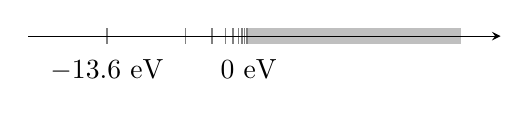
\begin{tikzpicture}[baseline={($ (current bounding box.center)- (0,-6pt) $)}]
\foreach \i in {1,2,...,9,10}{
\draw[gray] (3-2/\i,0.1) -- (3-2/\i,-0.1);
}
\fill[lightgray]  (2.79,0.1) rectangle (5.5,-0.1);
\draw[->] (0,0)--(6,0);
\draw (1,-0.1) node[below=2pt]{$-13.6$ eV};
\draw (2.8,-0.1) node[below=2pt]{$0$ eV};
\end{tikzpicture}
\ei
Note that one of the parts may actually be empty. For instance, as we will later show, the simple quantum harmonic oscillator has the following energy spectrum 
\bi{rCl}
\sigma(H) & =\ & 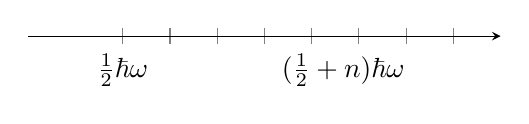
\begin{tikzpicture}[baseline={($ (current bounding box.center)- (0,-7.5pt) $)}]
\foreach \i in {2,...,9}{
\draw[gray] (0.6*\i,0.1) -- (0.6*\i,-0.1);
}
\draw (1.2,-0.1) node[below]{$\tfrac{1}{2}\hbar \omega$};
\draw (4,-0.1) node[below]{$(\tfrac{1}{2}+n)\hbar \omega$};
\draw[->] (0,0)--(6,0);
\end{tikzpicture}
\ei
while the spectrum of the position operator $Q$ is $\sigma(Q) =  \R$.

Also, the continuous part need not be connected, as is the case with spectrum of the Hamiltonian an electron in a periodic potential
\bi{rCl}
\sigma(H) & =\ & 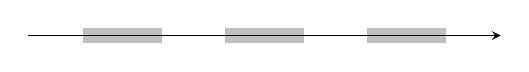
\begin{tikzpicture}
\foreach \i in {0,1,2}{
\fill[lightgray]  (1.8*\i,0.1) rectangle (1+1.8*\i,-0.1);
}
\draw[->] (-0.7,0)--(5.3,0);
\end{tikzpicture}
\ei
It turns out that self-adjoint linear maps on a complex Hilbert space provide a suitable formalism to describe the observables of quantum mechanics. 
\item \textit{An irreducible impact that each measurement has on the state of a quantum system.}

The crucial example demonstrating this is the Stern-Gerlach experiment\index{Stern-Gerlach experiment}, which consists in the following. Silver atoms are heated up in an oven and sent against a screen with a hole. The atoms passing through the hole are then subjected to an inhomogeneous magnetic field, which deflects them according to the component of their angular momentum in the direction of the field. Finally, a screen detects the various deflections.

\begin{center}
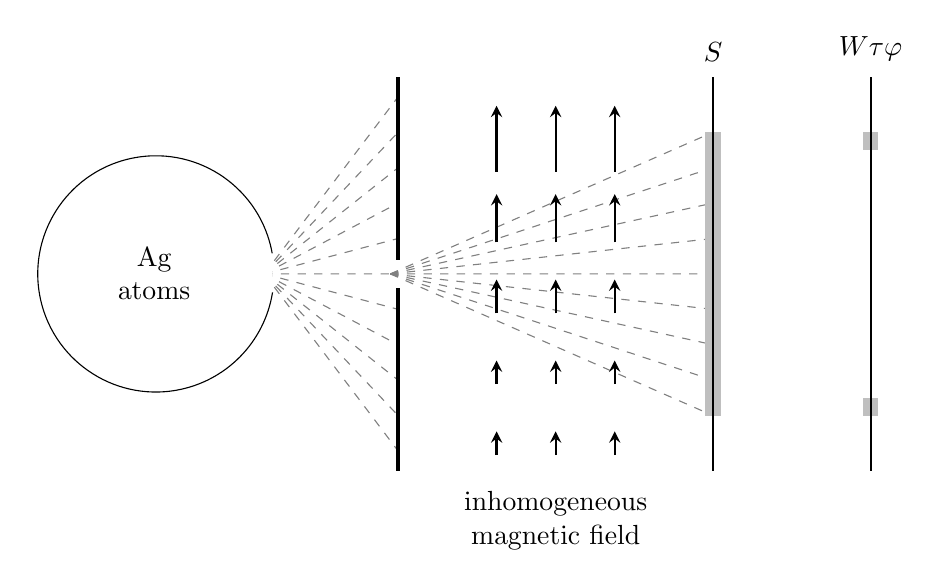
\begin{tikzpicture}[every text node part/.style={align=center}]
\foreach \i in {0,1,...,10} {
\draw[dashed,gray] (0.8,0) -- (2.5,2.25-0.45*\i);
};
\draw[fill=white] (0.9,1.5*sin 10) arc (10:351:1.5);

\draw[ultra thick] (2.5,2.5)--(2.5,0.18);
\draw[ultra thick] (2.5,-0.18)--(2.5,-2.5);
\draw (-0.6,0)  node {Ag\\ atoms};

\foreach \i in {1,...,9} {
\draw[dashed,gray] (2.4,0) -- (6.5,2.25-0.45*\i);
};

\foreach \i in {0,1,...,4} {
  \foreach \j in {1,2,3} {
\draw[thick,->] (3+0.75*\j,-2.3+0.9*\i) -- (3+0.75*\j,-2+0.9*\i^1.1);
};};

\fill[lightgray] (6.5-0.1,2.25-0.45*9) rectangle (6.5+0.1,2.25-0.45);
\draw[thick] (6.5,-2.5)--(6.5,2.5) node[above=2pt] {$S$};

\fill[lightgray] (8.5-0.1,2.25-0.45*9) rectangle (8.5+0.1,2.25-8.5*0.45);
\fill[lightgray] (8.5-0.1,2.25-0.45*1.5) rectangle (8.5+0.1,2.25-0.45);
\draw[thick] (8.5,-2.5)--(8.5,2.5) node[above=2pt] {$W\tau\varphi$};
\draw (4.5,-2.5) node[below=4pt] {inhomogeneous \\ magnetic field};
\end{tikzpicture}
\end{center}

Since the angular momentum distribution of the silver atoms coming from the oven is random, we would expect an even distribution of values of the component along the direction of the magnetic field to be recorded on the final screen, as in $S$. However, the impact pattern actually detected is that on the $W\tau\varphi$ screen. In fact, 50\% of the incoming atoms impact at the top and we say that their angular momentum component is $\uparrow$, and the other 50\% hit the bottom region, and we say that their angular momentum component is $\downarrow$.  This is another instance of our earlier point: there seem to be only two possible values for the component of angular momentum along the direction of the magnetic field, i.e.\ the spectrum is discrete. Hence, this is not particularly surprising at this point.

Let us now consider successive iterations of this experiment. Introduce some system of cartesian coordinates $(x,y,z)$ and let $\mathrm{SG}(x)$ and $\mathrm{SG}(z)$ denotes a Stern-Gerlach apparatus whose magnetic field points in the $x$ and $z$-direction, respectively.

Suppose that we sent the atoms through a first $\mathrm{SG}(z)$ apparatus, and then we use the $z^\uparrow$-output as the input of a second $\mathrm{SG}(z)$ apparatus.
\begin{center}
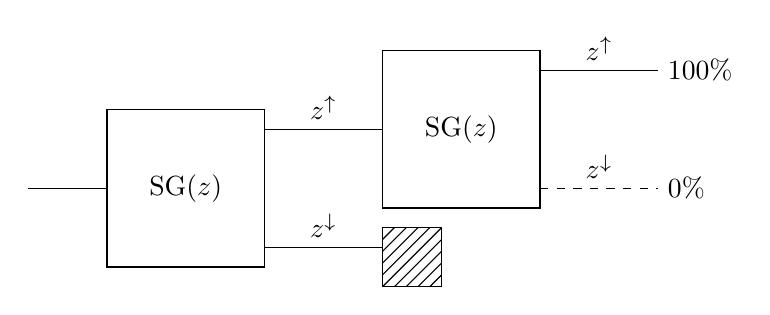
\begin{tikzpicture}[scale=0.5]
\draw (-2,2) -- (0,2);
\draw (2,2) node {$\mathrm{SG}(z)$};
\draw  (0,0) rectangle (4,4);
\draw (4,3.5) -- (7,3.5) node[above,midway] {$z^\uparrow$};
\draw (4,0.5) -- (7,0.5) node[above,midway] {$z^\downarrow$};
\draw  (7,1.5) rectangle (11,5.5);
\draw  (7,1) rectangle (8.5,-0.5);
\draw  (11,5) -- (14,5)  node[above,midway] {$z^\uparrow$} node[right] {100\%};
\draw[dashed]  (11,2) -- (14,2) node[above,midway] {$z^\downarrow$} node[right] {0\%};
\node at (9,3.5) {$\mathrm{SG}(z)$};
\foreach \i in {1,...,5} {
\draw (7+0.3*\i,1)--(7,1-0.3*\i);
\draw (7+0.3*\i,-0.5)--(8.5,1-0.3*\i);
};
\end{tikzpicture}
\end{center}
The second $\mathrm{SG}(z)$ apparatus finds no $z^\downarrow$-atoms. This is not surprising since, intuitively, we ``filtered out'' all the $z^\downarrow$-atoms with the first apparatus. Suppose now that we feed the $z^\uparrow$ output of a $\mathrm{SG}(z)$ apparatus into a $\mathrm{SG}(x)$ apparatus.

\begin{center}
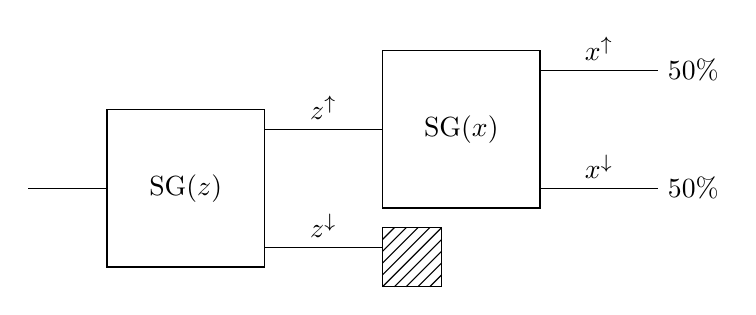
\begin{tikzpicture}[scale=0.5]
\draw (-2,2) -- (0,2);
\draw (2,2) node {$\mathrm{SG}(z)$};
\draw  (0,0) rectangle (4,4);
\draw (4,3.5) -- (7,3.5) node[above,midway] {$z^\uparrow$};
\draw (4,0.5) -- (7,0.5) node[above,midway] {$z^\downarrow$};
\draw  (7,1.5) rectangle (11,5.5);
\draw  (7,1) rectangle (8.5,-0.5);
\draw  (11,5) -- (14,5)  node[above,midway] {$x^\uparrow$} node[right] {50\%};
\draw  (11,2) -- (14,2) node[above,midway] {$x^\downarrow$} node[right] {50\%};
\node at (9,3.5) {$\mathrm{SG}(x)$};
\foreach \i in {1,...,5} {
\draw (7+0.3*\i,1)--(7,1-0.3*\i);
\draw (7+0.3*\i,-0.5)--(8.5,1-0.3*\i);
};
\end{tikzpicture}
\end{center}
Experimentally, we find that about half of the atoms are detected in the state $x^\uparrow$ and half in the state $x^\downarrow$. This is, again, not surprising since we only filtered out the $z^\uparrow$ atoms, and hence we can interpret this result as saying that the $x^\uparrow$, $x^\downarrow$ states are independent from the $z^\uparrow$, $z^\downarrow$.

If our ideas of ``filtering states out'' is correct, then feeding the $x^\uparrow$-output of the previous set-up to another $\mathrm{SG}(z)$ apparatus should clearly produce a $100\%$ $z^\uparrow$-output, since we already filtered out all the $z^\downarrow$ ones in the previous step.

\begin{center}
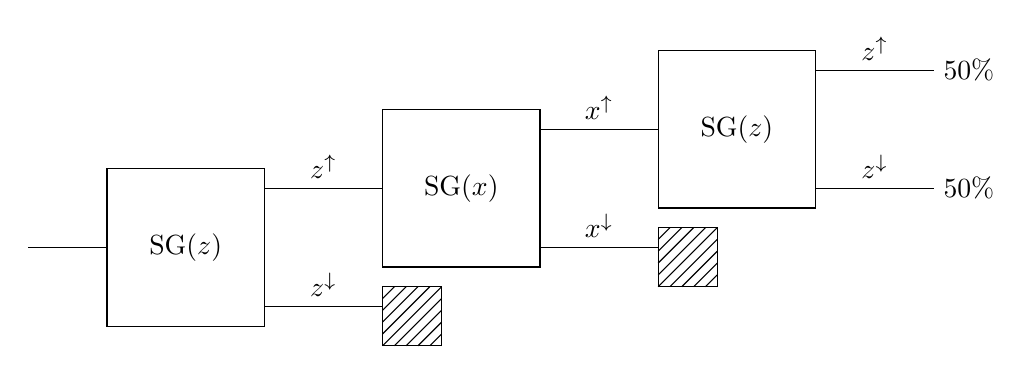
\begin{tikzpicture}[scale=0.5]
\draw (-2,2) -- (0,2);
\draw (2,2) node {$\mathrm{SG}(z)$};
\draw  (0,0) rectangle (4,4);
\draw (4,3.5) -- (7,3.5) node[above,midway] {$z^\uparrow$};
\draw (4,0.5) -- (7,0.5) node[above,midway] {$z^\downarrow$};
\draw  (7,1.5) rectangle (11,5.5);
\draw  (11,5) -- (14,5)  node[above,midway] {$x^\uparrow$} ;
\draw  (11,2) -- (14,2) node[above,midway] {$x^\downarrow$};
\node at (9,3.5) {$\mathrm{SG}(x)$};
\draw  (7,1) rectangle (8.5,-0.5);
\foreach \i in {1,...,5} {
\draw (7+0.3*\i,1)--(7,1-0.3*\i);
\draw (7+0.3*\i,-0.5)--(8.5,1-0.3*\i);
};

\draw  (14,2.5) rectangle (15.5,1);
\foreach \i in {1,...,5} {
\draw (14+0.3*\i,2.5)--(14,2.5-0.3*\i);
\draw (14+0.3*\i,2-1)--(15.5,2.5-0.3*\i);
};
\draw  (14,3) rectangle (18,7);
\draw (16,5) node {$\mathrm{SG}(z)$};
\draw (18,6.5) -- (21,6.5) node[above,midway] {$z^\uparrow$} node[right] {50\%};
\draw (18,3.5) -- (21,3.5) node[above,midway] {$z^\downarrow$} node[right] {50\%};
\end{tikzpicture}
\end{center}
Surprisingly, the output is again $50$-$50$. The idea behind this result is the following. The $\mathrm{SG}(z)$ apparatus left the atoms in a state such that a repeated measurement with the $\mathrm{SG}(z)$ apparatus would give the same result, and similarly for the $\mathrm{SG}(x)$ apparatus. However, the measurement of the $\mathrm{SG}(x)$ apparatus somehow altered the state of the atoms in such a way as to ``reset'' them with respect to a measurement by the $\mathrm{SG}(z)$ apparatus. For more details on the Stern-Gerlach experiment and  further conclusions one can draw from its results, you should consult the book \textit{Modern Quantum Mechanics} by J. J. Sakurai. The conclusion that we are interested in here is that measurements can alter the state of a system.

\item \textit{Even if the state $\rho$ of a quantum system is completely known, the only prediction one can make for the measurement of some observable $A$ is the probability that the measured value, which is an element of the spectrum $\sigma(A)$, lies within a Borel-measurable subset $E\subseteq \R$, denoted by
$\mu^A_{\rho}(E)$}.

In particular, one cannot predict which concrete outcome an isolated measurement will produce. This is even more annoying given that the precise impact that a measurement has on the state of the system (see previous point) depends on the observed outcome of the measurement.
\een

A suitable theory that accommodates all known experimental facts has been developed between 1900 and 1927 on the physics side by, among others, Schr\"odinger, Heisenberg and Dirac, and on the mathematical side almost single-handedly by von Neumann who invented a massive proportion of a field known today as functional analysis.

\subsection{The axioms of quantum mechanics}

We will now present the axioms of quantum mechanics by using notions and terminology that will be defined later in the course. In this sense, this section constitutes a preview of the next few lectures. 

\begin{tcolorbox}[colframe=blue!10!black,before skip=10pt,after skip=10pt]
\begin{axiom}[Quantum systems and states]
To every quantum system there is associated a separable complex Hilbert space $(\mathcal{H},+,\cdot,\langle \cdot | \cdot \rangle)$. The states of the system are all positive, trace-class linear maps $\rho\cl \mathcal{H}\to \mathcal{H}$ for which $\Tr\rho=1$.
\end{axiom}
\end{tcolorbox}

\br
Throughout the quantum mechanics literature, it is stated that the unit, or normalised, elements $\psi\in\mathcal{H}$ (that is, $\langle\psi|\psi\rangle=1$) are the states of the quantum system. This is not correct. 

States can be pure or mixed. A state $\rho\cl \mathcal{H}\to \mathcal{H}$ is called \emph{pure} if
\bse
\exists \, \psi\in \mathcal{H} : \forall \, \alpha\in \mathcal{H} : \ \rho(\alpha) = \frac{\langle\psi|\alpha\rangle}{\langle\psi|\psi\rangle}\psi.
\ese
Thus, we can associate to each pure state $\rho$ an element $\psi\in\mathcal{H}$. However, this correspondence is not one-to-one. Even if we restrict to pure states and impose the normalisation condition, there can be many $\psi\in\mathcal{H}$ representing the same pure state $\rho$. 

Therefore, it is wrong to say that the states of the quantum system are the normalised elements of the Hilbert space, since they do not represent all the states of the system, and do not even represent uniquely the states that they do represent.
\er

The terms used in Axiom 1 are defined as follows.

\bd
A \emph{complex Hilbert space}\index{Hilbert space} is a tuple $(\mathcal{H},+,\cdot,\langle \cdot | \cdot \rangle)$ where
\begin{itemize}
\item $\mathcal{H}$ is a set
\item $+$ is a map $+\cl\mathcal{H}\times \mathcal{H}\to \mathcal{H}$
\item $\cdot$ is a map $\cdot \cl \C \times \mathcal{H}\to \mathcal{H}$ (typically suppressed in the notation)
\end{itemize}
such that the triple $(\mathcal{H},+,\cdot)$ is a vector space over $\C$, and
\begin{itemize}
\item $\langle \cdot | \cdot \rangle$ is a \emph{sesqui-linear\footnote{sesqui is Latin for ``one and a half''.}inner product}, i.e.\ a map $\langle \cdot | \cdot \rangle\cl\mathcal{H}\times \mathcal{H}\to \C$ satisfying
\ben[label=(\roman*)]
\item $\langle \varphi|\psi\rangle=\overline{\langle \psi|\varphi\rangle}$\hfill (conjugate symmetry/Hermitian property)
\item $\langle \varphi|z\psi_1+\psi_2\rangle=z\langle \varphi|\psi_1\rangle+\langle \varphi|\psi_2\rangle$ \hfill (linearity in the second argument)
\item $\langle \psi | \psi\rangle \geq 0$ and $\langle \psi|\psi\rangle = 0 \Leftrightarrow \psi = 0_{\cH}$ \hfill (positive-definiteness)
\een
for all $\varphi,\psi_1,\psi_2\in\mathcal{H}$ and $z\in \C$,
\end{itemize}
and moreover
\begin{itemize}
\item $\mathcal{H}$ is a \emph{complete metric space} with respect to the metric induced by the norm induced in turn by the sesqui-linear map $\langle \cdot | \cdot \rangle$. Explicitly, for every sequence $\phi\cl \N \to \mathcal{H}$ that satisfies the \emph{Cauchy property}, namely
\bse
\forall \, \varepsilon > 0 : \exists \, N\in \N : \forall \, n,m \geq N : \ \|\phi_n-\phi_m\|< \varepsilon,
\ese
where $\phi_n:=\phi(n)$ and $\|\psi\|:=\sqrt{\langle \psi | \psi \rangle}$, then the sequence converges in $\mathcal{H}$, i.e.\
\bse
\exists \, \varphi\in\mathcal{H}:\forall \, \varepsilon > 0 : \exists \, N\in \N : \forall \, n \geq N : \ \|\varphi-\phi_n\|< \varepsilon.
\ese
\end{itemize}
\ed
Note that the $\C$-vector space $(\mathcal{H},+,\cdot)$ need not be finite-dimensional and, in fact, we will mostly work with infinite-dimensional Hilbert spaces. 

\bd
A map $A\cl\mathcal{D}_A\to \mathcal{H}$, where the subspace $\mathcal{D}_A\subseteq \mathcal{H}$ is called the \emph{domain} of $A$, is a \emph{linear map} if
\bse
\forall \, \varphi,\psi\in\mathcal{D}_A:\forall \, z \in \C : \ A(z\varphi+\psi)=zA(\varphi)+A(\psi).
\ese
\ed
From now on, if there is no risk of confusion, we will write $A\varphi:=A(\varphi)$ in order to spare some brackets. We will be particularly interested in special types of linear map.


% \bd
% A linear map $A\cl\mathcal{D}_A\to \mathcal{H}$ is said to be
% \begin{itemize}
% \item \emph{densely defined} if $\mathcal{D}_A$ is \emph{dense} in $\mathcal{H}$, i.e.\
% \bse
% \forall \, \psi\in \mathcal{H} : \exists \, \alpha \in \mathcal{D}_A : \forall \, \varepsilon >0 :\ \|\alpha-\psi\|<\varepsilon
% \ese
% \item \emph{positive} if 
% \bse
% \forall \, \psi\in\mathcal{D}_A : \ \langle\psi|A\psi\rangle\geq 0
% \ese
% \item of \emph{trace-class} if $\mathcal{D}_A=\mathcal{H}$ and, for any orthonormal basis $\{e_n\}$ of $\mathcal{H}$, the sum/series
% \bse
% \sum_n \langle e_n|Ae_n\rangle < \infty.
% \ese
% \end{itemize}
% \ed


\bd
A linear map $A\cl\mathcal{D}_A\to \mathcal{H}$ is \emph{densely defined} if $\mathcal{D}_A$ is \emph{dense} in $\mathcal{H}$, i.e.\
\bse
\forall \, \psi\in \mathcal{H} : \forall \, \varepsilon >0: \exists \, \alpha \in \mathcal{D}_A  :\ \|\alpha-\psi\|<\varepsilon.
\ese
\ed

\bd
A linear map $A\cl\mathcal{D}_A\to \mathcal{H}$ is said to be \emph{positive} if 
\bse
\forall \, \psi\in\mathcal{D}_A : \ \langle\psi|A\psi\rangle\geq 0.
\ese
\ed


\bd
A linear map $A\cl\mathcal{D}_A\to \mathcal{H}$ is said to be of \emph{trace-class} if $\mathcal{D}_A=\mathcal{H}$ and, for any orthonormal basis $\{e_n\}$ of $\mathcal{H}$, the sum/series
\bse
\sum_n \langle e_n|Ae_n\rangle < \infty.
\ese
\ed
If $A\cl\mathcal{H}\to \mathcal{H}$ is of trace-class, one can show that the value of $\sum_n \langle e_n|Ae_n\rangle$ does not depend on the choice of orthonormal basis $\{e_n\}$. 
\bd
Let $A\cl\mathcal{H}\to \mathcal{H}$ be of trace-class. Then the \emph{trace} of $A$ is
\bse
\Tr A :=\sum_n \langle e_n|Ae_n\rangle 
\ese
where $\{e_n\}$ is any orthonormal basis of $\mathcal{H}$.
\ed
\begin{tcolorbox}[colframe=blue!10!black]
\begin{axiom}[Observables]
The observables of a quantum system are the self-adjoint linear maps $A\cl\mathcal{D}_A\to \mathcal{H}$.
\end{axiom}
\end{tcolorbox}
While the notion of a self-adjoint map is easy to define in finite-dimensional spaces, it is much more subtle for infinite-dimensional spaces.

\bd
A densely defined linear map $A\cl\mathcal{D}_A\to \mathcal{H}$ is said to be of \emph{self-adjoint} if it coincides with its adjoint map $A^*\cl\mathcal{D}_{A^*}\to \mathcal{H}$, that is
\begin{itemize}
\item $\mathcal{D}_A=\mathcal{D}_{A^*}$
\item $\forall \, \varphi\in\mathcal{D}_A : \ A\varphi=A^*\varphi$.
\end{itemize}
\ed
%The subtle part is the definition of the adjoint map itself.
\bd
The \emph{adjoint map} $A^*\cl\mathcal{D}_{A^*}\to \mathcal{H}$ of a linear map $A\cl\mathcal{D}_A\to \mathcal{H}$ is defined by
\begin{itemize}
\item $\mathcal{D}_{A^*}:=\{\psi\in\mathcal{H}\mid \forall \, \alpha \in \mathcal{D}_A:\exists \, \eta \in \mathcal{H} : \langle\psi|A\alpha\rangle=\langle\eta|\alpha\rangle\}$
\item $A^*\psi:=\eta$.
\end{itemize}
\ed
We will later show that the adjoint map is well-defined, i.e.\ for each $\alpha\in\mathcal{D}_A$ and $\psi\in\mathcal{H}$ there exists at most one $\eta\in\mathcal{H}$ such that $\langle\psi|A\alpha\rangle = \langle\eta|\alpha\rangle$.

\br
If we defined $\mathcal{D}_{A^*}$ by requiring that $\eta\in \mathcal{D}_{A}$, we would obtain a notion of self-adjointness which has undesirable properties. In particular, the spectrum (to be defined later) of a self-adjoint operator would not be guaranteed to be a subset of $\R$.
\er

\begin{tcolorbox}[colframe=blue!10!black]
\begin{axiom}[Measurement]
The probability that a measurement of an observable $A$ on a system that is in the state $\rho$ yields a result in the Borel set $E\subseteq \R$ is given by
\bse
\mu^A_\rho(E):=\Tr(\mathrm{P}_{\!A}(E)\circ\rho)
\ese
where the map $\mathrm{P}_{\!A}\cl \Borel(\R)\to\mathcal{L}(\mathcal{H})$, from the Borel-measurable subsets of $\R$ to the Banach space of bounded linear maps on $\mathcal{H}$, is the unique projection-valued measure that is associated with the self-adjoint map $A$ according to the spectral theorem.\end{axiom}\end{tcolorbox}

We will later see that the composition of a bounded linear map with a trace-class map is again of trace-class, so that $\Tr(\mathrm{P}_{\!A}(E)\circ\rho)$ is well-defined. For completeness, the spectral theorem states that for any self-adjoint map $A$ there exists a projection-valued measure $\mathrm{P}_{\!A}$ such that $A$ can be represented in terms of the Lebesgue-Stieltjes integral as
\bse
A = \int_{\R}\lambda \, \d \mathrm{P}_{\!A}(\lambda).
\ese
This is the infinite-dimensional analogue of the diagonalisation theorem for symmetric or Hermitian matrices on finite-dimensional vector spaces, and it is the theorem in which the first half of the course will find its climax.


\begin{tcolorbox}[colframe=blue!10!black,before skip=10pt]
\begin{axiom}[Unitary dynamics]
In a time interval $(t_1,t_2)\subseteq \R$ in which no measurement occurs, the state $\rho$ at time $t_1$, denoted $\rho(t_1)$, is related to the state $\rho$ at time $t_2$, denoted $\rho(t_2)$, by
\bse
\rho(t_2) = U(t_2-t_1)\rho(t_1) U^{-1}(t_2-t_1)
\ese
with the unitary evolution operator $U$ defined as
\bse
U(t) := \exp(-\tfrac{\mathrm{i}}{\hbar}Ht),
\ese
where $H$ is the energy observable and, for any observable $A$ and $f\cl \R\to \C$, we define
\bse
f(A):=\int_\R f(\lambda) \, \d \mathrm{P}_{\!A}(\lambda).
\ese
\end{axiom}
\end{tcolorbox}
Note that, as was the case for the previous axiom, the spectral theorem is crucial since it is needed to define  the unitary evolution operator.

\begin{tcolorbox}[colframe=blue!10!black,before skip=10pt]
\begin{axiom}[Projective dynamics]
The state $\rho_{\mathrm{after}}$ of a quantum system immediately following the measurement of an observable $A$ is
\bse
\rho_{\mathrm{after}} := \frac{\mathrm{P}_{\!A}(E)\circ\rho_{\mathrm{before}}\circ\mathrm{P}_{\!A}(E)}{\Tr(\mathrm{P}_{\!A}(E)\circ\rho_{\mathrm{before}}\circ\mathrm{P}_{\!A}(E))}
\ese
where $\rho_{\mathrm{before}}$ is the state immediately preceding the measurement and $E\subseteq\R$ is the smallest Borel set in which the actual outcome of the measurement happened to lie.
\end{axiom}
\end{tcolorbox}
























\newpage

\section{Banach spaces}

Hilbert spaces are a special type of a more general class of spaces known as Banach spaces. We are interested in Banach spaces not just for the sake generality, but also because they naturally appear in Hilbert space theory. For instance, the space of bounded linear maps on a Hilbert space is not itself a Hilbert space, but only a Banach space.

\subsection{Generalities on Banach spaces}

We begin with some basis notions from metric space theory.

\bd
A \emph{metric space}\index{metric space} is a pair $(X,d)$, where $X$ is a set and $d$ is a \emph{metric} on $X$, that is, a map $d\cl X\times X \to \R$ satisfying
\ben[label=(\roman*)]
\item $d(x,x)\geq 0$ \hfill (non-negativity)
\item $d(x,y) = 0\ \Leftrightarrow \ x=y$ \hfill (identity of indiscernibles)
\item $d(x,y)=d(y,x)$ \hfill (symmetry)
\item $d(x,z)\leq d(x,y)+d(y,z)$ \hfill (triangle inequality)
\een
for all $x,y,z\in X$.
\ed

\bd
A sequence $\{x_n\}_{n\in \N}$ in a metric space $(X,d)$ is said to \emph{converge}\index{convergence} to an element $x\in X$, written $\displaystyle \lim_{n\to \infty}x_n=x$, if
\bse
\forall \, \varepsilon > 0 : \exists \, N \in \N : \forall \, n \geq N : \ d(x_n,x)<\varepsilon.
\ese
\ed

A sequence in a metric space can converge to at most one element.

\bd
A \emph{Cauchy sequence}\index{Cauchy sequence} in a metric space $(X,d)$ is a sequence $\{x_n\}_{n\in \N}$ such that
\bse
\forall \, \varepsilon > 0 : \exists \, N \in \N : \forall \, n,m \geq N : \ d(x_n,x_m)<\varepsilon.
\ese
\ed
Any convergent sequence is clearly a Cauchy sequence.

\vbox{\bd
A metric space $(X,d)$ is said to be \emph{complete}\index{completeness} if every Cauchy sequence converges to some $x\in X$.
\ed
A natural metric on a vector space is that induced by a norm.

\noindent Note that every convergent sequence is a Cauchy sequence, the converse does not hold in general.

\bd
A \emph{normed space}\index{normed space} is a (complex) vector space $(V,+,\cdot)$ equipped with a \emph{norm}, that is, a map $\|\cdot\|\cl V \to \R$ satisfying
\ben[label=(\roman*)]
\item $\|f\|\geq 0$ \hfill (non-negativity)
\item $\|f\| = 0 \ \Leftrightarrow\ f=0$ \hfill (definiteness)
\item $\|z\cdot f\|=|z|\|f\|$ \hfill (homogeneity/scalability)
\item $\|f+g\|\leq \|f\|+\|g\|$ \hfill (triangle inequality/sub-additivity)
\een
for all $f,g\in V$ and all $z\in \C$.
\ed}
Once we have a norm $\|\cdot\|$ on $V$, we can define a metric $d$ on $V$ by 
\bse
d(f,g) := \|f-g\|.
\ese
Then we say that the normed space $(V,\|\cdot\|)$ is \emph{complete} if the metric space $(V,d)$, where $d$ is the metric induced by $\|\cdot\|$, is complete. Note that we will usually suppress inessential information in the notation, for example writing $(V,\|\cdot\|)$ instead of $(V,+,\cdot,\|\cdot\|)$.

\bd
A \emph{Banach space}\index{Banach space} is a complete normed vector space.
\ed

% This example and proof are commented out because Simon is now convinced it's wrong and needs editing. 
%\be
%The space $C^0_\C[0,1]:=\{f\cl [0,1]\to \C \mid f \text{ is continuous}\}$, where the continuity is with respect to the standard topologies on $[0,1]\subset \R$ and $\C$, is a Banach space. Let us show this in some detail.
%\bq
%\ben[label=(\alph*)]
%\item First, define two operations $+,\cdot$ pointwise, that is, for any $x\in [0,1]$
%\bse
%(f+g)(x) := f(x)+g(x)\qquad \quad (z\cdot f)(x):=zf(x).
%\ese
%Suppose that $f,g\in C^0_\C[0,1]$, that is
%\bse
%\forall \, x_0\in [0,1]: \forall \, \varepsilon > 0 : \exists \, \delta > 0 : \forall \, x\in (x_0-\delta,x_0+\delta) : \ |f(x)-f(x_0)|<\varepsilon
%\ese
%and similarly for $g$. Fix $x_0\in[0,1]$ and $\varepsilon >0$. Then, there exist $\delta_1,\delta_2>0$ such that
%\bi{c}
%\forall \, x\in (x_0-\delta_1,x_0+\delta_1) : \ |f(x)-f(x_0)|<\tfrac{\varepsilon}{2}\phantom{.}\\
%\forall \, x\in (x_0-\delta_2,x_0+\delta_2) : \ |g(x)-g(x_0)|<\tfrac{\varepsilon}{2}.
%\ei
%Let $\delta:=\min\{\delta_1,\delta_2\}$. Then, for all $x\in (x_0-\delta,x_0+\delta)$, we have
%\bi{rCl}
%|(f+g)(x)-(f+g)(x_0)| & := & |f(x)+g(x)-(f(x_0)+g(x_0))|\\
% & = & |f(x)-f(x_0)+g(x)-g(x_0))|\\
% & \leq & |f(x)-f(x_0)|+|g(x)-g(x_0))|\\
%& < & \tfrac{\varepsilon}{2}+\tfrac{\varepsilon}{2}\\
%& = & \varepsilon.
%\ei
%Since $x_0\in[0,1]$ was arbitrary, we have $f+g\in C^0_\C[0,1]$. Similarly, for any $z\in \C$ and $f\in C^0_\C[0,1]$, we also have $z\cdot f\in C^0_\C[0,1]$. It is immediate to check that the complex vector space structure of $\C$ implies that the operations
%\bi{rrClcrrCl}
%+\cl & C^0_\C[0,1] \times C^0_\C[0,1] & \to & C^0_\C[0,1] &\quad \qquad & \cdot \cl &\C \times C^0_\C[0,1] & \to & C^0_\C[0,1]\\
%& (f,g) &\mapsto & f+g && & (z,f) & \mapsto & z\cdot f
%\ei
%make $(C^0_\C[0,1],+,\cdot)$ into a complex vector space.

%\item Since $[0,1]$ is closed and bounded, it is compact and hence every complex-valued continuous function $f\cl [0,1]\to \C$ is bounded, in the sense that
%\bse
%\sup_{x\in[0,1]}|f(x)| < \infty.
%\ese
%We can thus define a norm on $C^0_\C[0,1]$, called the \emph{supremum} (or \emph{infinity}) \emph{norm}, by
%\bse
%\|f\|_{\infty} := \sup_{x\in[0,1]}|f(x)| .
%\ese
%Let us show that this is indeed a norm on $(C^0_\C[0,1],+,\cdot)$ by checking that the four defining properties hold. Let $f,g\in C^0_\C[0,1]$ and $z\in \C$. Then
%\ben[label=(b.\roman*)]
%\item $\displaystyle \|f\|_{\infty}:= \sup_{x\in[0,1]}|f(x)| \geq 0$ since $|f(x)|\geq 0$ for all $x\in [0,1]$.
%\item $\displaystyle \|f\|_{\infty}=0\ \Leftrightarrow \sup_{x\in[0,1]}|f(x)| = 0$. By definition of supremum, we have
%\bse
%\forall \, x \in [0,1] : \ |f(x)|\leq \sup_{x\in[0,1]}|f(x)| = 0. 
%\ese
%But since we also have $|f(x)|\geq 0$ for all $x\in [0,1]$, $f$ is identically zero.
%\item $\displaystyle \|z\cdot f\|_{\infty} := \sup_{x\in[0,1]}|zf(x)| = \sup_{x\in[0,1]}|z||f(x)|=|z|\sup_{x\in[0,1]}|f(x)| = |z|\|f\|_{\infty}$.
%\item By using the triangle inequality for the modulus of complex numbers, we have
%\bi{rCl}
%\|f+g\|_{\infty} &:=& \sup_{x\in[0,1]}|(f+g)(x)|\\
%&=& \sup_{x\in[0,1]}|f(x)+g(x)|\\
%&\leq & \sup_{x\in[0,1]}(|f(x)|+|g(x)|)\\
%& = & \sup_{x\in[0,1]}|f(x)|\,+\sup_{x\in[0,1]}|g(x)|\\
%& = & \|f\|_{\infty}+\|g\|_{\infty}.
%\ei
%Hence, $(C^0_\C[0,1],\|\cdot\|_{\infty})$ is indeed a normed space.
%\een
%\item We now show that $C^0_\C[0,1]$ is complete. Let $\{f_n\}_{n\in \N}$ be a Cauchy sequence of functions in $C^0_\C[0,1]$, that is
%\bse
%\forall \, \varepsilon > 0 : \exists \, N \in \N : \forall \, n,m \geq N : \ \|f_n-f_m\|_{\infty} <\varepsilon.
%\ese
%We seek an $f\in C^0_\C[0,1]$ such that $\displaystyle \lim_{n\to\infty}f_n=f$. We will proceed in three steps.
%\ben[label=(c.\roman*)]
%\item Fix $y\in [0,1]$ and $\varepsilon >0$. By definition of supremum, we have
%\bse
%|f_n(y) -f_m(y)| \leq \sup_{x\in[0,1]}|f_n(x)-f_m(x)| =: \|f_n-f_m\|_{\infty}.
%\ese
%Hence, there exists $N\in \N$ such that
%\bse
%\forall \, n,m \geq N : \ |f_n(y) -f_m(y)|<\varepsilon,
%\ese
%that is, the sequence of complex numbers $\{f_n(y)\}_{n\in \N}$ is a Cauchy sequence. Since $\C$ is a complete metric space\footnote{The standard metric on $\C$ is induced by the modulus of complex numbers.}, there exists $z_y\in\C$ such that $\displaystyle \lim_{n\to \infty}f_n(y)=z_y$. 

%Thus, we can define a function
%\bi{rrCl}
%f\cl & [0,1] & \to & \C\\
%& x & \mapsto & z_x,
%\ei
%called the \emph{pointwise limit} of $f$, which by definition satisfies
%\bse
%\forall \, x \in [0,1] : \ \lim_{n\to \infty}f_n(x)=f(x).
%\ese
%Note that this does \emph{not} automatically imply that $\displaystyle \lim_{n\to \infty}f_n=f$ (converge with respect to the supremum norm), nor that $f\in C^0_\C[0,1]$, and hence we need to check separately that these do, in fact, hold.
%\item First, let us check that $f\in C^0_\C[0,1]$, that is, $f$ is continuous. Let $x_0\in [0,1]$ and $\varepsilon>0$. For each $x\in [0,1]$, we have
%\bi{rCl}
%|f(x)-f(x_0)| & = & |f(x)-f_n(x)+f_n(x)-f_n(x_0)+f_n(x_0)-f(x_0)|\\
% & \leq & |f(x)-f_n(x)|+|f_n(x)-f_n(x_0)|+|f_n(x_0)-f(x_0)|.
%\ei
%Since $f$ is the pointwise limit of $\{f_n\}_{n\in\N}$, for each $x\in[0,1]$ there exists $N\in \N$ such that
%\bse
%\forall \, n \geq N : \ |f(x)-f_n(x)|<\tfrac{\varepsilon}{3}.
%\ese
%In particular, we also have
%\bse
%\forall \, n \geq N : \ |f_n(x_0)-f(x_0)|<\tfrac{\varepsilon}{3}.
%\ese
%Moreover, since $f_n\in C^0_\C[0,1]$ by assumption, there exists $\delta>0$ such that
%\bse
%\forall \, x\in (x_0-\delta,x_0+\delta)  : \ |f_n(x)-f_n(x_0)|<\tfrac{\varepsilon}{3}.
%\ese
%Fix $n\geq N$. Then, it follows that for all $x\in (x_0-\delta,x_0+\delta)$, we have
%\bi{rCl}
%|f(x)-f(x_0)|  & \leq & |f(x)-f_n(x)|+|f_n(x)-f_n(x_0)|+|f_n(x_0)-f(x_0)|\\
%& < & \tfrac{\varepsilon}{3}+\tfrac{\varepsilon}{3}+\tfrac{\varepsilon}{3}\\
%& = & \varepsilon.
%\ei
%Since $x_0\in[0,1]$ was arbitrary, we have $f\in C^0_\C[0,1]$.
%\item Finally, it remains to show that $\displaystyle \lim_{n\to \infty}f_n=f$. To that end, let $\varepsilon>0$. By the triangle inequality for $\|\cdot\|_{\infty}$, we have
%\bi{rCl}
%\|f_n-f\|_{\infty} &=& \|f_n-f_m+f_m-f\|_{\infty}\\
%&\leq& \|f_n-f_m\|_{\infty}+\|f_m-f\|_{\infty}.
%\ei
%Since $\{f_n\}_{n\in\N}$ is Cauchy by assumption, there exists $N_1\in \N$ such that
%\bse
%\forall \, n,m\geq N_1 : \ \|f_n-f_m\|_{\infty} < \tfrac{\varepsilon}{2}.
%\ese
%Moreover, since $f$ is the pointwise limit of $\{f_n\}_{n\in\N}$, for each $x\in[0,1]$ there exists $N_2\in \N$ such that
%\bse
%\forall \, m \geq N_2 : \ |f_m(x)-f(x)|<\tfrac{\varepsilon}{2}.
%\ese
%By definition of supremum, we have
%\bse
%\forall \, m \geq N_2 : \ \|f_m-f\|_{\infty}= \sup_{x\in[0,1]}|f_m(x)-f(x)|\leq\tfrac{\varepsilon}{2}.
%\ese
%Let $N:=\max\{N_1,N_2\}$ and fix $m\geq N$. Then, for all $n\geq N$, we have
%\bi{c}
%\|f_n-f\|_{\infty} \leq \|f_n-f_m\|_{\infty}+\|f_m-f\|_{\infty} < \tfrac{\varepsilon}{2} + \tfrac{\varepsilon}{2} = \varepsilon.
%\ei
%Thus, $\displaystyle \lim_{n\to \infty}f_n = f$ and we call $f$ the \emph{uniform limit} of $\{f_n\}_{n\in\N}$.
%\een
%\een
%This completes the proof that $(C^0_\C[0,1],\|\cdot\|_{\infty})$ is a Banach space.
%\eq
%\ee

%\br
%The previous example shows that checking that something is a Banach space, and the completeness property in particular, can be quite tedious. However, in the following, we will typically already be working with a Banach (or Hilbert) space and hence, rather than having to check that the completeness property holds, we will instead be able to use it to infer the existence (within that space) of the limit of any Cauchy sequence.
%\er

\subsection{Bounded linear operators}

As usual in mathematics, once we introduce a new types of structure, we also want study maps between instances of those structures, with extra emphasis placed on the structure-preserving maps. We begin with linear maps from a normed space to a Banach space.

\bd
Let $(V,\|\cdot\|_V)$ be a normed space and $(W,\|\cdot\|_W)$ a Banach space. A linear map, also called a linear operator, $A\cl V\to W$ is said to be \emph{bounded} if
\bse
\sup_{f\in V}\frac{\|Af\|_W}{\|f\|_V} < \infty.
\ese
\ed
Note that the quotient is not defined for $f=0$. Hence, to be precise, we should write $V\setminus\{0\}$ instead of just $V$. Let us agree that is what mean in the above definition. There are several equivalent characterisations of the boundedness property.

\vbox{
\bp
\label{prp:boundequiv}
A linear operator $A\cl V\to W$ is bounded if, and only if, any of the following conditions are satisfied.
\ben[label=(\roman*)]
\item $\displaystyle \sup_{\|f\|_V=1}\|Af\|_W< \infty$
\item $\exists \, k > 0 : \forall \, f\in V: \ \|f\|_V \leq 1\, \Rightarrow \, \|Af\|_W \leq k$
\item $\exists \, k > 0 : \forall \, f\in V: \ \|Af\|_W\leq  k \|f\|_V$
\item the map $A\cl V \to W$ is continuous with respect to the topologies induced by the respective norms on $V$ and $W$
\item the map $A$ is continuous at $0\in V$. 
\een
\ep}

The first one of these follows immediately from the homogeneity of the norm. Indeed, suppose that $\|f\|_V\neq 1$. Then
\bse
\frac{\|Af\|_W}{\|f\|_V} = \|f\|_V^{-1}\|Af\|_W =\|A(\|f\|_V^{-1} f)\|_W = \|A\widetilde f\|_W 
\ese
where $\widetilde f:= \|f\|_V^{-1}f$ is such that $\|\widetilde f\|_V=1$. Hence, the boundedness property is equivalent to condition (i) above. 

\bd
Let $A\cl V \to W$ be a bounded operator. The \emph{operator norm}\index{operator norm} of $A$ is defined as
\bse
\|A\|:=\sup_{\|f\|_V=1} \|Af\|_W = \sup_{f\in V}\frac{\|Af\|_W}{\|f\|_V} .
\ese
\ed

\be
Let $\id_W\cl W\to W$ be the identity operator on a Banach space $W$. Then
\bse
\sup_{f\in W}\frac{\|\id_Wf\|_W}{\|f\|_W} =\sup_{f\in W}1 = 1 <\infty.
\ese
Hence, $\id_W$ is a bounded operator and has unit norm.
\ee

\be
Denote by $C^1_{\C}[0,1]$ the complex vector space of once continuously differentiable complex-valued functions on $[0,1]$. Since differentiability implies continuity, this is a subset of $C^0_{\C}[0,1]$. Moreover, since sums and scaling by a complex number of continuously differentiable functions are again continuously differentiable, this is, in fact, a vector subspace of $C^0_{\C}[0,1]$, and hence also a normed space with the supremum norm $\|\cdot\|_{\infty}$.

Consider the first derivative operator
\bi{rrCl}
D \cl & C^1_{\C}[0,1] & \to & C^0_{\C}[0,1]\\
& f & \mapsto & f'.
\ei
We know from undergraduate real analysis that $D$ is a linear operator. We will now show that $D$ is an unbounded\footnote{Some people take the term unbounded to mean ``not necessarily bounded''. We take it to mean ``definitely not bounded'' instead.} linear operator. That is,
\bse
\sup_{f\in C^1_{\C}[0,1]} \frac{\|Df\|_{\infty}}{\|f\|_{\infty}} = \infty.
\ese
Note that, since the norm is a function into the real numbers, both $\|Df\|_{\infty}$ and $\|f\|_{\infty}$ are always finite for any $f\in C^1_{\C}[0,1]$. Recall that the supremum of a set of real numbers is its least upper bound and, in particular, it need not be an element of the set itself. What we have to show is that the set
\bse
\biggl\{ \frac{\|Df\|_{\infty}}{\|f\|_{\infty}} \ \Big| \ f\in C^1_{\C}[0,1] \biggr\} \subset \R
\ese
contains arbitrarily large elements. One way to do this is to exhibit a positively divergent (or unbounded from above) sequence within the set. 

Consider the sequence $\{f_n\}_{n\geq 1}$ where $f_n(x):=\sin(2\pi nx)$. We know that sine is continuously differentiable, hence $f_n\in C^1_{\C}[0,1]$ for each $n\geq 1$, with
\bse
Df_n(x) = D(\sin(2\pi nx)) = 2\pi n\cos(2\pi nx).
\ese
We have
\bse
\|f_n\|_{\infty} = \sup_{x\in[0,1]}|f_n(x)| = \sup_{x\in[0,1]}|\sin(2\pi nx)| = \sup \, [-1,1] = 1 
\ese
and
\bse
\|Df_n\|_{\infty} = \sup_{x\in[0,1]}|Df_n(x)| = \sup_{x\in[0,1]}|2\pi n\cos(2\pi nx)| = \sup\, [-2\pi n,2\pi n] = 2\pi n.
\ese
Hence, we have
\bse
\sup_{f\in C^1_{\C}[0,1]} \frac{\|Df\|_{\infty}}{\|f\|_{\infty}} \geq \sup_{\{f_n\}_{n\geq 1}} \frac{\|Df\|_{\infty}}{\|f\|_{\infty}} = \sup_{n\geq 1}\,2\pi n = \infty,
\ese
which is what we wanted. As an aside, we note that $C^1_{\C}[0,1]$ is not complete with respect to the supremum norm, but it is complete with respect to the norm
\bse
\|f\|_{C^1}:=\|f\|_{\infty}+\|f'\|_{\infty}.
\ese
While the derivative operator is still unbounded with respect to this new norm, in general, the boundedness of a linear operator does depend on the choice of norms on its domain and target, as does the numerical value of the operator norm.
\ee

\br
Apart from the ``minor'' detail that in quantum mechanics we deal with Hilbert spaces, use a different norm than the supremum norm and that the (one-dimensional) momentum operator acts as $P(\psi):=-\mathrm{i}\hbar\psi'$, the previous example is a harbinger of the fact that the momentum operator in quantum mechanics is unbounded. This will be the case for the position operator $Q$ as well.
\er
\bl
\label{lem:forcompl}
Let $(V,\|\cdot\|)$ be a normed space. Then, addition, scalar multiplication, and the norm are all sequentially continuous. That is, for any sequences $\{f_n\}_{n\in \N}$ and $\{g_n\}_{n\in \N}$ in $V$ converging to $f\in V$ and $g\in V$ respectively, and any sequence $\{z_n\}_{n\in \N}$ in $\C$ converging to $z\in \C$, we have
\ben[label=(\roman*)]
\item $\displaystyle \lim_{n\to \infty}(f_n+g_n)=f+g$
\item $\displaystyle \lim_{n\to \infty}z_nf_n=zf$.
\item $\displaystyle \lim_{n\to \infty}\|f_n\|=\|f\|$
\een
\el

\bq
\ben[label=(\roman*)]
\item Let $\varepsilon >0$. Since $\displaystyle \lim_{n\to \infty}f_n=f$ and $\displaystyle \lim_{n\to \infty}g_n=g$ by assumption, there exist $N_1,N_2\in \N$ such that
\bi{c}
\forall \, n\geq N_1 : \ \|f-f_n\|<\tfrac{\varepsilon}{2}\phantom{.}\\
\forall \, n\geq N_2 : \ \|g-g_n\|<\tfrac{\varepsilon}{2}.
\ei
Let $N:=\max\{N_1,N_2\}$. Then, for all $n\geq N$, we have
\bi{rCl}
\|(f_n+g_n)-(f+g)\| &=& \|f_n-f+g_n-g\|\\
&\leq& \|f_n-f\|+\|g_n-g\|\\
& < & \tfrac{\varepsilon}{2}+\tfrac{\varepsilon}{2}\\
& = & \varepsilon.
\ei
Hence $\displaystyle \lim_{n\to \infty}(f_n+g_n)=f+g$.


\item Since $\{z_n\}_{n\in \N}$ is a convergent sequence in $\C$, it is bounded. That is,
\bse
\exists \, k>0 : \forall \, n\in \N : \ |z_n|\leq k.
\ese
Let $\varepsilon >0$. Since $\displaystyle \lim_{n\to \infty}f_n=f$ and $\displaystyle \lim_{n\to \infty}z_n=z$, there exist $N_1,N_2\in \N$ such that
\bi{l}
\forall \, n\geq N_1 : \ \|f-f_n\|<\frac{\varepsilon}{2k}\\
\forall \, n\geq N_2 : \ \|z-z_n\|<\frac{\varepsilon}{2\|f\|}.
\ei
Let $N:=\max\{N_1,N_2\}$. Then, for all $n\geq N$, we have
\bi{rCl}
\|z_nf_n-zf\| &=& \|z_nf_n-z_nf+z_nf-zf\|\\
&=& \|z_n(f_n-f)+(z_n-z)f\|\\
&\leq& \|z_n(f_n-f)\|+\|(z_n-z)f\|\\
&=& |z_n|\|f_n-f\|+|z_n-z|\|f\|\\
& < & k\frac{\varepsilon}{2k}+\frac{\varepsilon}{2\|f\|}\|f\|\\
& = & \varepsilon.
\ei
Hence $\displaystyle \lim_{n\to \infty}z_nf_n=zf$.
\item Let $\varepsilon >0$. Since  $\displaystyle \lim_{n\to \infty}f_n=f$, there exists $N\in \N$ such that
\bse
\forall \, n \geq N : \ \|f_n-f\|<\varepsilon.
\ese
By the triangle inequality, we have
\bse
\|f_n\| = \|f_n-f+f\| \leq \|f_n-f\|+\|f\|  
\ese
so that $\|f_n\|-\|f\|\leq \|f_n-f\|$. Similarly, $\|f\|-\|f_n\|\leq \|f-f_n\|$. Since
\bse
\|f-f_n\| = \|-(f_n-f)\| = |-1|\|f_n-f\| = \|f_n-f\|,
\ese
we have $-\|f_n-f\|\leq\|f_n\|-\|f\|\leq\|f_n-f\|$ or, by using the modulus,
\bse
\bigl| \|f_n\|-\|f\|\bigr| \leq \|f_n-f\|.
\ese
Hence, for all $n\geq N$, we have $\bigl| \|f_n\|-\|f\|\bigr| <\varepsilon$ and thus  $\displaystyle \lim_{n\to \infty}\|f_n\|=\|f\|$.
\qedhere
\een
\eq
Note that by taking $\{z_n\}_{n\in\N}$ to be the constant sequence whose terms are all equal to some fixed $z\in \C$, we have $\displaystyle \lim_{n\to \infty}zf_n=zf$ as a special case of (ii).

This lemma will take care of some of the technicalities involved in proving the following crucially important result.

\begin{theorem}
\label{thrm:BoundedLinearOperatorsBanach}
The set $\mathcal{L}(V,W)$ of bounded linear operators from a normed space $(V,\|\cdot\|_V)$ to a Banach space $(W,\|\cdot\|_W)$, equipped with pointwise addition and scalar multiplication and the operator norm, is a Banach space.
\end{theorem}

\bq
\ben[label=(\alph*)]
\item Define addition and scalar multiplication on $\mathcal{L}(V,W)$ by
\bse
(A+B)f := Af+Bf \quad \qquad (zA)f := zAf.
\ese
It is clear that both $A+B$ and $zA$ are linear operators.  Moreover, we have
\bi{rCl}
\sup_{f\in V}\frac{\|(A+B)f\|_W}{\|f\|_V} &:=& \sup_{f\in V}\frac{\|Af+Bf\|_W}{\|f\|_V} \\
 &\leq & \sup_{f\in V}\frac{\|Af\|_W+\|Bf\|_W}{\|f\|_V} \\
 &=& \sup_{f\in V}\frac{\|Af\|_W}{\|f\|_V} + \sup_{f\in V}\frac{\|Bf\|_W}{\|f\|_V} \\
 &<& \infty
\ei
since $A$ and $B$ are bounded. Hence, $A+B$ is also bounded and we have
\bse
\|A+B\|\leq \|A\|+\|B\|.
\ese
Similarly, for $zA$ we have 
\bi{rCl}
\sup_{f\in V}\frac{\|(zA)f\|_W}{\|f\|_V} &:=& \sup_{f\in V}\frac{\|zAf\|_W}{\|f\|_V} \\
 &= & \sup_{f\in V}\frac{|z|\|Af\|_W}{\|f\|_V} \\
 &=& |z|\sup_{f\in V}\frac{\|Af\|_W}{\|f\|_V} \\
 &<& \infty
\ei
since $A$ is bounded and $|z|$ is finite. Hence, $zA$ is bounded and we have
\bse
\|zA\|=|z|\|A\|.
\ese
Thus, we have two operations
\bi{rrClcrrCl}
+\cl & \mathcal{L}(V,W)\times \mathcal{L}(V,W) & \to & \mathcal{L}(V,W) &\qquad \quad & \cdot \cl & \C \times \mathcal{L}(V,W) & \to & \mathcal{L}(V,W)\\
& (A,B) & \mapsto & A+B && & (z,A) & \mapsto & zA
\ei
and it is immediate to check that the vector space structure of $W$ induces a vector space structure on $\mathcal{L}(V,W)$ with these operations.

\item We need to show that $(\mathcal{L}(V,W),\|\cdot\|)$ is a normed space, i.e.\ that $\|\cdot\|$ satisfies the properties of a norm. We have already shown two of these in part (a), namely
\ben[label=(b.\roman*),start=3]
\item $\|zA\|=|z|\|A\|$
\item $\|A+B\|\leq \|A\|+\|B\|$.
\een
The remaining two are easily checked.
\ben[label=(b.\roman*)]
\item $\displaystyle \|A\|:=\sup_{f\in V}\frac{\|Af\|_W}{\|f\|_V}\geq 0$ since $\|\cdot\|_V$ and $\|\cdot\|_W$ are norms.
\item Again, by using the fat that $\|\cdot\|_W$ is a norm,
\bi{rCl"s}
\|A\|=0 &\ \Leftrightarrow\ & \sup_{f\in V}\frac{\|Af\|_W}{\|f\|_V}= 0\\
& \Leftrightarrow & \forall \, f\in V:\ \|Af\|_W=0\\
& \Leftrightarrow & \forall \, f\in V:\ Af=0\\
& \Leftrightarrow & \ A=0.
\ei
\een
Hence, $(\mathcal{L}(V,W),\|\cdot\|)$ is a normed space.

\item The heart of the proof is showing that $(\mathcal{L}(V,W),\|\cdot\|)$ is complete. We will proceed in three steps, analogously to the case of $C_{\C}^0[0,1]$.
\ben[label=(c.\roman*)]
\item Let $\{A_n\}_{n\in \N}$ be a Cauchy sequence in $\mathcal{L}(V,W)$. Fix $f\in V$ and let $\varepsilon >0$. Then, there exists $N\in \N$ such that
\bse
\forall \, n,m\geq N : \ \|A_n-A_m\|<\frac{\varepsilon}{\|f\|_V}.
\ese
Then, for all $n,m\geq N$, we have
\bi{rCl}
\|A_nf-A_mf\|_W & = & \|(A_n-A_m)f\|_W\\
& = & \|f\|_V\frac{\|(A_n-A_m)f\|_W}{\|f\|_V}\\
& \leq & \|f\|_V\sup_{f\in V}\frac{\|(A_n-A_m)f\|_W}{\|f\|_V}\\
& =: & \|f\|_V\|A_n-A_m\|\\
& < & \|f\|_V \frac{\varepsilon}{\|f\|_V}\\
& = & \varepsilon.
\ei
(Note that if $f=0$, we simply have $\|A_nf-A_mf\|_W=0<\varepsilon$ and, in the future, we will not mention this case explicitly.) Hence, the sequence $\{A_nf\}_{n\in \N}$ is a Cauchy sequence in $W$. Since $W$ is a Banach space, the limit $\lim_{n\to \infty}A_nf$ exists and is an element of $W$. Thus, we can define the operator
\bi{rrCl}
A\cl & V & \to & W\\
& f & \mapsto & \lim_{n\to \infty}A_nf,
\ei
called the pointwise limit of $\{A_n\}_{n\in \N}$.
\item We now need to show that $A\in \mathcal{L}(V,W)$. This is where the previous lemma comes in handy. For linearity, let $f,g\in V$ and $z\in \C$. Then
\bi{rCl}
A(zf+g) &:=& \lim_{n\to \infty} A_n(zf+g)\\
& = & \lim_{n\to \infty} (zA_nf+A_ng)\\
& = & z\lim_{n\to \infty} A_nf+\lim_{n\to \infty}A_ng\\
&=:& zAf+Ag
\ei
where we have used the linearity of each $A_n$ and part (i) and (ii) of \Cref{lem:forcompl}.
For boundedness, part (ii) and (iii) of \Cref{lem:forcompl} yield
\bi{rCl}
\|Af\|_W  & = & \lim_{n\to \infty} \|A_nf\|_W\\
& = & \lim_{n\to \infty} \|f\|_V\frac{\|A_nf\|_W}{\|f\|_V}\\
& \leq & \lim_{n\to \infty} \|f\|_V\sup_{f\in V}\frac{\|A_nf\|_W}{\|f\|_V}\\
& = & \|f\|_V \lim_{n\to \infty} \|A_n\|
\ei
for any $f\in V$. By rearranging, we have
\bse
\forall\, f\in V:\ \frac{\|Af\|_W}{\|f\|_V} \leq  \lim_{n\to \infty} \|A_n\|.
\ese
Hence, to show that $A$ is bounded, it suffices to show that the limit on the right hand side is finite. Let $\varepsilon > 0$. Since $\{A_n\}_{n\in \N}$ is a Cauchy sequence, there exists $N\in \N$ such that
\bse
\forall \, n,m \geq N : \ \|A_n-A_m\|<\varepsilon.
\ese
Then, by the proof of part (i) of \Cref{lem:forcompl}, we have
\bse
\bigl| \|A_n\|-\|A_m\|\bigr| \leq  \|A_n-A_m\|<\varepsilon
\ese
for all $n,m \geq N$. Hence, the sequence of real numbers $\{\|A_n\|\}_{n\in \N}$ is a Cauchy sequence. Since $\R$ is complete, this sequence converges to some real number $r\in\R$. Therefore
\bse
\sup_{f\in V} \frac{\|Af\|_W}{\|f\|_V} \leq  \lim_{n\to \infty} \|A_n\| = r < \infty
\ese
and thus $A\in \mathcal{L}(V,W)$.

\item To conclude, we have to show that $\displaystyle \lim_{n\to\infty}A_n=A$. Let $\varepsilon >0$. Then
\bi{c}
\|A_n-A\| = \|A_n+A_m-A_m-A\| \leq \|A_n-A_m\|+ \|A_m-A\|.  
\ei
Since $\{A_n\}_{n\in \N}$ is Cauchy, there exists $N_1\in \N$ such that
\bse
\forall \, n,m\geq N_1 : \ \|A_n-A_m\| < \tfrac{\varepsilon}{2}.
\ese
Moreover, since $A$ is the pointwise limit of $\{A_n\}_{n\in \N}$, for any $f\in V$ there exists $N_2\in \N$ such that
\bse
\forall \, m\geq N_2 : \ \|A_mf-Af\|_W < \frac{\varepsilon\|f\|_V}{2}
\ese
and hence, for all $m\geq N_2$
\bse
\|A_m-A\| := \sup_{f\in V}\frac{\|A_mf-Af\|_W}{\|f\|_V} \leq \frac{\tfrac{\varepsilon\|f\|_V}{2}}{\|f\|_V} = \frac{\varepsilon}{2} 
\ese
Let $N:=\max\{N_1,N_2\}$ and fix $m\geq N$. Then, for all $n\geq N$, we have
\bse
\|A_n-A\| \leq \|A_n-A_m\|+ \|A_m-A\| <\tfrac{\varepsilon}{2}+\tfrac{\varepsilon}{2}=\varepsilon. 
\ese
Thus, $\displaystyle \lim_{n\to\infty}A_n=A$ and we call $A$ the uniform limit of $\{A_n\}_{n\in \N}$.
\een
\een
This concludes the proof that $(\mathcal{L}(V,W),\|\cdot\|)$ is a Banach space.
\eq

\br
Note that if $V$ and $W$ are normed spaces, then $\mathcal{L}(V,W)$ is again a normed space, while for $\mathcal{L}(V,W)$ to be a Banach space it suffices that $W$ be a Banach space.
\er

\br
In the proof that $\mathcal{L}(V,W)$ is a Banach space, we have shown a useful inequality which we restate here for further emphasis. If $A\cl V\to W$ is bounded, then 
\bse
\forall \, f\in V :\ \|Af\|_W\leq\|A\|\|f\|_V
\ese
\er

The following is an extremely important special case of $\mathcal{L}(V,W)$.

\bd
Let $V$ be a normed space. Then $V^*:=\mathcal{L}(V,\C)$ is called the \emph{dual}\index{dual} of $V$.
\ed

Note that, since $\C$ is a Banach space, the dual of a normed space is a Banach space. The elements of $V^*$ are variously called \emph{covectors} or \emph{functionals} on $V$. 
\br
You may recall from undergraduate linear algebra that the dual of a vector space was defined to be the vector space of \emph{all} linear maps $V\to\C$, rather than just the bounded ones. This is because, in finite dimensions, all linear maps are bounded. So the two definitions agree as long as we are in finite dimensions. If we used the same definition for the infinite-dimensional case, then $V^*$ would lack some very desirable properties, such as that of being a Banach space.
\er
The dual space can be used to define a weaker notion of convergence called, rather unimaginatively, weak convergence. 

\bd
A sequence $\{f_n\}_{n\in \N}$ is said to \emph{converge weakly}\index{weak convergence} to $f\in V$ if
\bse
\forall \, \varphi\in V^* : \lim_{n\to\infty}\varphi(f_n) = \varphi(f).
\ese
\ed

Note that $\{\varphi(f_n)\}_{n\in \N}$ is just a sequence of complex numbers. To indicate that the sequence $\{f_n\}_{n\in \N}$ converges weakly to $f\in V$ we write
\bse
\wlim_{n\to \infty} f_n = f.
\ese
In order to further emphasise the distinction with weak convergence, we may say that $\{f_n\}_{n\in \N}$ converges \emph{strongly} to $f\in V$ if it converges according to the usual definition, and we will write accordingly
\bse
\slim_{n\to \infty} f_n = f.
\ese

\bp
Let $\{f_n\}_{n\in \N}$ be a sequence in a normed space $(V,\|\cdot\|_V)$. If $\{f_n\}_{n\in \N}$ converges strongly to $f\in V$, then it also converges weakly to $f\in V$, i.e.\
\bse
\slim_{n\to \infty} f_n = f \quad \Rightarrow \quad \wlim_{n\to \infty} f_n = f.
\ese
\ep

\bq
Let $\varepsilon >0$ and let $\varphi\in V^*$. Since $\{f_n\}_{n\in \N}$ converges strongly to $f\in V$, there exists $N\in\N$ such that
\bse
\forall \, n\geq N : \ \|f_n-f\|_V<\frac{\varepsilon}{\|\varphi\|}.
\ese
Then, since $\varphi\in V^*$ is bounded, we have
\bi{rCl}
|\varphi (f_n)-\varphi (f)| & = & |\varphi ( f_n-f)|\\
& \leq & \|\varphi\|\|f_n-f\|_V\\
&<& \|\varphi\|\frac{\varepsilon}{\|\varphi\|}\\
& = & \varepsilon
\ei
for any $n\geq N$. Hence, $\displaystyle  \lim_{n\to \infty} \varphi(f_n) = \varphi(f)$. That is, $\displaystyle  \wlim_{n\to \infty} f_n = f$.
\eq

\subsection{Extension of bounded linear operators}

Note that, so far, we have only considered bounded linear maps $A\cl\mathcal{D}_A\to W$ where $\mathcal{D}_A$ is the whole of $V$, rather than a subspace thereof. The reason for this is that we will only consider densely defined linear maps in general, and any bounded linear map from a dense subspace of $V$ can be extended to a bounded linear map from the whole of $V$. Moreover, the extension is unique. This is the content of the so-called BLT\footnote{Bounded Linear Transformation, \emph{not} Bacon, Lettuce, Tomato. \begin{tikzpicture}[baseline={($ (current bounding box.center)- (0,-8pt) $)}]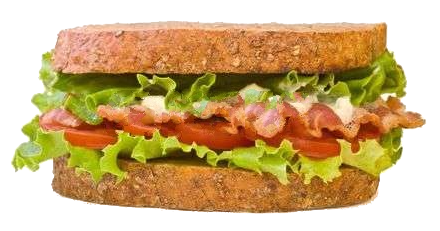
\includegraphics[scale=0.12]{graphics/blt}\end{tikzpicture}} theorem.

\bl
Let $(V,\|\cdot\|)$ be a normed space and let $\mathcal{D}_A$ be a dense subspace of $V$. Then, for any $f\in V$, there exists a sequence $\{\alpha_n\}_{n\in \N}$ in $\mathcal{D}_A$ which converges to $f$.
\el
\bq
Let $f\in V$. Clearly, there exists a sequence $\{f_n\}_{n\in \N}$ in $V$ which converges to $f$ (for instance, the constant sequence). Let $\varepsilon >0$. Then, there exists $N\in \N$ such that
\bse
\forall \, n\geq N : \ \|f_n-f\| < \tfrac{\varepsilon}{2}.
\ese
Since $\mathcal{D}_A$ is dense in $V$ and each $f_n\in V$, we have
\bse
\forall \, n\in \N : \exists\, \alpha_n\in\mathcal{D}_A : \ \|\alpha_n-f_n\|<\tfrac{\varepsilon}{2}.\\[8pt]
\ese
The sequence $\{\alpha_n\}_{n\in \N}$ is a sequence in $\mathcal{D}_A$ and we have
\bi{rCl}
\|\alpha_n-f\|&=&\|\alpha_n-f_n+f_n-f\|\\
&\leq &\|\alpha_n-f_n\|+\|f_n-f\| \\
&<&\tfrac{\varepsilon}{2}+\tfrac{\varepsilon}{2}\\
&=&\varepsilon
\ei
for all $n\geq N$. Hence $\displaystyle \lim_{n\to\infty}\alpha_n=f$.
\eq

\bd
Let $V,W$ be vector spaces and let $A\cl\mathcal{D}_A\to W$ be a linear map, where $\mathcal{D}_A\subseteq V$. An \emph{extension}\index{extension} of $A$ is a linear map $\widehat A\cl V\to W$ such that
\bse
\forall \, \alpha\in \mathcal{D}_A : \ \widehat A \alpha = A\alpha.
\ese
\ed

\bt[BLT theorem]
Let $V$ be a normed space and $W$ a Banach space. Any densely defined linear map $A\cl\mathcal{D}_A\to W$ has a unique extension $\widehat A\cl V\to W$ such that $\widehat A$ is bounded. Moreover, $\|{\widehat A}\|=\|A\|$.
\et

\bq
\ben[label=(\alph*)]
\item Let $A\in \mathcal{L}(\mathcal{D}_A,W)$. Since $\mathcal{D}_A$ is dense in $V$, for any $f\in V$ there exists a sequence $\{\alpha_n\}_{n\in \N}$ in $\mathcal{D}_A$ which converges to $f$. Moreover, since $A$ is bounded, we have 
\bse
\forall \, n\in \N : \ \|A\alpha_n-A\alpha_m\|_W \leq \|A\| \|\alpha_n-\alpha_m\|_V,
\ese
from which it quickly follows that $\{A\alpha_n\}_{n\in \N}$ is Cauchy in $W$. As $W$ is a Banach space, this sequence converges to an element of $W$ and thus we can define
\bi{rrCl}
\widehat A \cl & V &\to & W\\
& f & \mapsto & \lim_{n\to\infty}A\alpha_n,
\ei
where $\{\alpha_n\}_{n\in \N}$ is any sequence in $\mathcal{D}_A$ which converges to $f$.
\item First, let us show that $\widehat A$ is well-defined. Let $\{\alpha_n\}_{n\in \N}$ and $\{\beta_n\}_{n\in \N}$ be two sequences in $\mathcal{D}_A$ which converge to $f\in V$ and let $\varepsilon > 0$. Then, there exist $N_1,N_2\in \N$ such that
\bi{c}
\forall \, n\geq N_1 : \ \|\alpha_n-f\|_V < \frac{\varepsilon}{2\|A\|}\\
\forall \, n\geq N_2 : \ \|\beta_n-f\|_V < \frac{\varepsilon}{2\|A\|}.
\ei
Let $N:=\max\{N_1,N_2\}$. Then, for all $n\geq N$, we have
\bi{rCl}
\|A\alpha_n-A\beta_n\|_W & = & \|A(\alpha_n-\beta_n)\|_W\\
&\leq & \|A\| \| \alpha_n-\beta_n\|_V\\
& = & \|A\| \| \alpha_n-f+f-\beta_n\|_V\\
&\leq & \|A\| (\| \alpha_n-f\|_V+\|f-\beta_n\|_V)\\
&< & \|A\| \Bigl(\frac{\varepsilon}{2\|A\|}+\frac{\varepsilon}{2\|A\|}\Bigr)\\
&=&\varepsilon,
\ei
where we have used the fact that $A$ is bounded. Thus, we have shown
\bse
\lim_{n\to\infty}(A\alpha_n-A\beta_n) = 0.
\ese
Then, by using \Cref{lem:forcompl} and rearranging, we find
\bse
\lim_{n\to\infty}A\alpha_n = \lim_{n\to\infty}A\beta_n,
\ese
that is, $\widehat A$ is indeed well-defined.

\item To see that $\widehat A$ is an extension of $A$, let $\alpha\in\mathcal{D}_A$. The constant sequence $\{\alpha_n\}_{n\in \N}$ with $\alpha_n=\alpha$ for all $n\in \N$ is a sequence in $\mathcal{D}_A$ converging to $\alpha$. Hence
\bse
\widehat A \alpha := \lim_{n\to\infty} A\alpha_n =  \lim_{n\to\infty} A\alpha = A\alpha.
\ese

\item We now check that $A\in\mathcal{L}(V,W)$. For linearity, let $f,g\in V$ and $z\in \C$. As $\mathcal{D}_A$ is dense in $V$, there exist sequences $\{\alpha_n\}_{n\in \N}$ and $\{\beta_n\}_{n\in \N}$ in $\mathcal{D}_A$ converging to $f$ and $g$, respectively. Moreover, as $\mathcal{D}_A$ is a subspace of $V$, the sequence $\{\gamma_n\}_{n\in \N}$ given by
\bse
\gamma_n:=z\alpha_n+\beta_n
\ese
is again a sequence in $\mathcal{D}_A$ and, by \Cref{lem:forcompl}, 
\bse
\lim_{n\to\infty}\gamma_n = zf+g.
\ese
Then, we have
\bi{rCl}
\widehat A (zf+g) &:=& \lim_{n\to\infty} A\gamma_n \\
&=& \lim_{n\to\infty}A(z\alpha_n+\beta_n)\\
&=& \lim_{n\to\infty}(zA\alpha_n+A\beta_n)\\
&=& z\lim_{n\to\infty}A\alpha_n+\lim_{n\to\infty}A\beta_n\\
&=:& z\widehat A f+\widehat Ag .
\ei
For boundedness, let $f\in V$ and $\{\alpha_n\}_{n\in \N}$ a sequence in $\mathcal{D}_A$ which converges to $f$. Then, since $A$ is bounded,
\bi{rCl}
\|\widehat A f\|_W &:=& \bigl\|\lim_{n\to\infty}A\alpha_n\bigr\|_W\\
 &=& \lim_{n\to\infty}\|A\alpha_n\|_W\\
 & \leq &\lim_{n\to\infty}\|A\|\|\alpha_n\|_V\\
 & = &\|A\|\lim_{n\to\infty}\|\alpha_n\|_V\\
 & = &\|A\|\|f\|_V.
\ei
Therefore
\bse
\sup_{f\in V} \frac{\|\widehat A f\|_W}{\|f\|_V} \leq \sup_{f\in V} \frac{\|A\|\|f\|_V}{\|f\|_V} =\sup_{f\in V} \|A\| =\|A\| < \infty
\ese
and hence $\widehat A$ is bounded.
\item For uniqueness, suppose that $\widetilde A\in\mathcal{L}(V,W)$ is another extension of $A$. Let $f\in V$ and $\{\alpha_n\}_{n\in \N}$ a sequence in $\mathcal{D}_A$ which converges to $f$. Then, we have
\bse
\|\widetilde A f - A\alpha_n\|_W = \|\widetilde A f - \widetilde A\alpha_n\|_W \leq  \|\widetilde A\| \|f-\alpha_n\|_V .
\ese
It follows that
\bse
\lim_{n\to\infty}(\widetilde A f - A\alpha_n) = 0
\ese
and hence, for all $f\in V$,
\bse
\widetilde Af = \lim_{n\to\infty} A\alpha_n =: \widehat A f.
\ese
Therefore, $\widetilde A = \widehat A$.
\item Finally, we have already shown in part (d) that
\bse
\|\widehat A\|:=\sup_{f\in V} \frac{\|\widehat A f\|_W}{\|f\|_V} \leq \|A\|.
\ese
On the other hand, since $\mathcal{D}_A\subseteq V$, we must also have
\bse
\|A\|:=\sup_{f\in \mathcal{D}_A} \frac{\| A f\|_W}{\|f\|_V} = \sup_{f\in \mathcal{D}_A} \frac{\|\widehat A f\|_W}{\|f\|_V} \leq \sup_{f\in V} \frac{\|\widehat A f\|_W}{\|f\|_V}=: \|\widehat A\|.
\ese
Hence, we also have $\|A\|\leq\|\widehat A\|$. Thus, $\|\widehat A\|=\|A\|$.\qedhere
\een
\eq

\br
Note a slight abuse of notation in the equality $\|\widehat A\|=\|A\|$. The linear maps $\widehat A$ and $A$ belong to $\mathcal{L}(V,W)$ and $\mathcal{L}(\mathcal{D}_A,W)$, respectively. These are different normed (in fact, Banach) spaces and, in particular, carry \emph{different} norms. To be more precise, we should have written
\bse
\|\widehat A\|_{\mathcal{L}(V,W)} = \|A\|_{\mathcal{L}(\mathcal{D}_A,W)},
\ese
where 
\bse
\|\widehat A\|_{\mathcal{L}(V,W)} := \sup_{f\in V} \frac{\| \widehat A f\|_W}{\|f\|_V} \qquad \text{and}\qquad
\| A\|_{\mathcal{L}(\mathcal{D}_A,W)} := \sup_{f\in \mathcal{D}_A} \frac{\| A f\|_W}{\|f\|_V}.
\ese
\er






















\newpage

\section{Separable Hilbert Spaces}


\subsection{Relationship between norms and inner products}

A Hilbert space is a vector space $(\mathcal{H},+,\cdot)$ equipped with a sesqui-linear inner product $\langle\cdot|\cdot\rangle$ which induces a norm $\|\cdot\|_{\mathcal{H}}$ with respect to which $\mathcal{H}$ is a Banach space. Note that by ``being induced by $\langle\cdot|\cdot\rangle$'' we specifically mean that the norm is defined as
\bi{rrCl}
\|\cdot\|\cl & V & \to & \R\\
& f & \mapsto & \sqrt{\langle f|f\rangle}.
\ei

Recall that a sesqui-linear inner product on $\mathcal{H}$ is a map $\langle\cdot|\cdot\rangle\cl \mathcal{H} \times \mathcal{H} \to \C$ which is conjugate symmetric, linear in the second argument and positive-definite. Note that conjugate symmetry together with linearity in the second argument imply conjugate linearity in the first argument:
\bi{rCl}
\langle z\psi_1+\psi_2|\varphi\rangle & = & \overline{\langle \varphi| z\psi_1+\psi_2\rangle }\\
& = & \overline{z\langle \varphi| \psi_1\rangle+\langle \varphi| \psi_2\rangle }\\
& = & \overline{z}\overline{\langle \varphi| \psi_1\rangle}+\overline{\langle \varphi| \psi_2\rangle }\\
& = & \overline{z}\langle \psi_1|\varphi\rangle+\langle \psi_2|\varphi\rangle .
\ei

Of course, since Hilbert spaces are a special case of Banach spaces, everything that we have learned about Banach spaces also applies to Hilbert paces. For instance, $\mathcal{L}(\mathcal{H},\mathcal{H})$, the collection of all bounded linear maps $\mathcal{H}\to \mathcal{H}$, is a Banach space with respect to the operator norm. In particular, the dual of a Hilbert space $\mathcal{H}$ is just $\mathcal{H}^*:=\mathcal{L}(\mathcal{H},\C)$.
We will see that the operator norm on $\mathcal{H}^*$ is such that there exists an inner product on $\mathcal{H}^*$ which induces it, so that the dual of a Hilbert space is again a Hilbert space.

First, in order to check that the norm induced by an inner product on $V$ is indeed a norm on $V$, we need one of the most important inequalities in mathematics.

\bp[Cauchy-Schawrz inequality\footnote{Also known as the Cauchy-Bunyakovsky-Schwarz inequality in the Russian literature.}]\index{Cauchy-Schawrz inequality}
Let $\langle\cdot|\cdot\rangle$ be a sesqui-linear inner product on $V$. Then, for any $f,g \in V$, we have
\bse
|\langle f|g\rangle|^2\leq \langle f|f\rangle \langle g|g\rangle .
\ese
\ep
\bq
If $f=0$ or $g=0$, then equality holds. Hence suppose that $f\neq 0$ and let
\bse
z:= \frac{\langle f|g\rangle}{\langle f|f\rangle} \in \C.
\ese
Then, by positive-definiteness of $\langle\cdot|\cdot\rangle$, we have
\bi{rCl}
0 & \leq & \langle zf-g|zf-g\rangle\\
&  = & |z|^2\langle f|f\rangle -\overline{z}\langle f|g\rangle-z\langle g|f\rangle+\langle g|g\rangle\\
&  = & \frac{|\langle f|g\rangle|^2}{\langle f|f\rangle^2}\langle f|f\rangle -\frac{\,\overline{\langle f|g\rangle}\,}{\langle f|f\rangle}\langle f|g\rangle-\frac{\langle f|g\rangle}{\langle f|f\rangle}\overline{\langle f|g\rangle}+\langle g|g\rangle\\
&  = & \frac{|\langle f|g\rangle|^2}{\langle f|f\rangle} -\frac{|\langle f|g\rangle|^2}{\langle f|f\rangle} -\frac{|\langle f|g\rangle|^2}{\langle f|f\rangle} +\langle g|g\rangle\\
&  = & -\frac{|\langle f|g\rangle|^2}{\langle f|f\rangle} +\langle g|g\rangle.
\ei
By rearranging, since $\langle f | f \rangle >0$, we obtain the desired inequality.
\eq
Note that, by defining $\|f\|:=\sqrt{\langle f | f \rangle }$, and using the fact that $|\la f|g\ra | \geq 0$, we can write the Cauchy-Schwarz inequality as
\bse
|\langle f | g \rangle | \leq \|f\|\|g\|.
\ese
\bp
The induced norm\index{induced norm} on $V$ is a norm.
\ep
\bq
Let $f,g\in V$ and $z\in \C$. Then
\ben[label=(\roman*)]
\item $\|f\|:= \sqrt{\langle f|f\rangle} \geq 0$
\item $\|f\|=0\ \Leftrightarrow\ \|f\|^2=0\ \Leftrightarrow\ \langle f|f\rangle = 0\ \Leftrightarrow\ f =0$ by positive-definiteness
\item $\|zf\|:= \sqrt{\langle zf|zf\rangle} = \sqrt{z\overline{z}\langle f|f\rangle} = \sqrt{|z|^2\langle f|f\rangle}=|z|\sqrt{\langle f|f\rangle}=:|z|\|f\|$
\item Using the fact that $z+\overline{z} = 2\Re z$ and $\Re z\leq |z|$ for any $z\in \C$ and the Cauchy-Schwarz inequality, we have 
\bi{rCl}
\|f+g\|^2 & := & \langle f+g|f+g\rangle\\
& = & \langle f|f\rangle +\langle f|g\rangle+\langle g|f\rangle+\langle g|g\rangle\\
& = & \langle f|f\rangle +\langle f|g\rangle+\overline{\langle f|g\rangle}+\langle g|g\rangle\\
& = & \langle f|f\rangle +2\Re\langle f|g\rangle+\langle g|g\rangle\\
& \leq & \langle f|f\rangle +2|\langle f|g\rangle|+\langle g|g\rangle\\
& \leq & \langle f|f\rangle +2\|f\|\|g\|+\langle g|g\rangle\\
& = & (\|f\|+\|g\|)^2.
\ei
By taking the square root of both sides, we have $\|f+g\|\leq \|f\|+\|g\|$. \qedhere
\een
\eq

Hence, we see that any inner product space (i.e.\ a vector space equipped with a sesqui-linear inner product) is automatically a normed space under the induced norm. It is only natural to wonder whether the converse also holds, that is, whether every norm is induced by some sesqui-linear inner product. Unfortunately, the answer is negative in general. The following theorem gives a necessary and sufficient condition for a norm to be induced by a sesqui-linear inner product and, in fact, by a unique such.

\bt[Jordan-von Neumann]\index{Jordan-von Neumann theorem}
Let $V$ be a vector space. A norm $\|\cdot\|$ on $V$ is induced by a sesqui-linear inner product $\langle\cdot|\cdot\rangle$ on $V$ if, and only if, the parallelogram identity\index{parallelogram identity}
\bse
\|f+g\|^2+\|f-g\|^2=2\|f\|^2+2\|g\|^2
\ese
holds for all $f,g\in V$, in which case, $\langle\cdot|\cdot\rangle$ is determined by the polarisation identity\index{polarisation identity}
\bi{rCl}
\langle f  |  g\rangle & = & \frac{1}{4} \sum_{k=0}^3\mathrm{i}^k\|f+\mathrm{i}^{4-k}g\|^2\\
& = & \frac{1}{4} (\|f+g\|^2-\|f-g\|^2+\mathrm{i}\|f-\mathrm{i}g\|^2 -\mathrm{i}\|f+\mathrm{i}g\|^2).
\ei
\et

\bq
\begin{itemize}
\item[($\Rightarrow$)] If $\|\cdot\|$ is induced by $\langle\cdot|\cdot\rangle$, then by direct computation
\bi{rCl}
\|f+g\|^2+\|f-g\|^2 & := & \langle f+g|f+g\rangle + \langle f-g|f-g\rangle\\
& = & \langle f|f\rangle +\langle f|g\rangle+\langle g|f\rangle+\langle g|g\rangle\\
&  & \negmedspace {} + \langle f|f\rangle -\langle f|g\rangle-\langle g|f\rangle+\langle g|g\rangle\\
& = & 2\langle f|f\rangle + 2\langle g|g\rangle\\
& =: & 2\|f\|^2+2\|g\|^2,
\ei
so the parallelogram identity is satisfied. We also have
\bi{rCl}
\|f+g\|^2-\|f-g\|^2 & := & \langle f+g|f+g\rangle - \langle f-g|f-g\rangle\\
& = & \langle f|f\rangle +\langle f|g\rangle+\langle g|f\rangle+\langle g|g\rangle\\
&  & \negmedspace {} - \langle f|f\rangle +\langle f|g\rangle+\langle g|f\rangle-\langle g|g\rangle\\
& = & 2\langle f|g\rangle+2\langle g|f\rangle
\ei
and
\bi{rCl}
\mathrm{i}\|f-\mathrm{i}g\|^2-\mathrm{i}\|f+\mathrm{i}g\|^2 & := & \mathrm{i}\langle f-\mathrm{i}g|f-\mathrm{i}g\rangle - \mathrm{i}\langle f+\mathrm{i}g|f+\mathrm{i}g\rangle\\
& = & \mathrm{i}\langle f|f\rangle +\langle f|g\rangle-\langle g|f\rangle+\mathrm{i}\langle g|g\rangle\\
&  & \negmedspace {} - \mathrm{i} \langle f|f\rangle +\langle f|g\rangle-\langle g|f\rangle-\mathrm{i}\langle g|g\rangle\\
& = & 2\langle f|g\rangle-2\langle g|f\rangle.
\ei
Therefore
\bse
\|f+g\|^2-\|f-g\|^2+\mathrm{i}\|f-\mathrm{i}g\|^2 -\mathrm{i}\|f+\mathrm{i}g\|^2 = 4\langle f|g\rangle.
\ese
that is, the inner product is determined by the polarisation identity. 
\item[($\Leftarrow$)] Suppose that $\|\cdot\|$ satisfies the parallelogram identity. Define $\langle\cdot|\cdot\rangle$ by
\bse
\langle f  |  g\rangle := \frac{1}{4} (\|f+g\|^2-\|f-g\|^2+\mathrm{i}\|f-\mathrm{i}g\|^2-\mathrm{i}\|f+\mathrm{i}g\|^2).
\ese
We need to check that this satisfies the defining properties of a sesqui-linear inner product.
\ben[label=(\roman*)]
\item For conjugate symmetry
\bi{rCl}
\overline{\langle f  |  g\rangle} & := & \tfrac{1}{4} \bigl(\,\overline{\|f+g\|^2-\|f-g\|^2+\mathrm{i}\|f-\mathrm{i}g\|^2-\mathrm{i}\|f+\mathrm{i}g\|^2}\,\bigr)\\
& = & \tfrac{1}{4} (\|f+g\|^2-\|f-g\|^2-\mathrm{i}\|f-\mathrm{i}g\|^2+\mathrm{i}\|f+\mathrm{i}g\|^2)\\
& = & \tfrac{1}{4} (\|f+g\|^2-\|f-g\|^2-\mathrm{i}\|(-\mathrm{i})(\mathrm{i}f+g)\|^2+\mathrm{i}\|\mathrm{i}(-\mathrm{i}f+g)\|^2)\\
& = & \tfrac{1}{4} (\|g+f\|^2-\|g-f\|^2-\mathrm{i}(|-\mathrm{i}|)^2\|g+\mathrm{i}f\|^2+\mathrm{i}(|\mathrm{i}|)^2\|g-\mathrm{i}f\|^2)\\
& = & \tfrac{1}{4} (\|g+f\|^2-\|g-f\|^2-\mathrm{i}\|g+\mathrm{i}f\|^2+\mathrm{i}\|g-\mathrm{i}f\|^2)\\
& =: & \langle g | f \rangle
\ei

\item We will now show linearity in the second argument. This is fairly non-trivial and quite lengthy. %\footnote{We adapt and take inspiration from answers to a question on \href{https://math.stackexchange.com/questions/21792/norms-induced-by-inner-products-and-the-parallelogram-law}{Math.StackExhange}.}
We will focus on additivity first. We have
\bi{c}
\langle f | g+h \rangle  :=  \frac{1}{4} (\|f+g+h\|^2-\|f-g-h\|^2+\mathrm{i}\|f-\mathrm{i}g-\mathrm{i}h\|^2-\mathrm{i}\|f+\mathrm{i}g+\mathrm{i}h\|^2).
\ei
Consider the real part of $\langle f | g+h \rangle $. By successive applications of the parallelogram identity, we find
\bi{rCl}
\Re\langle f | g + h \rangle & = & \tfrac{1}{4} (\|f+g+h\|^2-\|f-g-h\|^2)\\
& = & \tfrac{1}{4} (\|f+g+h\|^2+\|f+g-h\|^2-\|f+g-h\|^2-\|f-g-h\|^2)\\
& = & \tfrac{1}{4} (2\|f+g\|^2+2\|h\|^2-2\|f-h\|^2-2\|g\|^2)\\
& = & \tfrac{1}{4} (2\|f+g\|^2+2\|f\|^2+2\|h\|^2-2\|f-h\|^2-2\|f\|^2-2\|g\|^2)\\
& = & \tfrac{1}{4} (2\|f+g\|^2+\|f+h\|^2+\|f-h\|^2-2\|f-h\|^2-\|f+g\|^2-\|f-g\|^2)\\
& = & \tfrac{1}{4} (\|f+g\|^2+\|f+h\|^2-\|f-h\|^2-\|f-g\|^2)\\
& = & \Re\langle f | g  \rangle+\Re\langle f | h \rangle.
\ei
Replacing $g$ and $h$ with $-\mathrm{i}g$ and $-\mathrm{i}h$ respectively, we obtain
\bse
\Im \langle f | g + h \rangle = \Im\langle f | g  \rangle+\Im\langle f | h \rangle.
\ese
Hence, we have
\bi{rCl}
\langle f | g + h \rangle & = & \Re\langle f | g + h \rangle+\mathrm{i}\Im\langle f | g + h \rangle\\
& = & \Re\langle f | g  \rangle+\Re\langle f | h \rangle+\mathrm{i}(\Im\langle f | g  \rangle+\Im\langle f | h \rangle)\\
& = & \Re\langle f | g  \rangle+\mathrm{i}\Im\langle f | g  \rangle +\Re\langle f | h \rangle+\mathrm{i}\Im\langle f | h \rangle\\
& = & \langle f | g  \rangle+\langle f | h \rangle,
\ei
which proves additivity.

For scaling invariance, we will proceed in several steps.
\ben[label=(\alph*)]
\item First, note that
\bse
\langle f | 0 \rangle := \tfrac{1}{4} (\|f\|^2-\|f\|^2+\mathrm{i}\|f\|^2-\mathrm{i}\|f\|^2) = 0
\ese
and hence $\langle f | 0g \rangle = 0\langle f | g \rangle$ holds.
\item Suppose that $\langle f | ng \rangle = n\langle f | g \rangle$ for some $n\in \N$. Then, by additivity
\bi{rCl}
\langle f | (n+1)g \rangle & = & \langle f | ng+g \rangle\\
& = & \langle f | ng \rangle + \langle f | g \rangle\\
& = & n\langle f | g \rangle + \langle f | g \rangle\\
& = & (n+1)\langle f | g \rangle.
\ei
Hence, by induction on $n$ with base case (a), we have
\bse
\forall \, n \in \N : \ \langle f | ng \rangle = n\langle f | g \rangle.
\ese
\item Note that by additivity
\bse
\langle f | g \rangle + \langle f | {-g} \rangle = \langle f | g -g\rangle = \langle f | 0 \rangle \stackrel{(\mathrm{a})}{=} 0.
\ese
Hence $\langle f | {-g} \rangle = -\langle f | g \rangle$.
\item Then, for any $n\in \N$
\bse
\langle f | {-ng} \rangle \stackrel{(\mathrm{c})}{=} -\langle f | ng \rangle \stackrel{(\mathrm{b})}{=} -n\langle f | g \rangle
\ese
and thus
\bse
\forall \, n \in \Z : \ \langle f | ng \rangle = n\langle f | g \rangle.
\ese
\item Now note that for any $m\in \Z\setminus\{0\}$
\bse
m\langle f | \tfrac{1}{m}g \rangle \stackrel{(\mathrm{d})}{=} \langle f | m\tfrac{1}{m} g \rangle = \langle f | g \rangle
\ese
and hence, by dividing by $m$, we have $\langle f | \frac{1}{m} g \rangle = \frac{1}{m}\langle f | g \rangle$.
\item Therefore, for any $r=\tfrac{n}{m}\in \Q$, we have
\bse
\langle f | r g \rangle = \langle f | \tfrac{n}{m} g \rangle \stackrel{(\mathrm{d})}{=}  n\langle f | \tfrac{1}{m}g \rangle \stackrel{(\mathrm{e})}{=}  \tfrac{n}{m}\langle f | g \rangle = r\langle f | g \rangle
\ese
and hence
\bse
\forall \, r \in \Q : \ \langle f | rg \rangle = r\langle f | g \rangle.
\ese
\item Before we turn to $\R$, we need to show that $|\langle f | g \rangle | \leq \sqrt{2}\|f\|\|g\|$. Note that here we \emph{cannot} invoke the Cauchy-Schwarz inequality (which would also provide a better estimate) since we don't know that $\langle \cdot | \cdot \rangle$ is an inner product yet. First, consider the real part of $\langle f | g \rangle$.
\bi{rCl}
\Re \langle f | g \rangle & = & \tfrac{1}{4} (\|f+g\|^2-\|f-g\|^2)\\
& = &  \tfrac{1}{4} (2\|f+g\|^2-\|f+g\|^2-\|f-g\|^2)\\
& = &  \tfrac{1}{4} (2\|f+g\|^2-2\|f\|^2-2\|g\|^2)\\
& \leq &  \tfrac{1}{4} (2(\|f\|+\|g\|)^2-2\|f\|^2-2\|g\|^2)\\
& = &  \tfrac{1}{4} (2\|f\|^2+4\|f\|\|g\|+2\|g\|^2-2\|f\|^2-2\|g\|^2)\\
& = &  \|f\|\|g\|.
\ei
Replacing $g$ with $-\mathrm{i}g$ and noting that $\|-\mathrm{i}g\|=|-\mathrm{i}|\|g\|=\|g\|$, we also have 
\bse
\Im \langle f | g \rangle \leq \|f\|\|g\|.
\ese
Hence, we find
\bi{rCl}
| \langle f | g \rangle | & = & |\Re \langle f | g \rangle+\mathrm{i}\Im \langle f | g \rangle|\\
& = & \sqrt{(\Re \langle f | g \rangle)^2+(\Im \langle f | g \rangle)^2}\\
& \leq & \sqrt{(\|f\|\|g\|)^2+(\|f\|\|g\|)^2}\\
& = &  \sqrt{2}\|f\|\|g\|.
\ei

\item Let $r\in \R$. Since $\R$ is the completion of $\Q$ (equivalently, $\Q$ is dense in $\R$), there exists a sequence $\{r_n\}_{n\in\N}$ in $\Q$ which converges to $r$. Let $\varepsilon >0$. Then, there exist $N_1,N_2\in\N$ such that
\bi{rCl}
\forall \, n \geq N_1 &:& \ |r_n-r|<\frac{\varepsilon}{2\sqrt{2}\|f\|\|g\|}\\
\forall \, n,m \geq N_2 &:& \ |r_n-r_m|<\frac{\varepsilon}{2\sqrt{2}\|f\|\|g\|}.
\ei
Let $N:=\max\{N_1,N_2\}$ and fix $m\geq N$. Then, for all $n\geq N$, we have
\bi{rCl}
| r_n\langle f | g \rangle - \langle f | rg \rangle | & = & | r_n\langle f | g \rangle - r_m\langle f | g \rangle+ r_m\langle f | g \rangle- \langle f | rg \rangle | \\
 & \stackrel{(\mathrm{f})}{=} & | r_n\langle f | g \rangle - r_m\langle f | g \rangle+ \langle f | r_m g \rangle- \langle f | rg \rangle | \\
 & = & | (r_n-r_m)\langle f | g \rangle + \langle f | (r_m-r) g \rangle | \\
 & \leq & | (r_n-r_m)\langle f | g \rangle | + | \langle f | (r_m-r) g \rangle | \\
 & \stackrel{(\mathrm{g})}{\leq} & \sqrt{2}|r_n-r_m| \| f \| \| g \| + \sqrt{2}\| f \| \| (r_m-r)g \| \\
 & = & \sqrt{2}|r_n-r_m| \| f \| \| g \| + \sqrt{2}|r_m-r|\| f \| \| g \| \\
 & < & \sqrt{2} \frac{\varepsilon}{2\sqrt{2}\|f\|\|g\|} \| f \| \| g \| +  \sqrt{2} \frac{\varepsilon}{2\sqrt{2}\|f\|\|g\|} \| f \| \| g \|\\
& = & \varepsilon,
\ei
that is, $\displaystyle \lim_{n\to\infty} r_n \langle f | g \rangle = \langle f | rg \rangle$.

\item Hence, for any $r\in \R$, we have
\bse
r\langle f | g \rangle = \bigl(\lim_{\,n\to\infty}r_n\bigr) \langle f | g \rangle = \lim_{n\to\infty} r_n \langle f | g \rangle \stackrel{(\mathrm{h})}{=} \langle f | rg \rangle  
\ese
and thus
\bse
\forall \, r \in \R : \ r\langle f | g \rangle = \langle f | rg \rangle  .
\ese

\item We now note that
\bi{rCl}
\langle f  | \mathrm{i} g\rangle & := & \tfrac{1}{4} (\|f+\mathrm{i}g\|^2-\|f-\mathrm{i}g\|^2+\mathrm{i}\|f-\mathrm{i}^2g\|^2-\mathrm{i}\|f+\mathrm{i}^2g\|^2)\\
& = & \tfrac{1}{4} \mathrm{i} \, (-\mathrm{i}\|f+\mathrm{i}g\|^2+\|f-\mathrm{i}g\|^2+\mathrm{i}\|f+g\|^2-\|f-g\|^2)\\
& =: & \mathrm{i}\langle f  | g\rangle
\ei
and hence $ \langle f  | \mathrm{i} g\rangle= \mathrm{i}\langle f  | g\rangle$.

\item Let $z\in \C$. By additivity, we have
\bi{rCl}
\langle f  | z g\rangle & = & \langle f  | (\Re z + \mathrm{i}\Im z) g\rangle\\
& = & \langle f  | (\Re z) g\rangle+ \langle f  | \mathrm{i}(\Im z )g\rangle\\
& \stackrel{(\mathrm{j})}{=} & \langle f  | (\Re z) g\rangle+ \mathrm{i}\langle f  | (\Im z) g\rangle\\
& \stackrel{(\mathrm{i})}{=} & \Re z\langle f  | g\rangle+ \mathrm{i}\Im z \langle f  |  g\rangle\\
& = & (\Re z+ \mathrm{i}\Im z)\langle f  |  g\rangle\\
& = & z\langle f  |  g\rangle,
\ei
which shows scaling invariance in the second argument.
\een
Combining additivity and scaling invariance in the second argument yields linearity in the second argument.
\item For positive-definiteness
\bi{rCl}
\langle f | f \rangle & := & \tfrac{1}{4} (\|f+f\|^2-\|f-f\|^2+\mathrm{i}\|f-\mathrm{i}f\|^2-\mathrm{i}\|f+\mathrm{i}f\|^2)\\
& = & \tfrac{1}{4} (4\|f\|^2+\mathrm{i}|1-\mathrm{i}|^2\|f\|^2-\mathrm{i}|1+\mathrm{i}|^2\|f\|^2)\\
& = & \tfrac{1}{4} (4+\mathrm{i}|1-\mathrm{i}|^2-\mathrm{i}|1+\mathrm{i}|^2)\|f\|^2\\
& = & \tfrac{1}{4} (4+2\mathrm{i}-2\mathrm{i})\|f\|^2\\
& = & \|f\|^2.
\ei
Thus, $\langle f | f \rangle\geq 0$ and $\langle f | f \rangle = 0 \ \Leftrightarrow \ f=0$.
\een
Hence, $\langle \cdot| \cdot \rangle$ is indeed a sesqui-linear inner product. Note that, from part (iii) above, we have
\bse
\sqrt{\langle f | f \rangle}=\|f\|.
\ese
That is, the inner product $\langle \cdot| \cdot \rangle$ does induce the norm from which we started, and this completes the proof.\qedhere
\end{itemize}
\eq

\br
Our proof of linearity is based on the hints given in Section 6.1, Exercise 27, from \textit{Linear Algebra} (4th Edition) by Friedberg, Insel, Spence. Other proofs of the Jordan-von Neumann theorem can be found in
\begin{itemize}
\item Kadison, Ringrose, \textit{Fundamentals of the Theory of Operator Algebras: Volume I: Elementary Theory}, American Mathematical Society 1997
\item Kutateladze, \textit{Fundamentals of Functional Analysis}, Springer 1996.
\item Day, \textit{Normed Linear Spaces}, Springer 1973.
\end{itemize}
\er

\br
Note that, often in the more mathematical literature, a sesqui-linear inner product is defined to be linear in the \emph{first} argument rather than the second. In that case, the polarisation identity takes the form
\bi{rCl}
\langle f  |  g\rangle & = & \frac{1}{4} \sum_{k=0}^3\mathrm{i}^k\|f+\mathrm{i}^{k}g\|^2\\
& = & \frac{1}{4} (\|f+g\|^2-\|f-g\|^2+\mathrm{i}\|f+\mathrm{i}g\|^2 -\mathrm{i}\|f-\mathrm{i}g\|^2).
\ei
\er

\be
Consider $C_{\C}^0[0,1]$ and let $f(x)=x$ and $g(x)=1$. Then
\bse
\|f\|_{\infty} = 1, \qquad \|g\|_{\infty} = 1, \qquad \|f+g\|_{\infty}=2,\qquad \|f-g\|_{\infty}=1
\ese
and hence
\bse
\|f+g\|_{\infty}^2+ \|f-g\|^2_{\infty}=5\neq 4 =2\|f\|_{\infty}^2  +2 \|g\|_{\infty}^2.
\ese
Thus, by the Jordan-von Neumann theorem, there is no inner product on $C_{\C}^0[0,1]$ which induces the supremum norm. Therefore, $(C_{\C}^0[0,1],\|\cdot\|_{\infty})$ cannot be a Hilbert space.
\ee

\bp
Let $\mathcal{H}$ be a Hilbert space. Then, $\mathcal{H}^*$ is a Hilbert space.
\ep
\bq
We already know that $\mathcal{H}^*:=\mathcal{L}(\mathcal{H},\C)$ is a Banach space. The norm on $\mathcal{H}^*$ is just the usual operator norm
\bse
\|f\|_{\mathcal{H}^*}:=\sup_{\varphi\in\mathcal{H}}\frac{|f(\varphi)|}{\|\varphi\|_{\mathcal{H}}}
\ese
where, admittedly somewhat perversely, we have reversed our previous notation for the dual elements. Since the modulus is induced by the standard inner product on $\C$, i.e.\ $|z|=\sqrt{z\overline{z}}$, it satisfies the parallelogram identity. Hence, we have
\bi{rCl}
\|f+g\|^2_{\mathcal{H}^*}+\|f-g\|^2_{\mathcal{H}^*} & := &\biggl(\sup_{\,\varphi\in\mathcal{H}}\frac{|(f+g)(\varphi)|}{\|\varphi\|_{\mathcal{H}}}\biggr)^{\negmedspace 2} +\biggl(\sup_{\,\varphi\in\mathcal{H}}\frac{|(f-g)(\varphi)|}{\|\varphi\|_{\mathcal{H}}}\biggr)^{\negmedspace 2} \\
 & = &\sup_{\varphi\in\mathcal{H}}\frac{|(f+g)(\varphi)|^2}{\|\varphi\|^2_{\mathcal{H}}} +\sup_{\varphi\in\mathcal{H}}\frac{|(f-g)(\varphi)|^2}{\|\varphi\|^2_{\mathcal{H}}} \\
& = & \sup_{\varphi\in\mathcal{H}}\frac{|f(\varphi)+g(\varphi)|^2+|f(\varphi)-g(\varphi)|^2}{\|\varphi\|^2_{\mathcal{H}}} \\
& = & \sup_{\varphi\in\mathcal{H}}\frac{2|f(\varphi)|^2+2|g(\varphi)|^2}{\|\varphi\|^2_{\mathcal{H}}} \\
 & = & 2\sup_{\varphi\in\mathcal{H}}\frac{|f(\varphi)|^2}{\|\varphi\|^2_{\mathcal{H}}} +2\sup_{\varphi\in\mathcal{H}}\frac{|g(\varphi)|^2}{\|\varphi\|^2_{\mathcal{H}}} \\
 & =: & 2\|f\|^2_{\mathcal{H}^*}+2\|g\|^2_{\mathcal{H}^*},
\ei
where several steps are justified by the fact that the quantities involved are non-negative. Hence, by the Jordan-von Neumann theorem, the inner product on $\mathcal{H}^*$ defined by the polarisation identity induces $\|\cdot\|_{\mathcal{H}^*}$. Hence, $\mathcal{H}^*$ is a Hilbert space.
\eq

The following useful fact is an immediate application of the Cauchy-Schwarz inequality.

\bp
Inner products on a vector space are sequentially continuous.
\ep

\bq
Let $\langle\cdot|\cdot\rangle$ be an inner product on $V$. Fix $\varphi\in V$ and let $\displaystyle\lim_{n\to \infty}\psi_n=\psi$. Then
\bi{rCl}
|\langle\varphi|\psi_n\rangle-\langle \varphi|\psi\rangle| & = & |\langle\varphi|\psi_n-\psi\rangle|\\
& \leq & \|\varphi\|\|\psi_n-\psi\|
\ei
and hence $\displaystyle\lim_{n\to \infty}\langle\varphi|\psi_n\rangle=\langle\varphi|\psi\rangle$.
\eq


\subsection[Hamel versus Schauder]{Hamel versus Schauder\protect\footnote{\emph{Not} a boxing competition. \begin{tikzpicture}[baseline={($ (current bounding box.center)- (0,-7pt) $)}]
\includegraphics[scale=0.05]{graphics/boxe}\end{tikzpicture} }}

Choosing a basis on a vector space is normally regarded as mathematically inelegant. The reason for this is that most statements about vector spaces are much clearer and, we maintain, aesthetically pleasing when expressed without making reference to a basis. However, in addition to the fact that some statements are more easily and usefully written in terms of a basis, bases provide a convenient way to specify the elements of a vector space in terms of components.
The notion of basis for a vector space that you most probably met in your linear algebra course is more properly know as Hamel basis.

\bd
A \emph{Hamel basis}\index{Hamel basis} of a vector space $V$ is a subset $\mathcal{B}\subseteq V$ such that
\ben[label=(\roman*)]
\item any finite subset $\{e_1,\ldots,e_n\}\subseteq \mathcal{B}$ is \emph{linearly independent}, i.e.\
\bse
\sum_{i=1}^n\lambda^ie_i = 0 \quad \Rightarrow \quad \lambda^1=\cdots = \lambda^n=0
\ese
\item the set $\mathcal{B}$ is a \emph{generating} (or \emph{spanning}) \emph{set} for $V$. That is, for any element $v\in V$, there exist a finite subset $\{e_1,\ldots,e_n\}\subseteq \mathcal{B}$ and $\lambda^1,\ldots,\lambda^n\in\C$ such that
\bse
v = \sum_{i=1}^n\lambda^ie_i.
\ese
Equivalently, by defining the \emph{linear span} of a subset $U\subseteq V$ as
\bse
\lspan U := \biggl\{\sum_{i=1}^n\lambda^iu_i\ \Big|\ \lambda^1,\ldots,\lambda^n\in\C,\, u_1,\ldots,u_n\in U \text{ and } n\geq 1\biggr\},
\ese
i.e.\ the set of all finite linear combinations of elements of $U$ with complex coefficients, we can restate this condition simply as $V = \lspan \mathcal{B}$.
\een
\ed
Given a basis $\mathcal{B}$, one can show that for each $v\in V$ the $\lambda^1,\ldots,\lambda^n$ appearing in (ii) above are uniquely determined. They are called the \emph{components} of $v$ with respect to $\mathcal{B}$. 

One can also show that if a vector space admits a finite Hamel basis $\mathcal{B}$, then any other basis of $V$ is also finite and, in fact, of the same cardinality as $\mathcal{B}$.

\bd
If a vector space $V$ admits a finite Hamel basis, then it is said to be \emph{finite-dimensional} and its \emph{dimension} is $\dim V := |\mathcal{B}|$. Otherwise, it is said to be \emph{infinite-dimensional} and we write $\dim V = \infty$.
\ed

\bt
Every vector space admits a Hamel basis.
\et

For a proof of (a slightly more general version of) this theorem, we refer the interested reader to Dr Schuller's \emph{Lectures on the Geometric Anatomy of Theoretical Physics}.
\medskip


Note that the proof that every vector space admits a Hamel basis relies on the axiom of choice and, hence, it is non-constructive. By a corollary to Baire's category theorem, a Hamel basis on a Banach space is either finite or \emph{uncountably} infinite. Thus, while every Banach space admits a Hamel basis, such bases on infinite-dimensional Banach spaces are difficult to construct explicitly and, hence, not terribly useful to express vectors in terms of components and perform computations. Thankfully, we can use the extra structure of a Banach space to define a more useful type of basis.

\bd
Let $(W,\|\cdot\|)$ be a Banach space. A \emph{Schauder basis}\index{Schauder basis} of $W$ is a sequence $\{e_n\}_{n\in \N}$ in $W$ such that, for any $f\in W$, there exists a unique sequence $\{\lambda^n\}_{n\in \N}$ in $\C$ such that
\bse
f = \lim_{n\to \infty} \sum_{i=0}^n\lambda^ie_i =: \sum_{i=0}^{\infty}\lambda^ie_i
\ese
or, by explicitly using the definition of limit in $W$,
\bse
\lim_{n\to \infty} \, \biggl\|f-\sum_{i=0}^n\lambda^ie_i\biggr\| = 0.
\ese
\ed

\noindent We note the following points.
\begin{itemize}
\item Since Schauder bases require a notion of convergence, they can only be defined on a vector space equipped with a (compatible) topological structure, of which Banach spaces are a special case.
\item Unlike Hamel bases, Schauder bases need not exist.
\item Since the convergence of a series may depend on the order of its terms, Schauder bases must be considered as ordered bases. Hence, two Schauder bases that merely differ in the ordering of their elements are different bases, and permuting the elements of a Schauder basis doesn't necessarily yield another Schauder basis.
\item The uniqueness requirement in the definition immediately implies that the zero vector cannot be an element of a Schauder basis. 
\item Schauder bases satisfy a stronger linear independence property than Hamel bases, namely
\bse
\sum_{i=0}^{\infty}\lambda^ie_i = 0 \ \Rightarrow \ \forall \, i\in \N:\lambda^i = 0.
\ese
\item At the same time, they satisfy a weaker spanning condition. Rather than the linear span of the basis being equal to $W$, we only have that it is dense in $W$. Equivalently,
\bse
W = \overline{\lspan\{e_n\mid n\in \N\}} ,
\ese
where the \emph{topological closure} $\overline{U}$ of a subset $U\subseteq W$ is defined as
\bse
\overline{U} := \bigl\{ \lim_{n\to\infty}u_n \mid \forall \, n \in \N : u_n\in U \bigr\}.
\ese
\end{itemize}

\bd
A Schauder basis $\{e_n\}_{n\in \N}$ of $(W,\|\cdot\|)$ is said to be \emph{normalised} if
\bse
\forall \, n\in \N : \ \|e_n\|=1.
\ese
\ed

Multiplying an element of a Schauder basis by a complex number gives again a Schauder basis (not the same one, of course). Since Schauder bases do not contain the zero vector, any Schauder basis $\{e_n\}_{n\in \N}$ gives rise to a normalised Schauder basis $\{\widetilde e_n\}_{n\in \N}$ by defining
\bse
\widetilde e_n := \frac{e_n}{\|e_n\|}.
\ese

\subsection{Separable Hilbert spaces}

Separability is a topological property. A topological space is said to be separable if it contains a dense subset which is also countable. A Banach space is said to be separable if it is separable as a topological space with the topology induced by the norm. Similarly, a Hilbert space is said to be separable if it is separable as a topological space with the topology induced by the norm induced in turn by the inner product.

For infinite-dimensional Hilbert spaces, there is a much more useful characterisation of separability, which we will henceforth take as our definition.

\bp
An infinite-dimensional Hilbert space is separable\index{separability} if, and only if, it admits an orthonormal Schauder basis. That is, a Schauder basis $\{e_n\}_{n\in \N}$ such that
\bse
\forall \, i,j\in \N : \ \langle e_i | e_j \rangle = \delta_{ij} := \begin{cases} 1 & \text{if } i = j\\ 0 & \text{if } i\neq j\end{cases}.
\ese
\ep

\begin{wrapfigure}{r}{0cm}

\includegraphics[width=1.7cm]{graphics/goose}
\end{wrapfigure}

Whether this holds for Banach spaces or not was a famous open problem in functional analysis, problem 153 from the Scottish book. It was solved in 1972, more that three decades after it was first posed, when Swedish mathematician Enflo constructed an infinite-dimensional separable Banach space which lacks a Schauder basis. That same year, he was awarded a live goose\footnoteurl{https://en.wikipedia.org/wiki/Per_Enflo#Basis_problem_of_Banach}{} for his effort.

\br
The \emph{Kronecker symbol} $\delta_{ij}$ appearing above does not represent the components of the identity map on $\mathcal{H}$. Instead, $\delta_{ij}$ are the components of the sesqui-linear form $\langle\cdot|\cdot\rangle$, which is a map $\mathcal{H}\times \mathcal{H}\to \C$, unlike $\id_{\mathcal{H}}$ which is a map $\mathcal{H}\to\mathcal{H}$. If not immediately understood, this remark may be safely ignored.
\er

\br
In finite-dimensions, since every vector space admits (by definition) a finite Hamel basis, every inner product space admits an orthonormal basis by the Gram-Schmidt orthonormalisation process.
\er

From now on, we will only consider orthonormal Schauder bases, sometimes also called Hilbert bases, and just call them bases. 

\bl
Let $\mathcal{H}$ be a Hilbert space with basis $\{e_n\}_{n\in \N}$. The unique sequence in the expansion of $\psi\in\mathcal{H}$ in terms of this basis is $\{\langle e_n | \psi \rangle\}_{n\in \N}$.
\el
\bq
By using the continuity of the inner product, we have
\bi{rCl}
\langle e_i | \psi \rangle & = & \biggl\langle e_i \, \bigg| \, \sum_{j=0}^{\infty}\lambda^je_j \biggr\rangle\\
& = & \biggl\langle e_i \, \bigg| \, \lim_{n\to\infty}\sum_{j=0}^{n}\lambda^je_j \biggr\rangle\\
& = & \lim_{n\to\infty}\biggl\langle e_i \, \bigg| \, \sum_{j=0}^{n}\lambda^je_j \biggr\rangle\\
& = & \lim_{n\to\infty}\sum_{i=0}^{n}\lambda^j  \langle e_i | e_j \rangle\\
& = & \sum_{i=0}^{\infty} \lambda^j \delta_{ij}\\
& = & \lambda^i,
\ei
which is what we wanted.
\eq

While we have already used the term orthonormal, let us note that this means both orthogonal and normalised. Two vectors $\varphi,\psi\in\mathcal{H}$ are said to be \emph{orthogonal} if $\langle\varphi|\psi\rangle =0$, and a subset of $\mathcal{H}$ is called orthogonal if its elements are pairwise orthogonal.

\bl[Pythagoras' theorem]
Let $\mathcal{H}$ be a Hilbert space and let $\{\psi_0,\ldots,\psi_n\}\subset \mathcal{H}$ be a finite orthogonal set. Then
\bse
\biggl\|\sum_{i=0}^n \psi_i\biggr\|^2 = \sum_{i=0}^n \|\psi_i\|^2.
\ese
\el

\bq
Using the pairwise orthogonality of $\{\psi_0,\ldots,\psi_n\}$, we simply calculate 
\bse
\biggl\|\sum_{i=0}^n \psi_i\biggr\|^2:=  \biggl\langle\sum_{i=0}^n \psi_i \, \bigg| \, \sum_{j=0}^n \psi_j \biggr\rangle=   \sum_{i=0}^n\langle \psi_i | \psi_i \rangle+ \sum_{i\neq j}\langle \psi_i | \psi_j \rangle =: \sum_{i=0}^n \|\psi_i\|^2. \qedhere
\ese
% \bse
% \begin{split}
% \biggl\|\sum_{i=0}^n \psi_i\biggr\|^2&:=  \biggl\langle\sum_{i=0}^n \psi_i \, \bigg| \, \sum_{j=0}^n \psi_j \biggr\rangle\\
% & =   \sum_{i=0}^n\langle \psi_i | \psi_i \rangle+ \sum_{i\neq j}\langle \psi_i | \psi_j \rangle \\
% &=: \sum_{i=0}^n \|\psi_i\|^2. \qedhere
% \end{split}
% \ese
\eq

\bc
Let $\psi \in \mathcal{H}$ and let $\{e_n\}_{n\in \N}$ be a basis of $\mathcal{H}$. Then
\bse
\|\psi\|^2 = \sum_{i=0}^{\infty}|\langle e_i | \psi\rangle|^2.
\ese
\ec

\bq
By continuity of the norm, we have
\bse
\|\psi\|^2 = \lim_{n\to\infty}\biggl\|\sum_{i=0}^n\langle e_i | \psi\rangle e_i\biggr\|^2 = \lim_{n\to\infty}\sum_{i=0}^n|\langle e_i | \psi\rangle |^2\|e_i\|^2 =  \sum_{i=0}^{\infty}|\langle e_i | \psi\rangle|^2.\qedhere
\ese
\eq


\subsection{Unitary maps}

An insightful way to study a structure in mathematics is to consider maps between different instances $A$, $B$, $C,\ldots$ of that structure, and especially the structure-preserving maps. If a certain structure-preserving map $A\to B$ is invertible and its inverse is also structure-preserving, then both these maps are generically called \emph{isomorphisms} and $A$ and $B$ are said to be \emph{isomorphic} instances of that structure. Isomorphic instances of a structure are essentially the \emph{same} instance of that structure, just dressed up in different ways.
Typically, there are infinitely many concrete instances of any given structure. The highest form of understanding of a structure that we can hope to achieve is that of a classification of its instances up to isomorphism. That is, we would like to know how many different, non-isomorphic instances of a given structure there are.

In linear algebra, the structure of interest is that of vector space over some field $\mathbb{F}$. The structure-preserving maps are just the linear maps and the isomorphisms are the linear bijections (whose inverses are automatically linear). Finite-dimensional vector spaces over $\mathbb{F}$ are completely classified by their dimension, i.e.\ there is essentially only one vector space over $\mathbb{F}$ for each $n\in \N$, and $\mathbb{F}^n$ is everyone's favourite.  Assuming the axiom of choice,
infinite-dimensional vector spaces over $\mathbb{F}$ are classified in the  same way, namely, there is, up to linear isomorphism, only one vector space over $\mathbb{F}$ for each infinite cardinal.

Of course, one could do better and also classify the base fields themselves. The classification of finite fields (i.e.\ fields with a finite number of elements) was achieved in 1893 by Moore, who proved that the order (i.e.\ cardinality) of a finite field is necessarily a power of some prime number, and there is only one finite field of each order, up to the appropriate notion of isomorphism. The classification of infinite fields remains an open problem.

A classification with far-reaching implications in physics is that of finite-dimensional, semi-simple, complex Lie algebras, which is discussed in some detail in Dr Schuller's \textit{Lectures on the Geometric Anatomy of Theoretical Physics.}


The structure-preserving maps between Hilbert spaces are those that preserve both the vector space structure and the inner product. The Hilbert space isomorphisms are called unitary maps.

For further clarification see Dr Schuller's table below:

\begin{center}
	\begin{tabular}{@{} p{3cm}p{4cm}p{5cm}p{3cm}@{}}
		\toprule
		``space'' & structure & structure-preserving maps & terminology\\
		\midrule 
		set \(M\) & \(\vert \cdot \vert\) size/cardinality & bijection \(M\stackrel{\phi}{\longrightarrow} N\) & (set-)\newline isomorphisms\\
		vector space\newline \((M, +, \cdot)\) & \(+:M\times M \to M\), \newline\(\cdot: \C\times M \to M\) & \emph{linear} bijections:\newline \(\phi: M\to N\),\newline \(\phi(m+\lambda\cdot n) = \phi(m) + \lambda\cdot \phi (n)\) & (vector space-)\newline  isomorphisms\\
		Hilbert space \newline \((M, +, \cdot, \langle\cdot \vert\cdot\rangle)\) & as above and\newline \(\langle\cdot \vert\cdot\rangle : M\times M\to \C\) & linear bijections which satisfy:\newline \(\langle \phi(m)\vert \phi(n)\rangle = \langle m\vert n\rangle\) & unitary maps\newline (bounded)\\
		\bottomrule
	\end{tabular}
\end{center}


\bd
Let $\mathcal{H}$ and $\mathcal{G}$ be Hilbert spaces. A bounded bijection $U\in\mathcal{L}(\mathcal{H},\mathcal{G})$ is called a \emph{unitary map}\index{unitary map} (or \emph{unitary operator}) if
\bse
\forall \, \psi,\varphi\in\mathcal{H} : \
\langle U \psi|U\varphi \rangle_{\mathcal{G}}=\langle \psi|\varphi \rangle_{\mathcal{H}}.
\ese
If there exists a unitary map $\mathcal{H}\to\mathcal{G}$, then $\mathcal{H}$ and $\mathcal{G}$ are said to be \emph{unitarily equivalent} and we write $\mathcal{H}\cong_{\mathrm{Hil}}\mathcal{G}$.
\ed

There are a number of equivalent definitions of unitary maps (we will later see one involving adjoints) and, in fact, our definition is fairly redundant. 

\bp
Let $U\cl\mathcal{H}\to\mathcal{G}$ be a surjective map which preserves the inner product. Then, $U$ is a unitary map.  
\ep

\bq
\ben[label=(\roman*)]
\item First, let us check that $U$ is linear. Let $\psi,\varphi\in \mathcal{H}$ and $z\in \C$. Then
\bi{rCl}
\|U(z\psi+\varphi)-zU\psi-U\varphi\|_{\mathcal{G}}^2 & = &  \langle U(z\psi+\varphi)-zU\psi-U\varphi|U(z\psi+\varphi)-zU\psi-U\varphi\rangle_{\mathcal{G}}\\
& = &  \langle U(z\psi+\varphi)|U(z\psi+\varphi)\rangle_{\mathcal{G}}
+ |z|^2\langle U\psi|U\psi\rangle_{\mathcal{G}}
+\langle U\varphi|U\varphi\rangle_{\mathcal{G}}\\
&& \negmedspace{} -z\langle U(z\psi+\varphi)|U\psi\rangle_{\mathcal{G}}
-\langle U(z\psi+\varphi)|U\varphi\rangle_{\mathcal{G}}
+\overline{z}\langle U\psi|U\varphi\rangle_{\mathcal{G}}\\
&& \negmedspace{} -\overline{z}\langle U\psi|U(z\psi+\varphi)\rangle_{\mathcal{G}}-\langle U\varphi|U(z\psi+\varphi)\rangle_{\mathcal{G}} + z\langle U\varphi|U\psi\rangle_{\mathcal{G}}\\
& = &  \langle z\psi+\varphi|z\psi+\varphi\rangle_{\mathcal{H}}
+ |z|^2\langle \psi|\psi\rangle_{\mathcal{H}}
+\langle \varphi|\varphi\rangle_{\mathcal{H}}\\
&& \negmedspace{} -z\langle z\psi+\varphi|\psi\rangle_{\mathcal{H}}
-\langle z\psi+\varphi|\varphi\rangle_{\mathcal{H}}
+\overline{z}\langle \psi|\varphi\rangle_{\mathcal{H}}\\
&& \negmedspace{} -\overline{z}\langle \psi|z\psi+\varphi\rangle_{\mathcal{H}}
-\langle \varphi|z\psi+\varphi\rangle_{\mathcal{H}}
+ z\langle \varphi|\psi\rangle_{\mathcal{H}}\\
& = & 2|z|^2\langle \psi|\psi\rangle_{\mathcal{H}}
+\overline{z} \langle \psi|\varphi\rangle_{\mathcal{H}}
+z \langle\varphi |\psi\rangle_{\mathcal{H}}
+2\langle \varphi|\varphi\rangle_{\mathcal{H}}\\
&& \negmedspace{} -|z|^2\langle \psi|\psi\rangle_{\mathcal{H}}
-z\langle \varphi|\psi\rangle_{\mathcal{H}}
-\overline{z}\langle \psi|\varphi\rangle_{\mathcal{H}}
-\langle \varphi|\varphi\rangle_{\mathcal{H}}
+\overline{z}\langle \psi|\varphi\rangle_{\mathcal{H}}\\
&& \negmedspace{} -|z|^2\langle \psi|\psi\rangle_{\mathcal{H}}
-\overline{z}\langle \psi|\varphi\rangle_{\mathcal{H}}
-z\langle \varphi|\psi\rangle_{\mathcal{H}}
-\langle \varphi|\varphi\rangle_{\mathcal{H}}
+ z\langle \varphi|\psi\rangle_{\mathcal{H}}\\
& = & 0.
\ei
Hence $\|U(z\psi+\varphi)-zU\psi-U\varphi\|_{\mathcal{G}}=0$, and thus
\bse
U(z\psi+\varphi)=zU\psi+U\varphi.
\ese

\item For boundedness, simply note that since for any $\psi\in\mathcal{H}$
\bse
\|U\psi\|_{\mathcal{G}} := \sqrt{\langle U \psi|U\psi \rangle_{\mathcal{G}}} = \sqrt{\langle \psi|\psi \rangle_{\mathcal{H}}} =:\|\psi\|_{\mathcal{H}},
\ese
we have
\bse
\sup_{\psi\in\mathcal{H}}\frac{\|U\psi\|_{\mathcal{G}}}{\|\psi\|_{\mathcal{H}}} = 1 < \infty.
\ese
Hence $U$ is bounded and, in fact, has unit operator norm.
\item Finally, recall that a linear map is injective if, and only if, its kernel is trivial. Suppose that $\psi\in\ker U$. Then, we have
\bse
\langle \psi|\psi \rangle_{\mathcal{H}} = \langle U \psi|U\psi \rangle_{\mathcal{G}}=\langle 0|0 \rangle_{\mathcal{G}}= 0 .
\ese
Hence, by positive-definiteness, $\psi=0$ and thus, $U$ is injective.
Since $U$ is also surjective by assumption, it satisfies our definition of unitary map.\qedhere
\een
\eq
Note that a map $U\cl\mathcal{H}\to\mathcal{G}$ is called an \emph{isometry}\index{isometry} if
\bse
\forall \, \psi \in \mathcal{H} : \ \|U\psi\|_{\mathcal{G}} = \|\psi\|_{\mathcal{H}}.
\ese
Linear isometries are, of course, the structure-preserving maps between normed spaces. We have shown that every unitary map is an isometry has unit operator norm, hence the name \emph{unitary operator}. 

\be
Consider the set of all \emph{square-summable} complex sequences
\bse
\ell^2(\N) := \biggl\{ a\cl \N \to \C \ \Big| \ \sum_{i=0}^{\infty}|a_i|^2< \infty\biggr\}.
\ese
We define addition and scalar multiplication of sequences termwise, that is, for all $n\in \N$ and all complex numbers $z\in \C$,
\bi{rCl}
(a+b)_n & := & a_n+b_n \\
(z\cdot a)_n & := & z a_n .
\ei
These are, of course, just the discrete analogues of pointwise addition and scalar multiplication of maps. The triangle inequality and homogeneity of the modulus, together with the vector space structure of $\C$, imply that $(\ell^2(\N),+,\cdot)$ is a complex vector space.

The standard inner product on $\ell^2(\N)$ is
\bse
\langle a | b \rangle_{\ell^2} := \sum_{i=0}^{\infty}\overline{a}_ib_i.
\ese
This inner product induces the norm
\bse
\|a\|_{\ell^2}:=\sqrt{\langle a | a \rangle_{\ell^2}} = \sqrt{\sum_{i=0}^{\infty}|a_i|^2},
\ese
with respect to which $\ell^2(\N)$ is complete. Hence,  $(\ell^2(\N),+,\cdot,\langle \cdot | \cdot \rangle_{\ell^2})$ is a Hilbert space.

Consider the sequence of sequences $\{e_n\}_{n\in \N}$ where
\bi{rCl}
e_0 & = & (1,0,0,0,\ldots)\\
e_1 & = & (0,1,0,0,\ldots)\\
e_2 & = & (0,0,1,0,\ldots)\\
 & \vdots &
\ei
i.e.\, we have $(e_n)_m=\delta_{nm}$. Each $a\in \ell^2(\N)$ can be written uniquely as
\bse
a = \sum_{i=0}^{\infty}\lambda^ie_i,
\ese
where $\lambda^i = \langle e_i|a \rangle_{\ell^2}= a_i$. The sequences $e_n$ are clearly square-summable and, in fact, they are orthonormal with respect to $\langle \cdot | \cdot \rangle_{\ell^2}$
\bse
\langle e_n|e_m\rangle_{\ell^2} := \sum_{i=0}^{\infty}\overline{(e_n)}_i(e_m)_i = \sum_{i=0}^{\infty}\delta_{ni}\delta_{mi} = \delta_{nm}.
\ese
\ee
Hence, the sequence $\{e_n\}_{n\in \N}$ is an orthonormal Schauder basis of $\ell^2(\N)$, which is therefore an infinite-dimensional separable Hilbert space. 

\bt[Classification of separable Hilbert spaces]
\label{thm:classhilbert}
Every infinite-dimensional separable Hilbert space is unitarily equivalent to $\ell^2(\N)$.
\et

\bq
Let $\mathcal{H}$ be a separable Hilbert space with basis $\{e_n\}_{n\in \N}$. Consider the map
\bi{rrCl}
U\cl &\mathcal{H}&\to&\ell^2(\N)\\
& \psi & \mapsto & \{\langle e_n|\psi\rangle_{\mathcal{H}}\}_{n\in \N}.
\ei
Note that, for any $\psi\in \mathcal{H}$, the sequence $\{\langle e_n|\psi\rangle_{\mathcal{H}}\}_{n\in \N}$ is indeed square-summable since
we have 
\bse
\sum_{i=0}^{\infty}|\langle e_i|\psi\rangle_{\mathcal{H}}|^2 = \|\psi \|_{\mathcal{H}}^2 < \infty.
\ese

By our previous proposition, in order to show that $U$ is a unitary map, it suffices to show that it is surjective and preserves the inner product. For surjectivity, let $\{a_n\}_{n\in \N}$ be a complex square-summable sequence. Then, by elementary analysis, we know that $\displaystyle\lim_{n\to\infty}|a_n|=0$. This implies that, for any $\varepsilon>0$, there exists $N\in\N$ such that
\bse
\forall \, n\geq m\geq N : \ \sum_{i=m}^n|a_i|^2<\varepsilon.
\ese
Then, for all $n,m\geq N$ (without loss of generality, assume $n> m$), we have
\bi{c}
\biggl\|\sum_{i=0}^{n}a_ie_i-\sum_{j=0}^{m}a_je_j \biggr\|_{\mathcal{H}}^2  =  \biggl\|\sum_{i=m+1}^{n}a_ie_i\biggr\|_{\mathcal{H}}^2
 =  \sum_{i=m+1}^{n}|a_i|^2\|e_i\|_{\mathcal{H}}^2
 =  \sum_{i=m+1}^{n}|a_i|^2 < \varepsilon.
\ei
That is, $\bigl\{\sum_{i=0}^{n}a_ie_i\bigr\}_{n\in \N}$ is a Cauchy sequence in $\mathcal{H}$. Hence, by completeness, there exists $\psi\in\mathcal{H}$ such that
\bse
\psi = \sum_{i=0}^{\infty}a_ie_i
\ese
and we have $U\psi = \{a_n\}_{n\in \N}$, so $U$ is surjective. Moreover, we have
\bi{rCl}
\langle\psi|\varphi\rangle_{\mathcal{H}} & = & 
\biggl\langle \sum_{i=0}^{\infty}\langle e_i|\psi\rangle_{\mathcal{H}}e_i\,\bigg|\, \sum_{j=0}^{\infty}\langle e_j|\varphi\rangle_{\mathcal{H}}e_j\biggr\rangle_{\!\mathcal{H}}\\
& = & 
 \sum_{j=0}^{\infty} \sum_{j=0}^{\infty}\overline{\langle e_i|\psi\rangle}_{\mathcal{H}}\langle e_j|\varphi\rangle_{\mathcal{H}}\langle e_i|e_j\rangle_{\!\mathcal{H}} \\
& = & 
 \sum_{j=0}^{\infty} \sum_{j=0}^{\infty}\overline{\langle e_i|\psi\rangle}_{\mathcal{H}}\langle e_j|\varphi\rangle_{\mathcal{H}}\delta_{ij} \\
& = & 
 \sum_{j=0}^{\infty} \overline{\langle e_i|\psi\rangle}_{\mathcal{H}}\langle e_i|\varphi\rangle_{\mathcal{H}}\\
& =: & 
\big\langle \{\langle e_n|\psi\rangle_{\mathcal{H}}\}_{n\in\N} \big| \{\langle e_n|\varphi\rangle_{\mathcal{H}}\}_{n\in\N}\big\rangle_{\ell^2}\\
& =: & 
\langle U\psi | U \varphi \rangle_{\ell^2} .
\ei
Hence, $U$ preserves the inner product, and it is therefore a unitary map.
\eq



























\newpage

\section{Projectors, bras and kets}

\subsection{Projectors}

Projectors play a key role in quantum theory, as you can see from Axioms 3 and 5.

\bd
Let $\mathcal{H}$ be a separable Hilbert space. Fix a unit vector $e\in\mathcal{H}$ (that is, $\|e\|=1$) and let $\psi\in \mathcal{H}$. The \emph{projection}\index{projection} of $\psi$ to $e$ is
\bse
\psi_{\myparallel} := \langle e| \psi \rangle e
\ese
while the \emph{orthogonal complement} of $\psi$ is
\bse
\psi_{\perp}:=\psi-\psi_{\myparallel}.
\ese
\ed
We can extend these definitions to a countable orthonormal subset $\{e_i\}_{i\in \N}\subset\mathcal{H}$, i.e.\ a subset of $\mathcal{H}$ whose elements are pairwise orthogonal and have unit norm. Note that $\{e_i\}_{i\in \N}$ need not be a basis of $\mathcal{H}$.

\bp
Let $\psi\in \mathcal{H}$ and let $\{e_i\}_{i\in \N}\subset \mathcal{H}$ be an orthonormal subset. Then
\ben[label=(\alph*)]
\item we can write $\psi = \psi_{\myparallel}+\psi_{\perp}$, where
\bse
\psi_{\myparallel}:= \sum_{i=0}^{\infty}\langle e_i | \psi \rangle e_i, \qquad \psi_{\perp} :=\psi-\psi_{\myparallel}
\ese
and we have
\bse
\forall \, i\in \N : \ \langle \psi_{\perp} | e_i\rangle = 0.
\ese
\item Pythagoras' theorem holds:
\bse
\|\psi\|^2 = \|\psi_{\myparallel}\|^2+\|\psi_{\perp}\|^2.
%+ \sum_{i\in I} |\langle e_i | \psi \rangle|^2.
\ese
Note that this is an extension to the finite-dimensional case.
\item for any $\gamma\in\lspan\{e_i\mid i\in \N\}$, we have the estimate
\bse
\|\psi-\gamma\| \geq \|\psi_{\perp}\|
\ese
with equality if, and only if, $\gamma =\psi_{\myparallel}$.
\een
\ep

\bq
First consider the case of a finite orthonormal subset $\{e_0,\ldots,e_n\}\subset \mathcal{H}$.
\ben[label=(\alph*)]
\item Let $\psi_{\myparallel}$ and $\psi_{\perp}$ be defined as in the proposition. Then $\psi_{\myparallel}+\psi_{\perp}=\psi$ and 
\bi{rCl}
\langle \psi_{\perp} | e_i\rangle & = & \biggl\langle \psi-\sum_{j=0}^{n}\langle e_j | \psi \rangle e_j \,\bigg|\, e_i\biggr\rangle \\
& = & \langle \psi | e_i\rangle- \sum_{j=0}^{n}\overline{\langle e_j | \psi \rangle} \langle e_j | e_i \rangle \\
& = & \langle \psi | e_i\rangle- \sum_{j=0}^{n}\langle\psi| e_j  \rangle \delta_{ji}\\
& = & \langle \psi | e_i\rangle- \langle \psi | e_i\rangle\\
& = & 0
\ei
for all $0\leq i \leq n$.
\item From part (a), we have
\bse
\langle \psi_{\perp} | \psi_{\myparallel}\rangle = \biggl\langle\psi_{\perp} \,\bigg|\,  \sum_{i=0}^{n}\langle e_i | \psi \rangle e_i \biggr\rangle = \sum_{i=0}^{n}\langle e_i | \psi \rangle \langle \psi_{\perp} | e_i\rangle = 0.
\ese
Hence, by (the finite-dimensional) Pythagoras' theorem
\bse
\|\psi\|^2 = \|\psi_{\myparallel}+\psi_{\perp}\|^2= \|\psi_{\myparallel}\|^2+\|\psi_{\perp}\|^2.
\ese
\item Let $\gamma\in\lspan\{e_i\mid 0\leq i\leq n \}$. Then $\gamma = \sum_{i=0}^n\gamma_ie_i$ for some $\gamma_0,\ldots,\gamma_n\in\C$. Hence
\bi{rCl}
\|\psi-\gamma \|^2 & = & \|\psi_{\perp}+\psi_{\myparallel}-\gamma \|^2\\
& = & \biggl\|\psi_{\perp}+\sum_{i=0}^n\langle e_i | \psi \rangle e_i -\sum_{i=0}^n\gamma_ie_i \biggr\|^2\\
& = & \biggl\|\psi_{\perp}+\sum_{i=0}^n(\langle e_i | \psi \rangle -\gamma_i)e_i \biggr\|^2\\
& = & \|\psi_{\perp}\|^2+\sum_{i=0}^n|\langle e_i | \psi \rangle -\gamma_i|^2
\ei
and thus $\|\psi-\gamma\| \geq \|\psi_{\perp}\|$ since $|\langle e_i | \psi \rangle -\gamma_i|^2\geq 0$ for all $0\leq i\leq n$. Moreover, we have equality if, and only if, $|\langle e_i | \psi \rangle -\gamma_i|=0$ for all $0\leq i\leq n$, that is $\gamma = \psi_{\myparallel}$.
\een

To extend this to a countably infinite orthonormal set $\{e_i\}_{i\in \N}$, note that by part (b) and Bessel's inequality, we have

\bse
\biggl\|\sum_{i=0}^n\langle e_i | \psi \rangle e_i\biggr\|^2 = \sum_{i=0}^n|\langle e_i | \psi \rangle|^2 \leq \|\psi\|^2.
\ese
Since $|\langle e_i | \psi \rangle|^2\geq 0$, the sequence of partial sums $\bigl\{\sum_{i=0}^n|\langle e_i | \psi \rangle|^2\bigr\}_{n\in \N}$ is monotonically increasing and bounded from above by $\|\psi\|$. Hence, it converges and this implies that 
\bse
\psi_{\myparallel}:=\sum_{i=0}^{\infty}\langle e_i | \psi \rangle e_i
\ese
exists as an element of $\mathcal{H}$. The extension to the countably infinite case then follows by continuity of the inner product.
\eq

\subsection{Closed linear subspaces}

We will often be interested in looking at linear subspaces of a Hilbert space $\mathcal{H}$, i.e.\ subsets $\mathcal{M}\subseteq\mathcal{H}$ such that
\bse
\forall \, \psi,\varphi\in\mathcal{M}:\forall \, z\in \C : \ z\psi+\varphi\in \mathcal{M}.
\ese
Note that while every linear subspace $\mathcal{M}\subset \mathcal{H}$ inherits the inner product on $\mathcal{H}$ to become an inner product space, it may fail to be complete with respect to this inner product. In other words, not every linear subspace of a Hilbert space is necessarily a sub-Hilbert space.

The following definitions are with respect to the norm topology on a normed space and can, of course, be given more generally on an arbitrary topological space.

\bd
Let $\mathcal{H}$ be a normed space. A subset $\mathcal{M}\subset \mathcal{H}$ is said to be \emph{open}\index{open set} if
\bse
\forall \, \psi \in \mathcal{M} : \exists \, r>0 : \forall \, \varphi\in \mathcal{H} : \ \|\psi-\varphi\|<r \, \Rightarrow\, \varphi\in\mathcal{M}.
\ese
\ed
Equivalently, by defining the \emph{open ball} of radius $r>0$ and centre $\psi\in\mathcal{H}$
\bse
B_r(\psi) := \{\varphi\in\mathcal{H}\mid\|\psi-\varphi\|<r\},
\ese
we can define $\mathcal{M}\subset \mathcal{H}$ to be open if
\bse
\forall \, \psi \in \mathcal{M} : \exists \, r>0 :B_r(\psi)\subseteq\mathcal{M}.
\ese

\bd
A subset $\mathcal{M}\subset \mathcal{H}$ is said to be \emph{closed}\index{closed set} if its complement $\mathcal{H}\setminus \mathcal{M}$ is open.
\ed

\bp
A closed subset $\mathcal{M}$ of a complete normed space $\mathcal{H}$ is complete.
\ep

\bq
Let $\{\psi_n\}_{n\in \N}$ be a Cauchy sequence in the closed subset $\mathcal{M}$. Then, $\{\psi_n\}_{n\in \N}$ is also a Cauchy sequence in $\mathcal{H}$, and hence it converges to some $\psi\in\mathcal{H}$ since $\mathcal{H}$ is complete. 
We want to show that, in fact, $\psi\in\mathcal{M}$. Suppose, for the sake of contradiction, that $\psi\notin\mathcal{M}$, i.e.\ $\psi\in\mathcal{H}\setminus\mathcal{M}$. Since $\mathcal{M}$ is closed, $\mathcal{H}\setminus \mathcal{M}$ is open. Hence, there exists $r>0$ such that
\bse
\forall \, \varphi\in\mathcal{H}:\ \|\varphi -\psi\|< r \, \Rightarrow \, \varphi \in \mathcal{H}\setminus \mathcal{M}.
\ese
However, since $\psi$ is the limit of $\{\psi_n\}_{n\in \N}$, there exists $N\in \N$ such that
\bse
\forall \, n\geq N : \ \|\psi_n-\psi\|<r.
\ese
Hence, for all $n\geq N$, we have $\psi_n \in  \mathcal{H}\setminus \mathcal{M}$, i.e.\  $\psi_n \notin\mathcal{M}$, contradicting the fact that  $\{\psi_n\}_{n\in \N}$ is a sequence in $\mathcal{M}$. Thus, we must have $\psi\in\mathcal{M}$.
\eq

\bc
A closed linear subspace $\mathcal{M}$ of a Hilbert space $\mathcal{H}$ is a sub-Hilbert space with the inner product on $\mathcal{H}$. Moreover, if $\mathcal{H}$ is separable, then so is $\mathcal{M}$.
\ec
Knowing that a linear subspace of a Hilbert space is, in fact, a sub-Hilbert space can be very useful. For instance, we know that there exists an orthonormal basis for the linear subspace.
Note that the converse to the corollary does not hold: a sub-Hilbert space need not be a closed linear subspace.

\subsection{Orthogonal projections}

\bd
Let $\mathcal{M}\subseteq \mathcal{H}$ be a (not necessarily closed) linear subspace of $\mathcal{H}$. The set
\bse
\mathcal{M}^{\perp}:=\{\psi\in\mathcal{H}\mid \forall \,\varphi\in \mathcal{M} : \langle \varphi | \psi \rangle =0\}
\ese
is called the \emph{orthogonal complement}\index{orthogonal complement} of $\mathcal{M}$ in $\mathcal{H}$.
\ed

\bp
\label{prp:ClosedOrthogonal}
Let $\mathcal{M}\subseteq\mathcal{H}$ be a linear subspace of $\mathcal{H}$. Then, $\mathcal{M}^{\perp}$ is a closed linear subspace of $\mathcal{H}$.
\ep

\bq
Let $\psi_1,\psi_2\in\mathcal{M}^{\perp}$ and $z\in \C$. Then, for all $\varphi\in\mathcal{M}$
\bse
\langle\varphi|z\psi_1+\psi_2\rangle = z\langle\varphi|\psi_1\rangle +\langle\varphi|\psi_2\rangle =0 
\ese
and hence $z\psi_1+\psi_2\in\mathcal{M}^{\perp}$. Thus, $\mathcal{M}^{\perp}$ is a linear subspace of $\mathcal{H}$. It remains to be shown that it is also closed. Define the maps
\bi{rrCl}
f_{\varphi}\cl & \mathcal{H} & \to & \C\\
&\psi & \mapsto & \langle \varphi | \psi \rangle .
\ei
Then, we can write
\bse
\mathcal{M}^{\perp} = \bigcap_{\varphi\in\mathcal{M}}\preim_{f_{\varphi}}(\{0\}).
\ese
Since the inner product is continuous (in each slot), the maps $f_{\varphi}$ are continuous. Hence, the pre-images of closed sets are closed. As the singleton $\{0\}$ is closed in the standard topology on $\C$, the sets $\preim_{f_{\varphi}}(\{0\})$ are closed for all $\varphi\in \mathcal{M}$. Thus, $\mathcal{M}^{\perp}$ is closed since arbitrary intersections of closed sets are closed.
\eq

\br 
Note that $\cM^{\perp}$ is also not open (which is not necessarily the same as closed). To clarify, equally the preimage of $\{0\}$ is an open set (as $\{0\}$ is open), however it is only \textit{finite} intersections of open sets that are open. So the inclusion of the intersection plays an important role. 
\er 

Note that by Pythagoras' theorem, we have the decomposition
\bse
\mathcal{H}=\mathcal{M}\oplus\mathcal{M}^{\perp}:=\{\psi+\varphi\mid\psi\in\mathcal{M},\varphi\in\mathcal{M}^{\perp}\}
\ese
for any closed linear subspace $\mathcal{M}$.

\bp
For any closed linear subspace $X\subset \cH$ its true that $X^{\perp\perp}=X$.
\ep

\bq 
Let $x\in X$, then for all $y\in X^{\perp}$ we have $\la x,y\ra = 0$ and so $x\in X^{\perp\perp}$. This gives $X\subseteq X^{\perp\perp}$.\\
Now consider $z\in X^{\perp\perp}$. As $X$ is closed from the above note we know it can be decomposed as $z = x + y$ for $x\in X$ and $y\in X^{\perp}$. We then have 
\bi{rCl} 
0 & = & \la y,z \ra \\
& = & \la y, x + y \ra \\
& = & \la y,x\ra + \la y,y\ra \\
& = & \|y\|^2 \\
\implies y & = & 0 
\ei 
where the last step comes from the definiteness of $\|\cdot\|$. So we have $z\in X$ and $X^{\perp\perp}\subseteq X$.
\eq 

\bp 
\label{prp:DoubleOrthogonalClosed}
For any linear subspace $\cM\subseteq \cH$ it is true that $\cM^{\perp\perp} = \overline{\cM}$, where the latter is the topological closure of the set.
\ep 

\bq
We start with two observations: 
\ben[label=(\roman*)]
\item $\cM \subseteq \cM^{\perp\perp}$, which was shown at the start of the last proof (as there was no use of the fact that $X$ was closed there.
\item If $\cM_1 \subseteq \cM_2$ then $\cM_2^{\perp} \subseteq \cM_1^{\perp}$, which can be shown easily.
\een 
First let's show that $\cM^{\perp\perp}\subseteq \overline{\cM}$. Clearly $\cM\subseteq \overline{\cM}$ (where the equality hold only if $\cM$ is closed), and so from (ii) we have $\overline{\cM}^{\perp}\subseteq \cM^{\perp}$, which in turn gives $\cM^{\perp\perp} \subseteq \overline{\cM}^{\perp\perp}$. But $\overline{\cM}$ is closed and so from the previous proposition we have $\cM^{\perp\perp} \subseteq \overline{\cM}$.

Now we need to show the reverse inclusion. From \Cref{prp:ClosedOrthogonal} we know that $\cM^{\perp\perp}$ is closed. Then (i) instantly tells us that $\overline{\cM}\subseteq \cM^{\perp\perp}$.
\eq 

\bd
Let $\mathcal{M}$ be a closed linear subspace of a separable Hilbert space $\mathcal{H}$ and fix some orthonormal basis of $\mathcal{M}$. The map
\bi{rrCl}
\mathrm{P}_{\!\mathcal{M}} \cl & \mathcal{H} & \to & \mathcal{M}\\
& \psi & \mapsto & \psi_{\myparallel}
\ei
is called the \emph{orthogonal projector} to $\mathcal{M}$.
\ed

\bp
Let $\mathrm{P}_{\!\mathcal{M}} \cl  \mathcal{H}  \to  \mathcal{M}$ be an orthogonal projector to $\mathcal{M}\subseteq\mathcal{H}$. Then
\ben[label=(\roman*)]
\item $\mathrm{P}_{\!\mathcal{M}}\circ \mathrm{P}_{\!\mathcal{M}} = \mathrm{P}_{\!\mathcal{M}}$, sometimes also written as $\mathrm{P}_{\!\mathcal{M}}^2=\mathrm{P}_{\!\mathcal{M}}$
\item $\forall \, \psi,\varphi \in \mathcal{H}: \ \langle\mathrm{P}_{\!\mathcal{M}}\psi | \varphi \rangle =\langle\psi | \mathrm{P}_{\!\mathcal{M}}\varphi \rangle $
\item $\mathrm{P}_{\!\mathcal{M}^{\perp}}\psi = \psi_{\perp}$
\item $\mathrm{P}_{\!\mathcal{M}}\in \mathcal{L}(\mathcal{H},\mathcal{M})$.
\een
\ep

\bq
Let $\{e_i\}_{i\in I}$ and $\{e_i\}_{i\in J}$ be bases of $\mathcal{M}$ and $\mathcal{M}^{\perp}$ respectively, where $I,J$ are disjoint and either finite or countably infinite, such that $\{e_i\}_{i\in I\cup J}$ is a basis of $\mathcal{H}$ (Note that we should think of $I\cup J$ as having a definite ordering).
\ben[label=(\roman*)]
\item Let $\psi\in\mathcal{H}$. Then
\bi{rCl}
\mathrm{P}_{\!\mathcal{M}}(\mathrm{P}_{\!\mathcal{M}} \psi )& := & \mathrm{P}_{\!\mathcal{M}}\biggl(\sum_{\,i\in I}\langle e_i|\psi\rangle e_i\biggr)\\
& := & \sum_{j\in I}\biggl\langle e_j \,\bigg|\, \sum_{i\in I}\langle e_i|\psi\rangle e_i\biggr\rangle e_j\\
& = & \sum_{j\in I}\sum_{i\in I}\langle e_i|\psi\rangle\langle e_j |  e_i \rangle e_j\\
& = & \sum_{i\in I}\langle e_i|\psi\rangle e_i\\
& =: & \mathrm{P}_{\!\mathcal{M}} \psi.
\ei
\item Let $\psi,\varphi\in\mathcal{H}$. Then
\bi{rCl}
\langle\mathrm{P}_{\!\mathcal{M}}\psi | \varphi \rangle &:=& \biggl\langle  \sum_{i\in I}\langle e_i|\psi\rangle e_i \,\bigg|\,\varphi\biggr\rangle  \\
& = &  \sum_{i\in I} \overline{\langle e_i|\psi\rangle} \langle e_i |  \varphi \rangle \\
& = &  \sum_{i\in I} \langle e_i |  \varphi \rangle \langle \psi|e_i\rangle \\
&=& \biggl\langle \psi \,\bigg|\,\sum_{i\in I}\langle e_i|\varphi\rangle e_i \biggr\rangle  \\
&=:& \langle\psi | \mathrm{P}_{\!\mathcal{M}}\varphi \rangle.
\ei
\item Let $\psi\in \mathcal{H}$. Then
\bse
\mathrm{P}_{\!\mathcal{M}}\psi +\mathrm{P}_{\!\mathcal{M}^{\perp}}\psi = \sum_{i\in I}\langle e_i|\psi\rangle e_i+\sum_{i\in J}\langle e_i|\psi\rangle e_i = \sum_{i\in I\cup J}\langle e_i|\psi\rangle e_i = \psi.
\ese
Hence
\bse
\mathrm{P}_{\!\mathcal{M}^{\perp}}\psi =\psi-\mathrm{P}_{\!\mathcal{M}}\psi = \psi-\psi_{\myparallel} =: \psi_{\perp}.
\ese
\item Let $\psi\in \mathcal{H}$. Then, by Pythagoras' theorem,
\bse
\sup_{\psi\in\mathcal{H}}\frac{\|\mathrm{P}_{\!\mathcal{M}}\psi\|}{\|\psi\|} = \sup_{\psi\in\mathcal{H}}\frac{\|\psi_{\myparallel}\|}{\|\psi\|} =  \sup_{\psi\in\mathcal{H}}\frac{\|\psi\|-\|\psi_{\perp}\|}{\|\psi\|} \leq 1 <\infty \qedhere
\ese
\een
\eq

Quite interesting, and heavily used, is the converse.

\bt
Let $\mathrm{P}\in\mathcal{L}(\mathcal{H},\mathcal{H})$ have the properties
\ben[label=(\roman*)]
\item $\mathrm{P}\circ \mathrm{P} = \mathrm{P}$
\item $\forall \, \psi,\varphi\in\mathcal{H} : \ \langle \mathrm{P} \psi | \varphi \rangle = \langle \psi | \mathrm{P} \varphi \rangle$.
\een
Then, the range $ \mathrm{P}(\mathcal{H})$ of $ \mathrm{P}$ is closed and 
\bse
 \mathrm{P} =  \mathrm{P}_{ \mathrm{P}(\mathcal{H})}.
\ese
In other words, every projector is the orthogonal projector to some closed linear subspace.
\et

\subsection{Riesz representation theorem, bras and kets}

Let $\mathcal{H}$ be a Hilbert space. Consider again the map
\bi{rrCl}
f_{\varphi}\cl & \mathcal{H} & \to & \C\\
&\psi & \mapsto & \langle \varphi | \psi \rangle .
\ei
for $\varphi\in \mathcal{H}$. The linearity in the second argument of the inner product implies that this map is linear. Moreover, by the Cauchy-Schwarz inequality, we have
\bse
\sup_{\psi\in  \mathcal{H}}\frac{|f_{\varphi}(\psi)|}{\|\psi\|} = \sup_{\psi\in  \mathcal{H}}\frac{|\langle \varphi | \psi \rangle|}{\|\psi\|} \leq \sup_{\psi\in  \mathcal{H}}\frac{\|\varphi \|\| \psi \|}{\|\psi\|} = \|\varphi\|<\infty.
\ese
Hence, $f_{\varphi}\in\mathcal{L}(\mathcal{H},\C)=:\mathcal{H}^*$. Therefore, to every element of $\varphi$ of $\mathcal{H}$, there is associated an element $f_{\varphi}$ in the dual space $\mathcal{H}^*$. In fact, the converse is also true.

\bt[Riesz representation]
Every $f\in\mathcal{H}^*$ is of the form $f_{\varphi}$ for a unique $\varphi\in\mathcal{H}$.
\et

\bq
First, suppose that $f=0$, i.e.\ $f$ is the zero functional on $\mathcal{H}$. Then, clearly, $f=f_0$ with $0\in\mathcal{H}$. Hence, suppose that $f\neq 0$. Since, $\ker f := \preim_f(\{0\})$ is a closed linear subspace, we can write
\bse
\mathcal{H} = \ker f \oplus (\ker f)^{\perp}.
\ese
As $f\neq 0$, there exists some $\psi\in \mathcal{H}$ such that $\psi\notin\ker f$. Hence, $\ker f \neq \mathcal{H}$, and thus $(\ker f)^{\perp}\neq\{0\}$. Let $\xi\in(\ker f)^{\perp}\setminus\{0\}$ and assume, w.l.o.g., that $\|\xi\|=1$. Define
\bse
\varphi:= \overline{f(\xi)}\xi\in(\ker f)^{\perp}.
\ese
Then, for any $\psi\in\mathcal{H}$, we have
\bi{rCl}
f_{\varphi}(\psi)-f(\psi) & := & \langle \varphi | \psi \rangle -f(\psi)\\
& := & \langle \overline{f(\xi)}\xi | \psi \rangle -f(\psi)\langle \xi | \xi \rangle \\
& = & \langle \xi |f(\xi) \psi \rangle -\langle \xi | f(\psi)\xi \rangle\\
& = & \langle \xi |f(\xi) \psi - f(\psi)\xi \rangle.
\ei
Note that 
\bse
f(f(\xi) \psi - f(\psi)\xi )= f(\xi) f(\psi) - f(\psi)f(\xi) = 0,
\ese
that is, $f(\xi) \psi - f(\psi)\xi\in\ker f$. Since $\xi\in(\ker f)^{\perp}$, we have
\bse
\langle \xi |f(\xi) \psi - f(\psi)\xi \rangle = 0
\ese
and hence $f_{\varphi}(\psi)=f(\psi)$ for all $\psi\in\mathcal{H}$, i.e.\ $f = f_{\varphi}$. For uniqueness, suppose that
\bse
f = f_{\varphi_1} = f_{\varphi_2}
\ese
for some $\varphi_1,\varphi_1\in\mathcal{H}$. Then, for any $\psi\in\mathcal{H}$, 
\bi{rCl}
0 & = & f_{\varphi_1} (\psi)- f_{\varphi_2}(\psi)\\
& = &  \langle \varphi_1 | \psi \rangle- \langle \varphi_2 | \psi \rangle\\
& = &  \langle \varphi_1-\varphi_2 | \psi \rangle
\ei
and hence, $\varphi_1=\varphi_2$ by positive-definiteness.
\eq

Therefore, the so-called \emph{Riesz map}\index{Riesz map}
\bi{rrCl}
R\cl & \mathcal{H}& \to & \mathcal{H}^*\\
& \varphi & \mapsto & f_{\varphi} \equiv \langle \varphi |\,\cdot\,\rangle
\ei
is a linear isomorphism, and $ \mathcal{H}$ and $ \mathcal{H}^*$ be identified with one another as vector spaces.
This lead Dirac to suggest the following notation for the elements of the dual space
\bse
f_{\varphi} \equiv \langle \varphi |.
\ese
Correspondingly, he wrote $|\psi\rangle$ for the element $\psi\in\mathcal{H}$. Since $ \langle \,\cdot\, |\,\cdot\,\rangle$ is ``a bracket'', the first half $ \langle \,\cdot\,|$ is called a \emph{bra}\index{bras and kets}, while the second half $ |\,\cdot\,\rangle$ is called a \emph{ket} (nobody knows where the missing \emph{c} is). With this notation, we have
\bse
f_{\varphi} (\psi) \equiv \langle \varphi | (|\psi\rangle) \equiv \langle \varphi | \psi\rangle.
\ese
The notation makes evident the fact that, for any $\varphi,\psi\in\mathcal{H}$, we can always consider the inner product $ \langle \varphi | \psi\rangle\in\C$ as the result of applying $f_{\varphi}\in\mathcal{H}^*$ to $\psi\in \mathcal{H}$.

The advantage of this notation is that some formul{\ae} become more intuitive and hence are more easily memorised. For a concrete example, consider
\bi{rCl}
\psi &=& \sum_{i=0}^{\infty}\langle e_i | \psi \rangle e_i
\ei
where $\{e_n\}_{n\in\N}$ is a basis of $\mathcal{H}$. This becomes
\bi{rCl}
|\psi \rangle &=& \sum_{i=0}^{\infty}\langle e_i | \psi \rangle |e_i\rangle.
\intertext{By allowing the scalar multiplication of kets also from the right, defined to yield the same result as that on the left, we have}
 &=& \sum_{i=0}^{\infty}|e_i\rangle\langle e_i | \psi \rangle .
\intertext{``Quite obviously'', we can bracket this as}
 &=& \biggl(\sum_{\,i=0}^{\infty}|e_i\rangle\langle e_i |\biggr) |\psi \rangle ,
 \intertext{where by ``quite obviously'', we mean that we have a suppressed tensor product (see section 8 of the \emph{Lectures on the Geometric Anatomy of Theoretical Physics} for more details on tensors)}
 &=& \biggl(\sum_{\,i=0}^{\infty}|e_i\rangle\otimes\langle e_i |\biggr) |\psi \rangle .
  \intertext{Then, the sum in the round brackets is an element of $\mathcal{H}\otimes\mathcal{H}^*$. While $\mathcal{H}\otimes\mathcal{H}^*$ is isomorphic to $\End(\mathcal{H})$, its elements are maps $\mathcal{H}^*\times\mathcal{H}\to\C$. Hence, one needs to either make this isomorphism explicit or, equivalently, }
 &=& \biggl(\sum_{\,i=0}^{\infty}|e_i\rangle\otimes\langle e_i |\biggr) \bigl(\,\cdot\, , |\psi \rangle \bigr).
\ei
All of this to be able to write
\bse
\sum_{\,i=0}^{\infty}|e_i\rangle\langle e_i | = \id_{\mathcal{H}}
\ese
and hence interpret the expansion of $|\psi\rangle$ in terms of the basis as the ``insertion'' of an identity
\bse
|\psi\rangle = \id_{\mathcal{H}}|\psi\rangle =  \biggl(\sum_{\,i=0}^{\infty}|e_i\rangle\langle e_i |\biggr) |\psi \rangle = \sum_{i=0}^{\infty}\langle e_i | \psi \rangle |e_i\rangle.
\ese
But the original expression was already clear in the first place, without the need to add hidden tensor products and extra rules. Of course, part of the appeal of this notation is that one can intuitively think of something like $|e_i\rangle\langle e_i |$ as a map $\mathcal{H}\to\mathcal{H}$, by imagining that the bra on the right acts on a ket in $\mathcal{H}$, thereby producing a complex number which becomes the coefficient of the remaining ket
\bse
\bigl(|e_i\rangle\langle e_i |\bigr) |\psi\rangle=|e_i\rangle\langle e_i |\psi\rangle =\langle e_i |\psi\rangle |e_i\rangle.
\ese
The major drawback of this notation, and the reason why we will \emph{not} adopt it, is that in many places (for instance, if we consider self-adjoint operators, or Hermitian operators) this notation doesn't produce inconsistencies only if certain conditions are satisfied. While these conditions will indeed be satisfied most of times, it becomes extremely confusing to formulate conditions on our objects by using a notation that only makes sense if the objects already satisfy conditions.

Of course, as this notation is heavily used in physics and related applied sciences, it is necessary to be able to recognise it and become fluent in it.  But note that it does \emph{not} make things clearer. If anything, it makes things more complicated.









\newpage

\section{Measure theory}

This and the next section will be a short recap of basic notions from measure theory and Lebesgue integration. These are inescapable subjects if one wants to understand quantum mechanics since
\ben[label=(\roman*)]
\item the spectral theorem requires the notion of (projection-valued) measures
\item the most commonly emerging separable Hilbert space in quantum mechanics is the space $L^2(\R^d)$, whose definition needs the notion of Lebesgue integral.
\een

\subsection{General measure spaces and basic results}

\bd
Let $M$ be a non-empty set. A collection $\Sigma\subseteq\mathscr{P}(M)
$ of subsets of $M$ is called a \emph{$\sigma$-algebra}\index{$\sigma$-algebra} for $M$ if the following conditions are satisfied
\ben[label=(\roman*)]
\item $M\in \Sigma$
\item if $A\in \Sigma$, then $M\setminus A \in \Sigma$
\item for any sequence $\{A_n\}_{n\in \N}$ in $\Sigma$ we have $\bigcup_{n=0}^{\infty}A_n\in\Sigma$.
\een
\ed

\br
If we relax the third condition so that it applies only to finite (rather than countable) unions, we obtain the notion of an \emph{algebra}, often called an \emph{algebra of sets} in order to distinguish it from the notion of algebra as a vector space equipped with a bilinear product, with which it has nothing to do. 
\er

\br
Note that by condition (ii) and De Morgan's laws, condition (iii) can be equivalently stated in terms of intersections rather than unions. Recall that De Morgan's laws ``interchange'' unions with intersections and vice-versa under the complement operation. That is, if $M$ is a set and $\{A_i\}_{i\in I}$ is a collection of sets, then
\bse
M \setminus \biggl(\bigcup_{\,i\in I}A_i\biggr) = \bigcap_{i\in I}(M\setminus A_i),\qquad \quad
M \setminus \biggl(\bigcap_{\,i\in I}A_i\biggr) = \bigcup_{i\in I}(M\setminus A_i).
\ese
\er

A $\sigma$-algebra is closed under countably infinite unions (by definition) but also under countably infinite intersections and finite unions and intersections.
\bp
Let $M$ be a set and let $\Sigma$ be a $\s$-algebra on $M$. Let $\{ A_n \}_{n\in \N}$ be a sequence in $\Sigma$. Then, for all $k\in \N$, we have
\ben[label=(\roman*)]
\item $\bigcup_{n=0}^k{A_n} \in \Sigma$
\item $\bigcap_{n=0}^{\infty}{A_n} \in \Sigma \ $ and $\ \bigcap_{n=0}^k{A_n} \in \Sigma$.
\een
\ep

\bq
\ben[label=(\roman*)]
\item Let the sequence $\{B_n\}_{n\in \N}$ be defined as follows:
\bse
B_n = \begin{cases} A_n \quad &\t{if }\ 0 \leq n \leq k\\
 \varnothing \quad &\t{if }\ n > k. \end{cases} 
\ese
Then, $\{B_n\}_{n\in \N}$ is a sequence in $\Sigma$, so $ \bigcup_{n=0}^{\infty}{B_n} \in \Sigma$. Hence, we have:
\bse
\bigcup_{n=0}^{\infty}{B_n} = \biggl(\bigcup_{\,n=0}^{k}{B_n}\biggr)\cup \biggl(\bigcup_{\,n=k+1}^{\infty}{\negmedspace B_n}\biggr)=\bigcup_{n=0}^k{A_n}
\ese
and thus $\bigcup_{n=0}^k{A_n} \in \Sigma$.

\item As $\{A_n\}_{n\in \N}$ is a sequence in $\Sigma$, so is $\{M\setminus A_n\}_{n\in \N}$ and hence $\bigcup_{n=0}^{\infty}{(M\setminus A_n)} \in \Sigma$. Thus, we also have
\bse
M \setminus \biggl( \bigcup_{\,n=0}^{\infty}{(M\setminus A_n)} \biggr) \in \Sigma
\ese
and since $M\setminus(M\setminus A_n)=A_n$, by De Morgan's laws, $\bigcap_{n=0}^{\infty}{A_n} \in \Sigma$. That this holds for finite intersections is shown by defining $\{B_n\}_{n\in \N}$ as above. \qedhere
\een
\eq


\bd
A \emph{measurable space} is a pair $(M,\Sigma)$ where $M$ is a set and $\Sigma$ is a $\sigma$-algebra on $M$. The elements of $\Sigma$ are called \emph{measurable subsets} of $M$.
\ed

Our goal is to assign volumes (i.e.\ measures) to subsets of a given set. Of course, we would also like this assignment to satisfy some sensible conditions. However, it turns out that one cannot sensibly assign volumes to any arbitrary collection of subsets of a given set\footnoteurl{https://en.wikipedia.org/wiki/Non-measurable_set}{}. It is necessary that the collection of subsets be a $\sigma$-algebra. In addition, just like in topology openness and closeness are not properties of subsets but properties of subsets with respect to a choice of topology, so does measurability of subsets only make sense with respect to a choice of $\sigma$-algebra. In particular, a given subset could be measurable with respect to some $\sigma$-algebra and not measurable with respect to some other $\sigma$-algebra.

\be
The pair $(M,\mathscr{P}(M))$ is a measurable space for any set $M$. Of course, just like the discrete topology is not a very useful topology, the power set $\mathscr{P}(M)$ is not a very useful $\sigma$-algebra on $M$, unless $M$ is countable.
\ee

\bd
The \emph{extended real line}\index{extended real line} is $\overline{\R} := \R \cup \{-\infty,+\infty\}$, where the symbols $-\infty$ and $+\infty$ (the latter often denoted simply by $\infty$) satisfy
\bse
\forall \, r \in \overline{\R} : \ -\infty\leq r \leq \infty
\ese
with strict inequalities if $r\in\R$.
The symbols $\pm\infty$ satisfy the following arithmetic rules
\ben[label=(\roman*)]
\item $\forall \, r\in \R : \ \pm \infty + r = r \pm \infty = \pm \infty$
\item $\forall \, r > 0 : \ r(\pm\infty)=\pm \infty\, r = \pm \infty$
\item $\forall \, r < 0 : \ r(\pm\infty)=\pm \infty\, r = \mp \infty$
\item $0(\pm\infty)=\pm \infty\, 0 = 0$.
\een
Note that expressions such as $\infty-\infty$ or $-\infty+\infty$ are not defined.
\ed
\bd
Let $(M,\Sigma)$ be a measurable space. A \emph{measure} on $(M,\Sigma)$ is a function
\bse
\mu\cl\Sigma\to[0,\infty],
\ese
where $[0,\infty]:=\{r\in\overline{\R}\mid r \geq 0\}$, such that
\ben[label=(\roman*)]
\item $\mu(\varnothing)=0$
\item for any sequence $\{A_n\}_{n\in \N}$ in $\Sigma$ with $A_i\cap A_j = \varnothing$ whenever $i\neq j$, we have
\bse
\mu\biggl(\bigcup_{\,n=0}^{\infty}A_n\biggr) = \sum_{n=0}^{\infty}\mu(A_n).
\ese
\een
\ed

A sequence $\{A_n\}_{n\in \N}$ that satisfies the condition that $A_i \cap A_j = \vn$ for all $i \neq j$ is called a \emph{pairwise disjoint} sequence.
\br
Both sides of the equation in part (ii) of the definition of measure might take the value $\infty$. There are two possible reasons why $\sum_{n=0}^{\infty}\mu(A_n)$ might be infinite. It could be that $\mu(A_n) = \infty$ for some $n\in \N$ or, alternatively, it could be that $\mu(A_n) < \infty$ for all $n \in \N$ but the sequence of partial sums $\{ \sum_{i=0}^{n}\mu(A_i)\}_{n\in\N}$, which is an increasing sequence since $\mu$ is non-negative by definition, is not bounded above.
\er

\bd
A \emph{measure space}\index{measure space} is a triple $(M,\Sigma,\mu)$ where $(M,\Sigma)$ is a measurable space and $\mu\cl\Sigma\to[0,\infty]$ is a measure on $M$.
\ed

\be \
Let $M=\N$ and $\Sigma=\mathscr{P}(\N)$. Define $\mu : \Sigma \to [0,\infty]$ by:
\bse
\mu(A) = |A|:=
\begin{cases}
n & \text{ if $A$ is a finite set with $n$ elements}\\
\infty & \text{ if $A$ is not a finite set}
\end{cases}
\ese
Then, by definition, $\mu(\vn) =0$. Moreover, if $\{A_n\}_{n\in\N}$ is a pairwise disjoint sequence in $\Sigma$ such that all but a finite number of $A_n$'s are empty and each $A_n$ has a finite number of elements, we have:
\bse
\mu \biggl( \bigcup_{\,n=0}^{\infty}A_n\biggr) = \sum_{n=0}^{\infty}\mu(A_n)
\ese
by counting elements. Otherwise, that is, if an infinite number of $A_n$'s are non-empty or if at least one $A_n$ is infinite, then
\bse
\mu \biggl( \bigcup_{\,n=0}^{\infty}A_n\biggr) = \infty = \sum_{n=0}^{\infty}\mu(A_n)
\ese
and thus, the triple $(\N,\mathscr{P}(\N),\mu)$ is a measure space. The measure $\mu$ on $(\N,\mathscr{P}(\N))$ is called \emph{counting measure} and it is the usual measure on countable measurable spaces.
\ee

\pagebreak

\bp
Let $(M,\Sigma,\mu)$ be a measure space.
\ben[label=(\roman*)]
\item If $A_0,\ldots,A_k \in \Sigma$ and $A_i \cap A_j = \varnothing$ for all $0\leq i\neq j\leq k$, then:
\bse
\mu \biggl( \bigcup_{\,n=0}^{k}A_n\biggr) = \sum_{n=0}^{k}\mu(A_n)
\ese
\item If $A,B\in \Sigma$ and $A \subseteq B$, then $\mu(A) \leq \mu(B)$
\item If $A,B \in \Sigma$, $A \subseteq B$ and $\mu(A)<\infty$, then $ \mu(B\setminus A)=\mu(B)-\mu(A)$.
\een
\ep

\bq
\ben[label=(\roman*)]
\item Let $A_n=\varnothing$ for all $n>k$. Then, $\{A_n\}_{n\in\N}$ is a pairwise disjoint sequence in $\Sigma$ and hence, we have:
\bse
\mu \biggl( \bigcup_{\,n=0}^{k}A_n\biggr) =\mu \biggl( \bigcup_{\,n=0}^{\infty}A_n\biggr) = \sum_{n=0}^{\infty}\mu(A_n)= \sum_{n=0}^{k}\mu(A_n).
\ese
\item We have $B=A\cup (B\setminus A)$ and $A\cap (B\setminus A)=\varnothing$. Hence, by part (i),
\bse
\mu(B)= \mu(A\cup (B\setminus A))=\mu(A)+\mu ( B\setminus A),
\ese
and since $\mu ( B\setminus A)\geq 0$, we have $ \mu(A) \leq \mu(B)$.
\item By decomposing $B$ as above and rearranging, we immediately get
\bse
\mu(B\setminus A)=\mu(B)-\mu(A).
\ese
Note, however, that this only makes sense if $\mu(A)<\infty$, for otherwise we must also have $\mu(B)=\infty$ by part (ii), and then $\mu(B)-\mu(A)$ would not be defined.
\qedhere
\een 
\eq

\bp
Let $(M,\Sigma,\mu)$ be a measure space and let $\{A_n\}_{n\in \N}$ be a sequence in $\Sigma$.
\ben[label=(\roman*)]
\item If $\{A_n\}_{n\in \N}$ is increasing, i.e.\ $A_n\subseteq A_{n+1}$ for all $n \in \N$, then
\bse
\mu \biggl( \bigcup_{\,n=0}^{\infty}A_n\biggr) = \lim_{n \to \infty} \mu(A_n).
\ese
\item If $\mu(A_0)<\infty$ and $\{A_n\}_{n\in \N}$ is decreasing, i.e.\ $ A_{n+1}\subseteq A_n$ for all $n \in \N$, then
\bse
\mu \biggl(  \bigcap_{\,n=0}^{\infty}E_n\biggr) = \lim_{n \to \infty} \mu(A_n).
\ese
\een
\ep
We say that $\mu$ is (i) \emph{continuous from below} and (ii) \emph{continuous from above}.

\bq
\ben[label=(\roman*)]
\item Define $B_0:=A_0$ and $B_n := A_n\setminus A_{n-1}$. Then, $\{ B_n \}_{n\in\N}$ is a pairwise disjoint sequence in $\Sigma$ such that \bse
\bigcup_{i=0}^n B_i = A_n\qquad \text{ and }\qquad \bigcup_{n=0}^{\infty} A_n=\bigcup_{n=0}^{\infty} B_n.
\ese

Hence, we have
\bi{rCl}
\mu \biggl(\bigcup_{\,n=0}^{\infty}A_n\biggr) &=&  \mu \biggl(\bigcup_{\,n=0}^{\infty}B_n\biggr)\\
&=& \sum_{n=0}^{\infty}\mu(B_n) \\
&=& \lim_{n \to \infty}\sum_{i=0}^n \mu(B_i)\\
&=& \lim_{n \to \infty}\mu \biggl(\bigcup_{\,i=0}^{n}B_n\biggr) \\
&=&  \lim_{n \to \infty} \mu(A_n) .
\ei

\item Define $B_n := A_0\setminus A_n$. Then, $B_n \subseteq B_{n+1}$ for all $n \in \N$ and thus, by part (i), we have
\bi{rCl}
\mu \biggl( \bigcup_{\,n=0}^{\infty}B_n\biggr) & = &  \lim_{n \to \infty} \mu(B_n) \\
& = & \lim_{n \to \infty} ( \mu(A_0)-\mu(A_n))\\[2pt]
& = & \mu(A_0)-\lim_{n \to \infty} \mu(A_n).
\ei
Note that, by definition of $B_n$, we have
\bse
\bigcup_{n=0}^{\infty}B_n = A_0 \setminus \bigcap_{\,n=0}^{\infty}A_n.
\ese
Since $\mu(A_0)<\infty$, it follows from the previous proposition that
\bi{rCl}
\mu(A_0)-\mu \biggl(\bigcap_{\,n=0}^{\infty}A_n\biggr) &= & \mu \biggl( A_0 \setminus \bigcap_{n=0}^{\infty}A_n\biggr) \\
&=& \mu \biggl(\bigcup_{\,n=0}^{\infty}B_n\biggr)\\
&=&  \mu(A_0)-\lim_{n \to \infty} \mu(A_n).
\ei
Therefore, we have 
\bse
\mu \biggl( \bigcap_{n=1}^{\infty}A_n\biggr) = \lim_{n \to \infty} \mu(A_n). \qedhere
\ese
\een
\eq

\br
Note that the result in the second part of this proposition need not be true if $\mu(A_0)=\infty$. For example, consider $(\N,\mathscr{P}(\N),\mu)$, where $\mu$ is the counting measure on $(\N,\mathscr{P}(\N))$. If $A_n = \{n, n+1, n+2, \ldots\}$, then $\{A_n\}_{n\in\N}$ is a decreasing sequence. Since $\mu(A_n) = \infty$ for all $n \in \N$, we have $\displaystyle \lim_{n \to \infty} \mu(A_n) = \infty$. On the other hand, $ \bigcap_{n=0}^{\infty}A_n = \varnothing$ and thus $\mu(\bigcap_{n=0}^{\infty}A_n) =0$.
\er

\bp
Let $(M,\Sigma,\mu)$ be a measure space. Then, $\mu$ is countably sub-additive. That is, for any sequence $\{A_n\}_{n\in\N}$ in $\Sigma$, we have
\bse
\mu\biggl(\bigcup_{\,n=0}^{\infty}A_n\biggr)\leq \sum_{n=0}^{\infty}\mu(A_n).
\ese
\ep


\bq
\ben[label=(\alph*)]
\item First, we show that $\mu(A\cup B)\leq \mu(A)+\mu(B)$ for any $A,B\in\Sigma$. Note that, for any pair of sets $A$ and $B$, the sets $A\setminus B$, $B\setminus A$ and $A\cap B$ are pairwise disjoint and their union is $A\cup B$.
\begin{center}
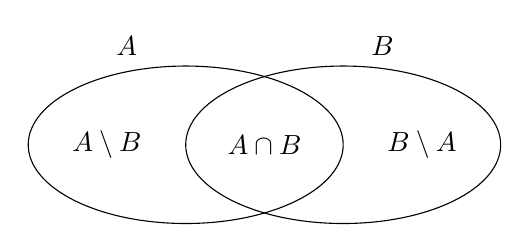
\begin{tikzpicture}[scale=0.5]
\draw (-3.5,1.5) ellipse (4 and 2);
\draw (0.5,1.5) ellipse (4 and 2);
\node at (-5.5,1.5) {$A\setminus B$};
\node at (-1.5,1.5) {$A\cap B$};
\node at (2.5,1.5) {$B\setminus A$};
\node at (-5,4) {$A$};
\node at (1.5,4) {$B$};
\end{tikzpicture}
\end{center}
By writing $A = (A\setminus B ) \cup (A\cap B)$ and $B = (B\setminus A ) \cup (A\cap B)$ and using the additivity and positivity of $\mu$, we have
\bi{rCl}
\mu(A)+\mu(B)& = &\mu((A\setminus B ) \cup (A\cap B))+\mu((B\setminus A ) \cup (A\cap B))\\
& = &\mu(A\setminus B ) + 2\mu(A\cap B)+\mu(B\setminus A )\\
& = &\mu(A\cup B ) + \mu(A\cap B)\\
& \geq & \mu(A\cup B ).
\ei
\item We now extend this to finite unions by induction. Let $\{A_n\}_{n\in\N}$ be a sequence in $\Sigma$ and suppose that
\bse
\mu\biggl(\bigcup_{\,i=0}^{n}A_i\biggr)\leq \sum_{i=0}^{n}\mu(A_i)
\ese
for some $n\in \N$. Then, by part (a), we have
\bi{rCl}
\mu\biggl(\bigcup_{\,i=0}^{\,n+1}A_i\biggr) & = & \mu\biggl(A_{n+1}\cup\bigcup_{i=0}^{n}A_i\biggr)\\
& \leq &\mu (A_{n+1})+\mu\biggl(\bigcup_{\,i=0}^{n}A_i\biggr)\\
& \leq &\mu (A_{n+1})+\sum_{i=0}^{n}\mu(A_i)\\
& = & \sum_{i=0}^{n+1}\mu(A_i).
\ei
Hence, by induction on $n$ with base case $n=1$ and noting that the case $n=0$ is trivial (it reduces to $\mu(A_0)=\mu(A_0)$), we have
\bse
\forall \, n \in \N : \ \mu\biggl(\bigcup_{\,i=0}^{n}A_i\biggr)\leq \sum_{i=0}^{n}\mu(A_i).
\ese
\item Let $\{A_n\}_{n\in\N}$ be a sequence in $\Sigma$. Define $B_n:=\bigcup_{i=0}^nA_n$. Then, $\{B_n\}_{n\in\N}$ is an increasing sequence in $\Sigma$. Hence, by continuity from above of $\mu$, we have
\bi{rCl}
\mu\biggl(\bigcup_{\,n=0}^{\infty}A_n\biggr) &=& \mu\biggl(\bigcup_{\,n=0}^{\infty}B_n\biggr)\\
& = & \lim_{n\to\infty}\mu(B_n)\\
& = & \lim_{n\to\infty}\mu\biggl(\bigcup_{\,i=0}^{n}A_i\biggr)\\
& \leq & \lim_{n\to\infty}\sum_{i=0}^n\mu(A_i)\\
& = & \sum_{i=0}^\infty\mu(A_i)
\ei
which is what we wanted. \qedhere
\een
\eq

\bd
Let $(M,\Sigma,\mu)$ be a measure space. The measure $\mu$ is said to be \emph{finite}\index{finite measure} if there exists a sequence $\{A_n\}_{n\in\N}$ in $\Sigma$ such that $\bigcup_{n=0}^{\infty}A_n=M$ and
\bse
\forall \, n \in \N : \ \mu(A_n)<\infty.
\ese
\ed

\be
The counting measure on $(\N,\mathscr{P}(\N))$ is finite. To see this, define $A_n:=\{n\}$. Then, clearly $\bigcup_{n=0}^{\infty}A_n=\N$ and $\mu(A_n)=|\{n\}|=1<\infty$ for all $n\in \N$.
\ee



\subsection[\texorpdfstring{Borel $\sigma$-algebras}{Borel \textsigma-algebras}]{Borel $\sigma$-algebras}

We have already remarked the parallel between topologies and $\sigma$-algebras. A further similarity stems from the fact that, just like for topologies, interesting $\sigma$-algebras are hardly ever given explicitly, except in some simple cases. In general, they are defined implicitly by some membership condition.

\bp
Let $M$ be a set and let $\{ \Sigma_i : i \in I\}$ be a collection of $\s$-algebras on $M$. Define the set
\bse
\Sigma :=\bigcap_{i\in I}\Sigma_i = \{ A \in \mathscr{P}(M) \mid A \in \Sigma_i, \forall \, i \in I \}.
\ese
Then, $\Sigma$ is a $\s$-algebra on $M$.
\ep
\bq
We simply check that $\Sigma$ satisfies the defining properties of a $\sigma$-algebra.
\ben[label=(\roman*)]
\item We have $M \in \Sigma_i$ for all $i \in I$ and hence $ M \in \Sigma$.  
\item Let $A \in \Sigma$. Then, $A \in \Sigma_i$ for all $i \in I$
and, since each $\Sigma_i$ is a $\s$-algebra, we also have $M\setminus A \in \Sigma_i$ for all $i\in I$. Hence, $M\setminus A \in \Sigma$.
\item Let $\{A_n\}_{n\in\N}$ be a sequence in $\Sigma$. Then, $\{A_n\}_{n\in\N}$ is a sequence in each $\Sigma_i$. Thus,
\bse
\forall \, i\in I : \ \bigcup_{n=0}^{\infty}{A_n} \in \Sigma_i.
\ese
Hence, we also have $\bigcup_{n=0}^{\infty}{A_n} \in \Sigma$. \qedhere
\een
\eq

\bd
Let $M$ be a set and let $\mathcal{E}\subseteq\mathscr{P}(M)$ be a collection of subsets of $M$. The $\sigma$-algebra \emph{generated} by $\mathcal{E}$, denoted $\sigma(\mathcal{E})$, is the smallest $\sigma$-algebra on $M$ containing all the sets in $\mathcal{E}$. That is,
\bse
A\in\sigma(\mathcal{E}) \quad \Leftrightarrow \quad  \text{for all $\sigma$-algebras }\Sigma \text{ on } M :\ \mathcal{E}\subseteq \Sigma \, \Rightarrow\, A\in \Sigma
\ese
or, by letting $\{\Sigma_i\mid i\in I\}$ be the collection of $\sigma$-algebras on $M$ such that $\mathcal{E}\subseteq \Sigma$,
\bse
\sigma(\mathcal{E}):=\bigcap_{i\in I}\Sigma_i.
\ese
\ed
The set $\mathcal{E}$ is called a \emph{generating set} for $\sigma(\mathcal{E})$. Observe that the second characterisation makes it manifest that $\sigma(\mathcal{E})$ is indeed a $\sigma$-algebra on $M$ by the previous proposition.

\bt
Let $(M,\Sigma)$ be a measurable space. Then, $\Sigma=\sigma(\mathcal{E})$ for some $\mathcal{E}\subseteq\mathscr{P}(M)$.
\et

%That is, every $\sigma$-algebra on $M$ is generated by some collection of subsets of $M$. 
This generating construction immediately allows us to link the notions of topology and $\sigma$-algebra on a set $M$ via the following definition.

\bd
Let $(M,\mathcal{O})$ be a topological space. The \emph{Borel $\sigma$-algebra}\index{Borel $\sigma$-algebra} on $(M,\mathcal{O})$ is $\sigma(\mathcal{O})$. 
\ed

Recall that a topology on $M$ is a collection $\mathcal{O}\subseteq\mathscr{P}(M)$ of subsets of $M$ which contains $\varnothing$ and $M$ and is closed under finite intersections and arbitrary (even uncountable) unions. The elements of the topology are called \emph{open sets}.
Of course, while there many choices of $\sigma$-algebra on $M$, if we already have a topology $\mathcal{O}$ on $M$, then the associated Borel $\sigma$-algebra is very convenient choice of $\sigma$-algebra since, as we will soon see, it induces a measurable structure which is ``compatible'' with the already given topological structure.

This is, in fact, the usual philosophy in mathematics: we always let the stronger structures induce the weaker ones, unless otherwise specified. For instance, once we have chosen an inner product on a space, we take the norm to be the induced norm, which induces a metric, which in turn induces a topology on that space, from which we now know how to obtain a canonical $\sigma$-algebra. 

We remark that, while the Borel $\sigma$-algebra on a topological space is generated by the open sets, in general, it contains much more that just the open sets.

\be
Recall that the standard topology on $\R$, denoted $\mathcal{O}_{\R}$, is defined by
\bse
A\in \mathcal{O}_{\R} \quad \Leftrightarrow \quad \forall \, a\in A : \exists \, \varepsilon > 0 : \forall \, r \in \R : \ |r-a|<\varepsilon \, \Rightarrow\,  r\in A.
\ese
In fact, the elements of $\mathcal{O}_{\R}$ are at most countable unions of open intervals in $\R$. Consider now the Borel $\sigma$-algebra on $(\R,\mathcal{O}_{\R})$. Let $a<b$. Then, for any $n\in \N$, the interval $(a-\tfrac{1}{n},b)$ is open. Hence, $\{(a-\tfrac{1}{n},b)\}_{n\in \N}$ is a sequence in $\sigma(\mathcal{O}_{\R})$. Since $\sigma$-algebras are closed under countable intersections, we have
\bse
\bigcap_{n=0}^{\infty}(a-\tfrac{1}{n},b) = [a,b) \in \sigma(\mathcal{O}_{\R}).
\ese
Hence, $\sigma(\mathcal{O}_{\R})$ contains, in addition to all open intervals, also all half-open intervals. It is not difficult to show that it contains all closed intervals as well. In particular, since singletons are closed, $\sigma(\mathcal{O}_{\R})$ also contains all countable subsets of $\R$. In fact, it is non-trivial\footnoteurl{https://en.wikipedia.org/wiki/Borel_set#Non-Borel_sets}{} to produce a subset of $\R$ which is not contained in $\sigma(\mathcal{O}_{\R})$.
\ee

\subsection[\texorpdfstring{Lebesgue measure on $\R^d$}{Lebesgue measure on R\textasciicircum d}]{Lebesgue measure on $\R^d$}

\bd
Let $(M,\Sigma,\mu)$ be a measure space. If $A\in\Sigma$ is such that $\mu(A)=0$, then $A$ is called a \emph{null set}\index{null set} or a \emph{set of measure zero}. 
\ed

The following definition is not needed for the construction of the Lebesgue measure. However, since it is closely connected with that of null set and will be used a lot in the future, we chose to present it here.

\bd
Let $(M,\Sigma,\mu)$ be a measure space and let $P$ be some property or statement. We say that $P$ holds \emph{almost everywhere}\index{almost everywhere} on $M$ if
\bse
\exists \, Z\in \Sigma : \ \mu(Z) = 0 \, \text{ and } \, \forall \, m\in M\setminus Z : \, P(m).
\ese
\ed
In other words, the property $P$ is said to hold almost everywhere on $M$ if it holds everywhere on $M$ except for a null subset of $M$.
\be
Let $(M,\Sigma,\mu)$ be a measure space and let $f,g\cl M\to N$ be maps. We say that $f$ and $g$ are \emph{almost everywhere equal}, and we write $f=_{\mathrm{a.e.}}g$, if there exists a null set $Z\in \Sigma$ such that
\bse
\forall \, m\in M\setminus Z : \ f(m)=g(m).
\ese
The case $f=g$ corresponds to $Z=\varnothing$.
\ee

\bd
A measure $\mu\cl \Sigma\to [0,\infty]$ is said to be \emph{complete} if every subset of every null set is measurable, i.e.\
\bse
\forall \, A\in \Sigma :\forall \, B\in\mathscr{P}(A) : \ \mu(A)=0 \,\Rightarrow \, B\in\Sigma.
\ese
\ed
Note that since for any $A,B\in\Sigma$, $B\subseteq A$ implies $\mu(B)\leq\mu(A)$, it follows that every subset of a null set, if measurable, must also be a null set.

\bd
Let $(M,\Sigma,\mu)$ be a measure space and let $(M,+,\cdot)$ be a vector space. The measure $\mu$ is said to be \emph{translation-invariant} if
\bse
\forall \, m\in M : \forall \, A\in \Sigma : \quad A+m\in\Sigma\ \text{ and }\ \mu(A+m)=\mu(A),
\ese
where $A+m := \{a+m\mid a\in A\}$.
\ed

\bt
Let $\mathcal{O}_{\R^d}$ be the standard topology on $\R^d$. There exists a unique complete, translation-invariant measure 
\bse
\lambda^d\cl\sigma(\mathcal{O}_{\R^d})\to[0,\infty]
\ese
such that for all $a_i,b_i\in\R$ with $1\leq i\leq d$ and $a_i<b_i$, we have
\bse
\lambda^d\bigl([a_1,b_1)\times\cdots\times[a_d,b_d)\bigr) = \prod_{i=1}^d(b_i-a_i).
\ese
\et

\bd
The measure $\lambda^d$ is called the \emph{Lebesgue measure} on $\R^d$.
\ed

The superscript $d$ in $\lambda^d$ may be suppressed if there is no risk of confusion. Note that the Lebesgue measure on $\R$, $\R^2$ and $\R^3$ coincides with the standard notions of length, area and volume, with the further insight that these are only defined for the elements of the respective Borel $\sigma$-algebras.

\bp
The Lebesgue measure on $\R$ is finite.
\ep
\bq
Consider the sequence $\{[a_n,a_n+1)\}_{n\in\N}$ where
\bse
a_n = %\tfrac{1}{4} (-1)^n (2 n-1 + (-1)^n )
\begin{cases}
-\tfrac{1}{2}n & \text{ if $n$ is even}\\
\tfrac{1}{2}(n+1) & \text{ if $n$ is odd}.
\end{cases}
\ese
That is, $\{a_n\}_{n\in\N}$ is the sequence $(0,1,-1,2,-2,3,-3,\ldots)$.\\


\begin{center}
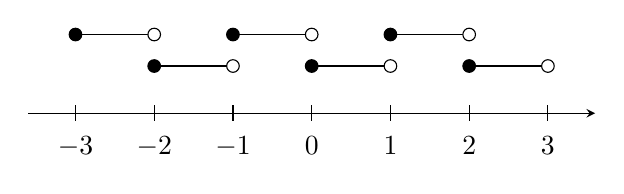
\begin{tikzpicture}
\foreach \i in {-3,-2,-1,0,1,2,3} {
\draw (\i,0.1)--(\i,-0.1) node[below=2pt] {$\i$};
};
\foreach \i in {-3,-1,1} {
 \foreach \j in {0,1} {
  \draw (\i+\j,1-0.4*\j)--(\i+\j+1,1-0.4*\j) ;
  \draw[fill] (\i+\j,1-0.4*\j) circle [radius=0.08] ;
  \draw[fill=white] (\i+\j+1,1-0.4*\j) circle [radius=0.08] ;
};};
\draw[->]  (-3.6,0)--(3.6,0);
\end{tikzpicture}
\end{center}
Clearly, we have $\bigcup_{n=0}^{\infty}[a_n,a_n+1) = \R$. Since, for all $n\in \N$, $[a_n,a_n+1)\in\sigma(\mathcal{O}_{\R})$ and $\lambda\bigl([a_n,a_n+1)\bigr) = 1<\infty$, the Lebesgue measure $\lambda$ is finite.
\eq

This can easily be generalised to show that $\lambda^d$ is finite for all $d\geq 1$.


\subsection{Measurable maps}

As we have remarked earlier, once we introduce a new structure, we should immediately think about the associated structure-preserving maps. In the case of measurable spaces, a measurable map is one that preserves the ``measurability'' structure.

\bd
Let $(M,\Sigma_M)$ and $(N,\Sigma_N)$ be measurable spaces. A map $f\cl M\to N$ is said to be \emph{measurable}\index{measurable map} if
\bse
\forall \, A\in \Sigma_N : \ \preim_f(A)\in \Sigma_M.
\ese
\ed

Note that this is exactly the definition of continuous map between topological spaces, with ``continuous'' replaced by ``measurable'' and topologies replaced by $\sigma$-algebras. 

\bl
Let $(M,\Sigma_M)$ and $(N,\Sigma_N)$ be measurable spaces. A map $f\cl M\to N$ is measurable if, and only if,
\bse
\forall \, A\in \mathcal{E} : \ \preim_f(A)\in \Sigma_M,
\ese
where $\mathcal{E}\subseteq\mathscr{P}(N)$ is a generating set of $\Sigma_N$.
\el

\bc
\label{cor:ContinuousMeasurable}
Let $(M,\mathcal{O}_M)$ and $(N,\mathcal{O}_N)$ be topological spaces. Any continuous map $M\to N$ is measurable with respect to the Borel $\sigma$-algebras on $M$ and $N$.
\ec

Recall that a map $\R\to\R$ is monotonic if it is either increasing or decreasing.

\bc
Any monotonic map $\R\to\R$ is measurable with respect to the Borel $\sigma$-algebra (with respect to $\mathcal{O}_{\R}$).
\ec

\bp
Let $(M,\Sigma_M)$, $(N,\Sigma_N)$ and $(P,\Sigma_P)$ be measurable spaces. If $f\cl M\to N$ and $g\cl N\to P$ are both measurable, the so is their composition $g \circ f\cl M\to P$.
\ep

\bq
Let $A\in \Sigma_P$. As $g$ is measurable, we have $\preim_g(A)\in\Sigma_N$. Then, since $f$ is measurable, it follows that
\bse
\preim_f(\preim_g(A)) = \preim_{g\circ f}(A) \in \Sigma_M.
\ese
Hence, $g\circ f$ is measurable.
\eq

\bp
\label{prp:MeasurablePointwiseLimit}
Let $(M,\Sigma_M)$ and $(N,\Sigma_N)$ be measurable spaces and let $\{f_n\}_{n\in\N}$ be a sequence of measurable maps from $M$ to $N$ whose pointwise limit is $f$. Then, $f$ is measurable.
\ep
Recall that $\{f_n\}_{n\in\N}$ converges pointwise to $f\cl M\to N$ if
\bse
\forall \, m\in M : \ \lim_{n\to \infty}f_n(m)=f(m).
\ese
This is in contrast with continuity, as pointwise convergence of a sequence of continuous maps is not a sufficient condition for the continuity of the pointwise limit. In the case of real or complex-valued maps, a sufficient condition is convergence with respect to the supremum norm. 

\subsection{Push-forward of a measure}

If we have a structure-preserving map $f$ between two instances $A$ and $B$ of some structure, and an object on $A$ (which depends in some way on the structure), we can often use $f$ to induce a similar object on $B$. This is generically called the push-forward of that object along the map $f$.

\bp
Let $(M,\Sigma_M,\mu)$ be a measure space, let $(N,\Sigma_N)$ be a measurable space and let $f\cl M\to N$ be a measurable map. Then, the map
\bi{rrCl}
f_*\mu\cl & \Sigma_N & \to & [0,\infty]\\
& A & \mapsto & \mu(\preim_f(A))
\ei
is a measure on $(N,\Sigma_N)$ called the \emph{push-forward}\index{push-forward of a measure} of $\mu$ along $f$.
\ep

That $f_*\mu$ is a measure follows easily from the fact that $\mu$ is a measure and basic properties of pre-images of maps, namely
\bi{rCl}
\preim_f(A\setminus B) & = & \preim_f(A)\setminus \preim_f(B)\\ \preim_f\biggl(\bigcup_{\,i\in I}A_i\biggr) & = & \bigcup_{i\in I}\preim_f(A_i).
\ei












\newpage

\section{Integration of measurable functions}

We will now focus on measurable functions $M\to \overline{\R}$ and define their integral on a subset of $M$ with respect to some measure on $M$, which is called the Lebesgue integral. Note that, even if $M\subseteq\R^d$, the Lebesgue integral of a function need not be with respect to the Lebesgue measure. 

The key application of this material is the definition of the Banach spaces of (classes of) Lebesgue integrable functions $L^p$. The case $p=2$ is especially important since $L^2$ is, in fact, a Hilbert space. It appears a lot in quantum mechanics where it is loosely referred to as the space of square-integrable functions.

\subsection{Characteristic and simple functions}

\bd
Let $M$ be a set and let $A\in\mathscr{P}(M)$. The \emph{characteristic function}\index{characteristic function} of $A$, denoted $\chi_A\cl M\to \R$, is defined by
\bse
\chi_A(m) = \begin{cases}1 & \text{if } m\in A\\ 0& \text{if } m\notin A.\end{cases}
\ese
\ed

\be
Below is the graph of $\chi_{(1,2]}\cl \R \to \R$.
\begin{center}
\begin{tikzpicture}[scale=1.2]
\draw[->] (0,-0.5)--(0,1.75);
\draw[->] (-0.5,0)--(3.5,0);
\foreach \i in {1,2,3}{
\draw (\i,0.08)--(\i,-0.08) node[below=2pt] {$\i$};
};
\draw (0.08,1) -- (-0.08,1) node[left] {$1$};
\draw (0,0) node[below left] {$0$};
\draw (1,1)--(2,1) node[right=3pt] {$\chi_{(1,2]}$};
\draw[dotted] (0,1)--(1,1)--(1,0);
\draw[dotted] (2,1)--(2,0);
\draw[fill=white] (1,1) circle [radius=0.08];
\draw[fill] (2,1) circle [radius=0.08];
\end{tikzpicture}
\end{center}
\ee

The following properties of characteristic functions are immediate.
\bp
\label{prp:characteristic}
Let $M$ be a set and let $A,B\in\mathscr{P}(M)$. Then
\ben[label=(\roman*)]
\item $\chi_{\varnothing}=0$
\item $\chi_{A\cup B} = \chi_A+\chi_B-\chi_{A\cap B}$
\item $\chi_{A\cap B} = \chi_A\chi_B$
\item $\chi_{M\setminus A} + \chi_A = 1$
\een
where the addition and multiplication are pointwise and the $0$ and $1$ in parts (i) and (iv) are the constant functions $M\to \R$ mapping every $m\in M$ to $0\in\R$ and $1\in\R$, respectively.
\ep

\bd
Let $M$ be a set. A function $s\cl M \to \R$ is \emph{simple}\index{simple function} if $s(M) = \{r_1,\ldots,r_n\}$ for some $n\in \N$. 
%Let $(M,\Sigma)$ be a measurable space. A measurable function $s\cl M \to \R$ is said to be \emph{simple}\index{simple function} if $s(M) = \{r_1,\ldots,r_n\}$ for some $n\in \N$. 
\ed
Equivalently, $s\cl M \to \R$ is simple if there exist $r_1,\ldots,r_n\in\R$ and $A_1,\ldots,A_n\in\mathscr{P}(M)$, for some $n\in \N$, such that
\bse
s = \sum_{i=1}^nr_i\chi_{A_i}.
\ese
So $s$ is simple if it is a linear combination of characteristic functions.
% Note that, since $s$ is assumed to be measurable, we have $\preim_s(\{r_i\})\in\Sigma$ for all $1\leq i\leq n$.

\be
Consider the simple function $s\cl \R \to \R$ given by $s:=\chi_{[1,3]}+2\chi_{[2,5]}$.
\begin{center}
\begin{tikzpicture}[scale=1.2]
\draw[->] (0,-0.5)--(0,3.75);
\draw[->] (-0.5,0)--(5.75,0);
\foreach \i in {1,2,3,4,5}{
\draw (\i,0.08)--(\i,-0.08) node[below=2pt] {$\i$};
};
\foreach \i in {1,2,3} {
\draw (0.08,\i) -- (-0.08,\i) node[left] {$\i$};
};
\draw (0,0) node[below left] {$0$};
\draw (1,1)--(2,1);
\draw (2,3)--(3,3);
\draw (3,2)--(5,2);
\draw[dotted] (0,1)--(1,1)--(1,0);
\draw[dotted] (0,3)--(2,3)--(2,0);
\draw[dotted] (0,2)--(3,2);
\draw[dotted] (3,3)--(3,0);
\draw[dotted] (5,2)--(5,0);
\draw[fill] (1,1) circle [radius=0.08];
\draw[fill=white] (2,1) circle [radius=0.08];
\draw[fill] (3,3) circle [radius=0.08];
\draw[fill] (2,3) circle [radius=0.08];
\draw[fill] (5,2) circle [radius=0.08];
\draw[fill=white] (3,2) circle [radius=0.08];
\end{tikzpicture}
\end{center}
By observing the graph, we see that we can re-write $s$ as
\bse
s = \chi_{[1,2)} + 3 \chi_{[2,3]} + 2 \chi_{(3,5]}.
\ese
\ee

\bd
A simple function is said to be in its \emph{standard form} if
\bse
s = \sum_{i=1}^nr_i\chi_{A_i},
\ese
where $A_i \cap A_j = \varnothing$ whenever $i\neq j$.
\ed

Any simple function can be written in standard form. It is clear that if $s$ is in its standard form, then $A_i = \preim_s(\{r_i\})$. 

\bp
Let $(M,\Sigma)$ be a measurable space and let $A,A_1,\ldots,A_n\in\mathscr{P}(M)$. Then
\ben[label=(\roman*)]
\item $\chi_A$ is measurable if, and only if, $A\in\Sigma$
\item if $s=\sum_{i=1}^n r_i \chi_{A_i}$ is a simple function in its standard form, then $s$ is measurable if, and only if, we have $A_i\in \Sigma$ for all $1\leq i\leq n$.
\een
\ep

\bq 
\ben[label=(\roman*)]
\item We have $\chi_A : M \to \R$ with possible values $\{0,1\}$. Equipping $\R$ with its Borel $\sigma$-algebra w.r.t. the standard topology, $\sigma(\cO_{\R})$, we have:
\ben
\item $(\Rightarrow)$ We have
\bse 
A = M\setminus \preim_{\chi_A}([0,1)),
\ese 
but $[0,1) \in \sigma(\cO_{\R})$ and so $\preim_{\chi_A}([0,1))\in \Sigma.$ Then by property (ii) of a $\sigma$-algebra $E\in\Sigma$.
\item $(\Leftarrow)$  Let $\alpha = [1,\infty)$, $\beta = (-\infty, 0)$ and $\gamma = [0,1]$. Clearly $\alpha,\beta,\gamma \in \sigma(\cO_{\R})$ and $\alpha\cup\beta\cup\gamma = \R$. Then 
\bi{rCl}
\preim_{\chi_A}(\alpha) & = & A, \\
\preim_{\chi_A}(\beta) & = & \varnothing, \\
\preim_{\chi_A}(\gamma) & = & M,
\ei 
all of which are measurable sets on $M$ and so $\chi_A$ is measurable.
\een 
\item First define $\widetilde{\chi}_{A_i} := r_i\chi_{A_i}$, which satisfies 
\bse
\widetilde{\chi}_{A_i}(m) = \begin{cases} r_i & \text{if } m\in A_i\\ 0& \text{if } m\notin A_i.\end{cases}
\ese
As $s$ is in its standard form we know $\widetilde{\chi}_{A_i} \cap \widetilde{\chi}_{A_j} = \varnothing$ for all $i\neq j$. Combining these two things, and defining $\alpha_i = [r_i,\infty)$, $\gamma_i = [0,r_i]$, the result follow from part (i).
\een 
\eq 

\subsection{Integration of non-negative measurable simple functions}

We begin with the definition of the integral of a non-negative, measurable, simple function.

\bd
Let $(M,\Sigma,\mu)$ be a measure space and let $s\cl M \to \R$ be a nowhere negative, measurable, simple function whose standard form is $s=\sum_{i=1}^n r_i \chi_{A_i}$. Then, we define
\bse
\int_M \! s \, \d \mu := \sum_{i=1}^nr_i\mu(A_i).
\ese
\ed

Note that the non-negativity condition is essential since $\mu$ takes values in $[0,\infty]$, hence we could have $\mu(A_i)=\infty$ for more that one $A_i$, and if the corresponding coefficients $r_i$ have opposite signs, then we would have $\int_Ms\,\d\mu=\infty-\infty$, which is not defined. For the same reason, we are considering $s\cl M\to [0,\infty)$ rather than $s\cl M\to [0,\infty]$.
\be
Consider the measure space $(\N,\mathscr{P}(\N),\mu)$, where $\mu$ is the counting measure, let $f\cl \N \to \R$ be non-negative and suppose that there exists $N\in\N$ such that $f(n)=0$ for all $n>N$. Then, we can write $f$ as
\bse
f=\sum_{n=0}^Nf(n)\chi_{\{n\}}.
\ese
That is, $f$ is a non-negative, measurable, simple function and therefore
\bse
\int_{\N}\! f \,\d \mu := \sum_{n=0}^Nf(n)\mu(\{n\}) = \sum_{n=0}^Nf(n).
\ese
Hence, the ``integral'' of $f$ over $\N$ with respect to the counting measure is just the sum.
\ee

The need for simple functions to be in their standard form, which was introduced to avoid any potential ambiguity in the definition of their integral, can be relaxed using the following lemma.

\bl
\label{lem:simplelinear}
Let $(M,\Sigma,\mu)$ be a measure space. Let $s$ and $t$ be non-negative, measurable, simple functions $M\to \R$ and let $c\in [0,\infty)$. Then
\bse
\int_M\!(cs+t)\,\d\mu = c\int_M\!s\,\d\mu+\int_M\!t\,\d\mu.
\ese
\el

\bp
\label{prp:MeasureIntegral}
Let $(M,\Sigma,\mu)$ be a measure space and let $s=\sum_{i=1}^n r_i \chi_{A_i}$ be a non-negative, measurable, simple function $M\to \R$ not necessarily in its standard form. Then
\bse
\int_M\!s\,\d\mu = \sum_{i=1}^nr_i\mu(A_i).
\ese
\ep

\bc
Let $(M,\Sigma,\mu)$ be a measure space. Let $s$ and $t$ be non-negative, measurable, simple functions $M\to \R$ such that $s\leq t$ (that is, $s(m)\leq t(m)$ for all $m\in M$). Then
\bse
\int_M\!s\,\d\mu \leq \int_M\!t\,\d\mu. 
\ese
\ec

\bl
Let $(M,\Sigma, \mu)$ be a measure space and let $s = \sum_{i=1}^n{r_i\chi_{A_i}}$ be a non-negative, measurable, simple function $M\to\R$. Define the map
\bi{rrCl}
\nu_s \cl & \Sigma & \to & [0,\infty]\\
& A & \mapsto &  \int_M \! s\chi_A \, \d \mu,
\ei
where $s\chi_A$ is the pointwise product of $s$ and $\chi_A$. Then, $\nu_s$ is a measure on $(M,\Sigma)$.
\el

\bq
First, note that we have
\bse
\int_M \! s\chi_A \, \d \mu = \int_M \biggl(\sum_{\,i=1}^nr_i\chi_{A_i}\chi_{A}\biggr) \d \mu = \int_M \biggl(\sum_{\,i=1}^nr_i\chi_{A_i\cap A}\biggr) \d \mu  =\sum_{i=1}^nr_i\mu({A_i\cap A)}.
\ese
We now check that $\nu$ satisfies the defining properties of a measure.
\ben[label=(\roman*)]
\item $\displaystyle\nu_s(\varnothing):= \int_M \! s\chi_{\varnothing} \, \d \mu = \sum_{i=1}^n{r_i\mu({A_i\cap \varnothing})} = \sum_{i=1}^n{r_i\mu(\varnothing)} = 0$
\item Let $\{B_j\}_{j\in\N}$ be a pairwise disjoint sequence in $\Sigma$. Then
\bi{rCl}
\nu_s \biggl( \bigcup_{\,j=0}^{\infty}B_j \biggr) &=& \int_M \! s\chi_{ \left( \bigcup_{j=0}^{\infty}B_j \right)} \, \d \mu \\
& = & \sum_{i=1}^n r_i  \mu \biggl( \bigcup_{\,j=0}^{\infty}(A_i \cap B_j )\biggr)\\
&=& \sum_{j=0}^{\infty}\sum_{i=1}^n r_i \mu (A_i \cap B_j )\\
&=& \sum_{j=0}^{\infty}\int_M \! s\chi_{B_j} \, \d \mu \\
&=& \sum_{j=0}^{\infty}\nu_s(B_j) .
\ei
\een
Thus, $\nu_s$ is a measure on $(M,\Sigma)$. \qedhere
\eq

\subsection{Integration of non-negative measurable functions}

As we are interested in measurable functions $M\to\overline{\R}$, we need to define a $\sigma$-algebra on $\overline{\R}$. We cannot use the Borel $\sigma$-algebra since we haven't even defined a topology on $\overline{\R}$. In fact, we can easily get a $\sigma$-algebra on $\overline{\R}$ as follows.

\bp
The set $\overline{\Sigma}:=\{A\in \mathscr{P}(\overline{\R})\mid A\cap \R \in \sigma(\mathcal{O}_{\R})\}$ is a $\sigma$-algebra on $\overline{\R}$.
\ep
In other words, we can simply ignore the infinities in a subset of $\overline{\R}$ and consider it to be measurable if $A\setminus\{-\infty,+\infty\}$ is in the Borel $\sigma$-algebra of $\R$. We will always consider $\overline{\R}$ to be equipped with this $\sigma$-algebra.

\bl
\label{lem:measurable}
Let $(M,\Sigma)$ be a measurable space and let $f,g\cl M\to \overline{\R}$ be measurable. Then, the following functions are measurable.
\ben[label=(\roman*)]
\item $cf+g$, for any $c\in \R$
\item $|f|$ and $f^2$
\item $fg$ (pointwise product) if $f$ and $g$ are nowhere infinite
\item $\max(f,g)$ (defined pointwise).
\een
\el


\bd
Let $(M,\Sigma,\mu)$ be a measure space and let $f\cl M\to\overline{\R}$ be a non-negative, measurable function. Denote by $S$ the set of all non-negative, measurable, simple functions $s\cl M \to \R$ such that $s\leq f$. Then, we define
\bse
\int_M\! f\, \d \mu := \sup_{s\in S} \int_M\! s\, \d \mu.
\ese
\ed

\br
It is often very convenient to introduce the notation
\bse
\int_M\!f(x)\,\mu(\d x) \equiv \int_M\! f\, \d \mu,
\ese
where $x$ is a dummy variable and could be replaced by any other symbol. The reason why this is a convenient notation is that, while some functions have standard symbols but cannot be easily represented by an algebraic expression (e.g. characteristic functions), others are easily expressed in terms of an algebraic formula but do not have a standard name. For instance, it is much easier to just write
\bse
\int_{\R}  x^2\,\mu(\d x)
\ese
than having to first denote the function $\R\to\R$, $x\mapsto x^2$ by a generic $f$ or, say, the more specific $\mathrm{sq}_{\R}$, and then write 
\bse
\int_\R\mathrm{sq}_{\R}\, \d \mu.
\ese
In computer programming, this is akin to defining \emph{anonymous functions}.
\er

\bd
Let $(M,\Sigma,\mu)$ be a measure space and let $f\cl M\to\overline{\R}$ be a non-negative, measurable function. For any $A\in \Sigma$ (that is, any measurable subset of $M$), we define
\bse
\int_A\! f\, \d \mu := \int_M\! f\chi_A\, \d \mu.
\ese
\ed
Note that the product $f\chi_A$ is measurable by part (iii) of \Cref{lem:measurable}.

\bl
\label{lem:intineq}
Let $(M,\Sigma,\mu)$ be a measure space, let $f,g\cl M\to\overline{\R}$ be non-negative, measurable functions such that $f\leq g$, and let $A,B\in \Sigma$ be such that $A\subseteq B$. Then
\ben[label=(\roman*)]
\item $\displaystyle \int_M\! f\, \d \mu \leq \int_M\! g\, \d \mu$
\item $\displaystyle \int_A\! f\, \d \mu \leq \int_B\! f\, \d \mu$.
\een
\el

\bq
\ben[label=(\roman*)]
\item Denote by $S_f$ and $S_g$ the sets of non-negative, measurable, simple functions that are less than or equal to $f$ and $g$, respectively. As $f\leq g$, we have $S_f\subseteq S_g$ and hence
\bse
\int_M\! f\, \d \mu :=  \sup_{s\in S_f}\, \int_M\! s\, \d \mu \leq \sup_{s\in S_g}\, \int_M\! s\, \d \mu =: \int_M\! g\, \d \mu.
\ese
\item Since $A\subseteq B$, for any $m\in M$ we have
\bse
f(m)\chi_A(m) \leq f(m)\chi_B(m).
\ese
In fact, we have equality whenever $m\in A$ or $m\in M\setminus B$, while for $m\in B\setminus A$ the left hand side is zero and the right-hand side is non-negative. Hence, $f\chi_A\leq f\chi_B$ and thus, by part (i), we have
\bse
\int_A\! f\, \d \mu := \int_M\! f\chi_A\, \d \mu \leq\int_M\! f\chi_B\, \d \mu =: \int_B\! f\, \d \mu \qedhere
\ese
\een
\eq

\bp[Markov inequality]
Let $(M,\Sigma,\mu)$ be a measure space and let $f\cl M\to\overline{\R}$ be a non-negative, measurable function. For any $z\in [0,\infty]$, we have
\bse
\int_M\! f\, \d \mu \geq z\, \mu(\preim_f([z,\infty])).
\ese
\ep

Equality is achieved whenever $z$ is an upper bound for $f$.

\begin{center}
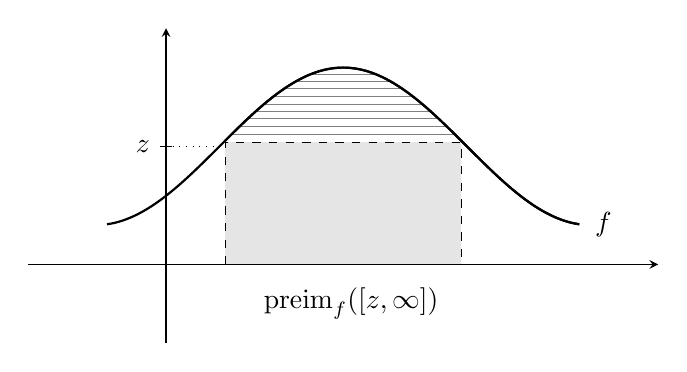
\begin{tikzpicture}
\foreach \i in {0.25,0.6,0.95,1.3,1.65,2.05,2.5,3,3.55} {
\draw[gray] (-0.5+0.3*\i,{1.5+cos deg (-0.5+0.3*\i-1)}) -- (2.5-0.3*\i,{1.5+cos deg (2.5-0.3*\i-1)}) ;
};
\fill[lightergray] (-0.5,0) rectangle (2.5,1.55);
\draw[dashed,thin] (-0.5,0)--(-0.5,1.55)--(2.5,1.55)--(2.5,0);
\draw (-1.17,1.5)--(-1.33,1.5) node[left] {$z$};
\draw (1.1,-0.5) node {$\preim_f([z,\infty])$};
\draw[dotted] (-1.25,1.5)--(-0.5,1.5);
\draw [thick,smooth,samples=100,variable=\x,domain=-2:4] plot(\x,{1.5+cos deg (\x-1)}) node[right=2pt] {$f$};
\draw [thick,smooth,samples=100,variable=\x,domain=-0.5:4] plot(\x,{1.5+cos deg (\x-1)});
\draw[->,thin] (-3,0)--(5,0);
\draw[->,thin] (-1.25,-1)--(-1.25,3);
\end{tikzpicture}
\end{center}

The following is the pivotal theorem of Lebesgue integration.

\bt[Monotone convergence theorem]
Let $(M,\Sigma,\mu)$ be a measure space and let $\{f_n\}_{n\in\N}$ be a sequence of non-negative, measurable functions $M\to\overline{\R}$ such that $f_{n+1}\geq f_n$ for all $n\in \N$. If there exists a function $f\cl M\to \overline{\R}$ such that
\bse
\forall \, m \in M : \ \lim_{n\to\infty}f_n(m) = f(m)
\ese
(i.e. $f$ is the pointwise limit of  $\{f_n\}_{n\in\N}$), then $f$ is measurable and
\bse
\lim_{n\to\infty}\int_M\! f_n \, \d \mu = \int_M\! f \, \d \mu.
\ese
\et

\br
Observe that this result is in stark contrast with what one may be used from Riemann integration, where pointwise converge of a sequence of integrable functions $\{f_n\}_{n\in\N}$ is \emph{not} a sufficient condition for the integral of the limit $f$ to be equal to the limit of the integrals of $f_n$ or, in fact, even for $f$ to be integrable. For these, we need stronger conditions on the sequence $\{f_n\}_{n\in\N}$, such as uniform converge.
\er

The definition of the integral as a supremum is clear and geometrically reasonable. However, it is in general very difficult to evaluate
the integral of any particular function using it. The monotone convergence theorem provides a much simpler way to evaluate the integral. One can show that, for any non-negative, measurable function $f$, there exists an increasing sequence $\{s_n\}_{n\in\N}$ of non-negative, measurable, simple functions (which can be explicitly constructed from $f$) whose pointwise limit is $f$, and hence we have
\bse
\int_M\! f \, \d \mu = \lim_{n\to\infty}\int_M\! s_n \, \d \mu,
\ese
where the right-hand side can usually be evaluated fairly easily.

\be
Consider the measure space $(\N,\mathscr{P}(\N),\mu)$, where $\mu$ is the counting measure, and let $f\cl \N \to \overline{\R}$ be non-negative. Note that the choice of $\sigma$-algebra $\mathscr{P}(\N)$ on $\N$ makes every function on $\N$ (to any measurable space) measurable. Define, for every $n\in \N$,  
\bse
s_n=\sum_{i=0}^nf(i)\chi_{\{i\}}.
\ese
Then, $\{s_n\}_{n\in\N}$ is an increasing sequence of non-negative, measurable, simple functions whose pointwise limit is $f$ and therefore, by the monotone convergence theorem,
\bse
\int_{\N}\! f \,\d \mu =\lim_{n\to\infty}\int_{\N}\! s_n \, \d \mu = \lim_{n\to\infty}\sum_{i=0}^nf(i)\mu(\{i\}) = \sum_{i=0}^{\infty}f(i).
\ese
If you ever wondered why series seem to share so many properties with integrals, the reason is that series are just integrals with respect to a discrete measure.
\ee

The monotone convergence theorem can be used to extend some of the properties of integrals of non-negative, measurable simple functions to non-negative, measurable functions which are not-necessarily simple.

\bl
Let $(M,\Sigma,\mu)$ be a measure space, let $f,g\cl M\to \overline{\R}$ be non-negative, measurable functions and let $c\in [0,\infty)$. Then
\ben[label=(\roman*)]
\item $\displaystyle \int_{M}\! (cf+g) \,\d \mu = c\int_{M}\! f \,\d \mu +\int_{M}\! g \,\d \mu $
\item the map $\nu_f\cl \Sigma\to [0,\infty]$ defined by $\displaystyle \nu_f(A):=\int_A\, f\, \d \mu$ is a measure on $(M,\Sigma)$
\item for any $A\in\Sigma$, we have $\displaystyle \int_{M}\!f \,\d \mu =  \int_{A}\!f \,\d \mu+ \int_{M\setminus A}\!f \,\d \mu$.
\een
\el

\bq
\ben[label=(\roman*)]
\item Let $\{s_n\}_{n\in\N}$ and $\{t_n\}_{n\in\N}$ be increasing sequences of non-negative, measurable, simple functions whose pointwise limits are $f$ and $g$, respectively. Then, it is easy to see that $\{cs_n+t_n\}_{n\in\N}$ is an increasing sequence of non-negative, measurable, simple functions whose pointwise limit is $cf+g$. Hence, by \Cref{lem:simplelinear} and the monotone converge theorem
\bi{rCl}
\int_M\! (cf+g) \,\d \mu & = &  \lim_{n\to\infty}\int_M\! (cs_n+t_n) \, \d \mu\\
& = &  \lim_{n\to\infty}\biggl(c\int_M\! s_n \, \d \mu+\int_M\! t_n \, \d \mu\biggr)\\
& = &  c\lim_{n\to\infty}\int_M\! s_n \, \d \mu+\lim_{n\to\infty}\int_M\! t_n \, \d \mu\\
& = &  c\int_{M}\! f \,\d \mu +\int_{M}\! g \,\d \mu.
\ei
\item To check that $\nu_f$ is a measure on $(M,\Sigma)$, first note that we have
\bse
\nu_f(\varnothing) = \int_{\varnothing}\! f\, \d \mu :=\int_{M}\! f\chi_{\varnothing}\, \d \mu = 0.
\ese
Let $\{A_i\}_{i\in\N}$ be a pairwise disjoint sequence in $\Sigma$. Define, for any $n\in \N$,
\bse
f_n:=f\chi_{\left(\bigcup_{i=0}^nA_i\right)}.
\ese
Since, for all $n\in \N$, we have $\bigcup_{i=0}^{n}A_i\subseteq\bigcup_{i=0}^{n+1}A_i$ and $f$ is non-negative, $\{f_n\}_{n\in\N}$ is an increasing sequence of non-negative, measurable, simple functions whose pointwise limits is $f\chi_{\left(\bigcup_{i=0}^{\infty}A_i\right)}$. Hence, by recalling \Cref{prp:characteristic}, we have
\bi{rCl}
\nu_f\biggl(\bigcup_{\,i=0}^{\infty}A_i\biggr) & := & \int_{\,\bigcup_{i=0}^{\infty}A_i}\! f \, \d \mu\\
& = & \int_{M} \!f\chi_{\left(\bigcup_{i=0}^{\infty}A_i\right)} \, \d \mu\\
& = & \lim_{n\to\infty}\int_{M} \!f\chi_{\left(\bigcup_{i=0}^{n}A_i\right)} \, \d \mu\\
& = & \lim_{n\to\infty}\int_{M} \biggl(f\sum_{i=0}^{n}\chi_{A_i}\biggr) \, \d \mu\\
& = & \lim_{n\to\infty}\biggl(\sum_{\,i=0}^{n}\int_{M}\! f\chi_{A_i}\, \d \mu\biggr) \\
& = & \sum_{i=0}^{\infty}\nu_f(A_i) .
\ei
\item Note that $A\cap (M\setminus A)=\varnothing$. Hence, by using the fact that $\nu_f$ from part (ii) is a measure on $(M,\Sigma)$, we have
\bse
\int_M\! f \, \d \mu  =  \nu_f(M) =  \nu_f(A)+\nu_f(M\setminus A) =  \int_A\! f\, \d \mu + \int_{M\setminus A}\! f\, \d \mu. \qedhere
\ese
\een
\eq

Part (i) of the previous lemma and the monotone convergence theorem also imply that, for any sequence $\{f_n\}_{n\in\N}$ of non-negative, measurable functions, we have
\bse
\int_M \biggl(\sum_{\,n=0}^{\infty}f_n \biggr) \d \mu = 
\sum_{n=0}^{\infty} \int_M \! f_n \, \d \mu.
\ese
Again, note that this result does \emph{not} hold for the Riemann integral unless stronger conditions are places on the sequence $\{f_n\}_{n\in\N}$.

Finally, we have a simple but crucial result for Lebesgue integration.

\bt
\label{thm:aezero}
Let $(M,\Sigma,\mu)$ be a measure space and let $f\cl M\to\overline{\R}$ be a non-negative, measurable function. Then
\bse
\int_M\! f\, \d \mu = 0 \quad \Leftrightarrow \quad f=_{\mathrm{a.e.}} 0.
\ese
\et

\bq
\begin{itemize}
\item[$(\Rightarrow)$] Suppose that $\int_Mf\,\d\mu=0$. Define $A_n:=\{m\in M \mid f(m)>\tfrac{1}{n+1}\}$ and let
\bse
s_n := \tfrac{1}{n+1}\chi_{A_n} .
\ese
By definition of $A_n$, we clearly have $s_n\leq f$ for all $n\in\N$. Hence,
\bse
0\leq \int_M\!s_n\,\d\mu\leq\int_M\!f\,\d\mu=0
\ese
and thus, $\int_Ms_n\,\d\mu=0$ for all $n\in\N$. Since by definition
\bse
\int_M\!s_n\,\d\mu = \tfrac{1}{n+1}\mu(A_n),
\ese
we must also have $\mu(A_n)=0$ for all $n\in\N$. Let $A:=\{m\in M \mid f(m)\neq 0\}$. Then, as $f$ is non-negative, we have
\bse
A = \bigcup_{n=0}^{\infty}A_n=\bigcup_{n=0}^{\infty}\{m\in M \mid f(m)>\tfrac{1}{n+1}\}
\ese
and, since $A_n\subseteq A_{n+1}$ for all $n\in\N$, we have
\bse
\mu(A)=\mu\biggl(\bigcup_{\,n=0}^{\infty}A_n\biggr)=\lim_{n\to\infty}\mu(A_n) = 0.
\ese
Thus, $f$ is zero except on the null set $A$. That is, $f=_{\mathrm{a.e.}}0$. 

\item[$(\Leftarrow)$] Suppose that $f=_{\mathrm{a.e.}}0$. Let $S$ be the set of non-negative, measurable, simple functions $s$ such that $s\leq f$. As $f=_{\mathrm{a.e.}}0$, we have $s=_{\mathrm{a.e.}}0$ for all $s\in S$. Thus, if
\bse
s=\sum_{i=1}^nr_i\chi_{A_i},
\ese
we must have either $r_i=0$ or $\mu(A_i)=0$ for all $1\leq i\leq n$. Hence, for all $s\in S$,
\bse
\int_M\! s \, \d \mu := \sum_{i=1}^nr_i\mu(A_i) =0.
\ese
Therefore, we have
\bse
\int_M\! f \, \d \mu := \sup_{s\in S}\int_M\! s \, \d \mu  = 0.\qedhere
\ese
\end{itemize}
\eq

This means that, for the purposes of Lebesgue integration, null sets can be neglected as they do not change the value of an integral. The following are some examples of this.

\bc
Let $(M,\Sigma,\mu)$ be a measure space, let $A\in\Sigma$ and let $f,g\cl M\to\overline{\R}$ be non-negative, measurable functions. 
\ben[label=(\roman*)]
\item If $\mu(A)=0$, then $\displaystyle\int_A\! f \, \d \mu = 0$
\item If $f=_{\mathrm{a.e.}}g$, then $\displaystyle\int_M\! f \, \d \mu = \int_M\! g \, \d \mu$
\item If $f\leq_{\mathrm{a.e.}}g$, then $\displaystyle\int_M\! f \, \d \mu \leq \int_M\! g \, \d \mu$.
\een
\ec

\bq
\ben[label=(\roman*)]
\item Clearly, $f\chi_A =_{\mathrm{a.e.}}0$ and hence
\bse
\int_A\! f \, \d \mu =\int_M\! f\chi_A  \, \d \mu = 0.
\ese
\item As $f=_{\mathrm{a.e.}}g$, we have $f-g=_{\mathrm{a.e.}}0$ and thus
\bse
0 = \int_M\! (f-g) \, \d \mu =\int_M\! f \, \d \mu-\int_M\! g \, \d \mu.
\ese
\item Let $B:=\{m\in M\mid f(m)>g(m)\}$. As $f\leq_{\mathrm{a.e.}}g$, we have $\mu(B)=0$ and $f\leq g$ on $M\setminus B$. Thus
\bi{C}
\int_M\! f \, \d \mu =\int_B\! f \, \d \mu+\int_{M\setminus B}\! f \, \d \mu
 \leq  \int_{M\setminus B}\! g \, \d \mu \leq \int_M\! g \, \d \mu
\ei
where we used part (i) and \Cref{lem:intineq}. \qedhere
\een
\eq

\be
Consider $(\R,\sigma(\mathcal{O}_{\R}),\lambda)$ and let $f\cl \R \to \R$ be the \emph{Dirichlet function}
\bse
f(r) := \begin{cases}
1 & \text{if } r\in \Q\\
0 & \text{if } r\in \R\setminus \Q.
\end{cases}
\ese
The Dirichlet function is the usual example of a function which is \emph{not} Riemann integrable (on any real interval). We will now show that we can easily assign a numerical value to its integral on any measurable subset of $\R$. First, note that a set $A\in\sigma(\mathcal{O}_{\R})$ is null with respect to the Lebesgue measure if, and only if, 
\bse
\forall \, \varepsilon >0 : \exists \, \{I_n\}_{n\in\N} : \quad A\subset \bigcup_{n=0}^{\infty}I_n \ \text{ and } \ \sum_{n=0}^{\infty}\lambda(I_n)<\varepsilon
\ese
where $\{I_n\}_{n\in\N}$ is a sequence of real intervals. From this, it immediately follows that any countable subset of $\R$ has zero Lebesgue measure. Thus, $\lambda(\Q)=0$ and hence, $f=_{\mathrm{a.e.}}0$. Therefore, by the previous lemmas, we have
\bse
\int_A\! f \, \d \lambda = 0
\ese
for any measurable subset $A$ of $\R$. 
\ee

\subsection{Lebesgue integrable functions}

Since the difference $\infty-\infty$ is not defined, we cannot integrate all measurable functions. There is, however, a very small extra condition (beyond measurability) that determines the class of functions to which we can extend our previous definition.

\bd
Let $(M,\Sigma,\mu)$ be a measure space and let $f\cl M\to\overline{\R}$. The function $f$ is said to be \emph{(Lebesgue) integrable}\index{integrable function} if it is measurable and
\bse
\int_{M}\!|f|\,\d \mu < \infty.
\ese
We denote the set of all integrable functions $M\to\overline{\R}$ by $\mathscr{L}^1_{\R}(M,\Sigma,\mu)$, or simply $\mathscr{L}^1(M)$ if there is no risk of confusion.
\ed

For any $f\cl M\to \overline{\R}$, we define $f^+:=\max(f,0)$ and $f^-:=\max(-f,0)$, which are measurable whenever $f$ is measurable by part (iv) of \Cref{lem:measurable}.

\bse
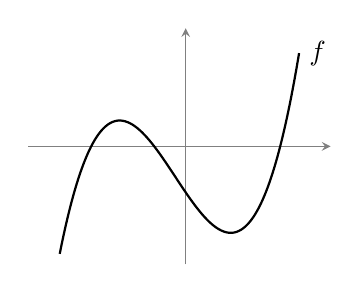
\begin{tikzpicture}[xscale=0.4,yscale=0.5]
\draw[->,thin,gray] (-5,0)--(4.6,0);
\draw[->,thin,gray] (0,-3)--(0,3);
\draw [thick,smooth,samples=100,variable=\x,domain=-4:3.6] plot(\x,{(\x+1)*(\x-3)*(\x+3)*0.13}) node[right] {$f$};
\end{tikzpicture}
\qquad\
\begin{tikzpicture}[xscale=0.4,yscale=0.5]
\draw[->,thin,gray] (-5,0)--(4.6,0);
\draw[->,thin,gray] (0,-3)--(0,3);
\draw [thick,smooth,samples=100,variable=\x,domain=-3:-1] plot(\x,{(\x+1)*(\x-3)*(\x+3)*0.13});
\draw [thick,smooth,samples=100,variable=\x,domain=3:3.6] plot(\x,{(\x+1)*(\x-3)*(\x+3)*0.13}) node[right] {$f^+$};
\draw [thick] (-4,0)--(-3,0);
\draw [thick] (-1,0)--(3,0);
\end{tikzpicture}
\qquad\
\begin{tikzpicture}[xscale=0.4,yscale=0.5]
\draw[->,thin,gray] (-5,0)--(4.6,0);
\draw[->,thin,gray] (0,-3)--(0,3);
\draw [thick,smooth,samples=100,variable=\x,domain=-4:-3] plot(\x,{-(\x+1)*(\x-3)*(\x+3)*0.13});
\draw [thick,smooth,samples=100,variable=\x,domain=-1:3] plot(\x,{-(\x+1)*(\x-3)*(\x+3)*0.13}) node[above=20pt] {$\ f^-$};
\draw [thick] (-3,0)--(-1,0);
\draw [thick] (3,0)--(3.7,0);
\end{tikzpicture}
\ese
Observe that $f=f^+-f^-$ and $|f|=f^++f^-$. Clearly, we have $f^+\leq|f|$ and $f^-\leq |f|$, and hence


\bse
\int_{M}\!|f|\,\d \mu < \infty\quad \Leftrightarrow \quad \int_{M}\!f^+\,\d \mu < \infty\ \text{ and } \int_{M}\!f^-\,\d \mu < \infty.
\ese


\bd
Let $(M,\Sigma,\mu)$ be a measure space and let $f\cl M\to\overline{\R}$ be integrable. Then, the \emph{(Lebesgue) integral}\index{Lebesgue integral} of $f$ over $M$ with respect to $\mu$ is
\bse
\int_{M}\!f\,\d \mu := \int_{M}\!f^+\,\d \mu -\int_{M}\!f^-\,\d \mu .
\ese
\ed

It should be clear that the role of the integrability condition $\int_M |f|\, \d \mu<\infty$ is to prevent the integral of $f$ from being $\infty-\infty$, which is not defined.

In quantum mechanics, we usually deal with complex functions. The extension to the complex case of the integration theory presented thus far is straightforward.

\bd
Let $(M,\Sigma,\mu)$ be a measure space. A complex function $f\cl M\to\C$ is said to be \emph{integrable} if the real functions $\Re(f)$ and $\Im(f)$ are measurable and
\bse
\int_{M}\!|f|\,\d \mu < \infty,
\ese
where $|f|$ denotes the complex modulus, i.e.\ $|f|^2=\Re(f)^2+\Im(f)^2$. We denote the set of all integrable complex functions by $\mathscr{L}^1_{\C}(M,\Sigma,\mu)$, or simply $\mathscr{L}^1(M)$ if there is no risk of confusion.
\ed

\bd
Let $(M,\Sigma,\mu)$ be a measure space and let $f\cl M\to\C$ be integrable. We define
\bse
\int_{M}\!f\,\d \mu := \int_{M}\!\Re(f)\,\d \mu +\mathrm{i}\int_{M}\!\Im(f)\,\d \mu .
\ese
\ed







The following lemma gives the properties expected of sums and scalar multiples of integrals. Note, however, that before we show that, say, the integral of a sum is the sum of the integrals, it is necessary to first show that the sum of two functions in $\mathscr{L}^1(M)$ is again in $\mathscr{L}^1(M)$.

\pagebreak

\bl
\label{lem:l1vs}
Let $(M,\Sigma,\mu)$ be a measure space, let $f,g \in \mathscr{L}^1(M)$ and let $c \in \R$. Then
\ben[label=(\roman*)]
\item $|f| \in \mathscr{L}^1(M)$ and $ \displaystyle \biggl| \int_M \! f \, \d \mu \biggr| \leq \int_M \! | f| \, \d \mu $
\item $c f \in \mathscr{L}^1(M)$ and $ \displaystyle \int_M \! cf \, \d \mu = c \int_M \!  f \, \d \mu$
\item $f+g \in \mathscr{L}^1(M)$ and $ \displaystyle \int_M \! (f+g) \, \d \mu = \int_M \!  f \, \d \mu +  \int_M \!  g \, \d \mu$
\item $\mathscr{L}^1(M)$ is a vector space.
\een
\el

\bq
\ben[label=(\roman*)]
\item As $\bigl| |f| \bigr|=|f|$, we have $|f| \in \mathscr{L}^1(M)$. Then, by the triangle inequality,
\bi{rCl}
\left|  \int_M \! f \, \d \mu \right| &=& \left|  \int_M \! f^+ \, \d \mu -   \int_M \! f^- \, \d \mu \right|\\
& \leq & \left|  \int_M \! f^+ \, \d \mu  \right| + \left| \int_M \! f^- \, \d \mu \right|\\
&=&  \int_M \! f^+ \, \d \mu + \int_M \! f^- \, \d \mu \\
&=&  \int_M \! (f^+ + f^-)\, \d \mu  \\
&=& \int_M \!  |f| \, \d \mu.
\ei 
\item We have
\bse
\int_M \!  |c f| \, \d \mu = \int_M \!  |c||f| \, \d \mu = |c|\int_M \!  | f| \, \d \mu< \infty
\ese
and hence, we have $c f \in \mathscr{L}^1(M)$.

\noindent Suppose $c \geq 0$. Then, $(c f)^+ = cf^+$ and $(c f)^- = c f^-$ and thus
\bi{rCl}
 \int_M \!c f \, \d \mu  &=& \int_M \! (c f)^+ \, \d \mu -   \int_M \! (c f)^- \, \d \mu\\
&=& \int_M \! c f^+ \, \d \mu -   \int_M \! c f^- \, \d \mu\\
&=&  c\int_M \! f^+ \, \d \mu -c \int_M \! f^- \, \d \mu \\
&=&  c\int_M \! (f^+ -f^-)\, \d \mu  \\
&=& c\int_M \!  f \, \d \mu
\ei 
Now suppose $c = -1$. Then, $(- f)^+ = f^-$ and $(- f)^- = f^+$. Thus
\bi{rCl}
 \int_M \! (-f) \, \d \mu  &=& \int_M \! (- f)^+ \, \d \mu -   \int_M \! (- f)^- \, \d \mu\\
&=& \int_M \! f^- \, \d \mu -   \int_M \!  f^+ \, \d \mu\\
&=& -\biggl( \int_M \! f^+ \, \d \mu - \int_M \! f^- \, \d \mu \biggr) \\
&=&  -\int_M \! (f^+ -f^-)\, \d \mu  \\
&=& -\int_M \!  f \, \d \mu.
\ei 
The case $c < 0$ follows by writing $c = (-1)(-c) $ and applying the above results.
\item By the triangle inequality, we have $|f+g| \leq | f| +| g|$ and thus
\bse
\int_M \!  |f+g| \, \d \mu \leq \int_M \!  |f| \, \d \mu + \int_M \!  |g| \, \d \mu < \infty.
\ese
Hence, $f+g \in \mathscr{L}^1(M)$. Moreover, we have
\bse
f+g = f^+ -f^- + g^+ -g^- = (f^++g^+)-(f^-+g^-),
\ese
where $f^++g^+$ and $f^-+g^-$ are non-negative and measurable. Note that, while $(f+g)^+\neq f^++g^+$ and $(f+g)^-\neq f^-+g^-$, one can show that $f^++g^+$ and $f^-+g^-$ give an equivalent splitting of $f+g$ to define its integral.
%with
% \bse
% \int_M \! (f^-+g^-)\, \d \mu = \int_M \! f^- \, \d \mu + \int_M \! g^- \, \d \mu < \infty .
% \ese
Therefore
\bi{rCl}
 \int_M \! (f+g) \, \d \mu  &=& \int_M \!  (f^++g^+) \, \d \mu - \int_M \! (f^-+g^-) \, \d \mu\\
 &=& \int_M \!  f^+ \, \d \mu + \int_M \!  g^+ \, \d \mu - \int_M \! f^- \, \d \mu - \int_M \! g^- \, \d \mu   \\
&=&  \int_M \! (f^+ -f^-)\, \d \mu  + \int_M \! (g^+ -g^-)\, \d \mu\\
&=& \int_M \!  f \, \d \mu + \int_M \!  g \, \d \mu.
\ei 
\item The set of all functions from $M$ to $\overline{\R}$ is a vector space. By parts (ii) and (iii), we have that $\mathscr{L}^1(M)$ is a vector subspace of this vector space and hence, a vector space in its own right. \qedhere
\een
\eq

Some properties of the integrals of non-negative, measurable functions easily carry over to general integrable functions.

\bl
Let $(M,\Sigma,\mu)$ be a measure space and let $f,g \in \mathscr{L}^1(M)$. 
\ben[label=(\roman*)]
\item If $f=_{\mathrm{a.e.}}g$, then $\displaystyle \int_M\! f \, \d \mu = \int_M\! g \, \d \mu$
\item If $f\leq_{\mathrm{a.e.}}g$, then $\displaystyle \int_M\! f \, \d \mu \leq \int_M\! g \, \d \mu$.
\een
\el

Just as the monotone convergence theorem was very important for integrals of non-negative, measurable functions, there is a similar theorem that is important for integrals of functions in $\mathscr{L}^1(X)$.

\bt[Dominated convergence theorem]
Let $(M,\Sigma,\mu)$ be a measure space and let $\{f_n\}_{n\in\N}$ be a sequence of measurable functions which converges almost everywhere to a measurable function $f$. If there exists $g \in \mathscr{L}^1(M)$ such that $|f_n| \leq_{\mathrm{a.e.}} g$ for all $n \in \N$, then
\ben[label=(\roman*)]
\item $f \in \mathscr{L}^1(M)$ and $f_n \in \mathscr{L}^1(M)$ for all $n \in \N$
\item $\displaystyle \lim_{n \to \infty} \int_M \!  |f_n-f| \, \d \mu =0$
\item $\displaystyle \lim_{n \to \infty} \int_M \!  f_n \, \d \mu = \int_M \!  f \, \d \mu$.
\een
\et

\br
By ``$\{f_n\}_{n\in\N}$ converges almost everywhere to $f$'' we mean, of course, that there exists a null set $A\in\Sigma$ such that
\bse
\forall \, m \in M\setminus A : \ \lim_{n\to\infty}f_n(m)=f(m).
\ese
\er


\subsection[\texorpdfstring{The function spaces $L^p(M,\Sigma,\mu)$}{The function spaces L\textasciicircum p(M,\textSigma,\textmu)}]{The function spaces $L^p(M,\Sigma,\mu)$}


While in quantum mechanics we need the theory of $L^p$ spaces only for $p=2$, it is worthwhile to develop the theory in more generality, by considering $L^p$ for all $1\leq p\leq \infty$.

\bd
Let $(M,\Sigma,\mu)$ be a measure space and let $p\in [1,\infty)$. We define
\bse
\mathscr{L}^p_{\R}(M,\Sigma,\mu) := \biggl\{f\cl M \to \overline{\R}\ \Big| \ f \text{ is measurable and } \int_M\!|f|^p\,\d \mu < \infty\biggr\}
\ese
and, similarly,
\bse
\mathscr{L}^p_{\C}(M,\Sigma,\mu) := \biggl\{f\cl M \to \C\ \Big| \ \Re(f) \text{ and } \Im(f) \text{ are measurable and } \int_M\!|f|^p\,\d \mu < \infty\biggr\}.
\ese
Whenever there is no risk of confusion, we lighten the notation to just $\mathscr{L}^p$.
\ed


\bd
Let $(M,\Sigma,\mu)$ be a measure space and let $f\cl M \to \overline{\R}$. The \emph{essential supremum}\index{essential supremum} of $f$ is defined as
\bse
\esup%_M
f := \inf\{c\in\overline{\R}\mid f \leq_{\mathrm{a.e.}}c\}.
\ese
Then, $f$ is said to be \emph{almost everywhere bounded (from above)} if $\esup f < \infty$. 
\ed

Alternatively, $f\cl M \to \overline{\R}$ is almost everywhere bounded if there exists a null set $A\in \Sigma$ such that $f$ restricted to $M\setminus A$ is bounded.

\bd
Let $(M,\Sigma,\mu)$ be a measure space. We define
\bse
\mathscr{L}^{\infty}_{\R}(M,\Sigma,\mu) := \biggl\{f\cl M \to \overline{\R}\ \Big| \ f \text{ is measurable and } \esup |f| < \infty\biggr\}
\ese
and, similarly,
\bse
\mathscr{L}^{\infty}_{\C}(M,\Sigma,\mu) := \biggl\{f\cl M \to \C\ \Big| \ \Re(f) \text{ and } \Im(f) \text{ are measurable and } \esup |f| < \infty\biggr\}.
\ese
Whenever there is no risk of confusion, we lighten the notation to just $\mathscr{L}^p$, for $p\in[1,\infty]$.
\ed

All the $\mathscr{L}^p$ spaces become vector spaces once equipped with pointwise addition and multiplication. Let us show this is detail for $\mathscr{L}_{\C}^2$.

\bp
Let $(M,\Sigma,\mu)$ be a measure space. Then, $\mathscr{L}_{\C}^2$ is a complex vector space.
\ep

\bq
The set of all functions $M\to\C$, often denoted $M^{\C}$, is a vector space under pointwise addition and multiplication. Hence, it suffices to show that $\mathscr{L}_{\C}^2$ is a subspace of $M^{\C}$.
\ben[label=(\roman*)]
\item Let $f \in \mathscr{L}_{\C}^2$ and $z\in \C$. As $|z|\in \R$, we have:
\bse
\int_M \!  |z f|^2 \, \d \mu = |z|^2 \int_M \!  |f|^2 \, \d \mu < \infty
\ese
and hence, $z f \in \mathscr{L}_{\C}^2$.
\item Let $f,g \in \mathscr{L}_{\C}^2$. Note that
\bi{rCl}
|f+g|^2  &=& (f+g)\overline{(f+g)}\\
&=& (f+g)(\overline{f}+\overline{g})\\
&=&  f\overline{f}+f\overline{g}+g\overline{f}+g\overline{g} \\
&=&   |f|^2 +f\overline{g}+g\overline{f}+ |g|^2.
\ei 
Moreover, as
\bse
0 \leq |f-g|^2 = |f|^2 -f\overline{g}-g\overline{f}+ |g|^2 ,
\ese
we have $f\overline{g}+g\overline{f} \leq |f|^2+ |g|^2$, and thus
\bse
|f+g|^2 \leq 2 |f|^2+ 2|g|^2.
\ese
Therefore
\bse
\int_M \!  |f+g|^2 \, \d \mu \leq 2\int_M \!  |f|^2 \, \d \mu + 2\int_M \!  |g|^2 \, \d \mu  < \infty ,
\ese
and hence $f+g \in \mathscr{L}_{\C}^2$.\qedhere
\een
\eq

Ideally, we would like to turn all these $\mathscr{L}^p$ space into Banach spaces. Let us begin by equipping them with a weaker piece of extra structure.

\bp
\label{prp:NormLp}
Let $(M,\Sigma,\mu)$ be a measure space and let $p\in[0,\infty]$. Then, the maps $\|\cdot\|_p\cl \mathscr{L}^p\to\R$ defined by
\bse
\|f\|_p:=
\begin{cases}
\biggl(\displaystyle\int_M\! |f|^p\,\d \mu\biggr)^{\negmedspace\frac{1}{p}} & \text{ for } 1\leq p<\infty\\
\esup |f| & \text{ for }p=\infty
\end{cases}
\ese
are semi-norms on $\mathscr{L}^p$. That is, for all $z\in \C$ and $f,g\in\mathscr{L}^p$,
\ben[label=(\roman*)]
\item $\|f\|_p\geq 0$
\item $\|z f\|_p = |z|\|f\|_p$
\item $\|f+g\|_p\leq\|f\|_p+\|g\|_p$.
\een
\ep
In other words, the notion of semi-norm is a generalisation of that of norm obtained by relaxing the definiteness condition. If the measure space $(M,\Sigma,\mu)$ is such that the empty set is the only null set, then $\|\cdot\|_p$ is automatically definite and hence, a norm.

\be
Consider $(\N,\mathscr{P}(\N),\mu)$, where $\mu$ is the counting measure. Then, as $\mu(A)$ is the cardinality of $A$, the only null set is the empty set. Thus, recalling that functions on $\N$ are just sequences, the maps
\bse
\|\{a_n\}_{n\in\N}\|_p = 
\begin{cases}
\biggl(\displaystyle\sum_{\,n=0}^{\infty} |a_n|^p\biggr)^{\negmedspace\frac{1}{p}} & \text{ for } 1\leq p<\infty\\
\sup \{|a_n| \mid n\in \N\} & \text{ for }p=\infty
\end{cases}
\ese
are norms on $\mathscr{L}^p(\N)$. In particular, note that we have $\mathscr{L}^2(\N)=\ell^2(\N)$.
\ee

However, in general measure spaces, we only have
\bse
\|f\|_p = 0 \quad \Leftrightarrow \quad f =_{\mathrm{a.e.}} 0,
\ese
as we have shown in \Cref{thm:aezero} for $\mathscr{L}^1$, and it is often very easy to produce an $f\neq 0$ such that $\|f\|_p=0$. The solution to this problem is to construct new spaces from the $\mathscr{L}^p$ in which functions that are almost everywhere equal are, in fact, the same function. In other words, we need to consider the quotient space of $\mathscr{L}^p$ by the equivalence relation ``being almost everywhere equal''.

\bd
Let $M$ be a set. An \emph{equivalence relation} on $M$ is a set $\sim\ \subseteq M\times M$ such that, writing $a\sim b$ for $(a,b)\in\ \sim$, we have
\ben[label=(\roman*)]
\item $a\sim a$ \hfill (reflexivity)
\item $a\sim b \ \Leftrightarrow\ b\sim a$ \hfill (symmetry)
\item $(a \sim b \text{ and } b\sim c) \ \Rightarrow \ a\sim c$ \hfill (transitivity)
\een
for all $a,b,c\in M$. If $\sim$ is an equivalence relation on $M$, we define the \emph{equivalence class} of $m\in M$ by $[m]:=\{a\in M \mid m\sim a\}$ and the \emph{quotient set} of $M$ by $\sim$ by
\bse
M/{\sim} := \{[m]\mid m\in M\}.
\ese
\ed
It is easy to show that $M/{\sim}$ is a \emph{partition} of $M$, i.e.\
\bse
M = \bigcup_{m\in M}[m] \qquad \text{and}\qquad [a]\cap [b]=\varnothing \text{ whenever } a\neq b.
\ese
In fact, the notions of equivalence relation on $M$ and partition of $M$ are one and the same.

\bl
Let $(M,\Sigma,\mu)$ be a measure space and let $\sim$ be defined by
\bse
f\sim g \quad :\Leftrightarrow \quad f=_{\mathrm{a.e.}}g.
\ese
Then, $\sim$ is an equivalence relation on $\mathscr{L}^p$.
\el

\bq
Let $f,g,h\in\mathscr{L}^p$. Clearly, $f\sim f$ and $f\sim g \Leftrightarrow g \sim f$. Now suppose that $f\sim g$ and $g\sim h$. Then, there exist null sets $A,B\in\Sigma$ such that $f=g$ on $M\setminus A$ and $g=h$ on $M\setminus B$. Recall that $\sigma$-algebras are closed under intersections and hence, $A\cap B\in\Sigma$. Obviously, we have $f=h$ on $M\setminus (A\cap B)$ and, since
\bse
\mu(A\cap B) \leq \mu (A\cup B) \leq \mu(A)+\mu(B) = 0,
\ese
the set $A\cap B$ is null. Thus, $f\sim h$.
\eq


\bd
Let $(M,\Sigma,\mu)$ be a measure space and let $f\sim g \Leftrightarrow f=_{\mathrm{a.e.}}g $. We define
\bse
L^p := \mathscr{L}^p/{\sim} = \{[f]\mid f\in \mathscr{L}^p\}.
\ese
\ed

\bl
Let $(M,\Sigma,\mu)$ be a measure space. Then, the maps
\ben[label=(\roman*)]
\item $+\cl L^p\times L^p \to L^p$ defined by $[f]+[g]:=[f+g]$
\item $\cdot\cl \C\times L^p \to L^p$ defined by $z[f]:=[zf]$
\item $\|\cdot\|_p\cl L^p \to \R$ defined by $\|[f]\|_p:=\|f\|_p$
\een
are well-defined. Moreover, $\|\cdot\|_p\cl L^p \to \R$ is a norm on $L^p$.
\el

\bl[H\"older's inequality]
Let $(M,\Sigma,\mu)$ be a measure space and let $p,q\in[1,\infty]$ be such that $\tfrac{1}{p}+\tfrac{1}{q}=1$ (where $\tfrac{1}{\infty}:=0$). Then, for all measurable functions $f,g\cl M\to \C$, we have
\bse
\biggl|\int_M\!fg \, \d \mu \biggr| \leq \biggl(\int_M\!|f|^p \, \d \mu\biggr)^{\negmedspace \frac{1}{p}}\biggl(\int_M\!|g|^q \, \d \mu\biggr)^{\negmedspace \frac{1}{q}}.
\ese
\el

Hence, if $[f]\in L^p$ and $[g]\in L^q$, with  $\tfrac{1}{p}+\tfrac{1}{q}=1$ , then $[fg]\in L^1$ and
\bse
\|[fg]\|_1\leq\|[f]\|^p\|[g]\|^q.
\ese

The equality holds if and only if $|f|^p$ and $|g|^q$ are linearly \emph{dependent} on $L^1$. That is, there exists non-negative real numbers $\alpha,\beta\in\R$ such that 
\bse 
\alpha |f|^p =_{a.e.} \beta |g|^q
\ese 
Note it is clear that $\alpha$ and $\beta$ cannot both vanish. 

\bt
The spaces $L^p$ are Banach spaces for all $p\in[0,\infty]$.
\et

We have already remarked that the case $p=2$ is special in that $L^2$ is the only $L^p$ space which can be made into a Hilbert space.

\bp
Let $(M,\Sigma,\mu)$ be a measure space and define
\bi{rrCl}
\langle\cdot|\cdot\rangle_{L^2} \cl & L^2\times L^2 & \to & \C\\
& ([f],[g]) & \mapsto & \displaystyle \int_M\!\overline{f}g\, \d \mu.
\ei
Then, $\langle\cdot|\cdot\rangle_{L^2} $ is well-defined and it is a sesqui-linear inner product on $L^2$.
\ep

\bq
First note that if $[f]\in L^2$, then $[\overline{f}]\in L^2$ and hence, by H\"older inequality, $[\overline{f}g]\in L^1$. This ensures that $\bigl\langle [f]\big|[g]\bigr\rangle_{L^2}\in \C$ for all $[f],[g]\in L^2$.

To show well-definedeness, let $f'=_{\mathrm{a.e.}}f$ and $g'=_{\mathrm{a.e.}}g$. Then, $\overline{f'}g'=_{\mathrm{a.e.}}\overline{f}g$ and thus
\bse
\bigl\langle [f']\big|[g']\bigr\rangle_{L^2} :=  \int_M\!\overline{f'}g'\, \d \mu =  \int_M\!\overline{f}g\, \d \mu =: \bigl\langle [f]\big|[g]\bigr\rangle_{L^2} .
\ese

Now, let $[f],[g],[h]\in L^2$ and $z\in \C$. Then
\ben[label=(\roman*)]
\item $\displaystyle\overline{\bigl\langle [f]\big|[g]\bigr\rangle}_{L^2} = \overline{\int_M\!\overline{f}g\, \d \mu} = \int_M\!f\overline{g}\, \d \mu = \bigl\langle [g]\big|[f]\bigr\rangle_{L^2}$
\item We have
\bi{rCl}
\bigl\langle [f]\big|z[g]+[h]\bigr\rangle_{L^2} & = & \int_M\!\overline{f}(zg+h)\, \d \mu \\
& = & z\int_M\!\overline{f}g\, \d \mu+\int_M\!\overline{f}h\, \d \mu \\
& = & z\bigl\langle [f]\big|[g]\bigr\rangle_{L^2}+\bigl\langle [f]\big|[h]\bigr\rangle_{L^2}
\ei
\item We have $\displaystyle\bigl\langle [f]\big|[f]\bigr\rangle_{L^2} = \int_M\!\overline{f}f\, \d \mu = \int_M\!|f|^2\, \d \mu \geq 0 $ and
\bse
\bigl\langle [f]\big|[f]\bigr\rangle_{L^2} = 0 \quad \Leftrightarrow \quad \int_M\!|f|^2\, \d \mu = 0  \quad \Leftrightarrow \quad \|[f]\|_2 = 0.
\ese
Thus, $[f]=0:=[0]$. \qedhere
\een
\eq

The last part of the proof also shows that $\langle\cdot | \cdot \rangle_{L^2}$ induces the norm $\|\cdot\|_2$, with respect to which $L^2$ is a Banach space. Hence, $(L^2,\langle\cdot | \cdot \rangle_{L^2})$ is a Hilbert space.

\br
The inner product $\langle\cdot | \cdot \rangle_{L^2}$ on $L^2_{\C}(\N,\mathscr{P}(\N),\mu)$ coincides with the inner product $\langle\cdot | \cdot \rangle_{\ell^2}$ on $\ell^2(\N)$ defined in the section on separable Hilbert spaces.
\er
























\newpage

\section{Self-adjoint and essentially self-adjoint operators}


While we have already given some of the following definitions in the introductory section on the axioms of quantum mechanics, we reproduce them here for completeness. 

\subsection{Adjoint operators}

\bd
A linear map or operator $A\cl\mathcal{D}_A\to\mathcal{H}$ is said to be \emph{densely defined} if $\mathcal{D}_A$ is dense in $\mathcal{H}$, i.e.
\bse
\forall \, \varepsilon > 0 : \forall \, \psi\in \mathcal{H} : \exists \, \alpha \in \mathcal{D}_A : \ \|\alpha - \psi\|< \varepsilon.
\ese
\ed
Equivalently, $\overline{\mathcal{D}_A}=\mathcal{H}$, i.e.\ for every $\psi\in\mathcal{H}$ there exists a sequence $\{\alpha_n\}_{n\in\N}$ in $\mathcal{D}_A$ whose limit is $\psi$.
\bd
Let $A\cl \mathcal{D}_A\to \mathcal{H}$ be a densely defined operator on $\mathcal{H}$. The \emph{adjoint}\index{adjoint} of $A$ is the operator $A^*\cl\mathcal{D}_{A^*}\to\mathcal{H}$ defined by
\ben[label=(\roman*)]
\item $\mathcal{D}_{A^*}:=\{\psi\in\mathcal{H} \mid \exists \, \eta\in \mathcal{H} : \forall \, \alpha \in \mathcal{D}_A : \, \langle \psi | A\alpha \rangle = \langle \eta | \alpha \rangle\}$
\item $A^*\psi:=\eta$.
\een
\ed

\bp
The adjoint operator $A^*\cl\mathcal{D}_{A^*}\to\mathcal{H}$ is well-defined.
\ep

\bq
Let $\psi\in \mathcal{H}$ and let $\eta,\widetilde\eta \in \mathcal{H}$ be such that
\bse
\forall \, \alpha\in \mathcal{D}_A : \quad \langle \psi | A\alpha \rangle = \langle \eta | \alpha \rangle \ \text{ and } \ \langle \psi | A\alpha \rangle = \langle \widetilde \eta | \alpha \rangle.
\ese
Then, for all $\alpha$ in $\mathcal{D}_A$, we have
\bse
\langle \eta - \widetilde \eta | \alpha \rangle
 =  \langle  \eta | \alpha \rangle - \langle \widetilde \eta | \alpha \rangle  =    \langle \psi | A\alpha \rangle- \langle \psi | A\alpha \rangle  =  0
\ese
and hence, by positive-definiteness, $\eta = \widetilde \eta$.
\eq
If $A$ and $B$ are densely defined and $\mathcal{D}_A=\mathcal{D}_B$, then the pointwise sum $A+B$ is clearly densely defined and hence, $(A+B)^*$ exists. However, we do \emph{not} have $(A+B)^*=A^*+B^*$ in general, unless one of $A$ and $B$ is bounded, but we do have the following result.
\bp
If $A$ is densely defined, then 
\bse
(A+z\id_{\mathcal{D}_A})^*=A^*+\overline{z}\id_{\mathcal{D}_A}
\ese
for any $z\in\C$.
\ep
The identity operator $\id_{\mathcal{D}_A}$ is usually suppressed in the notation, so that the above equation reads $(A+z)^*=A^*+\overline{z}$.

\bd
Let $A\cl \mathcal{D}_A\to \mathcal{H}$ be a linear operator. The \emph{kernel}\index{kernel} and \emph{range}\index{range} of $A$ are
\bse
\ker (A)  :=  \{\alpha \in \mathcal{D}_A \mid A\alpha = 0\},\quad\qquad\ran (A)  :=  \{A\alpha \mid \alpha \in \mathcal{D}_A \}.
\ese
The range is also called \emph{image}\index{image} and $\im (A)$ and $A(\mathcal{D}_A)$ are alternative notations.
\ed

\bp
An operator $A\cl \mathcal{D}_A\to \mathcal{H}$ is
\ben[label=(\roman*)]
\item injective if, and only if, $\ker(A)=\{0\}$
\item surjective if, and only if, $\ran(A)=\mathcal{H}$.
\een
\ep

\bd
An operator $A\cl \mathcal{D}_A\to \mathcal{H}$ is \emph{invertible}\index{invertible operator} if there exists an operator $B\cl\mathcal{H}\to \mathcal{D}_A$ such that $A\circ B = \id_{\mathcal{H}}$ and $B\circ A = \id_{\mathcal{D}_A}$.
\ed

\bp
An operator $A$ is invertible if, and only if, 
\bse
\ker(A)=\{0\}\quad \text{ and }\quad\, \overline{\ran(A)}=\mathcal{H}.
\ese
\ep

\bp
\label{prp:kerran}
Let $A$ be densely defined. Then, $\ker(A^*)=\ran(A)^{\perp}$.
\ep

\bq
We have
\bse
\psi\in\ker(A^*)\ \ \Leftrightarrow\ \ A^*\psi =0\ \ \Leftrightarrow\ \ \forall \, \alpha \in \mathcal{D}_A : \langle \psi | A\alpha \rangle = 0 \ \ \Leftrightarrow\ \ \psi \in \ran(A)^{\perp} .\qedhere
\ese
\eq

\bd
Let $A\cl \mathcal{D}_A \to \mathcal{H}$ and $B\cl \mathcal{D}_B \to \mathcal{H}$ be operators. We say that $B$ is an \emph{extension}\index{extension} of $A$, and we write $A\subseteq B$, if
\ben[label=(\roman*)]
\item $\mathcal{D}_{A}\subseteq \mathcal{D}_{B}$
\item $\forall \, \alpha \in \mathcal{D}_{A} : \ A\alpha = B \alpha$.
\een
\ed

\bp
\label{prp:adjointreverse}
Let $A,B$ be densely defined. If $A\subseteq B$, then $B^*\subseteq A^*$.
\ep

\bq
\ben[label=(\roman*)]
\item Let $\psi \in \mathcal{D}_{B^*}$. Then, there exists $\eta\in\mathcal{H}$ such that
\bse
\forall \, \beta \in \mathcal{D}_B : \ \langle \psi | B\beta \rangle = \langle \eta | \beta \rangle.
\ese
In particular, as $A\subseteq B$, we have $\mathcal{D}_A\subseteq\mathcal{D}_B$ and thus
\bse
\forall \, \alpha \in \mathcal{D}_A\subseteq\mathcal{D}_B : \ \langle \psi | B\alpha \rangle = \langle \psi | A\alpha \rangle =\langle \eta | \alpha \rangle.
\ese
Therefore, $\psi \in \mathcal{D}_{A^*}$ and hence, $\mathcal{D}_{B^*}\subseteq \mathcal{D}_{A^*}$.
\item From the above, we also have $B^*\psi := \eta =: A^*\psi$ for all $\psi \in \mathcal{D}_{B^*}$.\qedhere
\een
\eq


\subsection{The adjoint of a symmetric operator}


\bd
A densely defined operator $A\cl\mathcal{D}_A\to\mathcal{H}$ is called \emph{symmetric}\index{symmetric operator} if
\bse
\forall \, \alpha,\beta \in \mathcal{D}_A : \ \langle\alpha|A\beta\rangle = \langle A\alpha|\beta\rangle.
\ese
\ed

\br
In the physics literature, symmetric operators are usually referred to as \emph{Hermitian}\index{Hermitian operator} operators. However, this notion is then confused with the that of self-adjointness when physicists say that observables in quantum mechanics correspond to Hermitian operators, which is not the case. On the other hand, if one decides to use Hermitian as a synonym of self-adjoint, it is then not true that all symmetric operators are Hermitian. In order to prevent confusion, we will avoid the term Hermitian altogether. 
\er

\bp
\label{prp:symext}
If $A$ is symmetric, then $A\subseteq A^*$.
\ep

\bq
Let $\psi\in\mathcal{D}_A$ and let $\eta:=A\psi$. Then, by symmetry, we have
\bse
\forall \, \alpha\in \mathcal{D}_A : \ \langle\psi|A\alpha\rangle = \langle \eta|\alpha\rangle
\ese
and hence $\psi\in\mathcal{D}_{A^*}$. Therefore, $\mathcal{D}_A\subseteq \mathcal{D}_{A^*}$ and $A^*\psi:=\eta = A\psi$.
\eq

\bd
A densely defined operator $A\cl\mathcal{D}_A\to\mathcal{H}$ is \emph{self-adjoint}\index{self-adjoint operator} if $A=A^*$. That is,
\ben[label=(\roman*)]
\item $\mathcal{D}_A = \mathcal{D}_{A^*}$
\item $\forall \, \alpha \in \mathcal{D}_A : \ A\alpha = A^*\alpha$.
\een
\ed

\br
Observe that any self-adjoint operator is also symmetric, but a symmetric operator need not be self-adjoint. 
\er

\bc
\label{cor:selfasdjext}
A self-adjoint operator is maximal with respect to self-adjoint extension.
\ec

\bq
Let $A,B$ be self-adjoint and suppose that $A\subseteq B$. Then
\bse
A \subseteq B = B^* \subseteq A^* = A
\ese
and hence, $B=A$.
\eq
In fact, self-adjoint operators are maximal even with respect to symmetric extension, for we would have $B\subseteq B^*$ instead of $B=B^*$ in the above equation. 

\subsection{Closability, closure, closedness}


\bd
\ben[label=(\roman*)]
\item A densely defined operator $A$ is called \emph{closable} if its adjoint $A^*$ is also densely defined.
\item The \emph{closure} of a closable operator is $\overline{A}:=A^{**}=(A^*)^*$.
\item An operator is called \emph{closed}\index{closed operator} if $A=\overline{A}$.
\een
\ed

\br
Note that we have used the overline notation in several contexts with different meanings. When applied to complex numbers, it denotes complex conjugation. When applied to subsets of a topological space, it denotes their topological closure. Finally, when applied to (closable) operators, it denotes their closure as defined above.
\er

\bp
A symmetric operator is necessarily closable.
\ep

\bq
Let $A$ be symmetric. Then, $A\subseteq A^*$ and hence, $\mathcal{D}_A\subseteq \mathcal{D}_{A^*}$. Since a symmetric operators are densely defined, we have
\bse
\mathcal{H}=\overline{\mathcal{D}_A}\subseteq \overline{\mathcal{D}_{A^*}} \subseteq \mathcal{H}.
\ese
Hence, $\overline{\mathcal{D}_{A^*}} = \mathcal{H}$.
\eq

Note carefully that the adjoint of a symmetric operator need \emph{not} be symmetric. In particular, we cannot conclude that $A^*\subseteq A^{**}$. In fact, the reversed inclusion holds.

\bp
If $A$ is symmetric, then $A^{**}\subseteq A^*$.
\ep

\bq
Since $A$ is symmetric, we have $A\subseteq A^*$. Hence, $A^{**}\subseteq A^*$ by \Cref{prp:adjointreverse}.
\eq

\bl
\label{lem:closableext}
For any closable operator $A$, we have $A\subseteq A^{**}$.
\el

\bq
Recall that $\mathcal{D}_{A^*}:=\{\psi\in \mathcal{H}\mid \forall\, \alpha\in \mathcal{D}_{A} : \langle \psi | A\alpha \rangle=\langle \eta | \alpha \rangle\}$. Then
\bse
\forall \, \psi \in\mathcal{D}_{A^*} : \forall \, \alpha \in \mathcal{D}_{A} : \  \langle \psi | A\alpha \rangle =  \langle A^* \psi | \alpha \rangle.
\ese
Since $\psi$ and $\alpha$ above are ``dummy variables'', and the order of quantifiers of the same type is immaterial, we have
\bse
\forall \, \psi \in\mathcal{D}_{A} : \forall \, \alpha \in \mathcal{D}_{A^*} : \  \langle \alpha | A\psi \rangle =  \langle A^* \alpha | \psi \rangle.
\ese
Then, taking the conjugate on both inner product terms and moving them across the equal sign, we have 
\bse
\forall \, \psi \in\mathcal{D}_{A} : \forall \, \alpha \in \mathcal{D}_{A^*} : \   \langle \psi | A^* \alpha \rangle = \langle A\psi | \alpha \rangle.
\ese
Now, letting $\eta:=A\psi \in \cH$ we see that $\psi \in \cD_{A^{**}}$, and so $\mathcal{D}_{A}\subseteq\mathcal{D}_{A^{**}}$. Moreover, by definition, $A^{**}\psi:=\eta := A\psi$ for all $\psi\in A$, and thus $A\subseteq A^{**}$.
\eq

\bc
If $A$ is symmetric, then $A\subseteq \overline{A}\subseteq A^*$.
\ec


\bc
If $A$ is symmetric, then $\overline{A}$ is symmetric.
\ec

\bt
Let $A$ be a densely defined operator.
\ben[label=(\roman*)]
\item The operator $A^*$ is closed
\item If $A$ is invertible, we have $(A^{-1})^*=(A^*)^{-1}$
\item If $A$ is invertible and closable and $\overline{A}$ is injective, then $\overline{A^{-1}}=\overline{A}^{\,-1}$.
\een
\et

These theorems are proved using a graphical formulation which has not been presented here, so in order to save space all the proofs are not given. However as a example of the technique, we shall provide the proof for $(i)$.\footnote{Many thanks to Alfredo Sepulveda-Ximenez for providing  \href{https://www.quora.com/Why-is-the-adjoint-of-a-densely-defined-operator-always-closed-How-do-we-know-that-A-even-exists-if-we-only-know-A-is-densely-defined-and-not-necessarily-closable}{a brilliant answer to this on Quora}.}

\bq 
Let $\cH$ and $\cK$ be two Hilbert spaces and let $A:\cH\to\cK$ be densely defined. We define the \emph{graph} of $A$ as 
\bse 
\Gamma(A) := \{ (h,Ah)\, | \, h\in \cD_{\cH}\}.
\ese 
In this context, we say $A$ is closed if and only if $\Gamma(A)$ is closed w.r.t. the product topology on $\cH\oplus\cK$. Next define the operator
\bi{rrCl}
\cJ  \cl & \cH\oplus \cK & \to & \cH \oplus \cK \\
& h \oplus k & \mapsto & (-k) \oplus h.
\ei 

We now wish to show that $\Gamma(A^*) \cong [\cJ(\Gamma(A))]^{\perp}$, as the right hand side is closed due to the orthogonal projection, which gives us that $A^*$ is closed. 

\ben 
\item[$(\Rightarrow$)] Let $x\in\cD_A$ and  $y\in\cD_{A^*}$. We have $y\oplus A^*(y) \in \Gamma(A^*)$, and 
\bi{rCl}
\la y \oplus A^*(y) , \cJ (x \oplus A(x) \ra & = & \la y \oplus A^*(y), -A(x) \oplus x \ra \\
& = & - \la y, A(x) \ra + \la A^*(y), x\ra \\
& = & - \la y, A(x) \ra + \la y, A(x) \ra \\
& = & 0
\ei 
and so $\Gamma(A^*) \se  [\cJ(\Gamma(A))]^{\perp}$.
\item[$(\Leftarrow)$] Let $x\in\cD_A$ and $y\oplus z \in [\cJ(\Gamma(A))]^{\perp}$. Then, 
\bi{rCl}
\la y \oplus z , -A(x) \oplus x\ra & = & 0 \\
\therefore \quad \la y, A(x) \ra & = &  \la z, x \ra, 
\ei 
which, from the definition of the adjoint, tells us that $y\in\cD_{A^*}$ and $z = A^*(y)$ and so $y\oplus z \in \Gamma(A^*)$ and $[\cJ(\Gamma(A))]^{\perp} \se \Gamma(A^*)$.
\een 
\eq 

\subsection{Essentially self-adjoint operators}

Usually, checking that an operator is symmetric is easy. By contrast, checking that an operator is self-adjoint (directly from the definition) requires the construction of the adjoint, which is not always easy. However, since every self-adjoint operator is symmetric, we can first check the symmetry property, and then determine criteria for when a symmetric operator is self-adjoint, or for when a self-adjoint extension exists.

Two complications with the extension approach are that, given a symmetric operator, there could be \emph{no} self-adjoint extension at all, or there may be \emph{several} different self-adjoint extensions. There is, however, a class of operators for which the situation is much nicer.

\bd
A symmetric operator $A$ is called \emph{essentially self-adjoint}\index{essentially self-adjoint operator} if $\overline{A}$ is self-adjoint.
\ed

This is weaker than the self-adjointness condition.

\bp
If $A$ is self-adjoint, then it is essentially self-adjoint. 
\ep

\bq
If $A = A^*$, then $A\subseteq A^*$ and $A^* \subseteq A$. Hence, $A^{**}\subseteq A^*$ and $A^*\subseteq A^{**}$, so $A^* = A^{**}$. Similarly, we have $A^{**} = A^{***}$, which is just $\overline{A}=\overline{A}^{\,*}$.
\eq

\bt
If $A$ is essentially self-adjoint, then there exists a unique self-adjoint extension of $A$, namely $\overline{A}$.
\et

\bq
\ben[label=(\roman*)]
\item Since $A$ is symmetric, it is closable and hence $\overline{A}$ exists.
\item By \Cref{lem:closableext}, we have $A\subseteq \overline{A}$, so $\overline{A}$ is an extension of $A$. 
\item Suppose that $B$ is another self-adjoint extension of $A$. Then, $A\subseteq B = B^*$, hence $B^{**}\subseteq A^*$, and thus $A^{**}\subseteq B^{***}=B$. This means that $\overline{A}\subseteq B$, i.e.\ $B$ is a self-adjoint extension of the self-adjoint operator $\overline{A}$. Hence, $B=\overline{A}$ by \Cref{cor:selfasdjext}.\qedhere
\een
\eq

\br
One may get the feeling at this point that checking for essential self-adjointness of an operator $A$, i.e.\ checking that $A^{**}=A^{***}$, is hardly easier than checking whether $A$ is self-adjoint, that is, whether $A=A^*$. However, this is not so. While we will show below that there is a sufficient criterion for self-adjointness which does not require to calculate the adjoint, we will see that there is, in fact, a necessary and sufficient criterion to check for essential self-adjointness of an operator without calculating a single adjoint.
\er

\br
If a symmetric operator $A$ fails to even be essentially self-adjoint, then there is either no self-adjoint extension of $A$ or there are several. 
\er

\bd
Let $A$ be a densely defined operator. The \emph{defect indices}\index{defect indices} of $A$ are
\bse
d_+:=\dim (\ker(A^*-\mathrm{i})) , \qquad \quad d_- :=\dim (\ker (A^*+\mathrm{i})),
\ese
where by $A^*\pm\mathrm{i}$ we mean, of course, $A^*\pm\mathrm{i}\cdot\id_{\mathcal{D}_{A^*}}$.
\ed

\bt
A symmetric operator has a self-adjoint extension if its defect indices coincide. Otherwise, there exist no self-adjoint extension.
\et

\br
We will later see that if $d_+=d_-=0$, then $A$ is essentially self-adjoint.
\er

\subsection{Criteria for self-adjointness and essential self-adjointness}


\bt
A symmetric operator $A$ is self-adjoint if (but not only if)
\bse
\exists \, z\in\C :\ \ran(A+z)=\mathcal{H}=\ran(A+\overline{z}).
\ese
\et

\bq
Since $A$ is symmetric, by \Cref{prp:symext}, we have $A\subseteq A^*$. Hence, it remains to be shown that $A^*\subseteq A$. To that end, let $\psi\in \mathcal{D}_{A^*}$ and let $z\in \C$. Clearly, 
\bse
A^*\psi+\overline{z}\psi\in\mathcal{H}.
\ese
Now suppose that $z$ satisfies the hypothesis of the theorem. Then, as $\ran(A+\overline{z})=\mathcal{H}$,
\bse
\exists \, \alpha\in\mathcal{D}_{A} : \ A^*\psi+\overline{z}\psi = (A+\overline{z})\alpha.
\ese
By using the symmetry of $A$, we have that, for any $\beta\in\mathcal{D}_A$,
\bi{rCl}
\langle \psi| (A+z)\beta \rangle & = & \langle (A+z)^*\psi| \beta \rangle \\
 & = & \langle A^*\psi+\overline{z}\psi| \beta \rangle \\
 & = & \langle (A+\overline{z})\alpha | \beta \rangle  \\
 & = & \langle A\alpha | \beta \rangle +z\langle \alpha | \beta \rangle \\
 & = & \langle \alpha | A\beta \rangle +\langle \alpha | z\beta \rangle \\
 & = & \langle \alpha | (A+z)\beta \rangle.
\ei
Since $\beta\in\mathcal{D}_A$ was arbitrary and $\ran(A+z)=\mathcal{H}$, we have
\bse
\forall \, \varphi \in \mathcal{H} : \quad \langle \psi | \varphi\rangle= \langle \alpha | \varphi \rangle.
\ese
Hence, by positive-definiteness of the inner product, we have $\psi=\alpha$, thus $\psi\in\mathcal{D}_A$ and therefore, $A^*\subseteq A$.
\eq


\bt
A symmetric operator $A$ is essentially self-adjoint if, and only if, 
\bse
\exists \, z\in \C\setminus \R : \ \overline{\ran(A+z)}=\mathcal{H}=\overline{\ran(A+\overline{z})}. 
\ese
\et

The following criterion for essential self-adjointness, which does require the calculation of $A^*$, is equivalent to the previous result and, in some situations, it can be easier to check.

\bt
\label{thrm:SymmetricEssentialSelfAdjoint}
A symmetric operator $A$ is essentially self-adjoint if, and only if,
\bse
\exists \, z\in \C\setminus \R : \ \ker(A^*+z)=\{0\}=\ker(A^*+\overline{z}). 
\ese
\et

\bq
We show that this is equivalent to the previous condition. Recall that if $\mathcal{M}$ is a linear subspace of $\mathcal{H}$, then $\mathcal{M}^{\perp}$ is closed and hence, $\mathcal{M}^{\perp\perp}=\overline{\cM}$ (\Cref{prp:DoubleOrthogonalClosed}). Thus, by \Cref{prp:kerran}, we have
\bse
\overline{\ran(A+z)}  =  \ran(A+z)^{\perp\perp}
 =  \ker(A^*+\overline{z})^{\perp}
\ese
and, similarly,
\bse
\overline{\ran(A+\overline{z})} = \ker(A^*+z)^{\perp}.
\ese
Since $\mathcal{H}^{\perp}=\{0\}$, the above condition is equivalent to
\bse\overline{\ran(A+z)}=\mathcal{H}=\overline{\ran(A+\overline{z})}.\qedhere
\ese
\eq

\newpage

\section{Spectra and perturbation theory}



We will now focus on the spectra of operators and on the decomposition of the spectra of self-adjoint operators. The significance of spectra is that the axioms of quantum mechanics prescribe that the possible measurement values of an observable (which is, in particular, a self-adjoint operator) are those in the so-called spectrum of the operator.

A common task in almost any quantum mechanical problem that you might wish to solve is to determine the spectrum of some observable. This is usually the Hamiltonian, or energy operator, since the time evolution of a quantum system is governed by the exponential of the Hamiltonian, which is more practically determined by first determining its spectrum.

More often than not, it is not possible to determine the spectrum of an operator exactly (i.e.\ analytically). One then resorts to perturbation theory which consists in expressing the operator whose spectrum we want to determine as the sum of an operator whose spectrum can be determined analytically and another whose contribution is ``small'' in some sense to be made precise.



\subsection{Resolvent map and spectrum}

\bd
The \emph{resolvent map}\index{resolvent map} of an operator $A$ is the map
\bi{rrCl}
R_A\cl & \rho(A)& \to & \mathcal{L}(\mathcal{H})\\
& z & \mapsto & (A-z)^{-1},
\ei
where $\mathcal{L}(\mathcal{H})\equiv \mathcal{L}(\mathcal{H},\mathcal{H})$ and $\rho(A)$ is the \emph{resolvent set} of $A$, defined as
\bse
\rho(A):=\{z\in\C \mid (A-z)^{-1}\in \mathcal{L}(\mathcal{H})\}.
\ese
\ed

\br
Checking whether a complex number $z$ belongs to $\rho(A)$ may seem like a daunting task and, in general, it is. However, we will almost exclusively be interested in closed operators, and the closed graph theorem states that if $A$ is closed, then $(A-z)^{-1}\in \mathcal{L}(\mathcal{H})$ if, and only if, $A-z$ is bijective.
\er

\bd
The \emph{spectrum}\index{spectrum} of an operator $A$ is $\sigma(A):=\C\setminus\rho(A)$.
\ed

\bd
A complex number $\lambda\in\C$ is said to be an \emph{eigenvalue}\index{eigenvalue} of $A\cl\mathcal{D}_A\to\mathcal{H}$ if
\bse
\exists\, \psi \in \mathcal{D}_A\setminus \{0\} : \ A\psi = \lambda \psi.
\ese
Such an element $\psi$ is called an \emph{eigenvector}\index{eigenvector} of $A$ associated to the eigenvalue $\lambda$.
\ed

\bc
Let $\lambda\in\C$ be an eigenvalue of $A$. Then, $\lambda\in\sigma(A)$.
\ec

\bq
If $\lambda$ is an eigenvalue of $A$, then there exists $\psi\in\mathcal{D}_A\setminus\{0\}$ such that $A\psi = \lambda \psi$, i.e.\ \bse
(A-\lambda)\psi = 0.
\ese
Thus, $\psi\in\ker(A-\lambda)$ and hence, since $\psi\neq 0$, we have
\bse
\ker(A-\lambda)\neq\{0\}.
\ese
This means that $A-\lambda$ is not injective, hence not invertible and thus, $\lambda\notin\rho(A)$. Then, by definition, $\lambda\in\sigma(A)$.
\eq

\br
If $\mathcal{H}$ is finite-dimensional, then the converse of the above corollary holds ad hence, the spectrum coincides with the set of eigenvalues. However, in infinite-dimensional spaces, the spectrum of an operator contains more than just the eigenvalues of the operator.
\er

\subsection{The spectrum of a self-adjoint operator}

Recall that a self-adjoint operator is necessarily closed since $A=A^*$ implies $A=A^{**}$. While the following refinement of the notion of spectrum can be made in greater generality, we will primarily be interested in the case of self-adjoint operators.

\bd
Let $A$ be a self-adjoint operator. Then, we define
\ben[label=(\roman*)]
\item the \emph{pure point spectrum} of $A$
\bse
\sigma_{\mathrm{pp}}(A) := \{z\in\C\mid \ran(A-z)=\overline{\ran(A-z)}\neq\mathcal{H}\}
\ese
\item the \emph{point embedded in continuum spectrum} of $A$
\bse
\sigma_{\mathrm{pec}}(A) := \{z\in\C\mid \ran(A-z)\neq\overline{\ran(A-z)}\neq\mathcal{H}\}
\ese
\item the \emph{purely continuous spectrum} of $A$
\bse
\sigma_{\mathrm{pc}}(A) := \{z\in\C\mid \ran(A-z)\neq\overline{\ran(A-z)}=\mathcal{H}\}.
\ese
\een
\ed
These form a partition of $\sigma(A)$, i.e.\ they are pairwise disjoint and their union is $\sigma(A)$.
\bd
Let $A$ be a self-adjoint operator. Then, we further define
\ben[label=(\roman*)]
\item the \emph{point spectrum}\index{point spectrum} of $A$
\bse
\sigma_{\mathrm{p}}(A) := \sigma_{\mathrm{pp}}(A)\cup \sigma_{\mathrm{pec}}(A) = \{z\in\C\mid \overline{\ran(A-z)}\neq\mathcal{H}\}
\ese
\item the \emph{continuous spectrum}\index{continuous spectrum} of $A$
\bse
\sigma_{\mathrm{c}}(A) :=  \sigma_{\mathrm{pec}}(A)\cup  \sigma_{\mathrm{pc}}(A)=\{z\in\C\mid \ran(A-z)\neq\overline{\ran(A-z)}\}.
\ese
\een
\ed
Clearly, $\sigma_{\mathrm{p}}(A) \cup\sigma_{\mathrm{c}}(A) =\sigma(A)$ but, since $\sigma_{\mathrm{p}}(A) \cap\sigma_{\mathrm{c}}(A) = \sigma_{\mathrm{pec}}(A)$ is not necessarily empty, the point and continuous spectra do not form a partition of the spectrum in general.

\bl
Let $A$ be self-adjoint and let $\lambda$ be an eigenvalue of $A$. Then, $\lambda\in\R$.
\el

\bq
Let $\psi\in\mathcal{D}_A\setminus\{0\}$ be an eigenvector of $A$ associated to $\lambda$. By self-adjointness of $A$,
\bse
\lambda \langle \psi|\psi\rangle  =   \langle \psi|\lambda\psi\rangle = \langle \psi|A\psi\rangle = \langle A\psi|\psi\rangle =  \langle\lambda \psi|\psi\rangle= \overline{\lambda} \langle \psi|\psi\rangle.
\ese
Thus, we have
\bse
(\lambda-\overline{\lambda})\langle \psi|\psi\rangle =0 
\ese
and since $\psi\neq 0$, it follows that $\lambda=\overline{\lambda}$. That is, $\lambda\in\R$. 
\eq

\bt
If $A$ is a self-adjoint operator, then the elements of $\sigma_{\mathrm{p}}(A)$ are precisely the eigenvalues of $A$.
\et

\bq
\begin{itemize}
\item[($\Leftarrow$)] Suppose that $\lambda$ is an eigenvalue of $A$. Then, by self-adjointness of $A$,
\bse
\{0\}\neq \ker(A-\lambda)=\ker(A^*-\lambda) = \ker((A-\overline{\lambda})^*) = \ran(A-\overline{\lambda})^{\perp} = \ran(A-\lambda)^{\perp},
\ese
where we made use of our previous lemma. Hence, we have
\bse
\overline{ \ran(A-\lambda)} =  \ran(A-\lambda)^{\perp\perp} \neq \{0\}^{\perp} = \mathcal{H}
\ese
and thus, $\lambda\in\sigma_{\mathrm{p}}(A)$.

\item[($\Rightarrow$)] We now need to show that if $\lambda\in\sigma_{\mathrm{p}}(A)$, then $\lambda$ is an eigenvalue of $A$. By contraposition, suppose that $\lambda\in\C$ is not an eigenvalue of $A$. Note that if $\lambda$ is real, then $\lambda = \overline{\lambda}$ while if $\lambda$ is not real, then $\overline{\lambda}$ is not real. Hence, if $\lambda$ is not an eigenvalue of $A$, then neither is $\overline{\lambda}$. Therefore, there exists no non-zero $\psi$ in $\mathcal{D}_A$ such that $A\psi=\overline{\lambda}\psi$. Thus, we have
\bse
\{0\} = \ker(A-\overline{\lambda})= \ker(A^*-\overline{\lambda})= \ker((A-\lambda)^*) = \ran(A-\lambda)^{\perp}
\ese
and hence
\bse
\overline{\ran(A-\lambda)}=\ran(A-\lambda)^{\perp\perp} = \{0\}^{\perp}=\mathcal{H}.
\ese
Therefore, $\lambda\notin\sigma_{\mathrm{p}}(A)$.\qedhere
\end{itemize}
\eq

\br
The \emph{contrapositive}\index{contrapositive} of the statement $P\Rightarrow Q$ is the statement $\neg Q\Rightarrow \neg P$, where the symbol $\neg$ denotes logical negation. A statement and its contrapositive are logically equivalent and ``proof by contraposition'' simply means ``proof of the contrapositive''.
\er

\subsection{Perturbation theory for point spectra of self-adjoint operators}

Before we move on to perturbation theory, we will need some preliminary definitions. First, note that if $\psi$ and $\varphi$ are both eigenvectors of an operator $A$ associated to some eigenvalue $\lambda$, then, for any $z\in \C$, the vector $z\psi+\varphi$ is either zero or it is again an eigenvector of $A$ associated to $\lambda$. 

\bd
Let $A$ be an operator and let $\lambda$ be an eigenvalue of $A$.
\ben[label=(\roman*)]
\item The \emph{eigenspace}\index{eigenspace} of $A$ associated to $\lambda$ is
\bse
\Eig_A(\lambda) := \{\psi \in \mathcal{D}_A\mid A\psi = \lambda \psi\}.
\ese
\item The eigenvalue $\lambda$ is said to be \emph{non-degenerate} if $\dim \Eig_A(\lambda)=1$, and \emph{degenerate} if $\dim \Eig_A(\lambda)>1$.  
\item The \emph{degeneracy}\index{degeneracy} of $\lambda$ is $\dim \Eig_A(\lambda)$.
\een
\ed
\br
Of course, it is possible that $\dim \Eig_A(\lambda)=\infty$ in general. However, in this section, we will only consider operators whose eigenspaces are finite-dimensional. 
\er

\bl
\label{lem:EigenvectorsOrthogonalDistinctEigenvalues}
Eigenvectors associated to distinct eigenvalues of a self-adjoint operator are orthogonal. 
\el

\bq
Let $\lambda,\lambda'$ be distinct eigenvalues of a self-adjoint operator $A$ and let $\psi,\varphi\in\mathcal{D}_A\setminus\{0\}$ be eigenvectors associated to $\lambda$ and $\lambda'$, respectively. As $A$ is self-adjoint, we already know that $\lambda,\lambda'\in\R$. Then, note that
\bi{rCl}
(\lambda-\lambda')\langle \psi|\varphi\rangle & = & \lambda\langle \psi|\varphi\rangle-\lambda'\langle \psi|\varphi\rangle\\
& = & \langle \lambda\psi|\varphi\rangle-\langle \psi|\lambda'\varphi\rangle\\
& = & \langle A\psi|\varphi\rangle-\langle \psi|A\varphi\rangle \\
& = & \langle \psi|A\varphi\rangle-\langle \psi|A\varphi\rangle \\
& = & 0.
\ei
Since $\lambda-\lambda'\neq 0$, we must have $\langle \psi|\varphi\rangle =0$.
\eq

\subsubsection*{A. \ Unperturbed spectrum}

Let $H_0$ be a self-adjoint operator whose eigenvalues and eigenvectors are known and satisfy
\bse
H_0e_{n\delta}=h_ne_{n\delta},
\ese
where
\begin{itemize}
\item the index $n$ varies either over $\N$ or some finite range $1,2,\ldots,N$
\item the real numbers $h_n$ are the eigenvalues of $H_0$
\item the index $\delta$ varies over the range $1,2,\ldots,d(n)$, with $d(n):=\dim \Eig_{H_0}(h_n)$
\item for each fixed $n$, the set 
\bse
\{e_{n\delta}\in\mathcal{D}_{H_0}\mid 1\leq \delta\leq d(n)\}
\ese
is a linearly independent subset (in fact, a Hamel basis) of $\Eig_{H_0}(h_n)$.
\end{itemize}
Note that, since we are assuming that all eigenspaces of $H_0$ are finite-dimensional, $\Eig_{H_0}(h_n)$ is a sub-Hilbert space of $\mathcal{H}$ and hence, for each fixed $n$, we can choose the $e_{n\delta}$ so that
\bse
\langle e_{n\alpha}|e_{n\beta}\rangle = \delta_{\alpha\beta}.
\ese
In fact, thanks to our previous lemma, we can choose the eigenvectors of $H_0$ so that
\bse
\langle e_{n\alpha}|e_{m\beta}\rangle = \delta_{nm}\delta_{\alpha\beta}.
\ese

Let $W\cl\mathcal{D}_{H_0}\to\mathcal{H}$ be a not necessarily self-adjoint operator. Let $\lambda\in(-\varepsilon,\varepsilon)\subseteq \R$ and consider the real one-parameter family of operators $\{H_{\lambda}\mid\lambda\in(-\varepsilon,\varepsilon)\}$, where
\bse
H_{\lambda} := H_0+\lambda W.
\ese
Further assume that $H_{\lambda}$ is self-adjoint for all $\lambda\in(-\varepsilon,\varepsilon)$. Recall, however, that this assumption does \emph{not} force $W$ to be self-adjoint.

We seek to understand the eigenvalue equation for $H_{\lambda}$,
\bse
H_{\lambda} e_{n\delta}(\lambda)=h_{n\delta}(\lambda)e_{n\delta}(\lambda),
\ese
by exploiting the fact that it coincides with the eigenvalue equation for $H_0$ when $\lambda=0$. In particular, we will be interested in the lifting of the degeneracy of $h_n$ (for some fixed $n$) once the perturbation $W$ is ``switched on'', i.e.\ when $\lambda\neq 0$. Indeed, it is possible, for instance, that while the two eigenvectors $e_{n1}$ and $e_{n2}$ are associated to the same (degenerate) eigenvalue $h_n$ of $H_0$, the ``perturbed'' eigenvectors $e_{n1}(\lambda)$ and $e_{n2}(\lambda)$ may be associated to \emph{different} eigenvalues of $H_{\lambda}$. Hence the reason why we added a $\delta$-index to the eigenvalue in the above equation. Of course, when $\lambda =0$, we have $h_{n\delta}(\lambda)=h_n$ for all $\delta$.


\subsubsection*{B. \ Formal power series ansatz\footnote{German for ``educated guess''.}}

In order to determine $h_{n\delta}(\lambda)$ and $e_{n\delta}(\lambda)$, we make, for both, the following ansatz
\bi{rCl}
h_{n\delta}(\lambda) & =: & h_n + \lambda\theta_{n\delta}^{(1)} + \lambda^2\theta_{n\delta}^{(2)}+\mathcal{O}(\lambda^3)\\
e_{n\delta}(\lambda) & =: & e_{n\delta} + \lambda\epsilon_{n\delta}^{(1)} + \lambda^2\epsilon_{n\delta}^{(2)}+\mathcal{O}(\lambda^3),
\ei
where $\theta_{n\delta}^{(1)},\theta_{n\delta}^{(2)}\in \R$ and $\epsilon_{n\delta}^{(1)},\epsilon_{n\delta}^{(2)}\in\mathcal{D}_{H_0}$.

\br
Recall that the \emph{Big $\mathcal{O}$ notation} is defined as follows. If $f$ and $g$ are functions $I\subseteq\R\to\R$ and $a\in I$, then we write
\bse
f(x)=\mathcal{O}(g(x)) \quad \text{as }x\to a
\ese
to mean
\bse
\exists \, k,M>0 : \forall \, x\in I : \ 0<|x-a|<k \ \Rightarrow \ |f(x)|<M|g(x)|.
\ese
The qualifier ``as $x\to a$'' can be omitted when the value of $a$ is clear from the context. In our expressions above, we obviously have ``as $\lambda \to 0$''.
\er

\subsubsection*{C. \ Fixing phase and normalisation of perturbed eigenvectors}

Eigenvectors in a complex vector space are only defined up to a complex scalar or, alternatively, up to phase and magnitude. Hence, we impose the following conditions relating the perturbed eigenvalues and eigenvectors to the unperturbed ones.

We require, for all $\lambda\in(-\varepsilon,\varepsilon)$, all $n$ and all $\delta$,
\ben[label=(\roman*)]
\item $\Im\langle e_{n\delta}|e_{n\delta}(\lambda)\rangle = 0$
\item $\|e_{n\delta}(\lambda)\|^2=1$.
\een
Inserting the formal power series ansatz into these conditions yields
\ben[label=(\roman*)]
\item $\Im\langle e_{n\delta}|\epsilon^{(k)}_{n\delta}\rangle = 0$ for $k=1,2,\ldots$
\item $0 = 2\lambda\Re\langle e_{n\delta}|\epsilon^{(1)}_{n\delta}\rangle +\lambda^2\bigl(2\Re\langle e_{n\delta}|\epsilon^{(2)}_{n\delta}\rangle +\|\epsilon^{(1)}_{n\delta}\|^2\bigr)+ \mathcal{O}(\lambda^3)$.
\een
Since (ii) holds for all $\lambda\in(-\varepsilon,\varepsilon)$, we must have 
\bse
\Re\langle e_{n\delta}|\epsilon^{(1)}_{n\delta}\rangle=0, \qquad 2\Re\langle e_{n\delta}|\epsilon^{(2)}_{n\delta}\rangle +\|\epsilon^{(1)}_{n\delta}\|^2=0. 
\ese
Since we know from (i) that $\Im\langle e_{n\delta}|\epsilon^{(1)}_{n\delta}\rangle = 0$ and $\Im\langle e_{n\delta}|\epsilon^{(2)}_{n\delta}\rangle = 0$, we can conclude
\bse
\langle e_{n\delta}|\epsilon^{(1)}_{n\delta}\rangle=0, \qquad  \langle e_{n\delta}|\epsilon^{(2)}_{n\delta}\rangle =-\tfrac{1}{2}\|\epsilon^{(1)}_{n\delta}\|^2. 
\ese
That is, $\epsilon^{(1)}_{n\delta}$ is orthogonal to $e_{n\delta}$ and
\bse
\epsilon^{(2)}_{n\delta} = -\tfrac{1}{2}\|\epsilon^{(1)}_{n\delta}\|^2e_{n\delta} + e
\ese
for some $e\in \lspan(\{e_{n\delta}\})^{\perp}$.

\subsubsection*{D. \ Order-by-order decomposition of the perturbed eigenvalue problem}

Let us insert our formal power series ansatz into the perturbed eigenvalue equation. On the left-hand side, we find
\bi{rCl}
H_{\lambda}e_{n\delta}(\lambda) & = & (H_0+\lambda W)(e_{n\delta} + \lambda\epsilon_{n\delta}^{(1)} + \lambda^2\epsilon_{n\delta}^{(2)}+\mathcal{O}(\lambda^3))\\
& = & H_0e_{n\delta} + \lambda (We_{n\delta}+H_0\epsilon_{n\delta}^{(1)} ) + \lambda^2 (W\epsilon_{n\delta}^{(1)} +H_0\epsilon_{n\delta}^{(2)} )+\mathcal{O}(\lambda^3),
\ei
while, on the right-hand side, we have
\bi{rCl}
h_{n\delta}(\lambda)e_{n\delta}(\lambda) & = & (h_n + \lambda\theta_{n\delta}^{(1)} + \lambda^2\theta_{n\delta}^{(2)}+\mathcal{O}(\lambda^3)) (e_{n\delta} + \lambda\epsilon_{n\delta}^{(1)} + \lambda^2\epsilon_{n\delta}^{(2)}+\mathcal{O}(\lambda^3))\\
& = & h_ne_{n\delta}+ \lambda (h_n\epsilon_{n\delta}^{(1)}+\theta_{n\delta}^{(1)}e_{n\delta})+\lambda^2(h_n\epsilon_{n\delta}^{(2)}+\theta_{n\delta}^{(1)}\epsilon_{n\delta}^{(1)}+\theta_{n\delta}^{(2)}e_{n\delta})+ \mathcal{O}(\lambda^3).
\ei
Comparing terms order-by-order yields
\bi{rCl}
(H_0-h_n)e_{n\delta} & = & 0 \\
(H_0-h_n)\epsilon_{n\delta}^{(1)} & = & -(W -\theta_{n\delta}^{(1)}) e_{n\delta}\\
(H_0-h_n)\epsilon_{n\delta}^{(2)} & = & -(W -\theta_{n\delta}^{(1)}) \epsilon_{n\delta}^{(1)}+\theta_{n\delta}^{(2)}e_{n\delta}.
\ei
Of course, one may continue this expansion up to the desired order. Note that the zeroth order equation is just our unperturbed eigenvalue equation. 

\subsubsection*{E. \ First-order correction}
To extract information from the first-order equation, let us project both sides onto the unperturbed eigenvectors $e_{n\alpha}$ (i.e.\ apply $\langle e_{n\alpha}|\,\cdot\,\rangle$ to both sides). This yields
\bse
\langle e_{n\alpha}|(H_0-h_n)\epsilon_{n\delta}^{(1)} \rangle = -\langle e_{n\alpha}|(W -\theta_{n\delta}^{(1)}) e_{n\delta}\rangle.
\ese
By self-adjointness of $H_0$, we have
\bse
\langle e_{n\alpha}|(H_0-h_n)\epsilon_{n\delta}^{(1)} \rangle =\langle (H_0-h_n)^*e_{n\alpha}|\epsilon_{n\delta}^{(1)} \rangle =  \langle (H_0-h_n)e_{n\alpha}|\epsilon_{n\delta}^{(1)} \rangle = 0.
\ese
Therefore,
\bse
0 = -\langle e_{n\alpha}|W e_{n\delta}\rangle + \langle e_{n\alpha}|\theta_{n\delta}^{(1)} e_{n\delta}\rangle = -\langle e_{n\alpha}|W e_{n\delta}\rangle + \theta_{n\delta}^{(1)} \delta_{\alpha\delta} 
\ese
and thus, the first-order eigenvalue correction is 
\bse
\theta_{n\delta}^{(1)} = \langle e_{n\delta}|W e_{n\delta}\rangle .
\ese

Note that the right-hand side of the first-order equation is now completely known and hence, if $H_0-h_n$ were invertible, we could determine $\epsilon_{n\delta}^{(1)}$ immediately. However, this is only possible if the unperturbed eigenvalue $h_n$ is non-degenerate. More generally, we proceed as follows. Let $E:=\Eig_{H_0}(h_n)$. Then, we can rewrite the right-hand side of the first-order equation as
\bi{rCl}
-(W -\theta_{n\delta}^{(1)}) e_{n\delta} & = & -\id_{\mathcal{H}}(W -\theta_{n\delta}^{(1)}) e_{n\delta}\\
& = & -(\mathrm{P}_{\! E}+\mathrm{P}_{\! E^{\perp}})(W -\theta_{n\delta}^{(1)}) e_{n\delta}\\
& = & -\sum_{\beta=1}^{d(n)}\langle e_{n\beta}|(W -\theta_{n\delta}^{(1)}) e_{n\delta}\rangle e_{n\beta} -\mathrm{P}_{\! E^{\perp}}We_{n\delta} +\theta_{n\delta}^{(1)}\mathrm{P}_{\! E^{\perp}} e_{n\delta}\\
& = &  -\mathrm{P}_{\! E^{\perp}}W e_{n\delta}
\ei
so that we have $(H_0-h_n)\epsilon_{n\delta}^{(1)}\in E^{\perp}$. Note that the operator
\bse
\mathrm{P}_{\! E^{\perp}}\circ(H_0-h_n)\cl E^{\perp} \to E^{\perp} 
\ese
is invertible. Hence, the equation
\bse
\mathrm{P}_{\! E^{\perp}}(H_0-h_n)\mathrm{P}_{\! E^{\perp}}\epsilon_{n\delta}^{(1)}  =  -\mathrm{P}_{\! E^{\perp}}W e_{n\delta} 
\ese
is solved by
\bse
\mathrm{P}_{\! E^{\perp}}\epsilon_{n\delta}^{(1)} = -\mathrm{P}_{\! E^{\perp}}(H_0-h_n)^{-1}\mathrm{P}_{\! E^{\perp}}W e_{n\delta} .
\ese
The ``full'' eigenvector correction $\epsilon_{n\delta}^{(1)}$ is given by
\bse
\id_{\mathcal{H}}\epsilon_{n\delta}^{(1)} = (\mathrm{P}_{\! E}+\mathrm{P}_{\! E^{\perp}})\epsilon_{n\delta}^{(1)} = \sum_{\beta=1}^{d(n)}c_{\delta\beta}e_{n\beta} -\mathrm{P}_{\! E^{\perp}}(H_0-h_n)^{-1}\mathrm{P}_{\! E^{\perp}}W e_{n\delta} ,
\ese
where the coefficients $c_{\delta\beta}$ cannot be fully determined at this order in the perturbation. What we do know is that our previous fixing of the phase and normalisation of the perturbed eigenvectors implies that $\epsilon_{n\delta}^{(1)}$ is orthogonal to $e_{n\delta}$, and hence we must have $c_{\delta\delta}=0$.

\subsubsection*{F. \ Second-order eigenvalue correction}

Here we will content ourselves with calculating the second-order correction to the eigenvalues only, since that is the physically interesting formula. As before, we proceed by projecting both sides of the second-order equation onto an unperturbed eigenvector, this time specifically $e_{n\delta}$. We find

\bse
\langle e_{n\delta}|(H_0-h_n)\epsilon_{n\delta}^{(2)} \rangle = -\langle e_{n\delta}| W\epsilon_{n\delta}^{(1)}\rangle -\theta_{n\delta}^{(1)} \langle e_{n\delta}| \epsilon_{n\delta}^{(1)}\rangle+\theta_{n\delta}^{(2)}\langle e_{n\delta}| e_{n\delta}\rangle.
\ese
Noting, as before, that
\bse
\langle e_{n\delta}|(H_0-h_n)\epsilon_{n\delta}^{(2)} \rangle = 0
\ese
and recalling that $\langle e_{n\delta}| \epsilon_{n\delta}^{(1)}\rangle=0$ and $\langle e_{n\delta}| e_{n\delta}\rangle=1$, we have
\bse
\theta_{n\delta}^{(2)} = \langle e_{n\delta}| W\epsilon_{n\delta}^{(1)}\rangle .
\ese
Plugging in our previous expression for $\epsilon_{n\delta}^{(1)}$ yields
\bi{rCl}
\theta_{n\delta}^{(2)} & = & \biggl\langle e_{n\delta}\ \bigg| \ W \sum_{\beta=1}^{d(n)}c_{\delta\beta}e_{n\beta} -W\mathrm{P}_{\! E^{\perp}}(H_0-h_n)^{-1}\mathrm{P}_{\! E^{\perp}}W e_{n\delta}\biggr\rangle \\
& = & \sum_{\beta=1}^{d(n)} c_{\delta\beta}\langle e_{n\delta}|We_{n\beta}\rangle  -\langle e_{n\delta}|W\mathrm{P}_{\! E^{\perp}}(H_0-h_n)^{-1}\mathrm{P}_{\! E^{\perp}}W e_{n\delta}\rangle \\
& = & \sum_{\beta=1}^{d(n)} c_{\delta\beta}\theta_{n\beta}^{(1)}\delta_{\delta\beta}  -\langle e_{n\delta}|W\mathrm{P}_{\! E^{\perp}}(H_0-h_n)^{-1}\mathrm{P}_{\! E^{\perp}}W e_{n\delta}\rangle\\
& = & -\langle e_{n\delta}|W\mathrm{P}_{\! E^{\perp}}(H_0-h_n)^{-1}\mathrm{P}_{\! E^{\perp}}W e_{n\delta}\rangle
\ei
since $c_{\delta\delta}=0$. One can show that the eigenvectors of $H_0$ (or any other self-adjoint operator) form an orthonormal basis of $\mathcal{H}$. In particular, this implies than we can decompose the identity operator on $\mathcal{H}$ as
\bse
\id_{\mathcal{H}} = \sum_{n=1}^{\infty}\sum_{\beta=1}^{d(n)}\langle e_{n\beta}|\,\cdot\,\rangle e_{n\beta}.
\ese
By inserting this appropriately into our previous expression for $\theta_{n\delta}^{(2)}$, we obtain
\bse
\theta_{n\delta}^{(2)} = - \sum_{\substack{m=1\\m\neq n}}^{\infty}\sum_{\beta=1}^{d(m)}\frac{|\langle e_{m\beta}|We_{n\delta}\rangle|}{h_m-h_n}.
\ese
Putting everything together, we have the following second-order expansion of the perturbed eigenvalues
\bi{rCl}
h_{n\delta}(\lambda) & = & h_n + \lambda \theta_{n\delta}^{(1)}+\lambda^2\theta_{n\delta}^{(2)} +\mathcal{O}(\lambda^3)\\
& = & h_n +\lambda \langle e_{n\delta}|We_{n\delta}\rangle - \lambda^2\sum_{\substack{m=1\\m\neq n}}^{\infty}\sum_{\beta=1}^{d(m)}\frac{|\langle e_{m\beta}|We_{n\delta}\rangle|}{h_m-h_n}+\mathcal{O}(\lambda^3).
\ei

\br
Note that, while the first-order correction to the perturbed $n\delta$ eigenvalue only depends on the unperturbed $n\delta$ eigenvalue and eigenvector, the second-order correction draws information from \emph{all} the unperturbed eigenvalues and eigenvectors. Hence, if we try to approximate a relativistic system as a perturbation of a non-relativistic system, then the second-order corrections may be unreliable.
\er


























\newpage

\section{Case study: momentum operator}
We will now put the machinery developed so far to work by considering the so-called momentum operator for two cases: a compact interval $[a,b]\ss\R$, and a circle. As the name suggests, this operator is meant to be the QM observable who's eigenvalues are the momenta of the system. It is clear, therefore, that we require (recall $\cH = L^2(\R^d)$ up to unitary equivalence)
\bse 
\cP \cl \cD_{\cP} \to L^2(\R^d)
\ese
to be self adjoint. 

We will specialise to the case of $d=1$ in order to simplify things, while also demonstrating the main ideas. The concepts can be extended to higher values of $d$. We will also set $\hbar =1$ throughout this section.

\subsection{The Momentum Operator}

\bd 
The \emph{momentum operator}\index{momentum operator} is an operator $\cP$ given by 
\bi{rrCl}
\cP \cl & \cD_{\cP} & \to & L^2(\R)\\
& \psi & \mapsto & (-i) \psi',
\ei
where the prime indicates a derivative. 
\ed

The first obvious question is why does this deserve its name? (i.e. how is it related to what we know classically as the momentum?) The answer, unfortunately, can not yet be provided in full detail as it requires us to know the spectral theorem and Stone-von Neumann theorem. However these details are provided here as they will help later when discussing these theorems. For now we must just take it in faith.\footnote{Very unlike Dr. Schuller.}

There is yet another important question we must ask: how do we choose $\cD_{\cP}$? The immediate response might be `such that the derivative is square integrable.' However, this is not good enough. We also require that $\cP$ be self adjoint and, as we have seen previously, the concept of self adjointness depends heavily on the domains considered. 

Luckily, not all hope is lost. The method will be as follows: guess a reasonable $\cD_{\cP}$ and then search for a self adjoint extension, should one exist. Before doing so, though, we will first introduce some new definitions that will prove invaluable. 

\subsection{Absolutely Continuous Fucntions and Sobolev Spaces}

During the calculations that follow we will naturally encounter three spaces: 

\ben[label=(\roman*)]
\item The space of once-continuously differential functions over some interval, $I$; $C^1(I)$, 
\item The Sobolev space $H^1(I)$, and 
\item The space of absolutely continuous functions; $AC(I)$.
\een

As we shall see they are related via 
\bse 
 C^1(I) \se H^1(I) \se AC(I),
\ese
and so they will provide a convenient way to compare the domains $\cD_{\cP}$, $\cD_{\cP^*}$, etc, to test for self adjointness.

\bd
Let $I \ss \R$. A function $\psi\cl I \to \C$ is called \emph{absolutely continuous}\index{absolutely continuous} if there exists a Lebesgue integrable function $\rho\cl I \to \C$ such that 
\bse
\psi(x) = \psi(a) + \int_a^x\rho(y)dy,
\ese
for all compact subsets $[a,x]\se I$.
\ed

\bc 
Given a absolutely continuous function, it is clear that $\rho =_{a.e.} \psi'$, where the almost everywhere condition comes from the fact that a Lebesgue integral does not distinguish two elements that differ by a measure zero.
\ec

\bd
The \emph{set of absolutely continuous functions} is simply 
\bse 
AC(I) := \{\psi\in L^2(I) \, | \, \psi \text{ is absolutely continuous}\}.
\ese 
\ed

\bd 
Let $\Omega \ss \R$ be open, and $\psi\cl \Omega\to \C$ be Lebesgue measurable. $\psi$ is called \emph{$p$-locally integrable}\index{$p$-locally integrable} if, for $1\leq p \leq \infty$,
\bse 
\int_K |\psi(x)|^p dx < \infty,
\ese 
for all compact subsets $K\ss \Omega$. The set of all functions is
\bse 
L^p_{loc}(\Omega) := \{ \psi \cl \Omega \to \C \, | \, \psi \text{ measurable}, \psi|_K \in L^p(K), \forall K \ss \Omega, K \text{ compact}\}.
\ese 
\ed 

\br 
For case $p=1$, we just call $\psi$ locally integrable.
\er 

\bt 
Every $\psi\in L^p(\Omega)$ for $1\leq p \leq \infty$ is locally integrable. In other words $L^p(\Omega) \ss L^1_{loc}(\Omega)$.
\et 

\bd
A function $\psi \in L^1_{loc}(\Omega)$ is called \emph{weakly differentiable}\index{weakly differentiable} if there exists a $\rho\in L^1_{loc}(\Omega)$ such that 
\bse 
\int_{\Omega} \psi(x) \varphi'(x) dx = -\int_{\Omega} \rho(x)\varphi dx,
\ese 
for all $\varphi \in C^{\infty}_c(\Omega)$\footnote{The subscript indicates that $\varphi$ vanishes at the limits of integration.}. This function is known as the \emph{weak derivative of $\psi$}\index{weak derivative} and is denoted by $\rho := \psi'$.
\ed 

\bc
Note that for any weakly differentiable function the integration by parts result,
\bse 
\int_{\Omega} \psi(x) \varphi'(x) dx = -\int_{\Omega} \psi'(x) \varphi(x) dx,
\ese 
holds for all $\varphi \in C^{\infty}_c(\Omega)$.
\ec 

\bc 
Given that $\psi \in C^k(\Omega)$, $\varphi\in C^{\infty}_c(\Omega)$, we can show by induction that 
\bse
\int_{\Omega} \psi(x) \varphi^{(\alpha)}(x) = (-1)^{\alpha} \int_{\Omega} \psi^{(\alpha)}(x) \varphi(x), 
\ese 
where $\psi^{(\alpha)}(x)$ means the $\alpha$-order derivative of $\psi(x)$. 
\ec

\br 
In the above Corollary we have used the fact that we are only considering one dimensional problems here. The expression is much the same for higher dimensional problems, however one has to take into account the different derivative directions. 
\er 

\bd
Let $\Omega\ss\R$ be open, $k\in \N$ and $1 \leq p\leq \infty$. The \emph{Sobolev Space}\index{Sobolev Space} is the space with set
\bse 
W^{k,p} := \{ \psi \in L^p(\Omega)\cap W^k(\Omega) \, | \, \psi^{(\alpha)} \in L^p(\Omega), \forall |\alpha| \leq k\},
\ese 
where $W^k$ is the set of all locally integrable functions that also have weak derivates of order $\alpha$ for all $|\alpha| \leq k$. We introduce the notation $H^k(\Omega) := W^{k,2}(\Omega)$. 
\ed 

\br 
Sobolev spaces can be made into Banach spaces by equipping them with a norm and $H^k(\Omega)$ can be made into a Hilbert space. 
\er 

\bp
\label{prp:SobolevAC}
We can rewrite the space $H^1(\Omega)$ as 
\bse
H^1(\Omega) := \{\psi\in AC(\Omega) \, | \, \psi' \in L^2(\Omega)\},
\ese
where $\psi'$ denotes the normal notion of derivative. 
\ep

\bq
See Theorem 7.13 in `A first Course in Sobolev Spaces, Giovanni Leoni'.
\eq 

\subsection{Momentum Operator on a Compact Interval}

Let's now consider the case where the physical space is some compact interval in $\R$ (i.e. we have a particle moving along the bottom of a well). W.l.o.g. take $[0,2\pi] =: I$, the justification for which will is clear from the fact that next we will consider a circle. 

We now need to come up with a reasonable guess for the domain $\cD_{\cP}$. First recall 
\bi{rrCl}
\cP \cl & \cD_{\cP} & \to & L^2(I)\\
& \psi & \mapsto & (-i) \psi'.
\ei
It is therefore reasonable to restrict ourselves to $\psi \in C^1(I)$. Equally, physically we expect the function to vanish at the boundaries (the walls of the well). This gives us our first guess 
\bse
\cD_{\cP} := \{\psi\in C^1(I) \, | \, \psi(0)=0=\psi(2\pi)\} =: C^1_c(I).
\ese

The question still remains, though, as to whether $\cP$ is self adjoint. Recalling the results of Lecture 7, it is first instructive to see if $\cP$ is symmetric. 

\subsubsection*{A. \ Symmetric?}

Let $\psi,\varphi\in\cD_{\cP}$, then 
\bi{rCl}
\braket{\psi}{\cP\varphi} & = & \int_0^{2\pi} dx \overline{\psi}(x) (-i)\varphi'(x) \\
& = & -\int_0^{2\pi} dx (-i)\overline{\psi'}(x) \varphi(x) -i\big[\overline{\psi}(x)\varphi(x)\big]^{2\pi}_0 \\
& = & \int_0^{2\pi} dx \overline{(-i)\psi'}(x)\varphi(x) \\
& = & \braket{\cP \psi}{ \varphi},
\ei 
where integration by parts was used. So, yes $\cP$ is symmetric.

\subsubsection*{B. \ Self Adjoint?}
From above we know that $\cP \se \cP^*$, and so $\cD_{\cP} \se \cD_{\cP^*}$, so we need to ask the question of how $\cP^*$ behaves outside the domain $\cD_{\cP}$. The obvious answer is to just extend the definition to be 
\bi{rrCl}
\cP^* \cl & \cD_{\cP^*} & \to & L^2(I)\\
& \psi & \mapsto & (-i) \psi'.
\ei
Note that the $\psi$ here is not necessarily the same as the $\psi$ in above. The same symbol is just used and the context tells us where it lives. 

All that is left to check is the domain $\cD_{\cP^*}$. From the definition of the adjoint we have 
\bse
\psi\in\cD_{\cP^*} \implies \exists \eta \in L^2(I) \cl \forall \varphi\in\cD_{\cP} \cl \braket{\psi}{\cP\varphi} = \braket{\eta}{\varphi},
\ese
with $\eta := \cP^*\psi$. Before proceeding further with the calculation first introduce a function $N\cl I \to \C$ such that $\eta =_{a.e.} N'$. Note $N$ is Lebesgue integrable and that the almost everywhere condition is sufficient as $\eta$ appears in a Lebesgue integral. Therefore we have, 
\bi{rCl}
\int_0^{2\pi} dx \overline{\psi}(x) (-i)\varphi'(x) & = & \int_0^{2\pi} dx \overline{N'}(x)\varphi(x)  \\
\int_0^{2\pi}dx  \big[ \overline{\psi}(x)(-i)\varphi'(x) + \overline{N}(x)\varphi'(x) \big] & = & \big[ \overline{N}(x)\varphi(x) \big]_0^{2\pi} \\
-i\int_0^{2\pi} dx \overline{\big[ \psi(x) - iN(x) \big]}\varphi'(x) & = & 0 \\
\braket{\psi - iN}{\varphi'}& = & 0, 
\ei 
which tells us that 
\bse
\psi - iN \in \{ \varphi' \,|\, \varphi\in\cD_{\cP}\}^{\perp}.
\ese 

This does not appear to have got us any closer to determining the domain $\cD_{\cP^*}$. However consider the following two Lemmas. 

\bl 
$\{\varphi' \,|\, \varphi\in\cD_{\cP}\} = \{\xi \in C^0(I)\,|\,\int_0^{2\pi} \xi(x) dx = 0 \}$.
\el 

\bq
Let $A := \{\varphi' \,|\, \varphi\in\cD_{\cP}\}$ and $B:= \{\xi \in C^0(I)\,|\,\int_0^{2\pi} \xi(x) dx = 0 \}$. 

Now consider a $\varphi'\in A$, then 
\bse 
\int_0^{2\pi} \varphi'(x) dx = \big[\varphi(x)\big]^{2\pi}_0 = 0,
\ese 
so clearly $\xi:=\varphi$ and $A\se B$.

Now consider a $\xi\in B$ and define 
\bse
\varphi(x) := \int_0^{x} \xi(y) dy.
\ese 
Then, since $\xi\in C^0(I)$ it follows that $\varphi\in C^1(I)$. It also follows that $\varphi(0)=0=\varphi(2\pi)$ and so $\varphi' \in A$ and $B \se A$. 
\eq 

\bl 
Let $\{1\}$ denote the set consisting of the element $1\in L^2(I)$ with $1(x) = 1_{\C}$ for all $x\in I$. Then
\bse 
\overline{\{\varphi'\,|\, \varphi\in\cD_{\cP}\}} = \{1\}^{\perp}.
\ese
\el 

\bq 
From the previous Lemma we have 
\bi{rCl}
\overline{\{\varphi'\,|\, \varphi\in\cD_{\cP}\}} & = & \overline{\{\xi\in C^0(I)\,|\, \braket{1}{\xi} = 0\}} \\
& = & \{\xi\in \overline{C^0(I)} \,|\, \braket{1}{\xi} = 0\} \\
& = & \{\xi\in L^2(I) \,|\, \braket{1}{\xi} = 0\} \\
& = & \{1\}^{\perp},
\ei 
where the fact that $C^0(I)$ is dense in $L^2(I)$ to go from the second to third line. 
\eq 

Putting this all together we have 
\bi{rCl}
\psi - iN \in A^{\perp} & = & \overline{A^{\perp}} \\
& = & (A^{\perp})^{\perp\perp} \\
& = & (A^{\perp\perp})^{\perp} \\
& = & \overline{A}^{\perp} \\
& = & \{1\}^{\perp\perp} \\
& = & \overline{\{1\}} \\
& = & \{ C\cl I \to \C \,|\, x\mapsto C_{\C} \},
\ei 
where $C_{\C}$ is a constant in $\C$. Recalling that $N$ is Lebesgue integrable we see that 
\bse 
\psi(x) = C_{\C} + iN(x) \in AC(I),
\ese 
and so 
\bse 
\cD_{\cP^*}\se AC(I).
\ese 
Now recalling 
\bi{rrCl}
\cP^* \cl & \cD_{\cP^*} & \to & L^2(I)\\
& \psi & \mapsto & (-i) \psi',
\ei
and using \Cref{prp:SobolevAC}, we have
\bse 
\cD_{\cP^*}\se H^1(I).
\ese 
Finally we see that because all of the integration by parts results above were of the form 
\bse 
\int_I dx \psi'(x) \varphi(x) = \int_I \psi(x) \varphi'(x),
\ese 
for arbitrary $\varphi\in C^1_c(I)$. Now since $C^{\infty}_c(I) \ss C^1_c(I)$, the integrals also hold for any $\varphi\in C^{\infty}_c(I)$, but this is just the condition for weak derivative and so we see that
\bse 
\cD_{\cP^*} = H^1(I),
\ese 
and 
\bse 
\cD_{\cP} \subsetneqq \cD_{\cP^*},
\ese 
so $\cP$ is not self adjoint. 

\subsubsection*{C. \ Essentially Self Adjoint?}
We have managed to show that our initial guess for $\cP$ is not self adjoint. The next step is to ask if there is a self adjoint extension and if this extension is unique. Recall that a symmetric operator has a unique self adjoint extension if it is essentially self adjoint (i.e. $\overline{\cP} := \cP^{**}$ is self adjoint). We follow the same method as above, 

\bse
\psi\in \cD_{\overline{\cP}} \implies \forall \varphi\in\cD_{\cP^*} \cl \braket{\psi}{\cP^*\varphi} = \braket{\overline{\cP} \psi}{ \varphi}.
\ese 

Now, recall that for a symmetric operator $\cP \se \overline{\cP} \se \cP^*$ so it's clear that 

\bse
\braket{\overline{\cP} \psi}{ \varphi } = \braket{ \cP^*\psi}{\varphi} 
\ese 
in the above. Writing as integrals we have 

\bi{rCl}
\int_0^{2\pi} dx \overline{\psi}(x) \varphi'(x) & = & \int_0^{2\pi}dx \overline{(-i)\psi'}(x)\varphi(x) \\
-i\int_0^{2\pi}dx \big[ \overline{\psi}(x)\varphi'(x) - \overline{\psi}(x)\varphi'(x)\big] & = & i \big[\overline{\psi}(x)\varphi(x)\big]^{2\pi}_0 \\
0 & = & \overline{\psi}(2\pi)\varphi(2\pi) - \overline{\psi}(0)\varphi(0),
\ei 
where again integration by parts has been used. We need to be careful in what conclusions we draw from this final statement, though. $\varphi\in\cD_{\cP^*} = H^1(I)$, which places no restrictions on the values of $\varphi$ on the boundary, nor does it make any conditions between the two values $\varphi(0)$ and $\varphi(2\pi)$ --- they are independently arbitrary. We must, therefore, conclude that 
\bse
\overline{\psi}(2\pi) = \psi(2\pi) = 0 = \overline{\psi}(0) = \psi(0),
\ese 
and so, at best,
\bse
\cD_{\overline{\cP}} = \{ \psi\in H^1(I) \,|\, \psi(2\pi)=0=\psi(0)\} \subsetneqq \cD_{\cP^*},
\ese 
and so $\overline{\cP}\neq \cP^*$, which, after taking the adjoint of both sides, tells us that $\overline{\cP} \neq \overline{\cP}^*$, and so $\cP$ is not even essentially self adjoint. 

\subsubsection*{D. \ Defect Indices}

We only have one tool left to check for a self adjoint extension of $\cP$, check the defect indices to see if a self adjoint extension even exists. Recall 
\bse
d_+ := \dim\big( \ker(\cP^* - i)\big), \qquad d_- := \dim\big( \ker(\cP^* + i)\big),
\ese 
and a symmetric operator has a (not necessarily unique) self adjoint extension if $d_+ = d_-$. We therefore need to determine how many $\psi\in\cD_{\cP^*}$ lie in $\ker(\cP^*\mp i)$:
\bi{rCl}
(\cP^* \mp i) \psi & = & 0 \\
-i\psi' \mp i\psi & = & 0 \\
\psi(x) & = & a_{\pm} e^{\mp x}
\ei 
for $a_+, a_- \in \C$. There is only one solution for each and so $d_+ = 1 = d_-$. We therefore know that there does exist at least one self adjoint extension of $\cP$\footnote{Whew!}, however we don't know the form of any of them.\footnote{Not whew!}

\br 
If instead of a compact interval we take a half line $I = [a,\infty)$, then $d_+ \neq d_-$ and so there is no self adjoint extension of $\cP$, meaning there is no notion of a QM momentum in this case. Note however that people often talk about free particles along an infinite line in QM, however they always require the wave function ($\psi$) to vanish at $\pm \infty$. This is clearly just the same as taking a large, yet finite, compact interval $I=[a,b]$. 
\er 

\subsection{Momentum Operator on a Circle}

We now want to repeat all of the above but for a circle instead of a finite line segment. Fortunately almost all the work is done, the only slight difference is in the definition of $\cD_{\cP}$: 
\bse 
\cD_{\cP} := \{ \psi \in C^1(I) \,|\, \psi(2\pi) = \psi(0)\},
\ese 
which is exactly the same as before apart from now we do not require $\psi$ to vanish at the boundary. We still have 
\bi{rrCl}
\cP \cl & \cD_{\cP} & \to & L^2(\R)\\
& \psi & \mapsto & (-i) \psi',
\ei
so it follows that $\cP_I \subsetneqq \cP_c$, where the $I$ and $c$ denote interval and circle respectively. In other words $\cP_c$ is an extension of $\cP_I$.

\subsubsection*{A. \ Symmetric?}

Repeating the steps from above it is clear that $\cP$ is still symmetric. Note however, it is symmetric for a different reason: before we had $\big[ \psi(x)\varphi(x)\big] =0$ as both $\psi$ and $\varphi$ vanished at the limits, whereas now it holds simply because $\psi(2\pi)=\psi(0)$ and likewise for $\varphi$. 

\subsubsection*{B. \ Self Adjoint?}
As before we have 
\bse
\psi\in\cD_{\cP^*_c} \implies \forall \varphi\in\cD_{\cP_c} : \braket{\psi}{\cP_c\varphi}= \braket{ \cP^*_c\psi}{ \varphi}.
\ese 
However, recalling that the adjoint flips the inequality sign we have $\cP_c^* \se \cP^*_I$ and therefore $\cD_{\cP_c^*}\se H^1(I)$. We can, therefore, replace the unknown $\cP_c^*$ with the known $\cP_I^*$ in the final part of the above, i.e. 
\bse 
\braket{\cP^*_c\psi}{ \varphi} = \braket{\cP^*_I\psi}{ \varphi}.
\ese 
Then, following the exactly as before, we arrive at 
\bi{rCl} 
0 & = & i \big[ \overline{\psi} \varphi(x) \big]^{2\pi}_0 \\
& = & \big[\overline{\psi}(2\pi) - \overline{\psi}(0)\big] \varphi(0) \\
\implies \psi(2\pi) & = & \psi(0),
\ei
giving us\footnote{Note we are OK extend the domain to all of $H^1(I)$ provided we impose the conditions above.}
\bse
\cD_{\cP^*_c} := \{ \psi\in H^1(I) \,|\, \psi(2\pi) = \psi(0)\} =: H^1_{cyc}(I),
\ese 
so $\cD_{\cP_c}\subsetneqq \cD_{\cP_c}^*$, and therefore $\cP_c$ is not self adjoint. 

\subsubsection*{C. \ Essentially Self Adjoint?}

Again, as before, we have $\cP_c \se \overline{\cP_c}\se\cP_c^*$ and
\bse 
\psi\in\cD_{\overline{\cP_c}} \implies \forall \varphi\in \cD_{\cP_c^*} \cl \braket{\psi}{\cP^*_c\varphi} = \braket{\overline{\cP_c}\psi}{ \varphi} = \braket{\cP_c^*\psi}{\varphi}, 
\ese 
which results in
\bi{rCl} 
0 & = & i \big[ \overline{\psi} \varphi(x) \big]^{2\pi}_0 \\
& = &  \big[\overline{\psi}(2\pi) - \overline{\psi}(0)\big]\varphi(0) \\
\implies \psi(2\pi) & = & \psi(0),
\ei
and so 
\bse
\cD_{\overline{\cP_c}} := H^1_{cyc}(I) = \cD_{\cP_c^*},
\ese 
so we conclude that $\cP_c$ is essentially self adjoint and $\overline{\cP_c}$ is the \textit{unique} self adjoint extension. 

To summarise, we have found \textit{the} momentum operator on a circle: 
\bi{rrCl}
\cP_{S^1} \cl & H^1_{cyc}(I) & \to & L^2(\R)\\
& \psi & \mapsto & (-i) \psi'.
\ei
\newpage

\section{Inverse spectral theorem}

This section is devoted to the development of all the notions and results necessary to understand and prove the spectral theorem, stated below. 

\bt[Spectral theorem]
\label{thm:Spectral}
For every self-adjoint operator $A\cl \mathcal{D}_A\to \mathcal{H}$ there is a unique projection-valued measure $\mathrm{P}_{\negmedspace A}\cl \sigma(\mathcal{O}_{\R})\to\mathcal{L}(\mathcal{H})$ such that
\bse
A = \int_{\R}\! i_{\R} \, \d \mathrm{P}_{\negmedspace A} \equiv \int_{\R}\! \lambda \, \mathrm{P}_{\negmedspace A}(\d \lambda),
\ese
where $i_{\R}\cl \R\hookrightarrow \C$ is the inclusion of $\R$ into $\C$.
\et

While useful in theory, existence results are often of limited use in practice since they usually only tell us that something exists, and not how to construct it. However, we should note here that the proof of the spectral theorem is, in fact, constructive in nature. Hence, given any self-adjoint operator $A$, we will be able to explicitly determine its associated projection-valued measure $\mathrm{P}_{\negmedspace A}$ along the following steps.
\begin{enumerate}[label=(\roman*)]
\item For each $\psi\in\mathcal{H}$, construct the real-valued Borel measure $\mu^A_{\psi}\cl \sigma(\mathcal{O}_{\R})\to \R$ given by
\bse
\mu^A_{\psi} ((-\infty,\lambda]):= \lim_{\delta\to 0^+} \lim_{\varepsilon\to 0^+} \int_{-\infty}^{\lambda+\delta}\!\d t  \Im\langle\psi | R_A(t+\mathrm{i}\varepsilon)\psi\rangle ,
\ese
where $R_A\cl\rho(A)\to \mathcal{L}(\mathcal{H})$ is the resolvent map of $A$. This is know as the \emph{Stieltjes inversion formula}. Note that while not every element in $\sigma(\mathcal{O}_{\R})$ is of the form $(-\infty,\lambda]$, such Borel measurable sets do generate the entire $\sigma(\mathcal{O}_{\R})$ via unions, intersections and set differences. Hence, the value of $\mu^A_{\psi}(\Omega)$ for $\Omega\in\sigma(\mathcal{O}_{\R})$ can be determined by applying the corresponding formulae for measures, namely $\sigma$-additivity, continuity from above and measure of set differences.
\item For all $\psi,\varphi\in\mathcal{H}$, define the complex-valued Borel measure $\mu^A_{\psi,\varphi}\cl\sigma(\mathcal{O}_{\R})\to\C$ by
\bse
\mu^A_{\psi,\varphi}(\Omega):=\tfrac{1}{4}(\mu^A_{\psi+\varphi}(\Omega)-\mu^A_{\psi-\varphi}(\Omega)+\mathrm{i}\mu^A_{\psi-\mathrm{i}\varphi}(\Omega)-\mathrm{i}\mu^A_{\psi+\mathrm{i}\varphi}(\Omega)).
\ese
\item Define the projection-valued measure $\mathrm{P}_{\negmedspace A}\cl \sigma(\mathcal{O}_{\R})\to\mathcal{L}(\mathcal{H})$ by requiring $\mathrm{P}_{\negmedspace A}(\Omega)$, for each $\Omega\in\sigma(\mathcal{O}_{\R})$, to be the unique map in $\mathcal{L}(\mathcal{H})$ satisfying
\bse
\forall\, \psi,\varphi\in\mathcal{H}:\ \langle\psi|\mathrm{P}_{\negmedspace A}(\Omega)\varphi\rangle = \int_{\R}\!\chi_{\Omega}\,\d\mu^A_{\psi,\varphi}.
\ese
\end{enumerate}

We will now make all the notions and constructions used herein precise. In fact, we will present the relevant definitions and results by taking the inverse route, starting with projection-valued measures and arriving at their associated self-adjoint operators, obtaining (and proving) what we will call the inverse spectral theorem.

\subsection{Projection-valued measures}

Projection-valued measures are, unsurprisingly, objects sharing characteristics of both measures and projection operators.

\bd
A map $\mathrm{P}\cl \sigma(\mathcal{O}_{\R})\to\mathcal{L}(\mathcal{H})$ is called a \emph{projection-valued measure}\index{projection-valued measure} if it satisfies the following properties.
\ben[label=(\roman*)]
\item $\forall\, \Omega \in \sigma(\mathcal{O}_{\R}) : \ \mathrm{P}(\Omega)^* = \mathrm{P}(\Omega) $
\item $\forall\, \Omega \in \sigma(\mathcal{O}_{\R}) : \ \mathrm{P}(\Omega)\circ \mathrm{P}(\Omega) = \mathrm{P}(\Omega) $
\item $\mathrm{P}(\R)=\id_{\mathcal{H}}$
\item For any pairwise disjoint sequence $\{\Omega_n\}_{n\in\N}$ in $\sigma(\mathcal{O}_{\R})$ and any $\psi\in\mathcal{H}$,
\bse
\sum_{n=0}^{\infty}\mathrm{P}(\Omega_n)\psi = \mathrm{P}\biggl(\bigcup_{\, n=0}^{\infty}\Omega_n\biggr)\psi.
\ese
\een
\ed

\br 
Note in the final condition we included $\psi\in\cH$ as, for the case countably infinite $n\in\N$ we need to check convergence, which involves using the norm. Without the $\psi$ we would need to use the norm on $\cL(\cH)$ which may prove difficult. However, by including the $\psi$ we can work with the norm on $\cH$ itself. 
\er 

\bl
Let $\mathrm{P}\cl \sigma(\mathcal{O}_{\R})\to\mathcal{L}(\mathcal{H})$ be a projection-valued measure. Then, for any $\Omega,\Omega_1,\Omega_2\in\sigma(\mathcal{O}_{\R})$,
\ben[label=(\roman*)]
\item $\mathrm{P}(\varnothing)=0$, where by $0$ we mean $0\in\mathcal{L}(\mathcal{H})$
\item $\mathrm{P}(\R\setminus \Omega)={\id_{\mathcal{H}}}-\mathrm{P}(\Omega)$
\item $\mathrm{P}(\Omega_1\cup\Omega_2)=\mathrm{P}(\Omega_1)+\mathrm{P}(\Omega_2)-\mathrm{P}(\Omega_1\cap\Omega_2)$
\item $\mathrm{P}(\Omega_1\cap\Omega_2)=\mathrm{P}(\Omega_1)\circ\mathrm{P}(\Omega_2)$
\item if $\Omega_1\subseteq\Omega_2$, then $\ran(\mathrm{P}(\Omega_1))\subseteq \ran(\mathrm{P}(\Omega_2))$.
\een
\el

\bq 
Let $\Omega,\Omega_1,\Omega_2 \in \sigma(\cO_{\R})$,
\ben[label=(\roman*)]
\item \bi{rCl}
P(\varnothing)\psi =  P(\varnothing\cup\varnothing)\psi = & \big( P(\varnothing) & + P(\varnothing)\big)\psi = 2P(\varnothing)\psi \\ 
\therefore P(\varnothing)\psi  =  0_{\cH} & \implies & P(\varnothing) =  0.
\ei 
\item \bi{rCl} 
P(\R) = P\big((\R\setminus \Omega)& \cup & \Omega\big)  = P(\R\setminus\Omega) + P(\Omega) \\
\therefore P(\R\setminus\Omega) & = & \id_{\cH} - P(\Omega).
\ei
where we used the fact that $(\R\setminus\Omega)\cap\Omega = \varnothing$.
\item \bse 
P(\Omega_1) = P\big((\Omega_1\cap\Omega_2)\cup(\Omega_1\setminus\Omega_2)\big) = P\big((\Omega_1\cap\Omega_2)\big) + P\big((\Omega_1\setminus\Omega_2)\big),
\ese 
and similarly for $P(\Omega_2)$. Also 
\bi{rCl}
P(\Omega_1\setminus\Omega_2) + P(\Omega_2\setminus\Omega_1) + P(\Omega_1\cap\Omega_2) & = & P\big((\Omega_1\setminus\Omega_2)\cup(\Omega_2\setminus\Omega_1)\cup(\Omega_1\cap\Omega_2)\big)\\
& = & P(\Omega_1\cup\Omega_2).
\ei
Putting this all together gives the result.
\item First consider $\Omega_1\cap\Omega_2 =\varnothing$. Then, using (ii) from the definition we have
\bi{rCl}
[P(\Omega_1\cup\Omega_2)]^2 & = & [P(\Omega_1) + P(\Omega_2)]^2 \\
P(\Omega_1\cup\Omega_2) & = & P(\Omega_1) + P(\Omega_2) + P(\Omega_1)\circ P(\Omega_2) +  P(\Omega_2) \circ P(\Omega_1)\\
\therefore P(\Omega_1) \circ P(\Omega_2) & = & -  P(\Omega_2)\circ P(\Omega_1) \\
\implies P(\Omega_1) \circ P(\Omega_2) \circ P(\Omega_2) & = & -  P(\Omega_2) \circ P(\Omega_1) \circ P(\Omega_2) \\
P(\Omega_1) \circ P(\Omega_2) & = &   P(\Omega_2) \circ P(\Omega_2) \circ P(\Omega_1) \\
P(\Omega_1) \circ P(\Omega_2) & = &  P(\Omega_2) \circ P(\Omega_1) \\
\therefore P(\Omega_1) \circ P(\Omega_2) & = & 0 \qquad\qquad \forall \Omega_1\cap\Omega_2 =\varnothing.
\ei
Now from $P(\Omega_1) = P\big((\Omega_1\setminus\Omega_2)\cup(\Omega_1\cap\Omega_2)\big) = P(\Omega_1\setminus\Omega_2) + P(\Omega_1\cap\Omega_2)$, we have  
\bi{rCl}
P(\Omega_1) \circ P(\Omega_2) & = & [P(\Omega_1\setminus\Omega_2) + P(\Omega_1\cap\Omega_2)\big)]\circ[P(\Omega_2\setminus\Omega_1) + P(\Omega_1\cap\Omega_2)\big)] \\
& = & P(\Omega_1\cap\Omega_2)\circ P(\Omega_1\cap\Omega_2) \\
& = & P(\Omega_1\cap\Omega_2)
\ei 
where we have made use of the fact that $(\Omega_1\setminus\Omega_2)\cap(\Omega_2\setminus\Omega_1) =\varnothing$ etc. 
\item If $\Omega_1\ss\Omega_2$ we have 
\bse
P(\Omega_2) = P\big((\Omega_2\setminus\Omega_1)\cup\Omega_1) = P(\Omega_2\setminus\Omega_1) + P(\Omega_1), 
\ese 
which along with the fact that $P(\Omega)\geq 0$ gives the result. 
\een
\eq 

Note most of these properties make sense simply by thinking of $P(\Omega)$ as the area of the set $\Omega\in\sigma(\cO_{\R})$. For example $P(\Omega_1) = P(\Omega_1\setminus\Omega_2) + P(\Omega_1\cap\Omega_2)$ is

\begin{center}
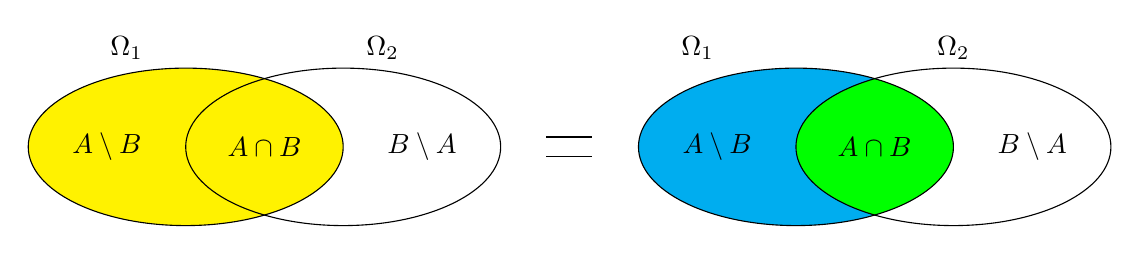
\begin{tikzpicture}[scale=0.5]
\begin{scope}
  \fill[yellow] (-3.5,1.5) ellipse (4 and 2);
\end{scope}
\begin{scope}
  \fill[cyan] (12,1.5) ellipse (4 and 2);
\end{scope}
\begin{scope}
  \clip (12,1.5) ellipse (4 and 2);
  \fill[green] (16,1.5) ellipse (4 and 2);
\end{scope}
%%
\draw (-3.5,1.5) ellipse (4 and 2);
\draw (0.5,1.5) ellipse (4 and 2);
\node at (-5.5,1.5) {$A\setminus B$};
\node at (-1.5,1.5) {$A\cap B$};
\node at (2.5,1.5) {$B\setminus A$};
\node at (-5,4) {$\Omega_1$};
\node at (1.5,4) {$\Omega_2$};
%% 
\draw (5.66,1.75) -- (6.82,1.75);
\draw (5.66,1.25) -- (6.82,1.25);
%%
\draw (12,1.5) ellipse (4 and 2);
\draw (16,1.5) ellipse (4 and 2);
\node at (10,1.5) {$A\setminus B$};
\node at (14,1.5) {$A\cap B$};
\node at (18,1.5) {$B\setminus A$};
\node at (9.5,4) {$\Omega_1$};
\node at (16,4) {$\Omega_2$};
\end{tikzpicture}
\end{center}

\br
As noted before, it suffices to know $P\big((-\infty,\lambda]\big)$ for all $\lambda \in \R$, and for this reason a new notation is introduced; \bse
P(\lambda) := P\big((-\infty,\lambda]\big).
\ese 
However, as they are written they appear to have different domains. We therefore give a new name to $P(\lambda)$; the \emph{resolution of the identity}\index{resolution of the identity}. 
\er

\subsection{Real and Complex Valued Borel Measures Induced by a PVM}

\bd 
For all $\psi,\varphi\in\cH$ we define the $\C$-valued measure 
\bi{rrCl}
\mu_{\psi,\varphi} \cl & \sigma(\cO_{\R}) & \to & \C\\
& \Omega  & \mapsto & \mu_{\psi,\varphi}(\Omega) := \braket{\psi}{P(\Omega)\varphi}.
\ei
\ed 

\bd 
For all $\psi\in\cH$ we define the $\R$-valued measure
\bse 
\mu_{\psi} := \mu_{\psi,\psi}
\ese 
\ed 

\bq that $\mu_{\psi}(\Omega)\in\R$. 
\bi{rCl}
\mu_{\psi}(\Omega) & = & \braket{\psi}{P(\Omega)\psi} \\
& = & \braket{P(\Omega)\psi}{\psi} \\
& = & \overline{\braket{\psi}{P(\Omega)\psi}} \\
& = & \overline{\mu_{\psi}(\Omega)},
\ei 
where we have used the fact that $P$ is self adjoint to go from the first to the second line. 
\eq

\subsection{Integration With Respect to a PVM}

We now wish to make sense of the operator $\int_{\R}fdP$ for measurable $f:\R\to\C$. We will build this up in three steps: 

\ben[label=(\roman*)]
\item For simple $f$, 
\item For bounded $f$, and 
\item For not necessarily bounded\footnote{Recall footnote 5 from lecture 2: to us the term `unbounded' means definitely \textit{not} bounded.} $f$. 
\een 

\br 
As we shall see, if $f$ is bounded (in the sense that there exists a $a\in\R$ such that $|f(x)|<a$ for all $x\in\R$) that the integral part of the operator will have nice properties. For example it will be linear in $f$, i.e. 
\bse 
\int_{\R}(\alpha f + g) dP = \alpha \int_{\R}fdP + \int_{\R}gdP,
\ese 
for $\alpha\in\C$. However, if $f$ is unbounded, domain issues will destroy the equality above. It is important to note, though, that it is exactly the latter case we need as 
\bi{rrCl}
f= i_{\R} \cl & \R & \hookrightarrow & \C\\
& x & \mapsto & x 
\ei 
in the Spectral theorem, which is clearly unbounded. 
\er 

\subsubsection*{A. \ Simple $f$}

Recall a simple function is a measurable function that takes a finite number of results in the target, i.e. if $f\cl\R\to\C$ then
\bse
f(\R) = \{f_1,...,f_N\} \ss \C
\ese 
for some $N\in\N$. This allows us to rewrite $f$ as
\bse 
f = \sum_{n=1}^N f_n \chi_{\Omega_n},
\ese 
where $\Omega_n := \preim_f(\{f_n\})$ and $\chi$ is the characteristic function.

\bd 
For simple $f:\R\to\C$ and PVM $P$ we define 
\bse
\int_{\R}fdP := \sum_{n=1}^Nf_nP(\Omega_n).
\ese 
\ed 

\bp 
For simple $f$, $\int_{\R}fdP$ is linear in $f$.
\ep 

\bq 
Let $S(\R,\C)$ denote the set of all simple functions $f:\R\to\C$. We can make this set into a $\C$-vector space by inheriting the addition and $s$-multiplication from $\C$, namely define 
\bse
(f+g)(x) := f(x) + g(x), \qquad (\alpha\cdot f)(x) := \alpha\cdot f(x),
\ese 
for all $f,g\in S(\R,\C)$, $\alpha\in\C$. 

Now consider the preimage part: As $f$ and $g$ are both simple it follows that 
\bse 
(f+g)(x) = f_n + g_n 
\ese 
for some $f_n,g_n\in\C$, so the preimage term becomes
\bi{rCl}
\preim_{f+g}\{f_n+g_n\} = \{x\} & = & \preim_{f}\{f_n\} \\
& = & \preim_{g}\{g_n\}.
\ei
It follows trivially, then, that 
\bse 
\int_{\R} (f+g)dP = \int_{\R}fdP + \int_{\R}gdP.
\ese 

A similar method gives the $\alpha\in\C$ condition of linearity. 
\eq 

\br 
\label{rmk:CharacteristicPVM}
Observe that $\chi_{\Omega}$ for any $\Omega\in\sigma(\cO_{\R})$ is simple (it only takes the values 0 or 1), and hence 
\bse
\int_{\R}\chi_{\Omega} dP = 1\cdot P(\Omega) + 0\cdot P(\sigma\setminus\Omega) = P(\Omega).
\ese 
\er 

\br
Observe also that for any $\psi,\varphi\in\cH$, 
\bi{rCl}
\braket{\psi}{\bigg(\int_{\R}fdP\bigg)\varphi} & = & \braket{\psi}{\sum_{n=1}^N f_n P(\Omega_n) \varphi} \\
& = & \sum_{n=1}^Nf_n \braket{\psi}{P(\Omega_n)\varphi} \\
& = & \sum_{n=1}^N f_n \mu_{\psi,\varphi}(\Omega_n) \\
& =: & \int_{\R} f d\mu_{\psi,\varphi},
\ei 
where \Cref{prp:MeasureIntegral} was used.
\er 

\bd 
For simple $f$ we can define the map 
\bi{rrCl}
\bigg(\int_{\R}dP\bigg) \cl & S(\R,\C) & \to & \cL(\cH) \\
& f & \mapsto & \int_{\R}fdP,
\ei 
which, if we equip $S(\R,\C)$ with the suppremum norm and $\cL(\cH)$ with its operator norm, has operator norm $\|\int_{\R}dP\| = 1$.
\ed 

\bq 
We have already shown that $\int_{\R}fdP \in\cL(\cH)$ (i.e. it is linear), so we just need to show the norm condition. First, let $f\in S(\R,\C)$ and $\psi\in\cH$, then
\bi{rCl}
\bigg{\|}\bigg(\int_{\R}fdP\bigg)\psi\bigg{\|}_{\cH}^2 & = & \braket{\bigg(\int_{\R}fdP\bigg)\psi}{\bigg(\int_{\R}fdP\bigg)\psi} \\
& = & \braket{\sum_{n=1}^Nf_nP(\Omega_n)\psi}{ \sum_{m=1}^Nf_m P(\Omega_m) \psi} \\
& = & \braket{\psi}{ \sum_{n,m=1}^N \overline{f_n} f_m P(\Omega_n) P(\Omega_m) \psi} \\
& = & \braket{\psi}{\sum_{n,m=1}^N \overline{f_n} f_m \delta_{nm} P(\Omega_m) \psi} \\
& = & \sum_{n=1}^N |f|^2 \braket{\psi}{P(\Omega_n)\psi} \\
& = & \sum_{n=1}^N |f|^2 \mu_{\psi}(\Omega_n) \\
& =: & \int_{\R} |f|^2 d\mu_{\psi} \\
\implies \bigg{\|}\bigg(\int_{\R}fdP\bigg)\psi\bigg{\|}_{\cH} & \leq & \|f\|_{\infty}\|\psi\|_{\cH},
\ei 
where we have used the definition of the norm in terms of the inner product, the fact that $P$ is self adjoint, the fact that $P(\Omega_n)P(\Omega_m) = \delta_{nm}$ for pairwise disjoint $\Omega_n/\Omega_m$, and \Cref{prp:NormLp} along with the fact that $\|f\|_{\infty} := \sup_{x\in\R}f(x)$. The equality in the last line can be assumed provided $f$ and $\psi$ are sufficiently chosen. 

Thus we have 
\bi{rCl}
\bigg{\|} \int_{\R}dP\bigg{\|} & := & \sup_{f\in S(\R,\C)}  \frac{\big{\|}\int_{\R}fdP\big{\|}_{\cL(\cH)}}{\|f\|_{\infty}} \\
& := & \sup_{f\in S(\R,\C)} \sup_{\psi\in\cH} \frac{\big{\|}\big(\int_{\R}fdP\big)\psi\big{\|}_{\cH}}{\|f\|_{\infty}\|\psi\|_{\cH}} \\
& = & 1.
\ei 
\eq 

\subsubsection*{B. \ Bounded Borel Functions}

\bd 
The set of all bounded, measurable functions is denoted 
\bse 
\cB(\R,\C) := \{f\cl\R\to\C \,|\, \text{measurable}, \|f\|_{\infty} <\infty\}.
\ese
\ed 

\bp 
The set $\cB$ can be made into a Banach space by defining the norm 
\bse 
\|f\|_{\cB} := \sup_{x\in\R} |f(x)|.
\ese 
\ep 

\bq 
We turn the set into a linear vector space in the usual manner; we inherit the addition and $s$-multiplication from $\C$. 

Now prove $\|f\|_{\cB}$ is a norm. Comparing to the definition given at the bottom of Page 9, for $f,g\in\cB(\R,\C)$ and $z\in\C$ we have 
\ben[label=(\roman*)]
\item Clearly $\|f\|_{\cB} \geq 0$.
\item 
\bi{rCl}
\|f\|_{\cB} & = &  0 \\ 
\eqv \sup_{x\in\R}|f(x)| & = & 0 \\
\eqv f(x) & = & 0 \qquad \forall x\in\R
\ei 
so $f=0$. 
\item 
\bi{rCl}
\|z\cdot f\|_{\cB} & := & \sup_{x\in\R}|z\cdot f(x)| \\
& = & |z|\sup_{x\in\R}|f(x)| \\
& =: & |Z|\cdot \|f\|_{\cB}.
\ei 
\item 
\bi{rCl}
\|f+g\|_{\cB} & := & \sup_{x\in\R} |(f+g)(x)| \\
& = & \sup_{x\in\R}|f(x)+g(x)| \\
& \leq &  \sup_{x\in\R}|f(x)|+ \sup_{x\in\R}|g(x)| \\
& =: & \|f\|_{\cB} + \|g\|_{\cB}.
\ei
\een

Now let $\{f_n\}_{n\in\N}$ be a Cauchy sequence in $\cB(\R,\C)$, that is: $\forall \epsilon>0, \exists N\in\N \cl \forall m,n\geq N$ we have 
\bse 
d(f_n,f_m) := \|f_n - f_m\|_{\cB} := \sup_{x\in\R} |f_n(x)-f_m(x)| < \epsilon.
\ese 

Now from the definition of the supremum we have 
\bse 
|f_n(x) - f_m(x)| \leq \|f-g\|_{\cB},
\ese 
so it follows that the sequence $\{f_n(x)\}_{n\in\N}$ is a Cauchy sequence in $\C$. But $\C$ is a complete metric space so we know that this Cauchy sequence converges in $\C$, i.e. 
\bse 
\lim_{n\to\infty} f_n(x) = z_x \in \C.
\ese 
We can thus define a point-wise limit $f$ of the sequence $\{f_n\}_{n\in\N}\ss \cB(\R,\C)$ as
\bse 
f(x) := \lim_{x\to\infty} f_n(x) = z_x
\ese 
for all $x\in\R$. Then, by equipping $\C$ and $\R$ with their respective Borel $\sigma$-algebras, \Cref{prp:MeasurablePointwiseLimit} tells us that $f$ is measurable. 

Finally from the fact that $\cB(\R,\C) \ss \cL(\R,\C)$, \Cref{thrm:BoundedLinearOperatorsBanach} tells us that $f$ is bounded and so $\cB(\R,\C)$ is a Banach space. 
\eq 

\bc
Observe that $S(\R,\C)$ is in-fact a dense, linear subspace of $\cB(\R,\C)$. Thus, the BLT theorem tells us that we have a unique extension of the operator 
\bse 
\bigg(\int_{\R}dP\bigg) \cl S(\R,\C) \to \cL(\cH)
\ese 
to the domain $\cB(\R,\C)$ with equal operator norm. That is, we have an operator 
\bse 
\widehat{\bigg(\int_{\R}dP\bigg)} \cl \cB(\R,\C) \to \cL(\cH)
\ese 
with $\big{\|}\widehat{\int_{\R}dP}\big{\|}=1$. 
\ec 

\bc 
By suitable definition we can turn the space $\cB(\R,\C)$ into an $C^*$-algebra and our operator then has the following properties 
\ben[label=(\roman*)]
\item \bse 
\int_{\R} 1 dP = \id_{\cH} 
\ese 
\item \bse 
\int_{\R}(f\cdot g)dP = \bigg(\int_{\R}fdP\bigg) \circ \bigg(\int_{\R}gdP\bigg)
\ese 
\item \bse 
\int_{\R}\overline{f}dP = \bigg(\int_{\R}fdP\bigg)^*
\ese
\een
These properties collectively make the operator a $C^*$-algebra homomorphism.
\ec 

\subsubsection*{C. \ General Borel Function}

We now want to allow for the case that $f$ is unbounded. We will write the following such that it reduces to the above when $f$ is bounded. 

\bd 
Let $f:\R\to\C$ be measurable, then we define the linear map 
\bse 
\bigg(\int_{\R} fdP\bigg) \cl \cD_{\int_{\R}fdP} \to \cH
\ese 
where 
\bse 
\cD_{\int_{\R}fdP} := \bigg{\{}\psi\in\cH \,\Big{|}\, \int_{\R}|f|^2 d\mu_{\psi} < \infty\bigg{\}} \se \cH,
\ese 
is a dense, linear subspace. The linear map is defined via 
\bse 
\bigg(\int_{\R}fdP\bigg)\psi := \lim_{n\to\infty} \bigg[\bigg(\int_{\R}f_ndP\bigg)\psi\bigg],
\ese
where the sequence $\{f_n\}_{n\in\N}\se \cB(\R,\C)$ defined by 
\bse 
f_n := \chi_{\{x\in\R|f(x)<n\}} f.
\ese 
\ed 

\br 
Note that the map above includes the $f$, it is not just the integral defined in the previous section. Note also for the case when $f\in\cB(\R,\C)$ we just recover the case above and we have $\cD_{\int_{\R}fdP}=\cH$ (i.e. we have $\cL(\cH)$). Otherwise it is a proper  subset.
\er 

\br 
The literature often introduces the notation 
\bse 
\cD_f := \cD_{\int_{\R}fdP},
\ese 
however this could lead one to think of the domain of $f$ itself, which here is $\R$. We will avoid this notation.
\er 

\br
The sequence $\{f_n\}_{n\in\N}$ can be thought of as `chopping' $f$ into bounded parts. 

\begin{center}
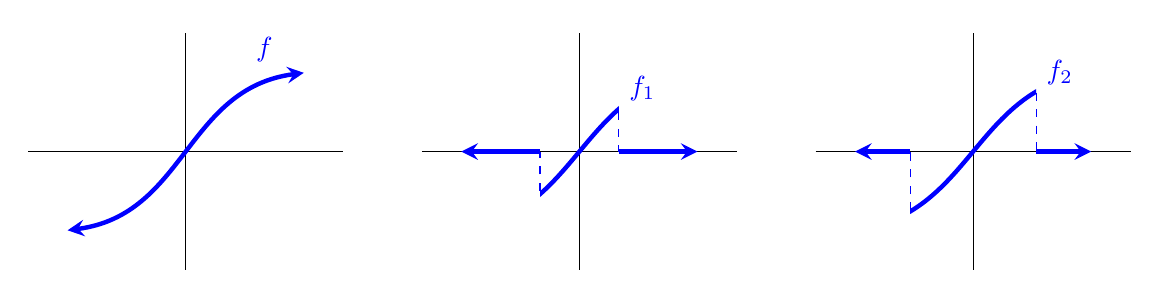
\begin{tikzpicture}
\draw (-10,0) -- (-6,0);
\draw (-8,-1.5) -- (-8,1.5);
\draw[blue, ultra thick, <->] (-9.5,-1) .. controls (-8, -0.8) and (-8,0.8) .. (-6.5,1);
\node at (-7,1.3) {\textcolor{blue}{$f$}};
%%
\draw (-5,0) -- (-1,0);
\draw (-3,-1.5) -- (-3,1.5);
\begin{scope}
  \clip (-3.5, 1.5) rectangle (-2.5,-1.5);
  \draw[blue, ultra thick] (-4.5,-1) .. controls (-3, -0.8) and (-3,0.8) .. (-1.5,1);
\end{scope}
\draw[blue, dashed] (-3.5,-0.5) -- (-3.5,0);
\draw[blue, dashed] (-2.5,0.5) -- (-2.5,0);
\draw[blue, ultra thick, ->]  (-3.5,0) -- (-4.5,0); 
\draw[blue, ultra thick, ->] (-2.5,0) -- (-1.5,0);
\node at (-2.2,0.8) {\textcolor{blue}{$f_1$}};
%% 
\draw (0,0) -- (4,0);
\draw (2,-1.5) -- (2,1.5);
\begin{scope}
  \clip (1.2, 1.5) rectangle (2.8,-1.5);
  \draw[blue, ultra thick] (0.5,-1) .. controls (2, -0.8) and (2,0.8) .. (3.5,1);
\end{scope}
\draw[blue, dashed] (1.2,-0.75) -- (1.2,0);
\draw[blue, dashed] (2.8,0.75) -- (2.8,0);
\draw[blue, ultra thick, ->] (1.2,0) -- (0.5,0);
\draw[blue, ultra thick, ->] (2.8,0) -- (3.5,0);
\node at (3.1,1) {\textcolor{blue}{$f_2$}};
\end{tikzpicture}
\end{center}
\er 

\bl 
The sequence $\{f_n\}_{n\in\N}$ is Cauchy in $L^2(\R)$. This in tern implies that the sequence $\{(\int_{\R}f_ndP)\psi\}_{n\in\N}$ is Cauchy in $\cH$, which is required for the limit in the definition to make sense, i.e. the result lies in $\cH$.
\el 

For this general case of a measurable $f$ we have:
\ben[label=(\roman*)]
\item As before
\bse 
\int_{\R}\overline{f}dP = \bigg(\int_{\R}fdP\bigg)^*.
\ese 
\item For $\alpha\in\C$ and $f,g$ measurable,
\bse 
\bigg(\alpha \int_{\R}fdP + \int_{\R}gdP \bigg) \se \int_{\R}(\alpha f + g)dP,
\ese 
where the equality holds only for bounded $f$. As explained earlier, the inequality arises due to domain issues. We can now see this more explicitly from the definition of $\cD_{\int_{\R}fdP}$; just because $f$ and $g$ are both measurable, it does not mean that their respective map domains will coincide. However, the domain for the LHS is $\cD_{\int_{\R}(|\alpha f| + |g|)dP}$.
\item \bse 
\bigg(\int_{\R}fdP\bigg)\circ \bigg(\int_{\R}gdP\bigg) \se \int_{\R}(f\cdot g)dP,
\ese 
again where the equality holds only when $f$ and $g$ are bounded.
\een

\subsection{The Inverse Spectral Theorem}

We are now in a place where we can understand the inverse spectral theorem. 

\bd 
Given a PVM, $P$, we can construct a self adjoint operator $A_P$ as 
\bse 
A_P := \int_{\R} \id_{\R} dP,
\ese 
where $\id_{\R}\cl \R\hookrightarrow \C$ is the inclusion map. 
\ed 

\bq 
\bi{rCl}
(A_P)^* & = & \int_{\R} \overline{\id_{\R}} dP \\
& = & \int_{\R} \id_{\R} dP \\
& = & A_P,
\ei 
so $A_P$ is self adjoint. 
\eq 
\newpage

\section{Spectral theorem}
The inverse spectral theorem tells us how to construct a self adjoint operator $A_P$ given a projection valued measure $P$. The aim of this lecture is to do the opposite; given a self adjoint operator $A$ we want to find a PVM $P_A$. We want the two methods to be in unison --- that is we want $A_{P_A} = A$ and $P_{A_P} = P$. We shall start by assuming that $A$ can be written in integral form, and then shall remove this restriction.

\subsection{Measurable Function Applied To A Spectrally Decomposable Self Adjoint Operator}

The term \textit{spectrally decomposable} means that is has integral form. 

\bd 
Let the self adjoint operator $A$ be \emph{spectrally decomposable}; i.e. there exists a PVM $P$ such that 
\bse 
A = \int_{\R} \id_{\R} dP,
\ese 
then for any measurable function $f:\R\to\C$, we define the operator 
\bse 
f(A) \cl \cD_{\int fdP} \to \cH,
\ese 
given by
\bse 
f(A) := \int_{\R} (f\circ \id_{\R} )dP \equiv \int_{\R} f(\lambda) P(d\lambda).
\ese 
\ed 

\br 
The spectral theorem will show that every self adjoint operator $A$ is spectrally decomposable by virtue of a uniquely detemerined $P$.
\er 

\bc 
If $f\cl \R \to \R$, then $f(A)$ is again self adjoint. 
\ec 

\bq 
\bi{rCl}
[f(A)]^* & := & \bigg[\int_{\R} (f\circ \id_{\R} )dP\bigg]^* \\
& = & \int_{\R} (\overline{f} \circ \id_{\R})dP \\
& = & \int_{\R} fdP \\
& =: & f(A).
\ei 
\eq 

Let us now consider two important examples.
\be 
\label{ex:ExpSpectral}
Let $A=\int_{\R}\lambda P(d\lambda)$ be self adjoint. Then
\bse 
\exp(A) := \int_{\R} e^{\lambda} P(d\lambda)
\ese
is self adjoint due to the previous Corollary. However 
\bse 
\exp(iA) := \int_{\R} e^{i\lambda} P(d\lambda)
\ese 
is \emph{not} self adjoint. This latter case is of high importance in QM, as can be seen by revisiting Axiom 4 at the start. 
\ee 

\be 
Let $A=\int_{\R}\lambda P(d\lambda)$ be self adjoint and $\Omega\in\sigma(\cO_{\R})$. Then
\bse
P(\Omega) = \int_{\R} \chi_{\Omega} dP
\ese
implies 
\bi{rCl}
\sq \big(P(\Omega)\big) & := & \int_{\R} (\sq \circ \chi_{\Omega} dP \\ 
& \equiv & \int_{\R} [\chi_{\Omega}(\lambda)]^2 P(d\lambda) \\
& = & \int_{\R} \chi_{\Omega}(\lambda) P(d\lambda) \\
& = & P(\Omega),
\ei 
which is one of the projection conditions.
\ee 

\subsection{Reconstruct PVM From a Spectrally Decomposable, Self Adjoint Operator}

The key to reconstructing the associated PVM $P$ is to consider the resolvents. 

\bd
Given a spectrally decomposable operator $A$ and an the resolvant set $\rho(A)$, we define
\bse 
r_z(A) = R_Z(A) := (A-z\id_{\cH})^{-1},
\ese 
which is rewritten as
\bi{rrCl}
r_z \cl & \R & \to & \C \\
& \lambda & \mapsto & \frac{1}{\lambda -z},
\ei 
and, due to the fact that $A$ is spectrally decomposable, satisfies 
\bse 
r_z(A) = \int_{\R} (r_z\circ \id_{\R})dP \equiv \int_{\R} \frac{1}{\lambda-z}P(d\lambda).
\ese 
\ed 

Note, using the results in the previous lecture, we have that for any $\psi\in\cH$,
\bi{rCl}
\braket{\psi}{R_A(z)\psi} & = & \braket{\psi}{ \bigg(\int_{\R}(r_z\circ\id_{\R})dP\bigg)\psi} \\
& = & \int_{\R} (r_z\circ\id_{\R} )d\mu_{\psi} \\
& \equiv & \int_{\R} \frac{1}{\lambda - z} \mu_{\psi}(d\lambda).
\ei 

\bd 
A \emph{Herglotz function} is an analytic complex function that maps the upper half plane into itself, but need not be surjective or injective. They are also known as \emph{Nevanlinna/Pick/R} functions. 
\ed 

\bt 
The function 
\bi{rrCl}
\braket{\psi}{R_A(\cdot) \psi}  \cl & \C & \to & \C \\
& z & \mapsto & \int_{\R} \frac{1}{\lambda -z} \mu_{\psi} (d\lambda)
\ei 
is Herglotz.
\et 

\bq 
Recall
\bse 
\mu_{\psi}\cl\sigma(\cO_{\R})\to\R^+_0
\ese 
is real-valued. Then using 
\bse 
\Im{(r)} = \frac{1}{2}(r-\overline{r}),
\ese 
we have 
\bi{rCl}
\Im{\braket{\psi}{R_A(z)\psi}} & = & \int_{\R} \Im\bigg(\frac{1}{\lambda - z}\bigg) \mu_{\psi}(d\lambda) \\
& = & \frac{1}{2}\int_{\R}\bigg[ \frac{1}{\lambda-z} - \frac{1}{\lambda -\overline{z}}\bigg] \mu_{\psi}(d\lambda) \\
& = & \int_{\R} \frac{z-\overline{z}}{2|\lambda-z|^2}\mu_{\psi} (d\lambda) \\
& = & \Im(z)  \int_{\R} \frac{1}{|\lambda-z|^2} \mu_{\psi}(d\lambda).
\ei 
Then, since the fact that the integral is Lebesgue and the intergrand is non-negative and so 
\bse
\Im\braket{\psi}{R_A(z)\psi} > 0 \quad \Leftrightarrow \quad  \Im(z) > 0.
\ese 
\eq 

Recalling the start of last lecture, if we can find a way to construct $\mu_{\psi}$ from our $A$ then we can use that to reconstruct $P$. The result of this is the previously mentioned Stieltjes Inversion Formula, and it is obtained as follows. 

Let $t,\epsilon\in\R$. Then, since $A$ is self adjoint and so its spectrum is purely real, $t+i\epsilon\in\rho(A)$. This allows us to act on it with $R_A$. Thus, consider 
\bi{rCl} 
\lim_{\varepsilon\to 0^+} \frac{1}{\pi}\int_{t_1}^{t_2}dt \Im\braket{\psi}{R_A(t+i\varepsilon)\psi} & = & \lim_{\varepsilon\to0^+} \frac{1}{\pi} \int_{t_1}^{t_2}dt \int_{\R} \frac{\varepsilon}{|\lambda-t-i\varepsilon|^2}\mu_{\psi}(d\lambda) \\
& = & \lim_{\varepsilon\to0^+} \int_{\R} \bigg( \frac{1}{\pi} \int_{t_1}^{t_2}dt \frac{\varepsilon}{(\lambda-t)^2 +\varepsilon^2}\bigg)\mu_{\psi}(d\lambda), 
\ei
where Fubini's Theorem\footnote{See  \href{https://en.wikipedia.org/wiki/Fubini\%27s_theorem}{Wiki}} has been used. The inner integral is a standard integral, with result
\bse
\frac{1}{\pi} \int_{t_1}^{t_2} dt \frac{\varepsilon}{(\lambda-t)^2+\varepsilon^2} = \frac{1}{\pi}\bigg[ \arctan\bigg(\frac{t-\lambda}{\varepsilon}\bigg)\bigg]^{t_2}_{t_1}.
\ese 
Now strictly, at this stage, we cannot simply pull the $\varepsilon$ limit into this expression; we would need to check that the above result is bounded first and then, by dominated convergence, we can pull it in. This will turn out to be true, and so in order to simplify the following we consider $\varepsilon$ to be small here. 

In order to work out the above expression, we can use the $\lambda$-graphs. Let's plot both terms (including the overall minus sign that comes with $t_1$) on the same graph: 

\begin{tikzpicture}
\begin{axis}[
    domain=-10:10,
    xscale=1.5,yscale=1,
    xmin=0, xmax=10,
    ymin=-2, ymax= 2,
    samples=1000,
    axis lines=center,
    xticklabels={},
    yticklabels={},
]
    \addplot+[mark=none] {rad(atan((7-x)/(0.1))};
    \addplot+[mark=none] {-rad(atan((3-x)/(0.1))};
\end{axis}
\node at (-0.35,0.7) {$-\frac{1}{2}$};
\node at (-0.3,5) {$\frac{1}{2}$};
\node at (3.3,2.6) {$t_1$};
\node at (7.5,2.6) {$t_2$};
\node at (10,2.6) {$\lambda$};
\node at (11.5,4.8) {\textcolor{red}{$-\frac{1}{\pi}\arctan\big(\frac{t_1-\lambda}{\varepsilon}\big)$}};
\node at (11.5,1) {\textcolor{blue}{$\frac{1}{\pi}\arctan\big(\frac{t_2-\lambda}{\varepsilon}\big)$}};
\end{tikzpicture}

Taking the limit and adding gives 

\begin{tikzpicture}
\begin{axis}[
    domain=-10:10,
    xscale=1.5,yscale=1,
    xmin=0, xmax=10,
    ymin=0, ymax= 2,
    samples=1000,
    axis lines=center,
    xticklabels={},
    yticklabels={},
]
\end{axis}
\node at (-0.35,4.3) {$1$};
\node at (-0.35,2.15) {$\frac{1}{2}$};
\node at (-0.35,0) {$0$};
\node at (3.3,-0.35) {$t_1$};
\node at (7.5,-0.35) {$t_2$};
\node at (10,-0.35) {$\lambda$};
\draw[blue, ultra thick] (0,0) -- (3.3,0);
\draw[blue, ultra thick] (3.3,4.3) -- (7.5,4.3);
\draw[blue, ultra thick] (7.5,0) -- (10,0);
\draw[blue] (3.3,0) circle (3pt);
\filldraw[blue] (3.3,2.15) circle (3pt);
\draw[blue] (3.3,4.3) circle (3pt);
\draw[blue] (7.5,4.3) circle (3pt);
\filldraw[blue] (7.5,2.15) circle (3pt);
\draw[blue] (7.5,0) circle (3pt);
\end{tikzpicture}

So we have
\bse 
\lim_{\varepsilon\to0^+} \frac{1}{\pi}\int_{t_1}^{t_2} dt \frac{\varepsilon}{(\lambda-t)^2+\varepsilon^2} = \frac{1}{2}\big( \chi_{(t_1,t_2)} + \chi_{[t_1,t_2]} \big),
\ese 
and 
\bse 
\lim_{\varepsilon\to0^+} \frac{1}{\pi}\int_{t_1}^{t_2}dt \Im\braket{\psi}{R_A(t+i\varepsilon)\psi} = \frac{1}{2} \int_{\R} \big(\chi_{(t_1,t_2)} + \chi_{[t_1,t_2]} \big)\mu_{\psi}(d\lambda).
\ese 

Finally, we have the Stieltjes Inversion Formula. 

\bt[Stieltjes Inversion Formula] 
Given a spectrally decomposable, self adjoint operator $A$ and its associated resolvent map $R_A$, we can construct a real-valued measure
\bse 
\mu^A_{\psi}\big((-\infty,\lambda] \big) = \lim_{\delta\to0^+}\lim_{\varepsilon\to0^+}\frac{1}{\pi} \int_{-\infty}^{\lambda+\delta} dt \Im\braket{\psi}{R_A(t+i\varepsilon)\psi}. 
\ese 
\et 

\bq 
\bi{rCl}
\lim_{\delta\to0^+}\lim_{\varepsilon\to0^+}\frac{1}{\pi} \int_{-\infty}^{\lambda+\delta} dt \Im\braket{\psi}{R_A(t+i\varepsilon)\psi} & = & \lim_{\delta\to0^+} \frac{1}{2}\int_{\R} \big(\chi_{(-\infty,\lambda+\delta)} + \chi_{(-\infty,\delta]} \big)\mu_{\psi}(d\lambda) \\
& = & \int_{\R} \chi_{(-\infty,\lambda]}\mu_{\psi}(d\lambda) \\
& = & \mu_{\psi}\big((-\infty,\lambda]),
\ei
where we used the fact that the $\chi(\Omega)$ is bounded to move the limit inside the integral along with the fact that 
\bse 
\lim_{\delta\to0^+} (-\infty,\lambda+\delta) = (-\infty,\lambda].
\ese 
\eq 

\br 
Note the fact that $\braket{\psi}{R_A(t+i\varepsilon)\psi}$ is Herglotz with the fact that $\varepsilon>0$ gives us that $\mu_{\psi}^A \geq 0$, which is required for it to be a real-valued measure. 
\er 

\br
If we already know that $A$ is spectrally decomposable w.r.t. some PVM $P$, then we can recover $P$ from $A$ by virtue of: for any $\Omega\in\sigma(\cO_{\R})$ and for all $\psi,\varphi\in\cH$
\bse 
\braket{\psi}{P(\Omega)\varphi} = \int_{\R} \chi_{\Omega} d\mu_{\psi,\varphi},
\ese 
where $\mu_{\psi,\varphi}$ is obtained from $\mu_{\psi}$ using the method given at the start of the previous lecture.
\er

\subsection{Construction Of PVM From A Self Adjoint Operator}

We need to free ourselves from the fact that $A$ is known to be spectrally decomposable from the start. We could do this by trying to recreate the above method, i.e. arrive at the Stieltjes Inversion Formula for an operator $A$, by showing that 

\ben[label=(\roman*)]
\item $\braket{\psi}{R_A(\cdot)\psi} : \C \to \C$ is Herglotz for any self adjoint $A$
\item $\braket{\psi}{P(\Omega)\varphi} := \int_{\R}\chi_{\Omega}d\mu_{\psi,\varphi}$ is indeed a PVM.
\een 

In order to prove these we first need a new theorem. 
\bt[First-Resolvent Formula]
For any operator $A:\cD_{A}\to\cH$ and $a,b\in\rho(A)$ we have 
\bse 
R_A(a)-R_A(b) = (a-b)R_A(a)R_A(b) = (a-b)R_A(b)R_A(a).
\ese 
\et 

\bq
Consider 
\bi{rCl}
R_A(a) - (a-b)R_A(a)R_A(b) & := & (A-a)^{-1} - (a-b)(A-a)^{-1}(A-b)^{-1} \\
& = & (A-a)^{-1}\big[\id_{\cH} - (a-b)(A-b)^{-1}\big] \\
& = & (A-a)^{-1}\big[\id_{\cH} - (a-A+A-b)(A-b)^{-1}\big] \\
& = & (A-a)^{-1} \big[\id_{\cH} +(A-a)(A-b)^{-1} - (A-b)(A-b)^{-1}\big] \\
& = & (A-b)^{-1} \\
& = & R_A(b),
\ei 
and similarly for the the other result. 
\eq 


Conclusion, the Spectral Theorem, \Cref{thm:Spectral}, together with the recipe for the construction of the PVM $P$ from a self adjoint operator $A$ holds. 

\subsection{Commuting Operators}

The study of QM is teaming with so called \emph{commutators}. However, they are not as simply defined as is often erroneously assumed. In particular, the commutator between the position and momentum given by 
\bse 
[Q^i,P_j] = i\hbar {\delta^i}_j
\ese 
is not even defined, unless further provisions are given. This formula appears in the opening sections of almost all QM textbooks though, and so it's important we understand what is meant. 

One can happily write the commutator provided the operators involved are bounded (which from the lecture 9 we see that at least $P_j$ is not).

\bd 
Let $B_1,B_2\in\cL(\cH)$, i.e. they are bounded linear operators from $\cH$ to $\cH$. Then one may define 
\bse 
[B_1,B_2] := B_1\circ B_2 - B_2\circ B_1,
\ese 
where 
\bse 
[B_1,B_2] \in \cL(\cH).
\ese 
\ed 

\br 
The tuple $(\cL(\cH),+,\cdot,[\cdot,\cdot])$ is a Lie algebra\footnote{See Dr. Schuller's Lectures on the Geometric Anatomy of Theoretical Physics}.
\er 

\bc 
\label{cor:ABCCommutator}
Let $A,B,C\in\cL(\cH)$ then the following holds 
\bse 
[A\circ B,C] = [A,C]\circ B + A\circ[B,C].
\ese 
\ec 

\bq 
Consider the action on some arbitrary $\psi\in\cH$. 
\bi{rCl}
[A\circ B,C]\psi & := & (A\circ B)\circ (C\psi) - C\circ(A\circ B\psi) \\
& = & A \circ (B\circ C\psi) - C\circ(A\circ B\psi) \\
& = & A \circ (C\circ B \psi + [B,C]\psi) - C\circ(A\circ B\psi) \\
& = & (A \circ C) \circ B \psi + A\circ [B,C]\psi - C\circ(A\circ B\psi) \\
& = & (C\circ A + [A,C])\circ B\psi + A\circ [B,C]\psi - C\circ(A\circ B\psi) \\
& = & [A,C]\circ B\psi + A\circ[B,C]\psi \\
& = & ([A,C]\circ B + A\circ[B,C])\psi,
\ei 
where we used the associativity of the composition of maps. Then, as $\psi$ was arbitrary, we have our result. 
\eq 

\bc 
Let $A$ and $B$ be two operators. Then if one of the them is unbounded the domain $\cD_{[A,B]}$ may only have a trivial definition, i.e. $\cD_{[A,B]} = \{0_{\cH}\}$.
\ec 

\bq
Let $A:\cD_A\to\cH$ be unbounded with $\cD_A \ss \cH$, and define the bounded operator
\bi{rrCl}
B_{\varphi} : & \cH & \to & \cH \\
& \alpha & \mapsto & \braket{\varphi}{\alpha} \psi =: \ell_{\varphi}(\alpha) \psi
\ei 
for some fixed $\varphi,\psi\in\cH$ where $\psi\notin\cD_A$. So we have $\ran(B_{\varphi}) = \cH\setminus\cD_A$. Then from the first term in
\bse
[A,B_{\varphi}] := A\circ B_{\varphi} - B_{\varphi}\circ A,
\ese
it follows that 
\bse 
\cD_{[A,B_{\varphi}]} = \ran(B_{\varphi})\cap \cD_{A} = \{0_{\cH}\}.
\ese 
\eq 

\bd 
Two bounded linear operators $A,B\in\cL(\cH)$ are said to \emph{commute} if 
\bse 
[A,B] = 0.
\ese 
\ed 

\bc 
Let $A,B\in\cL(\cH)$ be commuting operators. Then if $A$ is also non-degenerate then any $\psi$ that is an eigenvector of $A$ is also an eigenvector of $B$. In other words, the set of $A$'s eigenvectors is contained within the set of $B$'s. 
\ec 

\bq 
Let $\psi\in\cD\setminus\{0\}$ be an eigenvector of $A$ with eigenvalue $\lambda\in\C$. Then we have 
\bi{rCl}
[A,B]\psi & := & (A\circ B - B\circ A)\psi \\
& = & A(B\psi) - B(A\psi) \\
& = & A(B\psi) - \lambda B(\psi),
\ei 
where we have used the fact that $B$ is linear. Then from the fact that $[A,B]=0$ it follows that $B\psi$ is also an eigenvalue of $A$ with eigenvalue $\lambda$. Finally from the fact that $A$ is non-degenerate it follows that $B\psi = \mu \psi$ must hold for some $\mu\in\C$.
\eq 

However, as highlighted at the start of this section, we also want to look at situations when one of the operators may not be bounded. In other words we want to know how to extend the idea of commuting to 
\ben[label=(\roman*)]
\item $A$ self adjoint and not necessarily bounded, $B$ bounded. 
\item Both $A$ and $B$ self adjoint and not necessarily bounded. 
\een 

As is often the case in maths/physics problems, the strategy is to reduce the problem to the known case. We then have three possible bounded, linear operators constructed from $A$:

\ben[label=(\roman*)]
\item From the Spectral Theorem we know that if $A$ is self adjoint then there exists a unique PVM $P$ such that $A$ is spectrally decomposable. Recall that, from \Cref{rmk:CharacteristicPVM}, $P_A(\Omega) \in \cL(\cH)$ for any $\Omega\in\sigma(\cO_{\R})$. 
\item From the definition of the resolvent set, we have $R_A(z)\in\cL(\cH)$ for any $z\in\rho(A)$.
\item Again, as $A$ is self adjoint it is spectrally decomposable and so we can consider $\exp(itA)$ for some $t\in\R$, which was defined in \Cref{ex:ExpSpectral}. Again this is not a self adjoint operator, but it is unitary, which means $\|\exp(itA)\| = 1$. 
\een 

\bd
Let $A$ be self adjoint and $B$ be bounded. $A$ and $B$ are said to commute if either of the following holds
\ben[label=(\roman*)]
\item $[R_A(z),B] =0 $ for \emph{some} $z\in\rho(A)$.
\item $[\exp(itA),B] = 0$ for \emph{some} $t\in\R\setminus\{0\}$.
\een 
\ed 

\bd
Let $A$ and $B$ be self adjoint. They are said to commute is one of the following holds
\ben[label=(\roman*)]
\item $[R_A(z_A), R_B(z_B)]=0$ for some $z_A\in\rho(A)$ and $z_B\in\rho(B)$. This is known as the \emph{Resolvent way}.
\item $[\exp(itA),\exp(isB)]=0$ for some $t,s\in\R\setminus\{0\}$. This is known as the \emph{Weil way}. 
\item $[P_A(\Omega),P_B(\Omega)] = 0 $ for \emph{all} $\Omega\in\sigma(\cO_{\R})$. This is known as the \emph{Projector way}.
\een 
\ed 

\br 
The literature normally uses a practical, yet misleading, notation at this point. For any of the above we simply write $[A,B]=0$ for commuting $A$ and $B$. However this commutator is \emph{not} the same as the one defined at the start --- i.e. it does not correspond to $A\circ B - B\circ A$. Really we should write it slightly differently to highlight this, i.e. make it red; $\textcolor{red}{[}A,B\textcolor{red}{]}$.
\er 

\bt 
Let $A$ and $B$ be self adjoint and bounded. Then 
\bse 
[A,B]=0 \quad \Leftrightarrow \quad \textcolor{red}{[}A,B\textcolor{red}{]}=0.
\ese 
\et 
\newpage

\section{Stone's Theorem and Construction of Observables}
In this lecture we aim to answer two questions by deriving and using Stone's Theorem. They are 
\ben[label=(\roman*)]
\item How arbitrary is the stipulation of Axiom 4; that the dynamics in the absence of a measurement be controlled by 
\bse 
U(t) := \exp(itH)
\ese 
for some self adjoint operator $H$? 
\item How does one \emph{practically} construct observables, including the question of how to find the correct domain such that the operator is at least essentially self adjoint? 
\een 

\br 
Clearly for $(i)$ we want $U(t)\circ U(s) = U(t+s)$ and $U(0) = \id_{\cH}$.
\er 

\subsection{One Parameter Groups and Their Generators}

\bd 
A \emph{group} is the double $(G,\Diamond)$, where $G$ is a set and $\Diamond\cl G \to G$ satisfying:  
\ben[label=(\roman*)]
\item For all $g,h,k\in G$, \hfill (Associativity) 
\bse 
(g\Diamond h)\Diamond k = g \Diamond (h\Diamond k).
\ese 
\item There exists $e\in G$ such that for all $g\in G$ \hfill (Neutral Element) 
\bse 
g\Diamond e = e\Diamond g = g.
\ese 
\item For all $g\in G$ there exists $g^{-1}\in G$ such that \hfill (Inverse) 
\bse 
g\Diamond g^{-1} = g^{-1} \Diamond g = e.
\ese 
\een 
\ed 

\bd 
A \emph{Abelian group} is a group is one whose group operation is symmetric. That is for all $g,h\in G$
\bse 
g\Diamond h = h\Diamond g.
\ese 
\ed 

\br
Abelian groups are also known as commutative groups and the condition is refered to as the commutativity of the elements with respect to the group operation. 
\er 

\be 
The real numbers equipped with addition form an Abelian group, with $e=0\in\R$ and $g^{-1} = -g$. 

Note it is important that we consider all of $\R$, and not just the positive numbers, as in the latter case the inverse would not lie in the group. 
\ee

\be 
The set $\R\setminus\{0\}$ form an Abelian group with respect to multiplication, with $e=1$ and $g^{-1}= 1/g$. 

Note here we have to exclude $0$ as $1/0$ is not an element of $\R$.
\ee

\be 
The set $\R\setminus\{0\}$ is \emph{not} a group with respect to division as it fails to satisfy associativity. 
\ee 

\bd 
A \emph{one-parameter group} is a group whose underlying set is 
\bse 
G = \{U(t) \, |\, t\in\R\},
\ese 
and whose group operation satisfies 
\bse 
U(t)\Diamond U(s) = U\big(\delta(t,s)\big),
\ese 
for some $\delta\cl \R\times\R\to\R$. 
\ed 

\br 
Unless the group is Abelian then $\delta(s,t) \neq \delta(t,s)$. 
\er 

We will only deal with Abelian one-parameter groups, in which case one can always reparameterise so that 
\bse 
U(t)\Diamond U(s) = U(t+s)
\ese 
where the commutativity with respect to $\Diamond$ is inherited from the commutativity with respect to $+$. We also choose the parameterisation such that $U(0) = e$. In particular, we will look at unitary one-parameter groups, i.e. those with 
\bse 
G = \{U(t)\in \cL(\cH) \, | \, t\in\R,\, U^*(t)U(t) = \id_{\cH}\, \|U(t)\| = 1\},
\ese 
that are \emph{strongly continuous} in the parameter, 
\bse 
\forall \psi\in\cH : \, \lim_{t\to t_0} \big(U(t)\psi\big) = U(t_0)\psi.
\ese

\bd 
Let $U(\cdot)\cl\R\to\cL(\cH)$ be a unitary, Abelian, one-parameter group (UAOPG). Then its \emph(generator) is the linear map 
\bi{rrCl}
A \cl & \cD_{A}^{\text{Stone}} & \to & \cH \\
& \psi & \mapsto & A\psi := \lim_{\varepsilon\to0}\frac{i}{\varepsilon}\big(U(\varepsilon)\psi-\psi\big),
\ei 
where 
\bse 
\cD_A^{\text{Stone}} := \big\{\psi\in\cH \, | \, \lim_{\varepsilon\to0}\frac{i}{\varepsilon}\big(U(\varepsilon)\psi-\psi\big) \text{ exists} \big\}.
\ese 
\ed 

\br 
Note 
\bse 
\lim_{\varepsilon\to0}\frac{i}{\varepsilon}\big(U(\varepsilon)\psi-\psi\big) = i\lim_{\varepsilon\to0}\frac{U(0+\varepsilon)\psi -U(0)\psi}{\varepsilon} := i \big[U(\cdot)\psi\big]'(0),
\ese 
and so we can rewrite
\bse 
\cD_A^S \equiv \cD_A^{\text{Stone}} := \big\{\psi\in\cH \, | \, i \big[U(\cdot)\psi\big]'(0) \text{ exists} \big\}.
\ese 
Note also that $\big[U(\cdot)\psi\big]'\cl\R\to\cH$.
\er 

\subsection{Stone's Theorem}

\bt[Stone's Theorem] 
Let $U(\cdot)$ be a UAOPG that is strongly continuous and whose group operation is the composition of maps, i.e. 
\bi{rCl}
U(t) \circ U(s) & = & U(t+s) \\
U(0) & = & \id_{\cH}.
\ei 
Then its generator $A\cl\cD^S_A\to\cH$ is self adjoint on $\cD_A^S$, and
\bse 
U(t) = \exp(-itA).
\ese 
\et 

Before proving this, consider the following.

\bc
Given $U(t) = \exp(-itA)$ for some self adjoint $A$ then the Spectral Theorem tells us that $U(t)$ is a UAOPG. 
\ec

\bq 
\ben[label=(\roman*)]
\item First show $U(t)\circ U(s) = U(t+s)$: 
\bi{rCl}
U(t)\circ U(s) & := & \exp(-itA) \circ \exp(-isA) \\
& := & \int_{\R} e^{-it\lambda} e^{-is\lambda} P(d\lambda) \\
& = & \int_{\R} e^{-i(t+s)} P(d\lambda) \\
& =: & U(t+s),
\ei 
where \Cref{ex:ExpSpectral} has been used.
\een 
\item We also have
\bse 
U(0) := \exp(0) = \id_{\cH}.
\ese 
\item Now show Abelian property: 
\bi{rCl}
U^*(t) & := & \bigg(\int_{\R} e^{-it\lambda}P(d\lambda)\bigg)^* \\
& = & \int_{\R} e^{+it\lambda}P(d\lambda) \\
& =: & U(-t).
\ei 
Then from the above we have $U^*(t)U(t) = U(-t+t) = U(0) = \id_{\cH}$. Then noticing that $\|U(t)\| = \|U^*(t)\|$ it follows that 
\bse 
\|U(t)\| = \sqrt{\|\id_{\cH}\|} = \sqrt{1} = 1,
\ese 
where we have used the fact that the norm is strictly positive to remove the negative root, and so it is unitary. 
\item Finally show that it is a group. This is easily done, and we have $e=\id_{\cH}=U(0)$ and $[U(t)]^{-1} = U(-t)$.
\eq 

\bc 
\label{Cor:StoneDomaint}
Let $\psi\in\cD_A^S$ for some generator $A$ and $t\in\R$. Then 
\bse 
[U(\cdot)\psi]'(t) = -iAU(t)\psi,
\ese 
and 
\bse 
U(t)\cD_A^S = \cD_A^S.
\ese 
\ec 

Now we can proceed with the proof of Stone's Theorem. To do so, we will need to show:
\ben[label=(\roman*)]
\item The generator $A$ is densely defined (otherwise we $A^*$ wouldnt be defined properly).
\item $A$ is symmetric on $\cD_A^S$ and that it is essentially self adjoint.
\item $U(t) = \exp(-itA^{**})$, from which it follows that $A=A^{**}$ and so it is self adjoint (as $A^{**}$ is).
\een 

\bq (Stone's Theorem)
\ben[label=(\roman*)]
\item Let $\psi\in\cH$. If we can show that an arbitrarily small neighbourhood $\cN$ around $\psi$ contains a $\varphi\in\cD_A^S$, then we know $\cD_A^S$ is dense in $\cH$. Consider the real family, for all $\tau\in\R$ 
\bse
\psi_{\tau} := \int_0^{\tau} dr U(r) \psi,
\ese 
which satisfies 
\bse 
\lim_{\tau\to0}\bigg(\frac{\psi_{\tau}}{\tau}\bigg) = \psi.
\ese 
This is just the idea of the points in a neighbourhood, and so we know, therefore, that there exists a $\tau_0$ such that $\psi_{\tau_0}\in\cN$. Now consider 
\bi{rCl}
\big(U(\varepsilon)\psi_{\tau}-\psi_{\tau}\big) & := & U(\varepsilon)\int_0^{\tau} drU(r)\psi - \int_0^{\tau}U(r)\psi \\
& = & \int_0^{\tau}dr U(\varepsilon+\tau)\psi -\int_0^{\tau} dr U(r)\psi \\ 
& = & \int_0^{\varepsilon+\tau} dr U(r) \psi - \int_0^{\tau} dr U(r)\psi \\ 
& = & \int_{\tau}^{\tau+\varepsilon}drU(r)\psi + \int_{\varepsilon}^{\tau} drU(r)\psi - \int_0^{\tau}drU(r)\psi \\
& = & \int_{\tau}^{\tau+\varepsilon}drU(r)\psi - \int^{\varepsilon}_{\tau} drU(r)\psi - \int_0^{\tau}drU(r)\psi \\
& = & \int_{\tau}^{\tau+\varepsilon}drU(r)\psi - \int_0^{\varepsilon}drU(r)\psi \\
& = & U(\tau)\int_0^{\varepsilon}drU(r)\psi - \int_0^{\varepsilon}drU(r)\psi \\
& = & \big[U(\tau) - \id_{\cH}\big]\psi_{\varepsilon}.
\ei 
Now using the fact that $\|U(\tau)\|=\|\id_{\cH}\|=1$ and so they're bounded, we can take a limit and push it through the operators. Thus we have 
\bi{rCl}
i\big[ U(\cdot)\psi_{\tau} \big]'(0) & \equiv &  \lim_{\varepsilon\to0}\frac{i}{\varepsilon}\big(U(\varepsilon)\psi_{\tau} - \psi_{\tau}\big) \\
& = & i\big[U(\tau) - \id_{\cH}\big]\lim_{\varepsilon\to0}\frac{1}{\varepsilon}\psi_{\varepsilon} \\
& = & i\big[U(\tau) - \id_{\cH}\big]\psi,
\ei 
which is an element of $\cH$, and so we know that $\psi_{\tau}\in\cD_A^S$ and therefore there exists a $\psi_{\tau_0}\in\cN\cap\cD_A^S$. 
\item Let $\varphi,\psi\in\cD_A^S$, then 
\bi{rCl}
\braket{\varphi}{A\psi} & := & \braket{\varphi}{ \lim_{\varepsilon\to0}\frac{i}{\varepsilon}\big(U(\varepsilon)\psi -\psi\big)} \\ 
& = & \lim_{\varepsilon\to0} \braket{\frac{-i}{\varepsilon}\big(U^*(\varepsilon)-\id_{\cH}\big)\varphi}{\psi} \\ 
& = & \braket{\lim_{\varepsilon\to0}\frac{i}{-\varepsilon}\big(U(-\varepsilon)-\id_{\cH}\big)\varphi}{\psi} \\
& = & \braket{\lim_{\varepsilon\to0}\frac{i}{\varepsilon}\big(U(\varepsilon)-\id_{\cH}\big)\varphi}{\psi}\\
& =: & \braket{A\varphi}{\psi},
\ei 
where we have used the continuity of the inner product to move the limit in and out, the result $U^*(t)=U(-t)$, the fact that the identity is self adjoint and the fact that we're taking the limit to `ignore' the minus signs on second to last line.

We now want to show that it is essentially self adjoint. Recalling \Cref{thrm:SymmetricEssentialSelfAdjoint}, we need to check if: for $z\in\C\setminus\R$ that 
\bse 
\ker(A^*-\overline{z}) = \{0_{\cH}\} = \ker(A^*-z).
\ese 
Let $\varphi\in\ker(A^*-\overline{z})\cap\cD_{A^*}^S$. Then for all $\psi\in\cD_A^S$
\bi{rCl}
\big[ \braket{\varphi}{U(\cdot)\psi}\big]'(t) & = & \braket{\varphi}{[U(\cdot)\psi]'(t)} \\
& = & \braket{\varphi}{-iAU(t)\psi} \\
& = & -i\braket{A^*\varphi}{U(t)\psi} \\
& = & -i \braket{\overline{z}\varphi}{ U(t)\psi} \\
& = & -iz \braket{\varphi}{U(\cdot)\psi}(t) \\
\implies \braket{\varphi}{U(\cdot)\psi}(t) & = & \braket{\varphi}{\psi} e^{-izt},
\ei
where we have used \Cref{Cor:StoneDomaint} and the fact that $U(0)=\id_{\cH}$. But, since $z$ is purely imaginary, the exponential is unbounded and so the RHS is unbounded. However, the LHS is bounded (as $U(\cdot)$ is bounded) and so the only way the equality holds is if $\braket{\varphi}{\psi} =0$. Finally since we took all $\psi\in\cH$ it follows that $\varphi=\{0_{\cH}\}$ and so $\ker(A^*-\overline{z})=\{0_{\cH}\}$. The proof for $\ker(A^*-z)$ follows trivially from this result --- i.e. the RHS just becomes unbounded in the opposite direction. 
\item We know that $A$ is essentially self adjoint, which means that $A^{**}$ is self adjoint. Now construct 
\bse 
\widetilde{U}(t) := \exp(-itA^{**}) = \int_{\R} e^{it\lambda}P_{A^{**}}(d\lambda).
\ese 
Now let $\psi\in\cD_A^S\se\cD_{A^{**}}$ and consider the real family
\bse
\psi(t) := \big[\exp(-itA^{**})-U(t)\big]\psi.
\ese 
Then 
\bse 
\psi'(t) = \big[-tA^{**}\exp(-itA^{**}) + iAU(t)\big]\psi = -iA^{**}\psi(t),
\ese 
where we have used the fact that $A=A^{**}$ on $\cD_A^S$. Then we have 
\bi{rCl}
(\|\psi(t)\|^2)' & := & \braket{\psi(t)}{\psi(t)}' \\
& = & 2\Re \braket{\psi(t)}{\psi'(t)} \\
& = & 2 \Re\big( -i \braket{\psi(t)}{A^{**}\psi(t)} \big) \\
& = & 0,
\ei 
where we have used the fact that $\braket{\psi}{A^{**}\psi(t)} \in \R$ as $A^{**}$ is self adjoint. So we have that $\|\psi(t)\|$ is a constant w.r.t. $t$. From the definition, we have $\psi(0)=0$ and so $\|\psi(t)\| = \|\psi(0)\| = 0$, which from the definition of the norm tells us $\psi(t) = 0$ for all $t$. Finally it follows that 
\bse 
\exp(-itA) =: U(t) = \exp(-itA^{**}) \quad \implies \quad A=A^{**}.
\ese
\een 
\eq 

\subsection{Domains of Essential Self Adjointness ("Cores")}

Stone's Theorem showed us that the generator $A\cl \cD_A^S\to \cH$ is self adjoint. Sometimes a compromise in choosing the domain is in order, as we shall see in the two section's time.

\bc 
\label{Cor:StoneDomainCompromise}
Inspection of the part $(ii)$ of the proof shows that if one considers $A\cl\cD\to\cH$ for some \emph{dense} $\cD\se\cD_A^S$ that also satisfies $U(t)\cD=\cD_A$, then we $A$ is essentially self adjoint on $\cD$.
\ec 

\subsection{Position, Momentum and Angular Momentum}

Employ Stone's Theorem to properly and easily define these three operators in quantum mechanical systems. For the rest of this lecture we shall take $\cH=L^2(\R^3,\lambda) =: L^2$ where $\lambda$ is the Lebesgue measure. 

\bd
The \emph{position operators}, denoted $Q^j$ for $j=1,2,3$, are defined as the generators of 
\bse 
U^j(\cdot) \cl L^2 \to L^2,
\ese 
with 
\bse 
\big(U^j(t)\psi)(x) := \psi(x) e^{-itx^j},
\ese 
for $(x) := (x_1,x_2,x_3)$. That is, they are the self adjoint 
\bse 
Q^j\cl \cD_{Q^j}^S \to L^2
\ese 
with 
\bse 
(Q^j\psi)(x) = x^j\psi(x).
\ese 
\ed 

\br
Note clearly $U(t)\circ U(s) = U(t+s)$, $U(0) = \id_{L^2}$ and $\|U(t)\psi\| = \|\psi\|$ which tells us $\|U(t)\|=1$, all of which are required for $U(t)$ to be a UAOPG.
\er 

\bd 
The \emph{momentum operators}, denoted $P_j$ for $j=1,2,3$, are the generators of 
\bse 
U_j(\cdot) \cl L^2 \to L^2,
\ese 
with 
\bse 
\big(U_j(a)\psi)(x) := \psi(...,x^j-a,...),
\ese 
i.e. they shift the $j^{\text{th}}$ slot to the right by $a$. That is they are the self adjoint operators on their Stone domain that satisfy
\bse
P_j\psi = -i\partial_j\psi.
\ese 
\ed 

\br
Note this is exactly the definition we used for the action of the operator in Lecture 9. 
\er 

\bd 
The \emph{orbital angular momentum operators}, denoted $L_j$ for $j=1,2,3$, are the generators of 
\bse 
U_j(\cdot) \cl L^2 \to L^2,
\ese 
with 
\bse 
\big(U_j(\alpha)\psi)(x) := \psi(D_j(\alpha)x),
\ese 
where $D_j(\alpha)\cl\R^3\to\R^3$ is the operator that describes the rotation about the $j^{\text{th}}$ axis by angle $\alpha$. They satisfy 
\bi{rCl}
(L_1\psi)(x) & = & -i (x^2\partial_3\psi - x^3\partial_2\psi) \\
(L_2\psi)(x) & = & -i (x^3\partial_1\psi - x^1\partial_3\psi) \\
(L_3\psi)(x) & = & -i (x^1\partial_2\psi - x^2\partial_1\psi) 
\ei 
\ed 

\bc
\label{cor:OrbitalSpectrum}
The spectrum for the orbital angular momentum is contained within the integers; $\sigma(L_j)\se \Z$ for $j=1,2,3$.
\ec 

\bq 
From Stone's theorem we have 
\bse 
U_j(\alpha) = \exp(-i\alpha L_j),
\ese
which together with $D_j(\alpha+2\pi) = D_j(\alpha)$ gives 
\bse 
\exp(-i2\pi L_j) = \id_{\cH}.
\ese 
Then, from the fact that $L_j$ is self adjoint, we can use the Spectral theorem to decompose both sides 
\bse 
\int_{\R} e^{-i2\pi \lambda }P_{L_j}(d\lambda) = \int_{\R} P_{L_j}(d\lambda),
\ese 
and so $\lambda\in\Z$. 
\eq 

\subsection{Schwartz Space $S(\R^d)$}

As we have just seen, Stone's theorem gives us a nice way to define the position, momentum and orbital angular momentum operators. However there are two problems with the definitions we have, both of which relate to their Stone domains. They are 
\ben[label=(\roman*)]
\item $\cD_Q^S \neq \cD_P^S \neq \cD_L^S \neq \cD_Q^S$
\item $\cD_Q^S \neq \cD_{Q\circ Q}^S \neq \cD_{Q\circ Q\circ Q}^S \neq ...$ and similarly for $P$ and $L$.
\een 

This, at first, might not seem like such a big deal but on a second look we see that it means havoc when it comes to trying to define the QM version of kinetic energy as $(P\circ P)/2m$. The problem is especially bad when it comes to considering commutators, as highlighted before. 

We get around this problem using the compromise given in \Cref{Cor:StoneDomainCompromise}. 

\bd 
The \emph{Schwartz Space} on $\R^d$, denoted $S(\R^d)$, is the vector space with set 
\bse
S(\R^d) := \{ \psi\in C^{\infty}(\R^d) \, |\, \sup_{x\in\R^d} |x^{\alpha}(\partial_{\beta}\psi)(x)|<\infty, \, \forall\alpha,\beta\in\N_0^{\times d}\},
\ese
where 
\bse 
\N_0^{\times d} := \underbrace{N_0\times...\times N_0}_{d\text{-fold}},
\ese 
and 
\bi{rCl} 
x^{\alpha} \equiv x^{(\alpha_1,...,\alpha_d)} & := & (x^1)^{\alpha_1}...(x^d)^{\alpha_d}, \\
\partial_{\beta} \equiv \partial_{(\beta_1,...,\beta_d)} & := & (\partial_1)^{\beta_1}...(\partial_d)^{\beta^d}.
\ei
\ed 

\br 
The Schwartz Space is also known as the space of rapidly decaying test functions. 
\er 

\br
Clearly the space $C^{\infty}_c(\R^d)$, as defined in footnote 15 in Lecture 9, is a contained within $S(\R^d)$.
\er

\bl
The Schwartz space is closed under pointwise multiplication; if $\psi,\varphi\in S(\R^d)$ then $\psi\bullet\varphi\in S(R^d)$. In fact we have the Schwartz \emph{algebra} $(S(\R^d),+,\cdot,\bullet)$.
\el

\bq 
This result follows simply from the so called \emph{Leibniz Rule}, which is an extension of the product rule.\footnote{See Dr. Schuller's Lecture's on the Geometric Anatomy of Theoretical Phsyics for a definition in context.}
\bi{rCl}
\sup_{x\in\R^d} \big{|}x^{\alpha}\big(\partial_{\beta}(\psi\bullet \varphi)\big)(x)\big{|} & = & \sup_{x\in\R^d} \big{|} x^{\alpha} \big(\partial_{\beta}(\psi)\bullet\varphi + \psi\bullet\partial_{\beta}(\varphi)\big)(x)\big{|} \\ 
& \leq & \sup_{x\in\R^d} \big{|} x^{\alpha} \big(\partial_{\beta}(\psi)\bullet\varphi\big)(x)\big{|} +
\sup_{x\in\R^d} \big{|} x^{\alpha}\big( \psi\bullet\partial_{\beta}(\varphi)\big)(x)\big{|} \\
& < & \infty.
\ei 
Then, using the fact that the pointwise multiplication of two smooth functions is smooth, we have $\psi\bullet\varphi\in S(\R^d)$. Finally using the linearity of everything involved we get the algebra.
\eq 

\bl
For $1\leq p \leq \infty$ we have $S(\R^d)\ss L^p(\R^d)$.
\el 

\bq 
Let $\psi\in S(\R^d)$. Then $|\psi(x)|<\infty$ for all $x\in\R^d$, and so it is integrable. Then \Cref{cor:ContinuousMeasurable} tells us that it is measurable with respect to the Borel $\sigma$-algebras, so $\psi\in L^1(\R^d)$. Then finally from $L^1(\R^d)\ss L^p(\R^d)$ for all $p>1$, the result follows.
\eq 

\bl 
\label{lem:SchwartzSpaceFourierIsomorphism}
One can show that the Fourier Transform is a linear isomorphism from $S(\R^d)$ onto itself.\footnote{See lecture 18.}
\el 

\bt 
The Schwartz space as defined above satisfies 
\ben[label=(\roman*)]
\item $S(\R^d)\se L^2(\R^d,\lambda)$ is dense, 
\item $S(\R^3)\se \cD_Q^S,\cD_P^S,\cD_L^S$ is dense, 
\item $Q^j\cl S(\R^3) \to S(\R^3)$ is essentially self adjoint. Same for $P_j$ and $L_j$.
\een 
\et 

\br 
From the last condition we see that we can repeatedly apply the operators, in any order, to a system. This fixes our problem above. 
\er 
\newpage

\section{Spin}
In the previous lecture we defined \emph{orbital} angular momentum. The emphasis on `orbital' was not a mistake; this lecture aims to discuss what is referred to as \emph{general} angular momentum (or just angular momentum) in QM. This latter case gets its name from the fact that any concrete set of three operators, $\{J_1,J_2,J_3\}$ say, obey analogous commutation relations to $\{L_1,L_2,L_3\}$. 

Recall, for $\psi\in S(\R^3)$ we have 
\bse 
L_i \cl S(\R^3) \to S(\R^3),
\ese 
essentially self adjoint with
\bi{rCl}
(L_1\psi)(x) & = & -i(x^2\partial_3\psi - x^3\partial_2\psi), \\
(L_2\psi)(x) & = & -i(x^3\partial_1\psi - x^1\partial_3\psi), \\
(L_3\psi)(x) & = & -i(x^1\partial_2\psi - x^2\partial_1\psi). 
\ei 
We can, therefore, calculate their commutation relations. 

\bl
\label{lem:OrbitalCommutationRelations}
The orbital angular momentum operators obey the following commutation relations: 
\bse
[L_1,L_2] = iL_3, 
\ese
\bse
[L_2,L_3] = iL_1, 
\ese
\bse
[L_3,L_1] = iL_2. 
\ese
\el


\bq 
The proof follows from direct computation. Consider
\bi{rCl}
[L_1,L_2]\psi & = & (L_1\circ L_2 - L_2 \circ L_1) \psi \\
& = & (-i)^2 (x^2\partial_3 - x^3\partial_2)(x^3\partial_1\psi -x^1\partial_3\psi) - (-i)^2 (x^3\partial_1 - x^1\partial_3)(x^2\partial_3\psi -x^3\partial_2\psi) \\
& = & -\big(x^2\partial_1\psi + x^2x^3\partial_3\partial_1\psi - x^2x^1\partial_3^2\psi - (x^3)^2\partial_2\partial_1\psi + x^3x^1\partial2\partial_3\psi \big)\\ 
& \quad & \quad  + \big(x^2x^3\partial_1\partial_3\psi -(x^3)^2\partial_1\partial_2\psi - x^1x^2\partial_3^2\psi +x^1x^3\partial_3\partial_2\psi + x^1\partial_2\psi\big) \\
& = & x^1\partial_2\psi - x^2\partial_1\psi \\ 
& = & i L_3\psi,
\ei 
where we have used the fact that $S(\R^3)\ss C^{\infty}(\R^3) \ss C^{2}(\R^3)$, and so we can swap derivative order, i.e. 
\bse 
\partial_1\partial_2\psi = \partial_2\partial_1\psi.
\ese 
The same method is used for the other two commutation relations.
\eq 

\br 
The vector space with set $V := \text{span}_{\C}\{L_1,L_2,L_3\}$ can be defined, and we have that $iL_j\in V$, and so the above tells us that $(V,+,\cdot,[\cdot,\cdot])$ is the orbital angular momentum \emph{Lie algebra}.
\er 

\br
We can re-write the commutation relations in the compact and convenient form 
\bse 
[L_i,L_j] = i\epsilon_{ijk}L_k,
\ese 
where $\epsilon_{ijk}$ is the totally antisymmetric \emph{Levi-Civita symbol}, defined as 
\bse 
\epsilon_{ijk}  = \begin{cases}
+1 & \text{if } (i,j,k) \text{ is an even permutation of } (1,2,3) \\
-1 & \text{if } (i,j,k) \text{ is an odd permutation of } (1,2,3) \\
0 & \text{otherwise}.
\end{cases}
\ese 
\er

\bp 
It is not possible have a common eigenvector between the operators $(L_1,L_2,L_3)$.
\ep 

\bq
Let $V:=\text{span}_{\C}\{L_1,L_2,L_3\}$. Now assume that $\psi\in\cD\setminus\{0_{\cH}\}$ is an eigenvalue of both $L_1$ and $L_2$ with eigenvalues $\lambda,\mu\in\C$, respectively. Then we have 
\bi{rCl}
[L_1,L_2]\psi & := & L_1(L_2\psi) - L_2(L_1\psi) \\
& = & \mu L_1(\psi) - \lambda L_2\psi \\
& = & \mu\lambda\psi - \lambda\mu\psi \\
& = & 0,
\ei 
where we have used the linearity of the operators. It follows from the commutation relations that $L_3\psi = 0$. However, from the other commutation relations we then have 
\bi{rCl}
[L_2,L_3]\psi & = & iL_1\psi \\
L_2(L_3\psi)-L_3(L_2\psi) & = & i\lambda\psi \\
L_2(0) - \mu L_3\psi & = & i\lambda \psi \\ 
0 - \mu 0 & = & i\lambda \psi \\
\implies \lambda & = & 0,
\ei 
and similarly you can show $\mu=0$. It follows then that for \emph{any} $D\in V$ we have $D\psi=0$, which can only be true is $\psi=0_{\cH}$. But this contradicts the opening assumption and so it can't be true. 
\eq 

\br 
People often say that "two non-commuting operators have no common eigenvectors", however this statement is not strictly true. What is meant is "two operators, whose commutator does \emph{not} contain the zero vector in its range, do not have common eigenvectors." This is subtly different, however the distinction is important. For example, in the previous proposition if we instead had $[L_1,L_2]=iL_3$ and $[L_2,L_3]=0=[L_3,L_1]$, we would not need to require $\lambda=0=\mu$, and so, unless further constraints were placed on the system of operators, it is possible that $\psi$ is a common eigenvector to $L_1$ and $L_2$.
\er 

\subsection{General Spin}

At this point we might ask why we are bothering to work out these commutation relations? After all they appear to be of no use when it comes to calculating things such as the spectra of the operators (as is evident by \Cref{cor:OrbitalSpectrum}). The answer to this is that we want to see what information we can obtain about the system (specifically its spectrum) using solely the commutation relations, as then any other set of observables that shares these commutation relations immediately obey the same results. 

To emphasise, given a Lie algebra that contains three operators, $S_1,S_2,S_3$ say, with 
\bse 
S_j : \cD \to \cD,
\ese 
for \emph{some} $\cD\se\cH$, that obey commutation relations analogous to those of \Cref{lem:OrbitalCommutationRelations}, will instantly satisfy any results we derive, using only the commutation relations, for the orbital angular momentum. 

\be 
An example of such a set of operators are the so-called \emph{Pauli spin algebra}, which has
\bse
S_i := \frac{1}{2}\sigma_i,
\ese
with $\cD =\cH = \C^2$, where 
\bse
\sigma_1 = \begin{pmatrix} 
0 & 1 \\
1 & 0 
\end{pmatrix}, \qquad \sigma_2 = \begin{pmatrix} 
0 & -i \\
i & 0 
\end{pmatrix}, \qquad \sigma_3 = \begin{pmatrix} 
1 & 0 \\
0 & -1 
\end{pmatrix},
\ese 
known as the \emph{Pauli spin matrices}. It is easily checked, through the rules of matrix multiplication, that this algebra obeys the correct commutation relations. This is an example of a so-called spin-$\frac{1}{2}$ system.
\ee 

\br 
We can not expect the commutation relations to necessarily tell us everything about the spectrum (or any other quantity we try to calculate) as they can be derived by several different operator sets with potentially differing spectra. But, as said above, whatever we can infer from the commutation relations alone must hold for all the operator sets.
\er 

\subsection{Derivation of Pure Point Spectrum}

We start from a general Lie algebra with our required conditions. We shall denote the operators by $J_1,J_2,J_3$, however they need not be the orbital angular momentum operators. Equally the domain, $\cD$, is left arbitrary, up the condition that the operators are at least essentially self adjoint on them. 

\bd 
A Casimir operator for the algebra $(V,+,\cdot,[\cdot,\cdot])$, is a symmetric operator
\bse 
\Omega \cl \cD\to\cD 
\ese 
that commutes with every element in $V$.
\ed 

\br 
Note, due to the bilinearity of the commutator, we only need to check that $\Omega$ commutes with the basis elements of $V$.
\er 

\bp 
The operator 
\bse 
\Omega := J_1\circ J_1 + J_2\circ J_2 + J_3\circ J_3 
\ese 
is a Casimir operator for the algebras we're considering.
\ep 

\bq 
The symmetric part follows trivially from the fact that \Cref{Cor:StoneDomainCompromise} tells us $J_1,J_2,J_3$ are all symmetric. Next let $\psi\in\cD$ and consider 
\bi{rCl}
[\Omega,J_1]\psi & := & [J_1\circ J_1 + J_2\circ J_2 + J_3\circ J_3 , J_1]\psi \\
& = & [J_1\circ J_1, J_1]\psi + [J_2\circ J_2,J_1]\psi + [J_3\circ J_3, J_1]\psi \\ 
& = & (J_1\circ J_1\circ J_1)\psi - (J_1\circ J_1\circ J_1)\psi \\
& \qquad & \quad  + (J_2\circ J_2\circ J_1)\psi - (J_1\circ J_2\circ J_2)\psi \\
& \qquad & \qquad + (J_3\circ J_3\circ J_1)\psi - (J_1\circ J_3\circ J_3)\psi \\
& = & (J_2\circ J_1 \circ J_2)\psi + (J_2\circ [J_2,J_1])\psi -(J_1\circ J_2\circ J_2)\psi \\
& \qquad & \quad + (J_3\circ J_1 \circ J_3)\psi + (J_3\circ [J_3,J_1])\psi -(J_1\circ J_3\circ J_3)\psi \\
& = & (J_1\circ J_2 \circ J_2)\psi + ([J_2,J_1]\circ J_2)\psi + (J_2\circ [J_2,J_1])\psi -(J_1\circ J_2\circ J_2)\psi \\
& \quad & \quad + (J_1\circ J_3 \circ J_3)\psi + ([J_3,J_1]\circ J_3)\psi + (J_3\circ [J_3,J_1])\psi -(J_1\circ J_3\circ J_3)\psi \\
& = & -i(J_3\circ J_2) \psi -i(J_2\circ J_3)\psi + i(J_2\circ J_3)\psi +i(J_3\circ J_2)\psi \\ 
& = & 0,
\ei 
which because $\psi\in\cD$ was arbitrary tells us $[\Omega,J_1]=0$. The same method gives $[\Omega,J_2]=0 = [\Omega,J_3]$.
\eq 

\bd 
Let $J_1,J_2,J_3$ be three operators that satisfy our conditions. Then define 
\bi{rCl}
J_+ & := & J_1 +iJ_2, \\
J_- & := & J_1 -iJ_2,
\ei 
known as the \emph{ladder operators}, for a reason that will soon become clear. 
\ed 

\br 
We can choose to consider the set $\{J_+,J_-,J_3\}$ in place of the set $\{J_1,J_2,J_3\}$ while still keeping all the information --- as we can simply reconstruct $J_1$ and $J_2$ from $J_+$ and $J_-$. Note, however, in doing this we have broken the symmetry of the algebra (in the sense that none of the $J_j$s are special, they all obey the same commutation relations) by singling out $J_3$, while taking linear combinations of $J_1$ and $J_2$. Indeed we did not need to make this choice of symmetry breaking, but in fact we could have chosen to keep $J_1$ while defining $J_+$ and $J_-$ as linear combinations of $J_2$ and $J_3$. Importantly, the results that follow will hold equally for whichever $J$ we choose, and so in order to stick with convention we pick $J_3$. Note also that we no longer have a set of observables  as $(J_+)^* = J_-$ and $(J_-)^*=J_+$.
\er 

\bl 
$J_+$ and $J_-$ satisfy the following commutation relations 
\bse
[J_+,J_-] = 2J_3,
\ese 
\bse 
[J_3,J_{\pm}] = \pm J_{\pm},
\ese 
\bse 
[\Omega,J_{\pm}] = 0.
\ese
\el 

\bq 
From direct computation. Not done here to save space.
\eq 

\bl 
\label{lem:CasimirLadder}
We can rewrite our Casimir operator as 
\bse 
\Omega = J_+\circ J_- + J_3\circ(J_3 -\id_{\cD}),
\ese 
or \emph{equally} as 
\bse 
\Omega = J_-\circ J_+ + J_3\circ(J_3 +\id_{\cD}).
\ese 
\el 

\bq 
We shall just show the first one: 
\bi{rCl}
J_+\circ J_- + J_3\circ(J_3-\id_{\cD}) & := & (J_1+iJ_2)\circ(J_1-iJ_2) + J_3\circ(J_3-\id_{\cD}) \\
& = & J_1\circ J_1 + J_2\circ J_2 - i(J_1\circ J_2 - J_2\circ J_1) + J_3\circ J_3 - J_3 \\ 
& = & J_1\circ J_1 + J_2\circ J_2 + J_3\circ J_3 - i[J_1,J_2] - J_3 \\
& = & J_1\circ J_1 + J_2\circ J_2 + J_3\circ J_3 -(i)^2 J_3 - J^3 \\
& = & \Omega.
\ei 
\eq 

\br 
Both of the expressions in the above definition are \emph{always} true. It is not that one is true under certain circumstances and then the other is true. This is an important observation that we shall use. 
\er 

At this point we might wonder why we are going through so much effort introducing the Casimir, when what we're looking for is the spectra of the operators $J_1,J_2,J_3$. The answer is to make the problem \emph{seemingly} more complicated by now considering only eigenvectors that are \emph{common} to both $J_3$ and $\Omega$. Note it is necessary that they commute if they are to have common eigenvectors --- as is easily verified from the definition of the commutator. That is we want to find a $\psi_{\lambda,\mu}\in\cD\setminus\{0\}$\footnote{Recall that an eigenvector can not be the zero-vector by definition. We shall use this later.} such that 
\bi{rCl}
J_3\psi_{\lambda,\mu} & = & \mu \psi_{\lambda,\mu} \\
\Omega\psi_{\lambda,\mu} & = & \lambda \psi_{\lambda,\mu},
\ei 
where the subscript is included in order to label the eigenvector by its eingenvalues.

Again this appears to be a more complicated problem --- we now not only need to check our $\psi$ is an eigenvector of $J_3$ but we also need to check that it's an eigenvalue of $\Omega$. However, we can show that every eigenvector of $J_3$ (and equally for $J_1$ and $J_2$) is also an eigenvector of $\Omega$. For a proof of this see \href{https://www.quora.com/Is-every-eigenvector-of-the-angular-momentum-operator-L_3-also-an-eigenvector-of-the-Casimir-operator-If-so-can-this-be-proven-without-using-the-specific-form-of-L_3-i-e-using-only-commutation-relations-etc}{Peter Ferguson's well detailed answer on Quora}.

We might also ask whether this will give us the spectrum of $J_3$ anyways, as $J_3$ is only essentially self adjoint on our Schwartz domain, $\cD$. We are OK, however as $(J_3)^{**}$ is self adjoint on the $\cD$ and so we could just use this instead, where the operation is defined to be the same as $J_3$ --- just as we did for the momentum operator in Lecture 9. 

\bl
\label{lem:CommonEigenvalueInequality}
The eigenvalues for these common eigenvectors satisfy 
\bse 
\lambda \geq |\mu|(|\mu|+1).
\ese 
\el

\bq 
We shall consider both cases for the rewriting of $\Omega$, however, as explained above, the cases bracket does not mean one is true under certain conditions and the other otherwise, they are both true. We shall also drop the $\circ$ symbols to lighten notation. Thus we have 
\bi{rCl}
\lambda \braket{\psi_{\lambda,\mu}}{\psi_{\lambda,\mu}} & = & \braket{\psi_{\lambda,\mu}}{\Omega\psi_{\lambda,\mu}} \\
& = & \begin{cases}
\braket{\psi_{\lambda,\mu}}{\big(J_+J_- + J_3(J_3-\id_{\cD})\big)\psi_{\lambda,\mu}} \\
\braket{\psi_{\lambda,\mu}}{\big(J_-J_+ + J_3(J_3+\id_{\cD})\big)\psi_{\lambda,\mu}}
\end{cases}  \\
& = & \begin{cases}
\braket{J_-\psi_{\lambda,\mu}}{J_-\psi_{\lambda,\mu}} + \mu(\mu-1)\braket{\psi_{\lambda,\mu}}{\psi_{\lambda,\mu}} \\
\braket{J_+\psi_{\lambda,\mu}}{J_+\psi_{\lambda,\mu}} + \mu(\mu+1)\braket{\psi_{\lambda,\mu}}{\psi_{\lambda,\mu}},
\end{cases}
\ei 
where we have used the fact that $(J_-)^* = J_+$ and vice versa.\footnote{Really what you need to do is expand out $J_-$ and $J_+$ in terms of $J_1$ and $J_2$ and then take the adjoint. The result holds.} 

Now recalling that $\psi_{\lambda,\mu}$ is an eigenvector, and so, by definition, not the zero vector we know the inner product is positive definite, and thus we can divide by it, giving 
\bse
\lambda = \begin{cases}
\frac{\|J_-\psi_{\lambda,\mu}\|^2}{\|\psi\|^2} + \mu(\mu-1) \\
\frac{\|J_+\psi_{\lambda,\mu}\|^2}{\|\psi\|^2} + \mu(\mu+1).
\end{cases} 
\ese 
Finally, from the fact that the norm is non-negative definite (i.e. the first term in each case is either positive or vanishes) we have 
\bi{rCl}
\lambda & \geq & \begin{cases}
\mu(\mu-1) \\
\mu(\mu+1)
\end{cases} \\
& = & \begin{cases}
-\mu(-\mu+1) \\
\mu(\mu+1),
\end{cases}
\ei 
and so it follows that $\lambda \geq |\mu|(|\mu|+1)$.
\eq 

\bl 
\label{lem:LadderEigenvalues}
The elements $J_{\pm}\psi_{\lambda,\mu}$ are common `eigenvectors' of $\Omega$ and $J_3$ with eigenvalues $\lambda$ and $(\mu\pm1)$, respectively.
\el 

\bq 
First consider $\Omega$. We have 
\bi{rCl}
\Omega J_{\pm} \psi_{\lambda,\mu} & = & J_{\pm}\Omega\psi_{\lambda,\mu} + [\Omega,J_{\pm}]\psi_{\lambda,\mu} \\
& = & J_{\pm} (\lambda\psi_{\lambda,\mu}) \\
& = & \lambda (J_{\pm} \psi_{\lambda,\mu}),
\ei 
where we used the fact that $[\Omega,J_{\pm}]=0$, and the linearity of $J_{\pm}$.

Now consider $J_3$,
\bi{rCl}
J_3J_{\pm}\psi_{\lambda,\mu} & = & J_{\pm}J_3 \psi_{\lambda,\mu} + [J_3,J_{\pm}]\psi_{\lambda,\mu} \\
& = & \mu (J_{\pm}\psi_{\lambda,\mu}) \pm J_{\pm}\psi_{\lambda,\mu} \\
& = & (\mu\pm1)(J_{\pm}\psi_{\lambda,\mu}),
\ei 
where again we used the commutator, $[J_3,J_{\pm}]=\pm J_{\pm}$.
\eq 

\br 
\label{rem:LadderProportional}
The previous allows us to conclude that $J_{\pm}\psi_{\lambda,\mu} \propto \psi_{\lambda,\mu\pm1}$.
\er 

\br 
This is why $J_{\pm}$ are known as \emph{ladder operators}, with $J_+$ known as the \emph{raising} operator and $J_-$ the \emph{lowering} operator. As we see these names derive from the eigenvalues they produce as eigenvectors of $J_z$. 

If the $J_z$ eigenvalue of $\psi_{\lambda,\mu}$ corresponds to the $\mu$-th rung of a ladder then the eigenvalue of $J_+\psi_{\lambda\mu}$ corresponds to the $(\mu+1)$-th rung, and $J_-\psi_{\lambda,\mu}$ the $(\mu-1)$-th. Note each one of the rungs is separated by exactly the same distance, and that we get the $(\mu+n)$-th rung from $(J_+)^n\psi_{\lambda,\mu}$ and similarly for the $(\mu-n)$-th rung. 

\begin{center}
    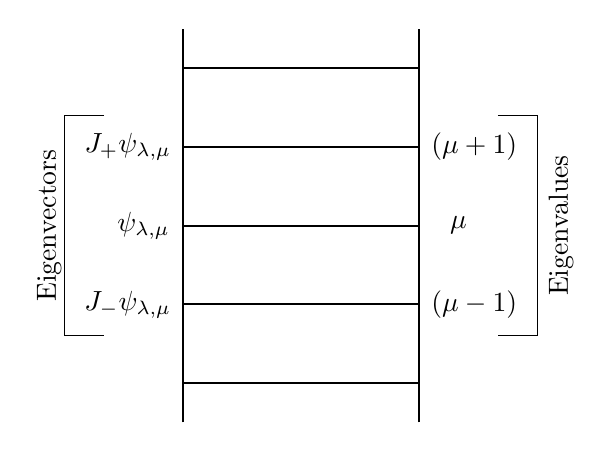
\begin{tikzpicture}
        \draw[thick] (0,0) -- (0,5); 
        \draw[thick] (3,0) -- (3,5);
        \draw[thick] (0,0.5) -- (3,0.5);
        \draw[thick] (0,1.5) -- (3,1.5);
        \draw[thick] (0,2.5) -- (3,2.5);
        \draw[thick] (0,3.5) -- (3,3.5);
        \draw[thick] (0,4.5) -- (3,4.5);
        %%%% 
        \node at (-0.5,2.5) {$\psi_{\lambda,\mu}$};
        \node at (-0.7,3.5) {$J_+\psi_{\lambda,\mu}$};
        \node at (-0.7,1.5) {$J_-\psi_{\lambda,\mu}$};
        \draw (-1, 3.9) -- (-1.5,3.9) -- (-1.5,1.1) -- (-1,1.1);
        \node[rotate = 90] at (-1.7,2.5) {Eigenvectors};
        \draw (4, 3.9) -- (4.5,3.9) -- (4.5,1.1) -- (4,1.1);
        \node[rotate = 90] at (4.8,2.5) {Eigenvalues};
        %%%%
        \node at (3.5,2.5) {$\mu$};
        \node at (3.7,3.5) {$(\mu+1)$};
        \node at (3.7,1.5) {$(\mu-1)$};
    \end{tikzpicture}
\end{center}
The next question would be is this a `proper' ladder; that is does it have a top and bottom rung or does it continue forever? The answer comes in the form of the next lemma. 
\er 

\bl 
There exists a $\psi_{\lambda,\overline{\mu}}$ such that $J_+\psi_{\lambda,\overline{\mu}} = 0$. Equally there exists a $\psi_{\lambda,\underline{\mu}}$ such that $J_-\psi_{\lambda,\underline{\mu}}=0$.  
\el 

\bq 
We know from \Cref{lem:CommonEigenvalueInequality} that $|\mu|(|\mu|+1) \leq \lambda$ holds for \emph{any} common eigenvector of $\Omega$ and $J_3$. We see from \Cref{lem:LadderEigenvalues} that $(J_{\pm})^n\psi_{\lambda,\mu}$ is such a common eigenvector, and so must obey $|\mu\pm n|(|\mu \pm n| +1)\leq \lambda$. However, $\lambda$ is unchanged by this repeated application of the ladder operators, and so, unless remedied,  this inequality will eventually be broken -- that is we need to somehow cap the available $n$ values. 

Consider first the raising operator. In this case $\mu+n$ gets bigger and bigger, and so we need to cap $n$ from above. In other words, we require there to be an $m\in\N$ such that for all $n > m$, $(J_+)^n\psi_{\lambda,\mu} = 0$. This fixes our problem as this corresponds to the zero vector and so, by definition, it cannot be a eigenvector, and the $\lambda$ inequality no longer need hold. We define 
\bse 
\psi_{\lambda,\overline{\mu}} := (J_+)^m\psi_{\lambda,\mu}.
\ese 

The idea is exactly the same is true for the lowering operator, however now $\mu-n$ is getting smaller and smaller, and so its modulus (after $n>\mu$ is reached) gets bigger and bigger. So again we need to cap $n$ from above. We require there to be a $\ell\in\N$ such that for all $n>\ell$, $(J_-)^n\psi_{\lambda,\mu}=0$. We define 
\bse 
\psi_{\lambda,\underline{\mu}} := (J_-)^{\ell} \psi_{\lambda,\mu}.
\ese 

Note we do not have any a priori relation between the values of $m$ and $\ell$. To use the ladder analogy, $m$ is the number of rungs above $\mu$-th rung and $\ell$ is the number of rungs below the $\mu$-th rung. For a given $\lambda$, the highest value of $\mu$ is denoted $\overline{\mu}(\lambda)$ and the lowest value $\underline{\mu}(\lambda)$. 
\eq 

\br 
Note the above tells us that $J_{\pm}\psi$ are not strictly eigenvalues, as it could be the zero vector. This is why we wrote `eigenvectors' in inverted commas in \Cref{lem:LadderEigenvalues}.
\er 

\bp 
The maximum and minimum values of $\mu$ satisfy 
\ben[label=(\roman*)]
\item $\lambda = \overline{\mu}(\lambda)\big(\overline{\mu}(\lambda)+1\big)$,
\item $\underline{\mu}(\lambda) = - \overline{\mu}(\lambda)$,
\item $\overline{\mu}(\lambda)\in\frac{\N_0}{2}$.
\een 
\ep 

\bq 
\ben[label=(\roman*)]
\item From the proof of \Cref{lem:CommonEigenvalueInequality}, and the fact that $J_+\psi_{\lambda,\overline{\mu}(\lambda)} = 0$, and so $\|J_+\psi_{\lambda,\overline{\mu}(\lambda)}\| = 0$, we have 
\bse
\lambda = \overline{\mu}(\lambda)\big(\overline{\mu}(\lambda)+1\big)
\ese
\item Repeating the above argument but with the fact that $\|J_-\psi_{\lambda,\underline{\mu}(\lambda)}\| = 0$, we have 
\bi{rCl}
\lambda & = & \underline{\mu}(\lambda)\big(\underline{\mu}(\lambda)-1\big) \\
& = & -\underline{\mu}(\lambda)\big(-\underline{\mu}(\lambda)+1\big),
\ei
and so $\underline{\mu}(\lambda) = -\overline{\mu}$.
\item From the previous, along with the fact that $\overline{\mu}(\lambda)-\underline{\mu}(\lambda) \in \N_0$ this result follows trivially.
\een 
\eq 

\br 
In order to be consistent with the literature we shall introduce the following relabelling 
\bse 
j := \overline{\mu}(\lambda), \qquad \qquad m := \mu.
\ese 
Note we have $j\in\frac{\N_0}{2}$.
\er 

\bt 
The \emph{common eigenvectors} of $\Omega$ and $J_3$ come as families $\psi_{j(j+1),m}$, where $m= -j,-j+1,...,j-1,j$. The eigenvalue $j(j+1)$ is associated to $\Omega$ and $m$ is associated to $J_3$.
\et 

One normally normalises these eigenvectors and defines 
\bse
\Phi_{j,m} := \frac{\psi_{j(j+1),m}}{\|\psi_{j(j+1),m}\|}.
\ese 
Then, from \Cref{lem:EigenvectorsOrthogonalDistinctEigenvalues} and the fact that the eigenvectors have distinct eigenvalues, we have 
\bse 
\braket{\Phi_{j,m}}{\Phi_{k,n}} = \delta_{jk}\delta_{mn}.
\ese 

\bc 
We have $m\in\frac{\Z}{2}$.
\ec 

\bq 
This comes from just allowing $j\in\frac{\N_0}{2}$ to be any element and then using $m=-j,...,j$. 
\eq 

\bp 
\label{prp:LadderCoefficients}
The the common eigenvectors $\Phi_{j,m}$ satisfy
\bi{rCl}
J_{\pm}\Phi_{j,m} = \sqrt{j(j+1) - m(m\pm1)}\Phi_{j,m\pm 1}.
\ei 
\ep 

\bq 
We shall show this for $J_+$, the method of $J_-$ follows analogously. Recall from \Cref{lem:CasimirLadder} that 
\bse  
J_-J_+ = \Omega - J_3(J_3+\id_{\cD}).
\ese
Now consider 
\bi{rCl}
\braket{J_+\Phi_{j,m}}{J_+\Phi_{j,m}} & = & \braket{\Phi_{j,m}}{J_-J_+\Phi_{j,m}} \\
& = & \braket{\Phi_{j,m}}{\Omega\Phi_{j,m}}  - \braket{\Phi_{j,m}}{J_3(J_3+\id_{\cD})\Phi_{j,m}} \\
& = & j(j+1) \braket{\Phi_{j,m}}{\Phi_{j,m}} - m(m+1)\braket{\Phi_{j,m}}{\Phi_{j,m}} \\
& = & j(j+1)-m(m+1).
\ei 
Combining this with \Cref{rem:LadderProportional} allows us to conclude the result. 
\eq 

\subsection{Pure Spin-$j$ Systems}

\bd 
A quantum mechanical system is called a \emph{pure spin-$j$} system if its Hilbert space is $(2j+1)$-dimensional that possesses an orthonormal eigenbasis $\{\Phi_{j,m}\}$ for the three operators $J_1,J_2,J_3$ defined on $\cH$.
\ed 

\bc 
The Hilbert space is isomorphic to $\C^{2j+1}$.
\ec 

\bc 
For a pure spin-$j$ system the spectrum of the operators is 
\bse
\sigma(J_i) = \{-j,-j+1,...,j-1,j\},
\ese 
for $i=1,2,3$.
\ec 

\be 
\hfill 

\begin{center}
    \begin{tabular}{c|c}
        $j$ & $\sigma(J_i)$, $i=1,2,3$ \\
         \hline $0$ & $0$ \\
         $1/2$ & $\{-1/2,1/2\}$ \\
         $1$ & $\{-1,0,1\}$
    \end{tabular}
\end{center}
\ee 

\br 
\label{rem:ElectronCompositeHilbert}
When you introduce spin to a particle, its Hilbert space becomes a product space. For example for an electron (spin-$1/2$) in $\R^3$ its Hilbert space is 
\bse
\cH_{e} = L^2(\R^3)\otimes \C^2.
\ese 
We shall return to this and expand on it in the next lecture.
\er 

\br 
You can also have non-pure spin systems. For the orbital angular momentum, you take a direct sum of the Hilbert spaces. That is if $\cH_j$ is the Hilbert space associated to the pure spin-$j$ system then the composite system's Hilbert space is 
\bse 
\cH_{comp} = \bigoplus_{j}\cH_j.
\ese 
We shall return to this in two lectures time.
\er 
\newpage

\section{Composite Systems}
Recall Axiom 1, which says that to every quantum system there is an underlying Hilbert space. The question we now want to ask is: Let $\cH_1$ be the Hilbert space associated to one system and $\cH_2$ be the Hilbert space associated to another. What is the underlying Hilbert space associated to the composite system? 

To clarify what we mean, imagine having a proton and an electron. We first look at the proton by itself and call this system one. We then look at the electron separately and call that system two. We now want to look at both of them together, but we wish to use the fact that we have already studied them separately to simplify the problem. It may seem `natural' to model the composite $\cH$ as the so called \emph{direct sum}, which as a set is\footnote{This definition holds as we are only taking the direct product of two spaces, and so the index set is finite. See \href{https://en.wikipedia.org/wiki/Direct_sum}{wiki} for details on this.}
\bse 
\cH_1\oplus \cH_2 := \{ (\psi,\varphi) \, | \, \psi\in\cH_1, \varphi\in\cH_2 \},
\ese 
and where the linearity is inherited from $\cH_1$ and $\cH_2$, namely  
\bse 
(a\psi_1+\psi_2,b\varphi_1+\varphi_2) = ab(\psi_1,\varphi_1) + a(\psi_1,\varphi_2) + b(\psi_2,\varphi_1) + (\psi_2,\varphi_2).
\ese 
This is what we do in classical systems and it tells us that if we know everything about the states\footnote{Recall that the elements of the Hilbert space are \emph{not} the states, but are associated to them. We shall return to this at the end of the lecture.} of our two systems, then we also know everything about the states of the composite system. 

However, as with all things quantum, things are more complicated, and the above is not the case. The main problem comes from the fact that not all linear combinations of elements of the form $(\psi,\varphi)$ can also be written in that form. 

\be 
Let $\psi_1,\psi_2\in\cH_1$, $\varphi_1,\varphi_2\in\cH_2$ and $a,b\in\C$. Then, assuming the linearity as above, we have 
\bi{rCl}
a(\psi_1,\varphi_1)+b(\psi_2,\varphi_2) & = & (a\psi_1,\varphi_1)+(\psi_2,b\varphi_2) \\
& = & (a\psi_1 + \psi_2,\varphi_1+b\varphi_2) \\
& = & a(\psi_1,\varphi_1)+b(\psi_2,\varphi_2)+ab(\psi_1,\varphi_2) + (\psi_2,\varphi_1),
\ei 
a clear problem.
\ee
Note this example actually tells us that we $\cH_1\oplus\cH_2$ is not closed under the linearity, and so would not be a vector space. We could just restrict ourselves to elements that do obey these rules, however, as we shall see when considering entanglement, we require elements of this form in our underlying Hilbert space.  

This calls for a slight refinement of axiom one. We add the addendum\footnote{We shall define what these new terms are in the next section.}: 

\begin{tcolorbox}[colframe=blue!10!black,before skip=10pt,after skip=10pt]
If a quantum system is composed of two (and hence, by induction, any finite number) of `sub'systems, then its underlying Hilbert space is the \emph{tensor product space} $\cH_1\otimes\cH_2$, equipped with a inner product.
\end{tcolorbox}

\be 
\Cref{rem:ElectronCompositeHilbert} is an example of such a composite system.
\ee 

\subsection{Tensor Product of Hilbert Spaces}

In order to give a nice definition for the tensor product of two vector spaces, we first need to introduce the so called \emph{free vector space}.

\bd 
Let $V$ be a $\F$-vector space and let $B\se V$ be a generating subset of $V$ (i.e. any element of $V$ can be obtained via finite linear combinations of elements of $B$). The the \emph{free vector space} is 
\bse 
F(B) := \text{span}_{\F}(B),
\ese 
i.e. the set of all linear combinations of elements of $B$.
\ed 

\bl 
Every vector space is a free vector space with $B$ being a Hamel basis.
\el 

\br 
\label{rem:F(B)notV}
Note it need not be true that $F(B)=V$, as it might be the case that the same element in $V$ is reached via two different linear combinations of elements of $B$. In fact if $F(B)=V$, then $B$ is just a Hamel basis.
\er 

The free vector space for vector spaces might seem almost redundant, given that every vector space has a basis. However if your vector space is countably infinite then such a basis might be incredibly difficult to construct. However you can simply take the entire set for $B$ and construct the free vector space $F(V)$, which will be a huge set, mind. Note, then, that any linear combination of elements in this set is automatically still in the set, and so it is indeed a vector space.

\bd 
Let $V$ and $W$ be two $\F$-vector spaces, and let $A\se V$ and $B\se W$ be generating subsets. Then we define their tensor product as the vector space with set 
\bse 
V\otimes W := F(A\times B)/_{\sim},
\ese 
where $\times$ is the Cartesian prodcut and $\sim$ is an equivalence relation such that: if $a,a_1,a_2\in A$, $b,b_1,b_2\in B$ and $f\in\F$ then 
\ben[label=(\roman*)]
\item $(a,b)\sim(a,b)$, 
\item $(a_1,b_1) + (a_1,b_2) \sim (a_1,b_1+b_2)$ and $(a_1,b_1) + (a_2,b_1) \sim (a_1+a_2,b_1)$, and continued by induction,
\item $f(a,b) \sim (fa,b)$ and $f(a,b)\sim(a,fb)$. 
\item Combinations of (ii) and (iii), e.g. $(a_1,b_1)+f(a_1,b_2) \sim (a_1,b_1+fb_2)$. 
\een 
\ed 

\br 
Note the equivalence relation looks a lot like a linearity condition on $V\otimes W$, however on closer inspection it is not quite. The linearity condition that make $V\otimes W$ into a vector space is simply 
\bse 
f(a_1,b_1) + (a_2,b_2) \in V\otimes W.
\ese 
This, in itself, does not need to satisfy the equivalence relation. However, if we did not include it we could end up with a huge redundancy in elements, as a repercussion of \Cref{rem:F(B)notV}. This equivalence relation makes the corresponding set of equivalence classes a vector space in the way we normally think of them (there is no repeated elements).
\er 

This is exactly the type of structure we need to overcome the problem highlighted before (that not all linear combinations can be expressed as a single term), as now we only require that linear combinations of linear combinations are linear combinations, which they obviously are.

\bp 
\label{prp:EquivAdditionH12}
Let $\cH_1$ and $\cH_2$ be our two vector spaces. We can define the map 
\bi{rrCl}
+_{\cH_1\otimes\cH_2} \cl & (\cH_1\otimes\cH_2)\times (\cH_1\otimes\cH_2) & \to & (\cH_1\otimes\cH_2) \\
& \big([(\psi,\varphi_1)],[(\psi,\varphi_2)]\big) & \mapsto & [(\psi,\varphi_1)]+_{\cH_1\otimes\cH_2} [(\psi,\varphi_2)] := [(\psi,\varphi_1)+(\psi,\varphi_2)],
\ei 
where the additions inside the brackets are w.r.t. $\cH_1$ and $\cH_2$. 
\ep 

\bq 
We need to show this is well defined. We shall write $+_{12}$ now in order to lighten notation. Consider it case by case. 
\ben[label=(\roman*)]
\item Assume $(\widetilde{\psi},\widetilde{\varphi_1})= (\psi,\varphi_1)$. 
\ben 
\item If $(\widetilde{\psi},\widetilde{\varphi_2})= (\psi,\varphi_2)$, then it follows trivially that 
\bse 
[(\widetilde{\psi},\widetilde{\varphi_1})+(\widetilde{\psi},\widetilde{\varphi_2})] = [(\psi,\varphi_1)+(\psi,\varphi_2)],
\ese 
and so 
\bse 
[(\widetilde{\psi},\widetilde{\varphi_1})] +_{12} [(\widetilde{\psi},\widetilde{\varphi_2})] = [(\psi,\varphi_1)] +_{12} [(\psi,\varphi_2)].
\ese 
\item If $(\widetilde{\psi},\widetilde{\varphi_2})= (\psi,\varphi_2^1)+(\psi,\varphi_2^2)$, where $\varphi_2=\varphi_2^1+\varphi_2^2$, we have 
\bi{rCl}
[(\widetilde{\psi},\widetilde{\varphi_1})+(\widetilde{\psi},\widetilde{\varphi_2})] & = & [(\psi,\varphi_1)+(\psi,\varphi_2^1)+(\psi,\varphi_2^2)] \\
& = & [(\psi,\varphi_1+\varphi_2^1+\varphi_2^2)] \\
& = & [(\psi,\varphi_1+\varphi_2)] \\
& = & [(\psi,\varphi_1)+(\psi,\varphi_2)],
\ei 
and so 
\bse 
[(\widetilde{\psi},\widetilde{\varphi_1})] +_{12} [(\widetilde{\psi},\widetilde{\varphi_2})] = [(\psi,\varphi_1)] +_{12} [(\psi,\varphi_2)].
\ese 
\item If $(\widetilde{\psi},\widetilde{\varphi_2}) = f(\psi,\varphi_2^3)$, where $\varphi_2=f\varphi_2^3$, then
\bi{rCl}
[(\widetilde{\psi},\widetilde{\varphi_1})+(\widetilde{\psi},\widetilde{\varphi_2})] & = & [(\psi,\varphi_1)+f(\psi,\varphi_2^3)] \\
& = & [(\psi,\varphi_1)+(\psi,f\varphi_2^3)] \\
& = & [(\psi,\varphi_1)+(\psi,\varphi_2)],
\ei 
and so 
\bse 
[(\widetilde{\psi},\widetilde{\varphi_1})] +_{12} [(\widetilde{\psi},\widetilde{\varphi_2})] = [(\psi,\varphi_1)] +_{12} [(\psi,\varphi_2)].
\ese 
\een 
\item Assume $(\widetilde{\psi},\widetilde{\varphi_1})=(\psi,\varphi_1^1) +(\psi,\varphi_1^2)$ where $\varphi_1=\varphi_1^1+\varphi_1^2$.
\ben 
\item If $(\widetilde{\psi},\widetilde{\varphi_2})=(\psi,\varphi_2)$ then we have essentially the same as (i)(b), so we wont re-write it here. 
\item If $(\widetilde{\psi},\widetilde{\varphi_2})= (\psi,\varphi_2^1)+(\psi,\varphi_2^2)$, where $\varphi_2=\varphi_2^1+\varphi_2^2$, we have
\bi{rCl}
[(\widetilde{\psi},\widetilde{\varphi_1})+(\widetilde{\psi},\widetilde{\varphi_2})] & = & [(\psi,\varphi_1^1)+(\psi,\varphi_1^2)+(\psi,\varphi_2^1)+(\psi,\varphi_2^2)] \\
& = & [(\psi,\varphi_1^1+\varphi_1^2+\varphi_2^1+\varphi_2^2)] \\
& = & [(\psi,\varphi_1+\varphi_2)] \\
& = & [(\psi,\varphi_1)+(\psi+\varphi_2)],
\ei 
and so 
\bse 
[(\widetilde{\psi},\widetilde{\varphi_1})] +_{12} [(\widetilde{\psi},\widetilde{\varphi_2})] = [(\psi,\varphi_1)] +_{12} [(\psi,\varphi_2)].
\ese 
\item If $(\widetilde{\psi},\widetilde{\varphi_2})=f(\psi,\varphi_2^3)$ where $\varphi_2=f\varphi_2^3$, then we have 
\bi{rCl}
[(\widetilde{\psi},\widetilde{\varphi_1})+(\widetilde{\psi},\widetilde{\varphi_2})] & = & [(\psi,\varphi_1^1)+(\psi,\varphi_1^2)+f(\psi,\varphi_2^3)] \\
& = & [(\psi,\varphi_1^1+\varphi_1^2+f\varphi_2^3)] \\
& = & [(\psi,\varphi_1+\varphi_2)] \\
& = & [(\psi,\varphi_1)+(\psi,\varphi_2)]
\ei 
and so 
\bse 
[(\widetilde{\psi},\widetilde{\varphi_1})] +_{12} [(\widetilde{\psi},\widetilde{\varphi_2})] = [(\psi,\varphi_1)] +_{12} [(\psi,\varphi_2)].
\ese 
\een 
\item Assume $(\widetilde{\psi},\widetilde{\psi_1})\sim g(\psi,\varphi_1^3)$, where $\varphi_1=g\varphi_1^3$. 
\ben 
\item If $(\widetilde{\psi},\widetilde{\varphi_2})=(\psi,\varphi_2)$, then we have basically same as (i)(c) and so we wont write it again. 
\item If $(\widetilde{\psi},\widetilde{\varphi_2})=(\psi,\varphi_2^1)+(\psi,\varphi_2^2)$, where $\varphi_2=\varphi_2^1+\varphi_2^2$, then we are basically the same as (ii)(c) and so we wont write it again.
\item If $(\widetilde{\psi},\widetilde{\varphi_2})=f(\psi,\varphi_2^3)$, where $\varphi_2=f\varphi_2^3$ then 
\bi{rCl}
[(\widetilde{\psi},\widetilde{\varphi_1})+(\widetilde{\psi},\widetilde{\varphi_2})] & = & [g(\psi,\varphi_1^3)+f(\psi,\varphi_2^3)] \\
& = & [(\psi,g\varphi_1^3+f\varphi_2^3)] \\
& = & [(\psi,\varphi_1+\varphi_2] \\
& = & [(\psi,\varphi_1)+(\psi,\varphi_2)]
\ei 
and so 
\bse 
[(\widetilde{\psi},\widetilde{\varphi_1})] +_{12} [(\widetilde{\psi},\widetilde{\varphi_2})] = [(\psi,\varphi_1)] +_{12} [(\psi,\varphi_2)].
\ese 
\een 
\een 
\eq 

\br 
We can do exactly the same thing but for a map that has the first element different and the second element the same. 
\er 

\bd 
Let $\cH_1$ and $\cH_2$ be complex Hilbert spaces with sesqui-linear inner products $\braket{\cdot}{\cdot}_{\cH_1}$ and $\braket{\cdot}{\cdot}_{\cH_2}$, respectively. Then the \emph{composite Hilbert space} is the Hilbert space with set 
\bse 
\cH_1\otimes \cH_2 := \overline{F(\cH_1\times\cH_2)/_{\sim}},
\ese 
where the overline indicates the topological closure, and with sesqui-linear inner product: for $\psi_1,\psi_2\in\cH_1$ and $\varphi_1,\varphi_2\in\cH_2$,
\bse 
\braket{[(\psi_1,\varphi_1)]}{[(\psi_2,\varphi_2)]}_{\cH_1\otimes\cH_2} := \braket{\psi_1}{\psi_2}_{\cH_1} \cdot  \braket{\varphi_1}{\varphi_2}_{\cH_2},
\ese 
extended by linearity, with respect to which the closure is taken (i.e. the topology is derived from here).
\ed 

\br 
Note, we need to take the topological closure as the free vector space only considers \emph{finite} linear combinations, but our Hilbert spaces could be infinite dimensional.
\er 

\bq 
(that we have a sesqui-linear inner product). 
\ben[label=(\roman*)]
\item Conjugate symmetry. 
\bi{rCl}
\overline{\braket{[(\psi_1,\varphi_1)]}{[(\psi_2,\varphi_2)]}_{\cH_1\otimes\cH_2}} & = & \overline{\braket{\psi_1}{\psi_2}_{\cH_1}} \cdot \overline{\braket{\varphi_1}{\varphi_2}_{\cH_2}} \\
& = & \braket{\psi_2}{\psi_1}_{\cH_1}\cdot \braket{\varphi_2}{\varphi_1}_{\cH_2} \\
& =: & \braket{[(\psi_2,\varphi_2)]}{[(\psi_1,\varphi_1)]}_{\cH_1\otimes\cH_2}
\ei 
\item Linearity in second argument. The extension by linearity means
\bi{rCl}
\braket{[(\psi_1,\varphi_1)]}{\sum_iz_i[(\psi_i,\varphi_i)}_{\cH_1\otimes\cH_2} & := & \sum_iz_i \braket{\psi_1}{\psi_i}_{\cH_1} \cdot  \braket{\varphi_1}{\varphi_i}_{\cH_2} \\
& = & \sum_iz_i\braket{[(\psi_1,\varphi_1)]}{[(\psi_i,\varphi_i)]}_{\cH_1\otimes\cH_2},
\ei 
for $z_i\in\C$.
\item Positive-definiteness. As $\braket{\cdot}{\cdot}_{\cH_1},\braket{\cdot}{\cdot}_{\cH_1}\geq 0$ it follows that\footnote{We shall use $`-'$ for empty slots on the composite space.} $\braket{-}{-}_{\cH_1\otimes\cH_2}\geq 0$. Then from 
\bse 
(0_{\cH_1},\varphi) = (0\cdot \psi, \varphi) \sim  0(\psi,\varphi) \sim  (\psi,0\cdot\varphi) = (\psi,0_{\cH_2}),
\ese 
we have 
\bse 
[(0_{\cH_1},\varphi)] = [(\psi,0_{\cH_2})] =: 0_{\cH_1\otimes\cH_2}.
\ese 
Finally, from
\bi{rCl}
0 & = & \braket{[(\psi,\varphi)]}{[(\psi,\varphi)]}_{\cH_1\otimes\cH_2} \\
& := & \braket{\psi}{\psi}_{\cH_1}\cdot\braket{\varphi}{\varphi}_{\cH_2},
\ei 
which implies either $\psi=0_{\cH_1}$ and/or $\varphi=0_{\cH_2}$, and so $[\psi,\varphi]=0_{\cH_1\otimes\cH_2}$.
\een 
\eq


We also need to check that the sesqui-linear inner product is well defined. 

\bq 
The proof follows a similar method to the proof of \Cref{prp:EquivAdditionH12}. We shall just show the first two results here in order to save space. 
\ben[label=(\roman*)]
\item Assume $(\widetilde{\psi_1},\widetilde{\varphi_1}) = (\psi_1,\varphi_1)$. 
\ben
\item If $(\widetilde{\psi_2},\widetilde{\varphi_2}) = (\psi_2,\varphi_2)$. The inner product result follows trivially. 
\item $(\widetilde{\psi_2},\widetilde{\varphi_2}) = (\psi_2,\varphi_2^3)+(\psi_2,\varphi_2^4)$, where $\varphi_2=\varphi_3+\varphi_4$, 
\bi{rCl}
\braket{[(\widetilde{\psi_1},\widetilde{\varphi_1})]}{[\widetilde{\psi_2},\widetilde{\varphi_2})]}_{12} & = &  \braket{[(\psi_1,\varphi_1)]}{[(\psi_2,\varphi_2^3)+(\psi_2,\varphi_2^4)]}_{12} \\
& = & \braket{[(\psi_1,\varphi_1)]}{[(\psi_2,\varphi_2^3)]+_{12}[(\psi_2,\varphi_2^4)]}_{12} \\
& = & \braket{[(\psi_1,\varphi_1)]}{[(\psi_2,\varphi_2^3)]}_{12} + \braket{[(\psi_1,\varphi_1)]}{[(\psi_2,\varphi_2^4)]}_{12} \\
& := & \braket{\psi_1}{\psi_2}_1 \braket{\varphi_1}{\varphi_2^3}_2 + \braket{\psi_1}{\psi_2}_1 \braket{\varphi_1}{\varphi_2^4}_2 \\
& = & \braket{\psi_1}{\psi_2}_1 \cdot \Big( \braket{\varphi_1}{\varphi_2^3}_2 + \braket{\varphi_1}{\varphi_2^4}_2 \Big) \\
& = & \braket{\psi_1}{\psi_2}_1 \braket{\varphi_1}{\varphi_2^3+\varphi_2^4}_2 \\
& = & \braket{\psi_1}{\psi_2}_1 \braket{\varphi_1}{\varphi_2}_2 \\
& =: & \braket{[(\psi_1,\varphi_1)]}{[(\psi_2,\varphi_2)]}_{12}.
\ei 
\een 
\een 
\eq 

We introduce the new notation 
\bse 
\psi\boxtimes\varphi := [(\psi,\varphi)].
\ese 
Here we have used a $\boxtimes$ for the tensor product of two vectors. We have done this in order to highlight the fact that it is \emph{not} the same thing as $\otimes$, which is the tensor product between vector spaces. We will, however, end up using $\otimes$ for \emph{all} tensor products later, as this is the common notation. It is important to remember that they are distinctly different objects, and, if in doubt, we should go back to the definitions to clarify the circumstance. 

In this new notation we can rewrite the definition for the sesqui-linear inner product simply as 
\bse 
\braket{\psi\boxtimes\varphi}{\widetilde{\psi}\boxtimes\widetilde{\varphi}}_{\cH_1\times\cH_2} := \braket{\psi}{\widetilde{\psi}}_{\cH_1}\braket{\varphi}{\widetilde{\varphi}}_{\cH_2},
\ese 
extended by linearity. 

\be 
This example acts as a further warning that its important that we consider the space $F(\cH_1\times\cH_2)$ and not just $\cH_1\times\cH_2$. 

Let $\cH_1=\cH_2=\C^2$. Then we can express the elements at 2x1 matrices, in which case we can consider $\boxtimes$ to be the outer product. Note then that 
\bse 
\begin{pmatrix}
1 \\
0 
\end{pmatrix} \boxtimes \begin{pmatrix}
0 \\
1 
\end{pmatrix} - \begin{pmatrix}
0 \\
1
\end{pmatrix} \boxtimes \begin{pmatrix}
1 \\ 
0 
\end{pmatrix} = \begin{pmatrix}
0 & 1 \\
0 & 0 
\end{pmatrix} - \begin{pmatrix}
0 & 0 \\
1 & 0 
\end{pmatrix} = \begin{pmatrix}
0 & 1 \\
-1 & 0 
\end{pmatrix}
\ese 
is in $\cH_1\otimes\cH_2$, but it \emph{cannot} be written as $\psi\boxtimes\varphi$ for some $\psi\in\cH_1$ and $\varphi\in\cH_2$.
\ee 

\bt 
Let $\{e_i\}_{i=1,...,\dim(\cH_1)}$ and $\{f_i\}_{i=1,...,\dim(\cH_2)}$ be a Schauder (ON)-bases for $\cH_1$ and $\cH_2$ respectively. Then we can construct a Schauder (ON)-basis for $\cH_1\otimes\cH_2$ as 
\bse 
\{e_i\boxtimes f_j\}_{\substack{i=1,...,\dim(\cH_2) \\ j=1,...,\dim(\cH_2)}}
\ese 
\et 

\bc 
We can rewrite 
\bse 
\cH_1\otimes\cH_2 := \bigg\{\sum_{i=1}^{\dim(\cH_1)} \sum_{j=1}^{\dim(\cH_2)} a_{ij} e_i\boxtimes f_j \,  \Big| \, a_{ij}\in\C, \sum_{i,j} |a_{ij}|^2 <\infty \bigg\},
\ese 
from which it also follows that 
\bse 
\dim(\cH_1\otimes\cH_2) = \dim(\cH_1)\cdot\dim(\cH_2).
\ese 
\ec 

\subsection{Practical Rules for Tensor Products of Vectors} 

This short section just highlights a couple rules obeyed by $\boxtimes$. 
\ben[label=(\roman*)]
\item Let $\psi_1,\psi_2\in\cH_1$, $\varphi_1,\varphi_2\in\cH_2$ and $\alpha,\beta\in\C$. Then the following holds 
\bse 
(\psi_1+\alpha\psi_2)\boxtimes(\varphi_1+\beta\varphi_2) = \psi_1\boxtimes\varphi_1 + \alpha\psi_2\boxtimes\varphi_1 + \beta\psi_1\boxtimes\varphi_2 + \alpha\beta\psi_2\varphi_2.
\ese 
\item Given that $\{e_i\boxtimes f_j\}$ is a basis, we have: 
\bse 
\forall \Psi\in\cH_1\otimes\cH_2 \quad  \exists a_{ij}\in\C \, : \, \Psi := \sum_{i,j}a_{ij} e_i\boxtimes f_j.
\ese 
\een 

\br 
\label{rmk:TensorOrderMatters}
Note, obviously, that the order matters when taking a tensor product. In other words, in general 
\bse 
\psi\boxtimes\varphi \neq \varphi\boxtimes\psi. 
\ese 
Note, its not even a case of `choosing the right $\psi$ and $\varphi$', as the LHS is an element of $\cH_1\otimes\cH_2$ whereas the RHS is an element of $\cH_2\otimes \cH_1$. So, unless the two spaces are the same, they could never be equal. 
\er 

\subsection{Tensor Product Between Operators}

\bd 
Let $A:\cH_1\to\cH_1$ and $B:\cH_2\to\cH_2$ be linear maps. Then we define their tensor product as 
\bi{rrCl}
A\widehat{\otimes} B \, : \, & \cH_1\otimes\cH_1 & \to & \cH_1\otimes\cH_2 \\
& \psi\boxtimes\varphi & \mapsto & (A\widehat{\otimes} B)(\psi\boxtimes\varphi) := (A\psi)\boxtimes(B\varphi).
\ei 
\ed 

\bt 
If $A:\cH_1\to\cH_1$ and $B:\cH_2\to\cH_2$ are self adjoint then their tensor product $A\widehat{\otimes} B$ is also self adjoint on $\cH_1\otimes\cH_2$.
\et 

\bq 
We have $A=A^*$ and $B=B^*$, i.e. that their domains coincide and $A\psi=A^*\psi$ for all $\psi\in\cD_A$ and similarly for $B$ and $B^*$. Then we have 
\bi{rrCl}
A\widehat{\otimes} B \, : \, & \cD_A\otimes\cD_B & \to & \cH_1\otimes\cH_2 \\
& \psi\boxtimes\varphi & \mapsto &  (A\psi)\boxtimes(B\varphi),
\ei 
and 
\bi{rrCl}
A^*\widehat{\otimes} B^* \, : \, & \cD_A\otimes\cD_B & \to & \cH_1\otimes\cH_2 \\
& \psi\boxtimes\varphi & \mapsto &  (A^*\psi)\boxtimes(B^*\varphi) = (A\psi)\boxtimes(B\varphi),
\ei 
and so the domain concides and they have the same result for all $\psi\boxtimes\varphi\in\cD_A\otimes\cD_B$. So it is self adjoint.
\eq 

\bt 
\label{thrm:SigmaTensorProduct}
If $A:\cH_1\to\cH_1$ and $B:\cH_2\to\cH_2$ are self adjoint then
\ben[label=(\roman*)]
\item $\sigma(A\widehat{\otimes} B) = \overline{\sigma(A)\cdot\sigma(B)}$, where the overline is the topological closure and the $\cdot$ indicates all possible products of elements in the sets. 
\item $\sigma(A\widehat{\otimes}\id_{\cH_2} + \id_{\cH_1}\widehat{\otimes} B) = \overline{\sigma(A)+\sigma(B)}$, where again the overline is the topological closure.
\een
\et 

An application of the second of these results finds use when you know how to measure the observable $A$ on system 1 and $B$ on system 2, then you can measure them on the composite system. 

\subsection{Symmetric and Antisymmetric Tensor Products}

Recalling \Cref{rmk:TensorOrderMatters}, if we do have $\cH_1=\cH_2$ it is possible to define a symmetric and a antisymmetric tensor product. These definitions are important in quantum mechanics as they allow us to categorise particles according to their so called \emph{exchange statistics}. The symmetric composite system concerns a system of two (and by induction, any number) of \emph{bosons}, whereas the antisymmetric one corresponds to \emph{fermions}. These are both examples of what are known as \emph{indistinguishable particles}, meaning that two fermions of the same type (two electrons, say) cannot be distinguished from each other. 
A good analogy is to consider two identical looking balls. Imagine being in a room with the two balls on the floor. Someone asks you to leave the room and then calls you back in. They then ask you whether the two balls, still in the same places on the floor, have switched places or not? Of course there is no way for you to know, as they look identical, and you weren't present when they potentially could have switched. 

The version in QM is related to whether they live on the same Hilbert space. Recalling \Cref{rem:ElectronCompositeHilbert}, we see that this means that, not only are they allowed to move within the same physical space, they also have the same angular momentum (or \emph{spin}). For the two particles to be indistinguishable, their composite Hilbert spaces must be the same. For example, if a divider was put between the balls, and you knew the balls could only move along the floor, you would know that they couldn't possibly have changed places --- this could correspond to one electron having $L^2(U,\lambda)$ and the other having $L^2(V,\lambda)$ where $U,V\ss R^3$ with $U\cap V =\varnothing$.

\bd 
Let $\psi,\varphi\in\cH$, then we define their \emph{symmetric} tensor product as 
\bse 
\psi \boxdot \varphi := \frac{1}{2}(\psi\boxtimes\varphi + \varphi\boxtimes\psi),
\ese 
which is an element of the \emph{symmetric composite Hilbert space}, defined as 
\bse 
\cH\odot\cH := \Bigg\{ \sum_{i,j=1}^{\dim(\cH)}a_{ij}e_i\boxdot e_j \, \Big| \, a_{ij}\in\C, \sum_{i,j}|a_{ij}|^2<\infty\Bigg\},
\ese 
where $\{e_i\}$ is a basis of $\cH$.
\ed 

\br 
Note it follows from the definition that $a_{ij}=a_{ji}$ for a symmetric composite Hilber space. 
\er 

\bd 
Let $\psi,\varphi\in\cH$, then we define their \emph{antisymmetric} tensor product as 
\bse 
\psi \boxwedge \varphi := \frac{1}{2}(\psi\boxtimes\varphi - \varphi\boxtimes\psi),
\ese 
which is an element of the \emph{antisymmetric composite Hilbert space}, defined as 
\bse 
\cH\owedge\cH := \Bigg\{ \sum_{i,j=1}^{\dim(\cH)}a_{ij}e_i\boxwedge e_j \, \Big| \, a_{ij}\in\C, \sum_{i,j}|a_{ij}|^2<\infty\Bigg\}
\ese 
\ed 

\br 
Note it follows from the definition that $a_{ij}=-a_{ji}$ for a antisymmetric composite Hilber space. 
\er 

\br 
For $\psi\in\cH$ we have $\psi\boxwedge\psi = 0$, which is known as the \emph{Pauli exclusion principle for Fermions}.
\er 

\br 
For $\psi,\varphi\in\cH$ where $\psi$ and $\varphi$ are linearly independent, then 
\bse 
\psi\boxwedge\varphi = \frac{1}{2} (\psi\boxtimes\varphi - \varphi\boxtimes\psi) \neq \widetilde{\psi}\boxtimes\widetilde{\varphi},
\ese 
for some $\widetilde{\psi},\widetilde{\varphi}\in\cH$. Which again emphasises that its important we consider the space of all linear combinations. 
\er 

\bd 
Let $A,B:\cH\to\cH$ be linear operators. Then we can define the \emph{symmetric tensor product of linear maps} as 
\bi{rrCl}
A\widehat{\odot} B : & \cH\odot\cH & \to & \cH\odot\cH \\
& \psi\boxdot \varphi & \mapsto & (A\widehat{\odot} B)(\psi\boxdot \varphi) := (A\psi)\boxdot(B\varphi).
\ei 
\ed 

\bd 
Let $A,B:\cH\to\cH$ be linear operators. Then we can define the \emph{antisymmetric tensor product of linear maps} as 
\bi{rrCl}
A\widehat{\owedge} B : & \cH\owedge\cH & \to & \cH\owedge\cH \\
& \psi\boxwedge \varphi & \mapsto & (A\widehat{\owedge} B)(\psi\boxwedge \varphi) := (A\psi)\boxwedge(B\varphi).
\ei 
\ed 

\subsection{Collapse of Notation}

As mentioned before, we shall now change our notation to that of the standard literature. That is 
\bi{rCl}
\otimes, \boxtimes, \widehat{\otimes} & \to & \otimes, \\
\odot, \boxdot, \widehat{\odot} & \to & \odot, \\
\owedge, \boxwedge, \widehat{\owedge} & \to & \wedge.
\ei 

\subsection{Entanglement}

As has been stressed many times, recall 
\bse 
\{\psi\otimes\varphi \, | \, \psi\in\cH_1, \varphi\in\cH_2\} \subsetneqq \cH_1\otimes\cH_2.
\ese 

\bd 
We call an element $\Psi\in\cH_1\otimes\cH_2$ \emph{simple} if there exists a $\psi\in\cH_1$ and a $\varphi\in\cH_2$ such that 
\bse 
\Psi = \psi\otimes\varphi.
\ese 
If it is not of this form (i.e. you need linear combinations) then it is called \emph{non-simple}.
\ed 

Recall: A state $\rho:\cH\to\cH$ is called \emph{pure} if
\bse 
\exists \psi \in\cH \, : \, \forall \alpha\in\cH \, : \, \rho_{\psi}(\alpha) = \frac{\braket{\psi}{\varphi}}{\braket{\psi}{\psi}} \psi,
\ese 
or, equivalently, we can think of 
\bse 
\rho_{\psi}(\cdot) := \frac{\braket{\psi}{\cdot}}{\braket{\psi}{\psi}} \psi.
\ese 

\bd 
Let $\Psi\in\cH_1\otimes\cH_2$. Then a pure state $\rho_{\Psi}$ on the composite system is called \emph{non-entangled} if there exists $\rho_{\psi}$ and $\rho_{\varphi}$ for $\psi\in\cH_1$ and $\varphi\in\cH_2$ such that\footnote{Note the tensor product here is that between linear operators.} 
\bse 
\rho_{\Psi} = \rho_{\psi}\otimes\rho_{\varphi}.
\ese 
Otherwise, the state is called \emph{entangled}.
\ed 

\bl 
A state $\rho_{\Psi}$ is non-entangled if and only if $\Psi$ is simple.
\el 

\bq 
Assume $\Psi$ is simple. Then 
\bi{rCl}
\rho_{\Psi}(\cdot) & = & \frac{\braket{\Psi}{\cdot}_{12}}{\braket{\Psi}{\Psi}_{12}}\Psi \\
& = & \frac{\braket{\psi\otimes\varphi}{\cdot}_{12}}{\braket{\psi\otimes\varphi}{\psi\otimes\varphi}_{12}}\psi\otimes\varphi \\
& = & \frac{\braket{\psi}{\cdot}_1\braket{\varphi}{\cdot}_2}{\braket{\psi}{\psi}_1\braket{\varphi}{\varphi}_2}\psi\otimes\varphi \\
& = & \bigg(\frac{\braket{\psi}{\cdot}_1}{\braket{\psi}{\psi}_1}\psi\bigg)\otimes \bigg(\frac{\braket{\varphi}{\cdot}_2}{\braket{\varphi}{\varphi}_2}\varphi\bigg) \\
& = & (\rho_{\psi}(\cdot)\big)\otimes (\rho_{\varphi}(\cdot)\big),
\ei 
where in the last two lines the $\otimes$ is the tensor product between linear maps. 

The reverse part of the proof (starting from $\rho_{\Psi}$ non-entangled) follows from working backwards through the above. 
\eq 

\bl 
A state $\rho_{\Psi}$ is entangled if and only if $\Psi$ is non-simple. 
\el 

\bq 
This proof is trivial given the previous one, as if $\Psi$ is non-simple then $\rho_{\Psi}$ cannot be non-entangled, and vice versa. 
\eq 
\newpage

\section{Total Spin of Composite System}
The lecture aims to answer the following question: "What is the total angular momentum (or spin) of a bi-partite system if we know the spin of each constituent system?" 

More precisely, in the context of quantum mechanics, consider a spin-$j_A$ system with Hilbert space $\cH_A$ and angular momentum operators $A_1,A_2,A_3$ and a spin-$j_B$ system with Hilbert space $\cH_B$ and angular momentum operators $B_1,B_2,B_3$. Then what is the spin of the composite system with Hilbert space $\cH_A\otimes\cH_B$ and how do we construct the angular momentum operators for this composite system? 

\bp 
\label{prp:AiCommutator}
The operators $A_i\otimes\id_{\cH_B}$ for $i=1,2,3$, satisfy the spin commutation relations. Similarly for $\id_{\cH_A}\otimes B_i$. 
\ep 

\bq 
We shall use the general expression involving the Levi-Civita symbol. Consider the action on a general element $\alpha\otimes\beta\in\cH_A\otimes\cH_B$,
\bi{rCl}
[A_i\otimes \id_{\cH_B}, A_j\otimes \id_{\cH_B}](\alpha\otimes\beta) & := & (A_i\otimes\id_{\cH_B})\big((A_j\alpha) \otimes \beta\big) - (A_j\otimes\id_{\cH_B})\big((A_i\alpha) \otimes \beta\big) \\
& = & A_i(A_j\alpha) \otimes\beta - A_j(A_i\alpha)\otimes\beta \\
& = & \big((A_iA_j-A_jA_i)\alpha\big)\otimes\beta \\
& = & \big([A_i,A_j]\alpha \big)\otimes \beta \\
& = & i\epsilon_{ijk} (A_k\alpha)\otimes\beta \\
& = & i\epsilon_{ijk} (A_k\otimes\id_{\cH_B})(\alpha\otimes\beta),
\ei 
which because $\alpha\otimes\beta$ was arbitary (or equivalently by the linearity of the operators) this holds for \emph{any} element of $\cH_A\otimes\cH_B$.

The method is identical for the $\id_{\cH_A}\otimes B_i$ case. 
\eq 

Now before moving on recall (page 137) that we have an ON-eigenbasis\footnote{ON here stands for orthonormal.} for each constituent system. That is if $A^2$ is the Casimir operator for the spin-$j_A$ system then we have the ON-eigenbasis 
\bse 
\{\alpha_{j_A}^{m_A}\}_{m_A=-j_A,...,j_A}
\ese 
with 
\bse
A^2\alpha_{j_A}^{m_A} = j_A(j_A+1)\alpha_{j_A}^{m_A}.
\ese 
Similarly we have $B^2$ and $\{\beta_{j_B}^{m_B}\}$, $m_B=-j_B,...,j_B$.

\subsection{Total Spin}

\br 
From now on we shall simply write $\b1$ instead of $\id_{\cH_A}$ and $\id_{\cH_B}$, and the placement relative to the tensor product will indicate which is meant. 
\er 

In everything that follows it is important to note that $j_A$ and $j_B$ are fixed. This condition shall come in use later.  

\bd 
We define the self adjoint angular momentum operators $J_1,J_2,J_3$ on the composite space $\cH_A\otimes\cH_B$ as 
\bse 
J_i := A_i\otimes \b1 + \b1 \otimes B_i,
\ese 
and we call them the \emph{total spin operators}.
\ed 

\bq (that they obey the spin commutation relations)

Consider
\bi{rCl}
[A_i\otimes\b1,\b1\otimes B_j](\alpha\otimes\beta) & := & (A_i\otimes\b1)(\alpha\otimes B_j\beta) - (\b1\otimes B_j)(A_i\alpha \otimes \beta) \\
& = & (A_i\alpha)\otimes(B_j\beta) - (A_i\alpha)\otimes(B_j\beta) \\
& = & 0,
\ei 
which from the fact that the commutator bracket is antisymmetric in its entries, along with \Cref{prp:AiCommutator} gives the result. 
\eq 

\bd 
We define the Casimir operator for the composite system as always, 
\bse 
J^2 := \sum_{i=1}^3 J_i\circ J_i.
\ese 
\ed 

\bd 
We define the \emph{total ladder operators} as 
\bse
J_{\pm} := A_{\pm}\otimes\b1 + \b1\otimes B_{\pm}.
\ese 
\ed 

We now want to find the common eigenvalues of $J^2$ and one of the total spin operators, $J_3$ say. We will show the following results:
\bi{rCl}
\sigma(J^2) & = & \{|j_A-j_B|,...,j_A+j_B\} \\
\sigma(J_3) & = & \{-(j_A+j_B),...,j_A+j_B\}.
\ei 

\br 
Note from \Cref{thrm:SigmaTensorProduct}, we can already obtain the second of these two results. That is 
\bi{rCl}
\sigma(J_3) & := & \sigma(A_3\otimes\b1 + \b1\otimes B_3) \\
& = & \overline{\sigma(A_3) + \sigma(B_3)} \\
& = & \overline{\{-j_A,...,j_A\} + \{-j_B,...,j_B\}} \\
& = & \{-(j_A+j_B),...,j_A+j_B\}.
\ei
\er 

\subsection{Eigenbasis For The Composite System in Terms of Simultaneous Eigenvectors of $A^2\otimes\b1$, $\b1\otimes B^2$, $A_3\otimes\b1$ and $\b1\otimes B^3$}

We already know that $\{\alpha_{j_A}^{m_A}\otimes\beta_{j_B}^{m_B}\}$ for $m_A=-j_A,...,j_A$ and $m_B=-j_B,...,j_B$, are common eigenvectors of all four operators with eigenvalues 
\bi{rCl}
(A^2\otimes\b1)(\alpha_{j_A}^{m_A}\otimes\beta_{j_B}^{m_B}) & = & j_A(j_A+1)\alpha_{j_A}^{m_A}\otimes\beta_{j_B}^{m_B} \\
(\b1\otimes B^2)(\alpha_{j_A}^{m_A}\otimes\beta_{j_B}^{m_B}) & = & j_B(j_B+1)\alpha_{j_A}^{m_A}\otimes\beta_{j_B}^{m_B} \\
(A_3\otimes\b1)(\alpha_{j_A}^{m_A}\otimes\beta_{j_B}^{m_B}) & = & m_A\alpha_{j_A}^{m_A}\otimes\beta_{j_B}^{m_B} \\
(\b1\otimes B_3)(\alpha_{j_A}^{m_A}\otimes\beta_{j_B}^{m_B}) & = & m_B\alpha_{j_A}^{m_A}\otimes\beta_{j_B}^{m_B}.
\ei 
It also follows from the definition of the composite inner product that it is an ON-eigenbasis. That is, 
\bi{rCl} 
\braket{\alpha_{j_A}^{m_A}\otimes\beta_{j_B}^{m_B}}{ \alpha_{j'_A}^{m'_A}\otimes\beta_{j'_B}^{m'_B}}_{12} & := & \braket{\alpha_{j_A}^{m_A}}{\alpha_{j'_A}^{m'_A}}_1 \braket{\alpha_{j_B}^{m_B}}{\alpha_{j'_B}^{m'_B}}_2 \\
& = & \delta_{j_A,j'_A}\delta_{m_A,m'_A}\delta_{j_B,j'_B}\delta_{m_B,m'_B}.
\ei

So we have an ON-eigenbasis for the eigenvectors of these operators. As we shall see, this basis shall be crucial to finding the eigenvectors of $J^2$ and $J_3$, and so their spectra. 

\subsection{Conversion to Eigenbasis in Terms of $J^2$, $J_3$, $A^2\otimes\b1$, $\b1\otimes B^2$}

The first thing we note here is that not only is $J^2$ a Casimir operator of $J_1,J_2,J_3$ but so are $A^2\otimes\b1$ and $\b1\otimes B^2$. This is seen straight from the linearity of the commutator bracket, 
\bi{rCl}
[A^2\otimes\b1,J_i] & := & [A^2\otimes\b1,A_i\otimes\b1+\b1\otimes B_i] \\
& = & [A^2\otimes\b1,A_i\otimes\b1] + [A^2\otimes\b1,\b1\otimes B_i] \\
& = & 0,
\ei 
as each bracket vanishes. Similarly for $\b1\otimes B^2$. We also have, using $\Cref{cor:ABCCommutator}$ that 
\bse
[J^2,A^2\otimes\b1] = 0 = [J^2,\b1\otimes B^2].
\ese 

We can therefore consider eigenvectors of $J_3$ that are not only common to $J^2$ but also to $A^2\otimes\b1$ and $\b1\otimes B^2$, and so we have a simultaneous eigenbasis, $\{\xi_{j,j_A,j_B}^m\}$ which satisfies 
\bi{rCl}
J^2 \xi_{j,j_A,j_B}^m & = & j(j+1)\xi_{j,j_A,j_B}^m \\
J_3 \xi_{j,j_A,j_B}^m & = & m \xi_{j,j_A,j_B}^m \\
(A^2\otimes\b1)\xi_{j,j_A,j_B}^m & = & j_A(j_A+1) \xi_{j,j_A,j_B}^m \\
(\b1\otimes B^2)\xi_{j,j_A,j_B}^m & = & j_B(j_B+1)\xi_{j,j_A,j_B}^m.
\ei 

Now since we already have the ON-eigenbasis $\{\alpha_{j_A}^{m_A}\otimes\beta_{j_B}^{m_B}\}$ for $A^2\otimes\b1$ and $\b1\otimes B^2$ it follows (by the definition of a basis) that this new basis can be expanded as\footnote{We shall drop the subscript on the inner product here to lighten notation, but obviously it is the one for the composite Hilbert space.} 
\bse 
\xi_{j,j_A,j_B}^m = \sum_{m_A=-j_A}^{j_A}\sum_{m_B=-j_B}^{j_B}\braket{\alpha_{j_A}^{m_A}\otimes\beta_{j_B}^{m_B}}{\xi_{j,j_A,j_B}} \alpha_{j_A}^{m_A}\otimes\beta_{j_B}^{m_B}.  
\ese 

\bd 
We define the \emph{Clebsch-Gordan coefficients} (CGc) as 
\bse 
C_{j,j_A,j_B}^{m,m_A,m_B} := \braket{\alpha_{j_A}^{m_A}\otimes\beta_{j_B}^{m_B}}{\xi_{j,j_A,j_B}},
\ese 
and so we can rewrite the previous expression as 
\bse 
\xi_{j,j_A,j_B}^m = \sum_{m_A=-j_A}^{j_A}\sum_{m_B=-j_B}^{j_B} C_{j,j_A,j_B}^{m,m_A,m_B} \alpha_{j_A}^{m_A}\otimes\beta_{j_B}^{m_B}.  
\ese 
\ed 

\br 
The Clebsch-Gordan coefficients are just complex numbers. Although they might be rather difficult to calculate in practice, the method should now be clear. All we need to do is calculate the CGc and then we instantly have our new eigenbasis, and so we get the spectra for $J^2$ and $J_3$. 
\er 

As just noted, they are pretty hard to calculate, stemming from the fact that $\xi_{j,j_A,j_B}^m$ appears both on the LHS and within the inner product, however we can do it indirectly. This forms the remainder of this lecture. 

The strategy is as follows: start from some convenient eigenvector $\xi_{j,j_A,j_B}^j$ and its associated CGcs, then use the ladder operators to obtain the eigenvector $\xi_{j,j_A,j_B}^{j\pm1}$ and the resulting CGcs. We will then change the value of $j$ itself and repeat the process. In this manner we will build up a table of CGcs.

\begin{center}
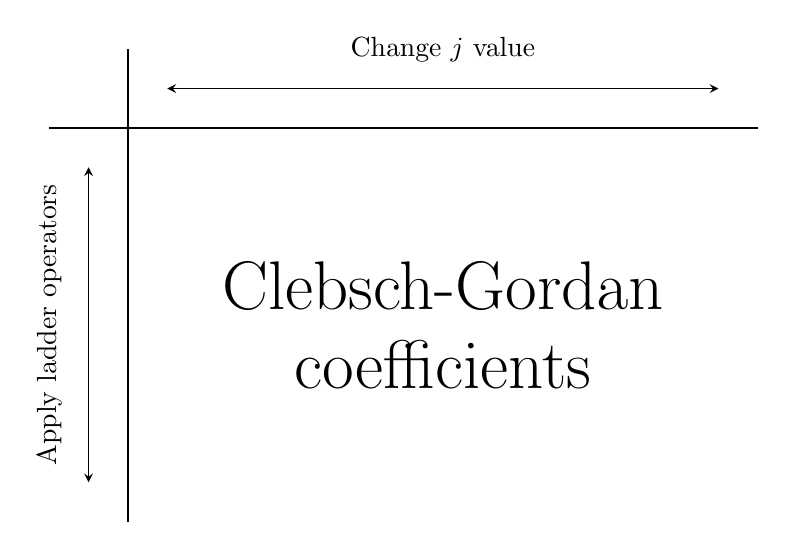
\begin{tikzpicture}
\draw[thick] (-1,0) -- (8,0);
\draw[thick] (0,1) -- (0,-5);
\draw[<->] (0.5,0.5) -- (7.5,0.5);
\node at (4,1) {Change $j$ value};
\draw[<->] (-0.5,-0.5) -- (-0.5,-4.5);
\node[rotate=90] at (-1,-2.5) {Apply ladder operators};
\node at (4,-2) {\Huge{Clebsch-Gordan}};
\node at (4,-3) {\Huge{coefficients}};
\end{tikzpicture}
\end{center}

\subsection{Value of $m$}

Consider the action of $J_3$ on both bases, 
\bi{rCl}
J_3\xi_{j,j_A,j_B}^m & = & m\xi_{j,j_A,j_B} \\
J_3 (\alpha_{j_A}^{m_a} \otimes \beta_{j_B}^{m_B}) & = & (m_A+m_B)(\alpha_{j_A}^{m_a} \otimes \beta_{j_B}^{m_B}).
\ei 
Then, from the fact that the CGcs are simply complex numbers and the fact that $J_3$ is linear, it follows from the expansion equation that we require 
\bse 
m = m_A + m_B.
\ese 
In other words, whenever $m\neq m_A+m+B$, we require that the CGc vanishes. We can, therefore, place this as a constraint on our summands giving us 
\bse 
\xi_{j,j_A,j_B}^m = \sum_{\substack{m_A,m_B \\ m_A+m_B=m}} C_{j,j_A,j_B}^{m,m_A,m_B} (\alpha_{j_A}^{m_a} \otimes \beta_{j_B}^{m_B}),
\ese 
where we have left the ranges of $m_A/m_B$ out, but they are of course just $-j_A,...,j_A$ and $-j_B,...,j_B$.

\subsection{Clebsch-Gordan Coefficients for Maximal $j$}

We are now in a position to choose our convenient initial eigenvector. It follows from the ranges of $m_A$ and $m_B$ along with the condition $m=m_A+m_B$ and $m=-j,...,j$ that the maximum value $j$ can take is $j_A+j_B$. It follows then that 
\bse 
\xi_{j_A+j_B,j_A,j_B}^{j_A+j_B} = C_{j_A+j_B,j_A,j_B}^{j_A+j_B,j_A,j_B} (\alpha_{j_A}^{j_A}\otimes\beta_{j_B}^{j_B}),
\ese 
and all other CGcs at the level $C_{j_A+j_B,j_A,j_B}^{j_A+j_B, -, -}$ vanish. Then from the fact that both eigenbases are normalised we know that 
\bse 
\big|C_{j_A+j_B,j_A,j_B}^{j_A+j_B,j_A,j_B}\big|^2 = 1,
\ese 
and so the two eigenvectors vary only by a complex phase. However, seeing as we are only interested in eigenvalues here, and an \emph{overall} phase plays no effect on the eigenvalue, we are free to set this phase however we like. We choose it such that 
\bse 
C_{j_A+j_B,j_A,j_B}^{j_A+j_B,j_A,j_B} = 1.
\ese 

We can now start applying the ladder operators to lower the value of $m=j_A+j_B$. Using \Cref{prp:LadderCoefficients} we have 
\bi{rCl}
J_- \xi_{j_A+j_B,j_A,j_B}^{j_A+j_B} & = & \sqrt{(j_A+j_B)(j_A+j_B+1)-(j_A+j_B)(j_A+j_B-1)}\xi_{j_A+j_B,j_A,j_B}^{j_A+j_B-1} \\
& = & \sqrt{2(j_A+j_B)}\xi_{j_A+j_B,j_A,j_B}^{j_A+j_B-1}
\ei 
However we equally have 
\bi{rCl}
J_-(\alpha_{j_A}^{j_A}\otimes\beta_{j_B}^{j_B}) & = & (A_-\otimes\b1 +\b1\otimes B_-) (\alpha_{j_A}^{j_A}\otimes\beta_{j_B}^{j_B}) \\
& = & \sqrt{2j_A}(\alpha_{j_A}^{j_A-1}\otimes\beta_{j_B}^{j_B}) + \sqrt{2j_B}(\alpha_{j_A}^{j_A}\otimes\beta_{j_B}^{j_B-1}).
\ei
Then, equating these two, we obtain 
\bi{rCl}
C_{j_A+j_B,j_A,j_B}^{j_A+j_B-1,j_A-1,j_B} & = & \sqrt{\frac{j_A}{j_A+j_B}} \\
C_{j_A+j_B,j_A,j_B}^{j_A+j_B-1,j_A,j_B-1} & = & \sqrt{\frac{j_B}{j_A+j_B}},
\ei 
with all other CGcs at this level vanishing. 

We can repeat this process to obtain the CGcs at the level $C_{j_A+j_B,j_A,j_B}^{j_A+j_B-2,-,-}$, and iterate until we reach $m=-(j_A+j_B)$, which is where it must terminate. 

\subsection{Clebsch-Gordan Coefficients For Lower Than Max $j$}

We now wish to reduce $j$ itself to produce the second column of our table. We first need to ask what the next highest allowed $j$ value is. Recalling that $j\in\N_0/2$ we might try $j_A+j_B-1/2$, however this is not allowed. The answer to why follows simply from the fact that $j_A$ and $j_B$ themselves are fixed, so all we can change is $m_A$ and $m_B$, which must change in integer steps. Combining this with the $m=m_A+m_B$, which holds generally, we would not be able to get $m=-j,...,j$. That is, the next CGcs are of level $C_{j_A+j_B-1,j_A,j_B}^{j_A+j_B-1,-,-}$. Then using the fact that there are only two ways to obtain this (either $m_A\to m_A-1$ or $m_B\to m_B-1$) we have 
\bse 
\xi_{j_A+j_B-1,j_A,j_B}^{j_A+j_B-1} = C_{j_A+j_B-1,j_A,j_B}^{j_A+j_B-1,j_A-1,j_B}(\alpha_{j_A}^{j_A-1}\otimes\beta_{j_B}^{j_B}) + C_{j_A+j_B-1,j_A,j_B}^{j_A+j_B-1,j_A,j_B-1}(\alpha_{j_A}^{j_A}\otimes\beta_{j_B}^{j_B-1}).
\ese 

We then use the fact that the eigenvectors in this equation are all orthonormal to obtain 
\bse 
1 = \big|C_{j_A+j_B-1,j_A,j_B}^{j_A+j_B-1,j_A-1,j_B}\big|^2 + \big|C_{j_A+j_B-1,j_A,j_B}^{j_A+j_B-1,j_A,j_B-1}\big|^2,
\ese 
and we also use the fact that the RHS eigenvectors are the same here as with the $J_-$ case above however the LHS eigenvectors are necessarily orthogonal to give 
\bi{rCl} 
\overline{C_{j_A+j_B,j_A,j_B}^{j_A+j_B-1,j_A-1,j_B}}\cdot C_{j_A+j_B-1,j_A,j_B}^{j_A+j_B-1,j_A-1,j_B} & = & - \overline{C_{j_A+j_B,j_A,j_B}^{j_A+j_B-1,j_A,j_B-1}}\cdot C_{j_A+j_B-1,j_A,j_B}^{j_A+j_B-1,j_A,j_B-1} \\
\sqrt{\frac{j_A}{j_A+j_B}}\cdot C_{j_A+j_B-1,j_A,j_B}^{j_A+j_B-1,j_A-1,j_B} & = & -\sqrt{\frac{j_B}{j_A+j_B}}\cdot C_{j_A+j_B-1,j_A,j_B}^{j_A+j_B-1,j_A,j_B-1} \\
C_{j_A+j_B-1,j_A,j_B}^{j_A+j_B-1,j_A-1,j_B} & = & -\sqrt{\frac{j_B}{j_A}}\cdot  C_{j_A+j_B-1,j_A,j_B}^{j_A+j_B-1,j_A,j_B-1}.
\ei 

Solving simultaneously, 
\bi{rCl}
\bigg(\frac{j_B}{j_A} +1\bigg)\big|C_{j_A+j_B-1,j_A,j_B}^{j_A+j_B-1,j_A,j_B-1}\big|^2 & = & 1 \\
\big|C_{j_A+j_B-1,j_A,j_B}^{j_A+j_B-1,j_A,j_B-1}\big| & = & \sqrt{\frac{j_A}{j_A+j_B}} \\
\implies \big|C_{j_A+j_B-1,j_A,j_B}^{j_A+j_B-1,j_A-1,j_B}\big| & = & -\sqrt{\frac{j_B}{j_A+j_B}}
\ei 
Finally we just fix the phases as we want to give 
\bse
C_{j_A+j_B-1,j_A,j_B}^{j_A+j_B-1,j_A,j_B-1} = \sqrt{\frac{j_A}{j_A+j_B}}, \qquad \qquad  C_{j_A+j_B-1,j_A,j_B}^{j_A+j_B-1,j_A-1,j_B} = -\sqrt{\frac{j_B}{j_A+j_B}}.
\ese

We can then apply the $J_-$ operator as before to move down this column. We can repeat this process of lowering $j$ again to obtain the third column, and iterate until we reach $j=|j_A-j_B|$, where it must terminate. We see that this is the termination point quickly from $m=-j,...,j$ along with $m=m_A+m_B$. On the next page I have included a table (from David J. Griffiths' QM book) for some calculated CGcs. As we can see... they're not pretty things.

\subsection{Total Spin of Composite System}

We conclude, then, that in quantum mechanics when we want to compose a spin-$j_A$ system with a spin-$j_B$ system we do \emph{not} just get a spin-$j_A+j_B$ system, but instead we get the direct sum 
\bse
(\text{spin-}_{j_A+j_B}) \oplus (\text{spin-}_{j_A+j_B-1}) \oplus ... \oplus (\text{spin-}_{|j_A-j_B|}).
\ese 

\begin{center}
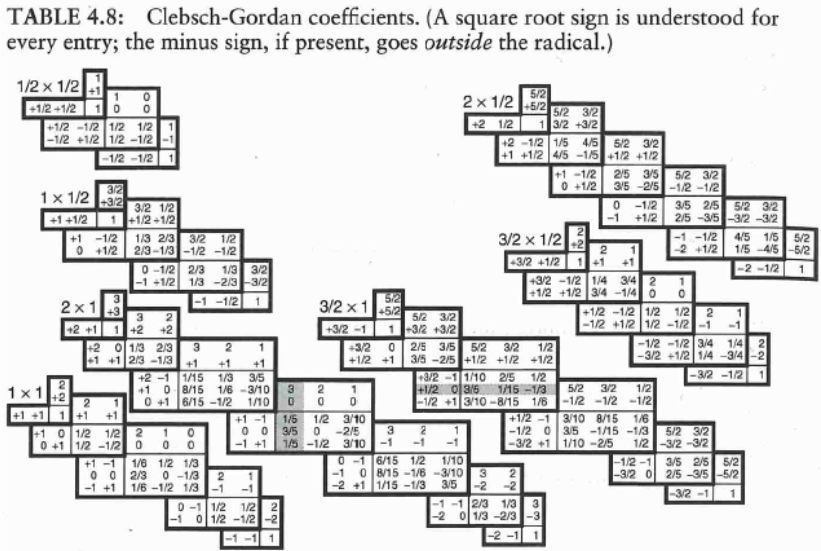
\includegraphics[scale=0.7,angle=90, origin=c]{graphics/ClebschGordan.png}
\end{center}
\newpage

\section{Quantum Harmonic Oscillator}
As has been remarked, the world and everything in it are quantum by nature. There is no `classical' ball which we make quantum, there is a quantum ball that we approximate classically. Equally there isn't a `classical' harmonic oscillator which we use to construct the quantum one. We will thus \emph{not} entertain any type of so called `\emph{quantisation}' idea --- that of starting from the classical system and somehow transforming it into the quantum counter part. We shall demonstrate explicitly in the first section why this is not a good idea, but a quick argument explains it.

Imagine you have some general theory. Of course you can obtain any special theory related to it by taking approximations/constraints, however you have no real hope of doing the opposite --- you should not expect to be able to obtain the general theory by `unapproximating' the special one. Quantum mechanics is the general theory, with classical mechanics is the special one. It is therefore a ridiculous idea to try and obtain quantum theory this way.

\subsection{What People Say}

Despite the clear message above, people still choose to do such a thing; they take the equations governing a system classically and `replace them' with the quantum versions. To be fair, it is not that the physics community are unaware of the above fact, it is simply that they argue `we only do it in special cases where we know no problems arise.' 

However, even in said special circumstances, we argue, it is still a terribly misleading and potentially devastating (theoretically speaking!) idea. We shall quickly highlight why this is. 

The procedure is as follows. Take the function representing your classical observable $f(p,q)$, where $p$ is the position and $q$ the momentum, and simply rewrite the function but replacing $p$ with the quantum mechanical operator $P$ and $q$ with $Q$.
\bse 
f(p,q) \squiggle f(P,Q)
\ese 

For example the energy observable for the harmonic oscillator 
\bse 
h(p,q) = \frac{1}{2m}p^2+\frac{m\omega^2}{2}q^2 \squiggle H := h(P,Q) = \frac{1}{2m}P\circ P + \frac{m\omega^2}{2}Q\circ Q 
\ese 
It follows from 
\bse
P,Q : S(\R) \to S(\R),
\ese  
with 
\bse 
(P\psi)(x) := -i\hbar \psi'(x), \qquad  (Q\psi)(x) := x\psi(x),
\ese 
that 
\bse
H : S(\R) \to S(\R),
\ese  
with 
\bse 
(H\psi)(x) := -\frac{\hbar^2}{2m}\psi''(x) +\frac{m\omega^2}{2}x^2\psi(x).
\ese 
This often appears as 
\bse 
H := -\frac{\hbar^2}{2m}\frac{d^2}{dx^2} +\frac{m\omega^2}{2}x^2,
\ese 
or for a more general case (i.e. not a harmonic oscillator) as 
\bse 
H := -\frac{\hbar^2}{2m}\frac{d^2}{dx^2} + V(x),
\ese 
where $V(x)$ is the potential associated to the system.

This all looks very nice, and indeed it is correct, however there is a serious problem here. Classically we could add 
\bse 
(pq-qp)g(p,q),
\ese 
for some other observable of the system $g(p,q)$ without changing anything, as the bracket vanishes. That is 
\bse 
f(p,q) = f(p,q) + (pq-qp)g(p,q).
\ese 
However if we then applied the `$\squiggle$' approach to this we would get 
\bse 
f(P,Q) = f(P,Q) + [P,Q]g(P,Q) = f(P,Q) + i\hbar g(P,Q),
\ese 
which is obviously not true for general $g(P,Q)$. So it appears that even in these simple cases where `there is no danger', there is a serious theoretical problem. For this reason we shall just not do this at all, and instead simply define what we mean by the energy observable (or \emph{Hamiltonian}) of our system and proceed from there. 

\subsection{The Quantum Harmonic Oscillator}
In keeping with Axiom 1, we need an underlying Hilbert space; we use $\cH=L^2(\R)$. We also have (in agreement with Axiom 4) an energy observable, known as the Hamiltonian of the system,
\bse 
H := \frac{1}{2m}P\circ P + \frac{1}{2}m\omega^2 Q\circ Q.
\ese 

However, a note must be made. If $H$ is to be an observable, it must be self adjoint. But in the above expression we have used the essentially self adjoint $Q,P:S(\R)\to S(\R)$. This is not a large worry as we can simply take their unique self adjoint extensions. We still have a problem though. Although $P\circ P$ and $Q\circ Q$ (as the self adjoint extensions) will be self adjoint, their \emph{sum} need not be, as the adjoint does not necessarily distribute across the addition. 

What we shall do is consider the essentially self adjoint operators throughout, and then at the end we shall present Theorem that allows us to conclude that $H$ (constructed from the essentially self adjoint operators) is essentially self adjoint, and so a unique self adjoint extension exists. 

As above, we shall not employ a different notation for the self adjoint and essentially self adjoint operators, but instead infer which we are dealing with by considering the domains. 

\subsection{The Energy Spectrum}

Recall that the spectrum of an operator is given by
\bse 
\sigma(H) = \sigma_p(H) \cup \sigma_c(H).
\ese 
The aim of this lecture is to calculate $\sigma_p(H)$ and show that $\sigma_c(H)=\varnothing$. 

\bd 
Consider the operators $Q,P:S(\R)\to S(\R)$. Then define $a_{\pm} : S(\R) \to S(\R)$ via
\bse 
a_{\pm} := \sqrt{\frac{m\omega}{2\hbar}} Q \mp \frac{i}{\sqrt{2\hbar m \omega}} P.
\ese 
\ed 

\bc 
We can re-express the Hamiltonian as 
\bse 
H = \hbar \omega \bigg( a_+a_- + \frac{1}{2}\id_{S(\R)}\bigg).
\ese 
\ec 

\bq 
The proof follows from direct substitution. Let 
\bse 
\alpha := \sqrt{\frac{m\omega}{2\hbar}}, \qquad \beta := \frac{1}{\sqrt{2\hbar m \omega}}
\ese 
\bi{rCl}
H & = & \hbar\omega \bigg((\alpha Q - i\beta P)(\alpha Q + i\beta P) +\frac{1}{2}\id_{S(\R)}\bigg) \\
& = & \hbar\omega \bigg( \alpha^2Q\circ Q + \beta^2P\circ P + i\alpha\beta (QP-PQ) + \frac{1}{2}\id_{S(\R)}\bigg) \\
& = & \hbar\omega \bigg( \alpha^2 Q\circ Q + \beta^2 P\circ P + i\alpha\beta [Q,P] + \frac{1}{2}\id_{S(\R)}\bigg) \\
& = &  \hbar\omega\bigg( \frac{m\omega}{2\hbar}Q\circ Q + \frac{1}{2\hbar m\omega} P \circ P + i \frac{1}{2\hbar} (i\hbar)\id_{S(\R)} + \frac{1}{2}\id_{S(\R)}\bigg) \\
& = & \frac{1}{2m}P\circ P + \frac{m\omega^2}{2}Q \circ Q,
\ei 
where we have used $[Q,P]=i\hbar\id_{S(\R)}$.
\eq 

\bp 
The following commutation relations hold:
\ben[label=(\roman*)]
\item $[a_-,a_+]=\id_{S(\R)}$,
\item $[H,a_+]=\hbar\omega a_+$,
\item $[H,a_-]=-\hbar\omega a_-$.
\een 
\ep 

\bq 
They all follow from direct substitution, using $H$ as written in the previous Corollary. 
\ben[label=(\roman*)]
\item \bi{rCl}
[a_-,a_+] & = & [\alpha Q+i\beta P, \alpha Q -i\beta P] \\
& = & \alpha^2[Q,Q] -i\alpha\beta [Q,P] + i\beta\alpha[P,Q] +\beta^2[P,P] \\
& = & -i2\alpha\beta [Q,P] \\
& = & -i2\alpha\beta (i\hbar)\id_{S(\R)} \\
& = & \frac{2\hbar}{2\hbar} \id_{S(\R)} \\
& = & \id_{S(\R)},
\ei 
where we have made use of the linearity of the commutator bracket. 
\item \bi{rCl}
[H,a_+] & = & \bigg[\hbar\omega a_+a_- +\frac{1}{2}\id_{S(\R)}, a_+\bigg] \\
& = & \hbar\omega [a_+a_-,a_+] + \frac{1}{2}[\id_{S(\R)},a_+] \\
& = & \hbar\omega \big( a_+[a_-,a_+] + [a_+,a_+]a_-\big) \\
& = & \hbar\omega a_+\id_{S(\R)} \\
& = & \hbar\omega a_+
\ei 
\item This follows exactly analogously to (ii).
\een 
\eq 

\br 
Strictly speaking in the previous proof we should have considered the action of the commutator on an element of $S(\R)$ and showed that the expressions hold for an arbitrary element. Doing it this way will return the same results, however this will not always be true, and so care must be taken in future.
\er 

There are four more basic facts that allow us to obtain the spectrum in its entirety. We claim that, for the $H$-eigenvalue $\psi$, the following hold:
\ben[label=(\roman*)]
\item $H(a_+\psi) = (E+\hbar\omega)(a_+\psi)$, 
\item $\|a_+\psi\| \geq \|\psi\| > 0$,
\item $H(a_-\psi) = (E-\hbar\omega)(a_-\psi)$,
\item $E\geq \frac{1}{2}\hbar\omega$.
\een 

\bq 
\ben[label=(\roman*)]
\item From the previous result we have
\bi{rCl}
H(a_+\psi) & = & a_+(H\psi) + [H,a_+]\psi \\
& = & Ea_+\psi + \hbar\omega a_+\psi \\
& = & (E+\hbar\omega)(a_+\psi)
\ei 
\item Given that $(a_+)^* = a_-$ and vice versa,\footnote{To show this you need to consider the definition of the adjoint and work from there, as you don't know that it will distribute across the addition in the definitions.}
\bi{rCl}
\|a_+\psi\|^2 & = & \braket{a_+\psi}{a_+\psi} \\
& = & \braket{\psi}{(a_+)^*a_+\psi} \\
& = & \braket{\psi}{a_-a_+\psi} \\
& = & \braket{\psi}{a_+a_-\psi} + \braket{\psi}{[a_-,a_+]\psi} \\
& = & \braket{a_-\psi}{a_-\psi} + \braket{\psi}{\id_{S(\R)}\psi} \\
& \geq & \braket{\psi}{\psi} \\
& = & \|\psi\|^2,
\ei 
where we used the fact that the inner product is non-negative definite in the second to last last step (i.e. the first term is non-negative). The result follows from taking the square root and imposing the condition that the norm is non-negative definite.
\item This is done exactly analogously to (i). 
\item Consider 
\bi{rCl}
E\braket{\psi}{\psi} & = & \braket{\psi}{E\psi} \\
& = & \braket{\psi}{H\psi} \\
& = & \hbar\omega \bigg(\braket{\psi}{a_+a_-\psi} + \frac{1}{2}\braket{\psi}{\id_{S(\R)}\psi} \bigg) \\
& = & \hbar\omega\bigg( \braket{a_-\psi}{a_-\psi} + \frac{1}{2}\braket{\psi}{\id_{S(\R)}\psi} \bigg) \\ 
& \geq & \frac{\hbar\omega}{2}\braket{\psi}{\psi}. 
\ei 
Then from the fact that $\psi$ is an eigenvector (and so cannot be the zero vector), the inner product is non-vanishing and we can divide through by it, giving the result.
\een 
\eq 

We can, thus, draw some conclusions. For any $H$-eigenvector, $\psi$, with eigenvalue $E$ we have:
\ben 
\item From (i) and (ii) it follows that $a_+\psi$ is a eigenvector, as (i) tells us it obeys the eigenvalue equation and (ii) tells us its not the zero vector. Thus we know that the sequence 
\bse 
\{(a_+)^n\psi\}_{n\in\N_0}
\ese 
where the power indicates $n$-th order composition of operators, is a sequence of eigenvectors with correspoding eigenvalues 
\bse 
\{E + n\hbar\omega\}_{n\in\N_0}.
\ese 
\item (iii) and (iv) tell us that the sequence of eigenvectors
\bse 
\{(a_-)^n\psi\}_{n\in\N_0}
\ese 
\emph{must} terminate for some $n=N\in\N$. That is, we can not continue to keep lowering the eigenvalue $E$ forever, as (iv) says it bounded from below. Note this tells us that $a_-\psi$ is \emph{not} strictly a $H$-eigenvalue (just as $J_{\pm}$ weren't for $\Omega$ and $J_3$).

In other words there is a non-vanishing $\psi_0\in S(\R)$ defined as 
\bse 
\psi_0 := (a_-)^N\psi
\ese 
such that $a_-\psi = 0_{S(\R)}$. It follows, then, from the definition of the Hamiltonian that 
\bi{rCl}
H\psi_0 & = & \hbar\omega a_+a_-\psi_0 + \frac{\hbar\omega}{2}\psi_0 \\
& = & \frac{\hbar\omega}{2}\psi_0,
\ei 
and so it has the lowest possible eigenvalue, by (iv). 
\item The entire sequence (as defined above) of eigenvalues is 
\bse 
\bigg\{ \hbar\omega \bigg(n+\frac{1}{2}\bigg)\bigg\}_{n\in\N_0}.
\ese 
Equivalently, we say the $n$-th eigenvector 
\bse 
\psi_n := (a_+)^n\psi 
\ese 
has the corresponding eigenvalue
\bse 
E_n := \hbar\omega \bigg(n+\frac{1}{2}\bigg)
\ese 
\item Considering again $a_-\psi_0=0_{S(\R)}$ along with the definition of $a_-$ we have 
\bse 
\bigg( \sqrt{\frac{m\omega}{2\hbar}}x + i \frac{1}{\sqrt{2\hbar m\omega}} (-i\hbar)\frac{d}{dx}\bigg)\psi_0(x) = 0,
\ese 
which is just a ODE. We can solve this using separation of variables; rearranging, we have
\bse
\psi_0'(x) = -\frac{m\omega}{\hbar} x\psi_0(x), 
\ese 
which using standard separation of variables technique gives 
\bi{rCl}
\ln|\psi_0(x)| & = & -\frac{m\omega}{2\hbar}x^2 + C \\
\psi_0(x) & = & \pm e^C e^{-\frac{m\omega}{2\hbar}x^2} \\
\psi_0(x) & = & A e^{-\frac{m\omega}{2\hbar}x^2},
\ei 
for complex constants $C$ and $A:=\pm e^C$. 

Imposing a normalisation condition, we can then write the $n$-th eigenvector in terms of the $n$-th \emph{Hermit polynomial}, $H_n$, as 
\bse 
\psi_n \propto H_n\bigg(\sqrt{\frac{m\omega}{\hbar}}x\bigg) e^{-\frac{m\omega}{2\hbar}x^2}.
\ese 
\een

\bc 
From 4. we note that (up to the usual ambiguity of a complex multiple) there is only one eigenvector to each eigenvalue. That is we have the 1-dimensional eigenspace
\bse 
\text{Eig}_{H}(E_n) = \text{span}_{\C}(\psi_n),
\ese 
which tells us not only that $\psi_0$ exists in the first place, but that it is unique. 
\ec 

\br
At the end of the last corollary we said that we confirmed the existence of $\psi_0$ in the first place. This might seem like a strange comment given the whole calculation, however it is actually rather important. To illustrate why Dr. Schuller mentions a doctoral proposal he once saw in which the student had derived some truly impressive formulae, only to have someone point out that towards the start of his calculation he had 0, and so everything that followed could have just been a repercussion of that (i.e. $0\cdot n = 0$ for any $n$ in your space). It is therefore to check that the things you are using actually exist, in this case $\psi_0$ doesn't vanish and so is an eigenvector. 
\er 

The Hermit polynomial expression is equally an important result as it tells us that $\psi_n\in S(\R)$ (as all polynomials are in $S(\R)$), which it needs to be if we are to act on it with our operators. Moreover, one can show that the set 
\bse 
\{\psi_n \, | \, n\in\N_0\}
\ese 
is an ON-eigenbasis for $L^2(\R)$, which leads us to the theorem promised at the start of the lecture.

\bt 
If a symmetric operator has as its eigenvectors an ON-basis, the operator is guaranteed to be essentially self adjoint. 
\et 

This theorem tells us that $H$ is essentially self adjoint, and the fact that we have an ON-eigenbasis for $L^2(\R)$ tells us that the continuous spectrum is empty. 
\newpage

\section{Measurements of Observables}
So far we have discussed the spectrum of an observable, which tells us all the \emph{possible} measurement outcomes, but tells us nothing about the actual act of taking a measurement itself. This comes through axioms 3 and 5. In order to illustrate these two axioms we will repeatedly use the quantum harmonic oscillator as an example, but it is important to note the methods are not specific to this case. Any restrictions required for the methods to hold will be clearly stated. 

This lecture can be read in two ways. One could read sections 4 and 5 first (on how you prepare a given state) and then return to read sections 1-3 (on how you take measurements of this state); or one could simply read it as presented (i.e. 1-5). Both reading orders have their advantages, but we present it here in the order taught by Dr. Schuller. Also in correspondence with the lecture given, we shall also translate some of the notation into the commonly used bra-ket notation (see lecture 4), even though we do not use it in this course. All these expressions shall appear in blue. 

\subsection{Spectral Decomposition of $H$ For The Quantum Harmonic Oscillator}

Recall: We found an ON-basis of $H$-eigenvalues which we labelled $\psi_n$ obeying 
\bse 
H\psi_n = E_n\psi_n,
\ese 
with 
\bse 
E_n = \hbar\omega \bigg(n+\frac{1}{2}\bigg).
\ese 
More precisely we derived 
\bse 
\psi_0(x) = \sqrt{\frac{m\omega}{2\hbar}}\exp\bigg(-\frac{m\omega}{2\hbar}x^2\bigg),
\ese 
and 
\bse 
\psi_n(x) := A_n (a_+)^n\psi_0(x) \propto H_n\bigg(\sqrt{\frac{m\omega}{\hbar}}x\bigg)\exp\bigg(-\frac{m\omega}{2\hbar}x^2\bigg).
\ese 

The only thing we will actually use in this lecture is the fact that the $\{\psi_n\}$ is an ON-basis,
\bse 
\braket{\psi_n}{\psi_m} = \delta_{nm},
\ese 
and the fact that the spectrum is given by 
\bse 
\sigma(H) = \bigg\{ \hbar\omega\bigg(n+\frac{1}{2}\bigg)\, \Big| \, n\in\N_0\bigg\}.
\ese 

The key to understanding measurement theory in quantum mechanics is that you know the spectral decomposition of the observable(s) you want to measure. In order to obtain the spectral decomposition of $H$ we consider the projectors 
\bse 
P_n(\cdot) := \braket{\psi_n}{\cdot} \psi_n \textcolor{blue}{= \ket{\psi_n}\bra{\psi_n}.}
\ese 
Note that this operator is bounded as 
\bse 
\sup_{\varphi\in\cH}\frac{\|P_n(\varphi)\|_{\cH}}{\|\varphi\|^2_{\cH}} = \sup_{\varphi\in\cH}\frac{|\braket{\psi_n}{\varphi}|^2\|\psi_n\|^2}{\|\varphi\|^2} = \sup_{\varphi\in\cH}\frac{|\braket{\psi_n}{\varphi}|^2}{\|\varphi\|^2} < \infty.
\ese 
We can, therefore, employ the operator norm on $\cL(\cH)$ to decide convergence of the following sum with the result
\bse 
\sum_{n=0}^{\infty} P_n = \id_{\cH}.
\ese 

\bd 
For every Borel set $\Omega\in\R$, define 
\bse 
P_H(\Omega) := \sum_{\substack{n \\ E_n\in\Omega}} P_n,
\ese 
i.e. the sum over the projectors such that the energy eigenvalue corresponding to the state\footnote{Again recall $\psi_n$ are not the states themselves, $\rho_{\psi_n}$ are} corresponding to $\psi_n$ is within your Borel set. 
\ed 

\br 
From now on we shall drop the $E_n\in\Omega$ on the sum, to lighten the notation, but it is important to remember that it belongs there whenever we use $P_H$. It will prove highly instrumental to the results that follow. 
\er 

\be 
Let $\Omega=\{E_m\}$, i.e. just the set containing the single eigenvalue $E_m$. Clearly then 
\bse 
P_H(\Omega) = P_m.
\ese 
\ee 

\be 
Let $\Omega=\{E_m,E_k\}$. Then we have 
\bse 
P_H(\Omega) = P_m + P_k.
\ese 
\ee 

\bp 
The map $P_H:\sigma(\R)\to\cL(\cH)$ is a projection valued measure, and in fact corresponds to \emph{the} projection valued measure that appears in the spectral theorem for $H$. That is 
\bi{rCl}
H & = & \int_{\R}\lambda P_H(d\lambda) \\
& = & \sum_{n=0}^{\infty} E_n \cdot P_n \\
& \textcolor{blue}{=} & \textcolor{blue}{\sum_{n=0}^{\infty}\hbar\omega\bigg(n+\frac{1}{2}\bigg)\ket{\psi_n}\bra{\psi_n}}.
\ei 
\ep 

\br 
The above proposition makes sense. The Hamiltonian (the energy operator) is given by the energy eigenvalues multiplied by a projector that projects the state into a state whose energy eigenvalue was the prefactor. This is clearly just the eigenvector equation.
\er 

\br 
Note there was nothing specifically special about the fact that we were considering the Hamiltonian above. Indeed the same method holds for \emph{any} observable you wish to measure. First find an ON-basis of eigenvectors for your operator, $A$ say, and then define the PVM associated to the observable
\bse 
P_A:\sigma(\R) \to \cL(\cH)
\ese 
in the same way and then plug it into the spectral theorem. 
\er 

\subsection{Probability to Measure a Certain Value}

As stated in the opening of this lecture, the method is the same for all observables and their measurements, but we shall use the energy of the quantum harmonic oscillator as our working example. 

Recall, the spectrum of $H$ is the set of principally possible measurement outcome results. We want to show this pictorially, as it will help with understanding what's to follow. 

As we measuring anything in the real world, we need some kind of measuring device. You feed in the thing you want to take a measurement of and the meter on the device tells you the measurement value. The one slightly different, but highly important, difference to note with quantum mechanics is that the device potentially alters the thing you were measuring. We shall draw this as follows. 

\begin{center}
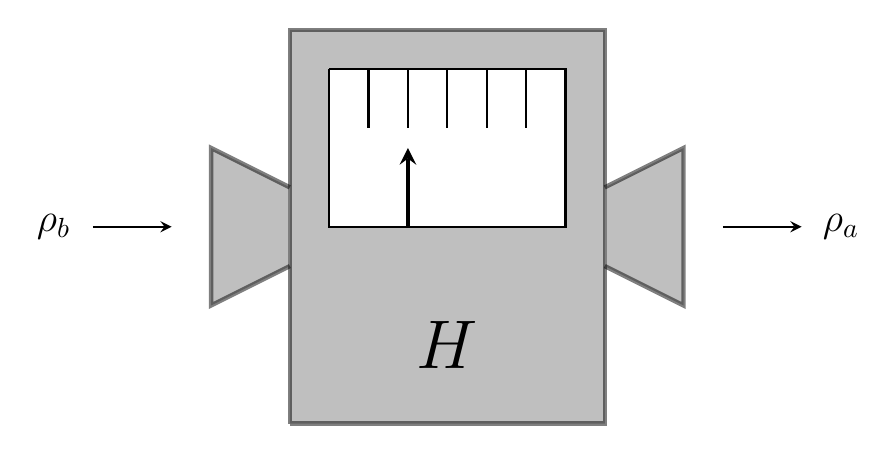
\begin{tikzpicture}
\draw[ultra thick,  fill=gray, opacity=0.5] (0,0) -- (4,0) -- (4,5) -- (0,5) -- (0,0);
\draw[ultra thick,  fill=gray, opacity=0.5] (0,2) -- (-1,1.5) -- (-1,3.5) -- (0,3);
\draw[ultra thick,  fill=gray, opacity=0.5] (4,2) -- (5,1.5) -- (5,3.5) -- (4,3);
\draw[thick, fill=white] (0.5,4.5) -- (3.5,4.5) -- (3.5,2.5) -- (0.5,2.5) -- (0.5,4.5);
\draw[thick] (1,4.5) -- (1,3.75);
\draw[thick] (1.5,4.5) -- (1.5,3.75);
\draw[thick] (2,4.5) -- (2,3.75);
\draw[thick] (2.5,4.5) -- (2.5,3.75);
\draw[thick] (3,4.5) -- (3,3.75);
\draw[ultra thick,->] (1.5,2.5) -- (1.5,3.5);
%%%%
\node at (2,1) {\Huge{$H$}};
\draw[thick, ->] (-2.5,2.5) -- (-1.5,2.5);
\draw[thick, ->] (5.5,2.5) -- (6.5,2.5);
\node at (-3,2.5) {\Large{$\rho_b$}};
\node at (7,2.5) {\Large{$\rho_a$}};
\end{tikzpicture}
\end{center}

The $H$ tells us that it is the device associated to the observable $H$, the scale markings tell us the spectrum\footnote{Here we are considering the spectrum of the harmonic oscillator, and so the notches are evenly spaced. Clearly this will not always be true. In general we have notches of varying separation as well as `blocks' for the continuous parts of the spectrum.}, the arrow tells us the \emph{actual} measurement made, $\rho_b$ is the state before the measurement and $\rho_a$ is the state after the measurement. 

\br 
Note that the pointer here will not move continuously between the notches; it moves between the values by jumping between them. In other words, it can no point at in between two notches, as this would not be part of the spectrum. 
\er 

Recall: a \emph{state} of a quantum system is a self adjoint operator that is:
\ben[label=(\roman*)]
\item Trace-class: $\Tr(\rho)=\sum_{e_n}\braket{e_n}{\rho(e_n)} <\infty$, where $\{e_n\}$ is \emph{any} ON-basis. 
\item Unit trace: $\Tr(\rho)=1$. 
\item Positive: $\forall\varphi\in\cH, \, \braket{\varphi}{\rho(\varphi)}\geq 0$.\footnote{Note that this should really be called `non-negative', however this is just how it is named.}
\een 

Also recall: Axiom 3 assorts that the probability to obtain a measurement outcome (a `pointer position') within a Borel set $\Omega$ when measuring an observable $H$ on a system in state $\rho$ is given by
\bse 
\Tr\big(P_H(\Omega)\circ \rho\big),
\ese 
where $P_H$ is the unique PVM from the spectral decomposition of $H$. In terms of our picture it asks the question `What is the probability that the pointer points within the range $\Omega$ on the scale?'
\begin{center}
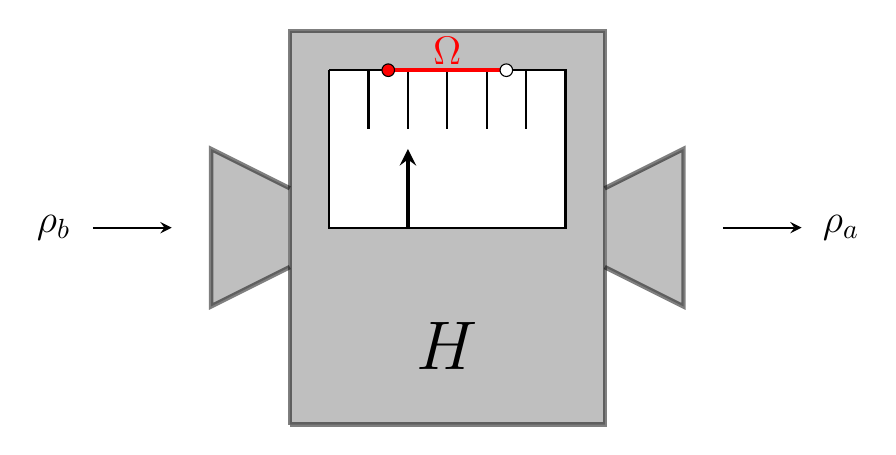
\begin{tikzpicture}
\draw[ultra thick,  fill=gray, opacity=0.5] (0,0) -- (4,0) -- (4,5) -- (0,5) -- (0,0);
\draw[ultra thick,  fill=gray, opacity=0.5] (0,2) -- (-1,1.5) -- (-1,3.5) -- (0,3);
\draw[ultra thick,  fill=gray, opacity=0.5] (4,2) -- (5,1.5) -- (5,3.5) -- (4,3);
\draw[thick, fill=white] (0.5,4.5) -- (3.5,4.5) -- (3.5,2.5) -- (0.5,2.5) -- (0.5,4.5);
\draw[thick] (1,4.5) -- (1,3.75);
\draw[thick] (1.5,4.5) -- (1.5,3.75);
\draw[thick] (2,4.5) -- (2,3.75);
\draw[thick] (2.5,4.5) -- (2.5,3.75);
\draw[thick] (3,4.5) -- (3,3.75);
\draw[ultra thick,->] (1.5,2.5) -- (1.5,3.5);
%%%%
\node at (2,1) {\Huge{$H$}};
\draw[thick, ->] (-2.5,2.5) -- (-1.5,2.5);
\draw[thick, ->] (5.5,2.5) -- (6.5,2.5);
\node at (-3,2.5) {\Large{$\rho_b$}};
\node at (7,2.5) {\Large{$\rho_a$}};
%%%%
\draw[ultra thick, red] (1.25,4.5) -- (2.75,4.5);
\draw[fill=red] (1.25,4.5) circle [radius=0.08];
\draw[fill=white] (2.75,4.5) circle [radius=0.08];
\node at (2,4.75) {\textcolor{red}{\Large{$\Omega$}}};
\end{tikzpicture}
\end{center}

\br 
We wish to emphasise this point again here. The spectrum of an observable only tells you the \emph{possible} measurements and the results of last lecture give you information on the \emph{probability} of each possible measurement. This is where the probabilistic nature enters into quantum mechanics. When a measurement is made, the result is concrete. You get exactly that result. This in tern effects the state of your system, giving a (potentially) new state. This is where the indeterminate nature of quantum mechanics enters. 

That is, prior to the measurement you can only say with what probability you get one of the possible final states, but once the measurement is made, it is exactly that one, and which final state you get depends on which measurement result you get. This is the \emph{quantum} behaviour of the system. 

As we shall see in section 5 there is another form of probability concerned with quantum mechanics, but this probability does not stem from the quantum nature of the system itself. It stems from the `ignorance' of the experimenter/the equipment in order to be able to distinguish which measurement was made. This results in what are known as \emph{mixed states}.
\er 

\subsection{Measurements of Pure States}
One can think of pure states as the most precise information one can obtain about a quantum system. Recall that any pure state can be written as 
\bse 
\rho_{\psi} = \frac{\braket{\psi}{\cdot}}{\braket{\psi}{\psi}} \textcolor{blue}{= \frac{\ket{\psi}\bra{\psi}}{\braket{\psi}{\psi}}},
\ese 
for \emph{some} $\psi\in\cH$.

\br
Again we emphasise that people often refer to $\psi$ as being the pure state itself. This might still seem forgivable, but as mentioned previously this is in fact uncountabley infinitely incorrect, as we have a complex scaling ambiguity: for any $\lambda \in \C\setminus\{0\}$,
\bse 
\rho_{\lambda\psi} = \rho_{\psi}.
\ese 
One might then say `Ok, just take the normalised $\psi$ elements,' but again this is still incorrect as multiplying by $e^{i\alpha}$ for $\alpha\in\C$ would still given the same result. One could say, then, `a state of the system is given by an element of the Hilbert space, up to arbitrary rescaling.'
\er 

Now lets employ $\Tr\big(P_H(\Omega)\circ\rho_{\varphi}\big)$ to calculate the probability to measure a certain energy of the harmonic oscillator for the state $\rho_{\varphi}$. As we are dealing with the harmonic oscillator, which has a purely discrete spectrum, we can simply make our Borel sets such that they contain only one measurement (one notch on the scale). We have then, for some ON-basis $\{e_n\}$
\bse
\Tr \big(P_H(\{E_k\})\circ\rho_{\varphi}\big) = \sum_n \braket{e_n}{\big(P_H(\{E_k\})\circ\rho_{\varphi}\big)e_n}.
\ese
Now seeing as $e_n$ need only be \emph{some} ON-basis, we are free to use our ON-eigenbasis $\{\psi_n\}$, giving\footnote{Recall that in the definition of $P_H$ the sum is taken such that the energy eigenvalue with that index is within the Borel set.} 
\bi{rCl}
\Tr \big(P_H(\{E_k\})\circ\rho_{\varphi}\big) & = & \sum_n \braket{\psi_n}{\big(P_H(\{E_k\})\circ\rho_{\varphi}\big)\psi_n} \\
& = & \sum_n \braket{\psi_n}{\sum_m\braket{\psi_m}{\rho_{\varphi}(\psi_n)}\psi_n} \\
& = & \sum_n \braket{\psi_n}{\braket{\psi_k}{\rho_{\varphi}(\psi_n)}\psi_k} \\
& = & \sum_n \braket{\psi_n}{\braket{\psi_k}{\frac{\braket{\varphi}{\psi_n}}{\braket{\varphi}{\varphi}}\varphi}\psi_k} \\
& = & \sum_n \frac{\braket{\varphi}{\psi_n}}{\braket{\varphi}{\varphi}}\braket{\psi_k}{\varphi} \braket{\psi_n}{\psi_k} \\
& = & \frac{\braket{\varphi}{\psi_n}}{\braket{\varphi}{\varphi}}\braket{\psi_n}{\varphi} \\
& = & \frac{|\braket{\varphi}{\psi_n}|^2}{\|\varphi\|^2} \\
& = & \frac{\|P_k\varphi\|^2}{\|\varphi\|^2},
\ei 
where we have used the fact that $\|\psi_n\|=1$ to get to the last line. 

We now note that although we no not require $\varphi$ to be an eigenvector of $H$, we can always express it as a linear combination of the ON-eigenbasis $\{\psi_n\}$. The following two examples shall highlight this point and demonstrate how one could almost instantly determine the probabilities of obtaining a given energy measurement given the expression for $\varphi$ corresponding to a pure state.

\be 
First imagine that $\varphi$ is an eigenvector of $H$, then we clearly have 
\bse 
\varphi = A\psi_{\ell}
\ese 
for $A\in\C$ and some \emph{fixed} $\ell$. Plugging this into the formula we obtain 
\bi{rCl}
\Tr\big(P_H(\{E_k\})\circ\rho_{\varphi}\big) & = & \frac{\|P_k(A\psi_{\ell})\|^2}{\|A\psi_{\ell}\|^2} \\
& = & \frac{\|\braket{\psi_k}{A\psi_{\ell}}\psi_k\|^2}{|A|^2\|\psi_{\ell}\|^2} \\
& = & \frac{|A\braket{\psi_k}{\psi_{\ell}}|^2\|\psi_k\|^2}{|A|^2} \\
& = & \delta_{k\ell},
\ei 
so the probability of obtaining energy measurement $E_k$ vanishes unless $\psi_{\ell}=\psi_k$, in which case we are certain to get that measurement. 
\ee 

\br 
In the above we could call $\varphi$ an energy-eigen\emph{state}. In this case the use of the word `state' is truly forgivable as all the other eigenvectors with the same eigenvalue would produce the same state (as in both cases we have the same scaling ambiguity). However, if we wish to avoid confusing ourselves, we need not say this.
\er 

\be 
\label{ex:PureStatePreparationLinearCombination}
Now let's assume $\varphi$ isn't a $H$-eigenvector, but is a linear combination, say 
\bse 
\varphi = A\psi_p + B\psi_q,
\ese 
for $A,B\in\C$ and $p\neq q$. Then we have 
\bi{rCl}
Tr\big(P_H(\{E_k\})\circ\rho_{\varphi}\big) & = & \frac{\|P_k(A\psi_p+B\psi_q)\|^2}{\|A\psi_p+B\psi_q\|^2} \\
& = & \frac{ \|\braket{\psi_k}{A\psi_p+B\psi_q}\psi_k\|^2 }{ \braket{A\psi_p+B\psi_q}{A\psi_p+B\psi_q} } \\
& = & \frac{ \|(A\delta_{kp} +B\delta_{kq})\psi_k\|^2 }{ |A|^2 + |B|^2 } \\
& = & \frac{|A\delta_{kp} +B\delta_{kq}|^2}{|A|^2 + |B|^2} \\
& = & \frac{|A|^2\delta_{kp}}{|A|^2 + |B|^2} + \frac{|B|^2\delta_{kq}}{|A|^2 + |B|^2},
\ei 
where we have used the fact that $\braket{\psi_p}{\psi_q}=0$ in the denominator and then in the last step used the fact that $\delta_{kp}\delta_{kq}=0$ as $p\neq q$. 

So we see that the coefficients $A$ and $B$ tell us the measurement probabilities. The extension to liner combinations with more elements follows trivially to give: if 
\bse 
\varphi = \sum_i c_i\psi_i \textcolor{blue}{\, = \sum_i c_i\ket{\psi_i}},
\ese 
for $c_i\in\C$ then the probability to measure energy $E_k$ is 
\bse 
Tr\big(P_H(\{E_k\})\circ\rho_{\varphi}\big) = \frac{ \sum_i |c_i|^2\delta_{ki} }{ \sum_i|c_i|^2 } = \frac{  |c_k|^2 }{ \sum_i|c_i|^2 }.
\ese 
\ee 

\subsection{Preparation of Pure States}

Axiom 5 asserts that upon measurement of $H$ the state $\rho_b$ is projected to the state $\rho_a$ given by\footnote{This is known as `wave-function collapse' in the literature. Dr. Schuller does not like using the wave analogy and so, if anything, he called this `collapse of the state'.} 
\bse 
\rho_a := \frac{P_H(\Omega)\rho_bP_H(\Omega)}{\Tr\big(P_H(\Omega)\rho_bP_H(\Omega)\big)},
\ese
\emph{if} $\Omega$ is the Borell set in which the \emph{actual}, \emph{really observed}, \emph{really having happened}, measurement (pointer reading) \emph{came} to lie --- that is it depends on the measurement result (past tense!). 

This fact, however, can be used to our advantage in order to prepare a state of our choosing. We shall consider the following two cases separately:
\ben[label=(\roman*)]
\item The observable $H$ with a discrete, non-degenerate spectrum, 
\item Allowing for degeneracy of the spectrum. 
\een 

For (i) we can prepare a pure state $\rho_{\psi_k}$ where $\psi_k$ is an eigenvalue of $H$ by the following device 

\begin{center}
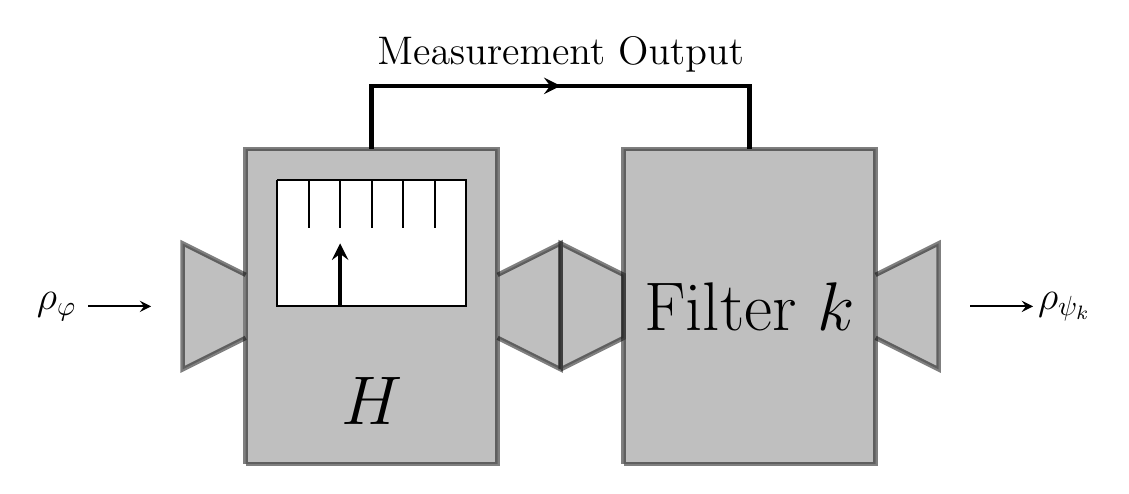
\begin{tikzpicture}[scale=0.8]
\draw[ultra thick,  fill=gray, opacity=0.5] (0,0) -- (4,0) -- (4,5) -- (0,5) -- (0,0);
\draw[ultra thick,  fill=gray, opacity=0.5] (0,2) -- (-1,1.5) -- (-1,3.5) -- (0,3);
\draw[ultra thick,  fill=gray, opacity=0.5] (4,2) -- (5,1.5) -- (5,3.5) -- (4,3);
\draw[thick, fill=white] (0.5,4.5) -- (3.5,4.5) -- (3.5,2.5) -- (0.5,2.5) -- (0.5,4.5);
\draw[thick] (1,4.5) -- (1,3.75);
\draw[thick] (1.5,4.5) -- (1.5,3.75);
\draw[thick] (2,4.5) -- (2,3.75);
\draw[thick] (2.5,4.5) -- (2.5,3.75);
\draw[thick] (3,4.5) -- (3,3.75);
\draw[ultra thick,->] (1.5,2.5) -- (1.5,3.5);
%%%%
\node at (2,1) {\Huge{$H$}};
\draw[thick, ->] (-2.5,2.5) -- (-1.5,2.5);
\node at (-3,2.5) {\Large{$\rho_{\varphi}$}};
%%%%%
\draw[ultra thick, fill=gray, opacity=0.5] (5,1.5) -- (6,2) -- (6,3) -- (5,3.5) -- (5,1.5); 
\draw[ultra thick, fill=gray, opacity=0.5] (6,0) -- (10,0) -- (10,5) -- (6,5) -- (6,0);
\draw[ultra thick, fill=gray, opacity=0.5] (10,2) -- (11,1.5) -- (11,3.5) -- (10,3);
\node at (8,2.5) {\Huge{Filter $k$}};
\draw[thick, ->] (11.5,2.5) -- (12.5,2.5);
\node at (13,2.5) {\Large{$\rho_{\psi_k}$}};
%%%%%
\draw[ultra thick] (4.5,6) -- (8,6) -- (8,5);
\draw[ultra thick,->] (2,5) -- (2,6) -- (5,6);
\node at (5,6.5) {\Large{Measurement Output}};
\end{tikzpicture}
\end{center}

We feed in a general pure state of our system into the $H$ device, which measures the energy of that pure state. It then sends this measurement output into the filter device. The state post measurement is then fed into the filter device, which is designed to only let something pass through it if the measurement was $E_k$. In this way the \emph{only} pure state that can leave is $\rho_{\psi_k}$. 

Note, although the final output is guaranteed to be $\rho_{\psi_k}$, that does not mean that the output from the $H$ device is always $\rho_{\psi_k}$ --- it could be \emph{any} of the possible output states. It is also important that $H$ is non-degenerate, otherwise the filter would let multiple different states through, all of which gave $E_k$ as their measurement output. 

For (ii) we allow for degeneracy of $H$. We overcome this by considering a \emph{maximal set of mutually commuting observables}, $\{A_1,...,A_f\}$, for which there are common eigenvectors $\psi_{a_1,...,a_f}$ with \bse 
A_i \psi_{a_1,...,a_f} = a_i \psi_{a_1,...,a_f}.
\ese 
The maximal set means that these states are uniquely determined using these operators; that is we have a subset of eigenvectors which we differentiate using this maximal set of commuting operators. The device looks like 
\begin{center}
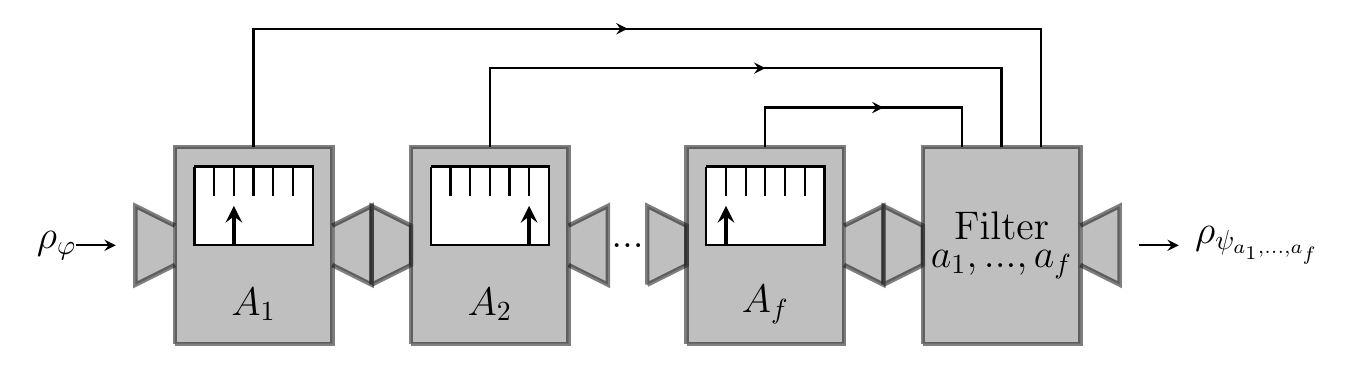
\begin{tikzpicture}[scale=0.5]
\draw[ultra thick,  fill=gray, opacity=0.5] (0,0) -- (4,0) -- (4,5) -- (0,5) -- (0,0);
\draw[ultra thick,  fill=gray, opacity=0.5] (0,2) -- (-1,1.5) -- (-1,3.5) -- (0,3);
\draw[ultra thick,  fill=gray, opacity=0.5] (4,2) -- (5,1.5) -- (5,3.5) -- (4,3);
\draw[thick, fill=white] (0.5,4.5) -- (3.5,4.5) -- (3.5,2.5) -- (0.5,2.5) -- (0.5,4.5);
\draw[thick] (1,4.5) -- (1,3.75);
\draw[thick] (1.5,4.5) -- (1.5,3.75);
\draw[thick] (2,4.5) -- (2,3.75);
\draw[thick] (2.5,4.5) -- (2.5,3.75);
\draw[thick] (3,4.5) -- (3,3.75);
\draw[ultra thick,->] (1.5,2.5) -- (1.5,3.5);
%%%%
\node at (2,1) {\Large{$A_1$}};
\draw[thick, ->] (-2.5,2.5) -- (-1.5,2.5);
\node at (-3,2.5) {\Large{$\rho_{\varphi}$}};
%%%%%
\draw[ultra thick, fill=gray, opacity=0.5] (5,1.5) -- (6,2) -- (6,3) -- (5,3.5) -- (5,1.5); 
\draw[ultra thick, fill=gray, opacity=0.5] (6,0) -- (10,0) -- (10,5) -- (6,5) -- (6,0);
\draw[ultra thick, fill=gray, opacity=0.5] (10,2) -- (11,1.5) -- (11,3.5) -- (10,3);
\draw[thick, fill=white] (6.5,4.5) -- (9.5,4.5) -- (9.5,2.5) -- (6.5,2.5) -- (6.5,4.5);
\draw[thick] (7,4.5) -- (7,3.75);
\draw[thick] (7.5,4.5) -- (7.5,3.75);
\draw[thick] (8,4.5) -- (8,3.75);
\draw[thick] (8.5,4.5) -- (8.5,3.75);
\draw[thick] (9,4.5) -- (9,3.75);
\draw[ultra thick,->] (9,2.5) -- (9,3.5);
\node at (8,1) {\Large{$A_2$}};
\node at (11.5,2.5) {\Large{...}};
%%%%%
\draw[ultra thick, fill=gray, opacity=0.5] (12,1.5) -- (13,2) -- (13,3) -- (12,3.5) -- (12,1.5); 
\draw[ultra thick, fill=gray, opacity=0.5] (13,0) -- (17,0) -- (17,5) -- (13,5) -- (13,0);
\draw[ultra thick, fill=gray, opacity=0.5] (17,2) -- (18,1.5) -- (18,3.5) -- (17,3);
\draw[thick, fill=white] (13.5,4.5) -- (16.5,4.5) -- (16.5,2.5) -- (13.5,2.5) -- (13.5,4.5);
\draw[thick] (14,4.5) -- (14,3.75);
\draw[thick] (14.5,4.5) -- (14.5,3.75);
\draw[thick] (15,4.5) -- (15,3.75);
\draw[thick] (15.5,4.5) -- (15.5,3.75);
\draw[thick] (16,4.5) -- (16,3.75);
\draw[ultra thick,->] (14,2.5) -- (14,3.5);
\node at (15,1) {\Large{$A_f$}};
%%%%
\draw[ultra thick, fill=gray, opacity=0.5] (18,1.5) -- (19,2) -- (19,3) -- (18,3.5) -- (18,1.5); 
\draw[ultra thick, fill=gray, opacity=0.5] (19,0) -- (23,0) -- (23,5) -- (19,5) -- (19,0);
\draw[ultra thick, fill=gray, opacity=0.5] (23,2) -- (24,1.5) -- (24,3.5) -- (23,3);
\node at (21,3) {\Large{Filter}};
\node at (21,2) {\Large{$a_1,...,a_f$}};
%%%%%
\draw[thick, ->] (24.5,2.5) -- (25.5,2.5);
\node at (27.5,2.5) {\Large{$\rho_{\psi_{a_1,...,a_f}}$}};
%%%%%
\draw[thick, ->] (2,5) -- (2,8) -- (11.5,8); 
\draw[thick] (11,8) -- (22,8) -- (22,5);
\draw[thick, ->] (8,5) -- (8,7) -- (15,7); 
\draw[thick] (14.5,7) -- (21,7) -- (21,5);
\draw[thick, ->] (15,5) -- (15,6) -- (18,6); 
\draw[thick] (17.5,6) -- (20,6) -- (20,5);
\end{tikzpicture}
\end{center}

\subsection{Mixed States}
Mixed states encode the `ignorance' (in the sense of lack of knowledge) on behalf of the experimenter/equipment. For example, the experimenter's inability to see exactly where the pointer is pointing, and so takes a guess at the reading. This introduces further uncertainty into which final state we obtain. It is important to note, though, that this is \emph{not} and inherently quantum mechanical property. 

The typical set up for preparing a mixed state is as follows: 

\begin{center}
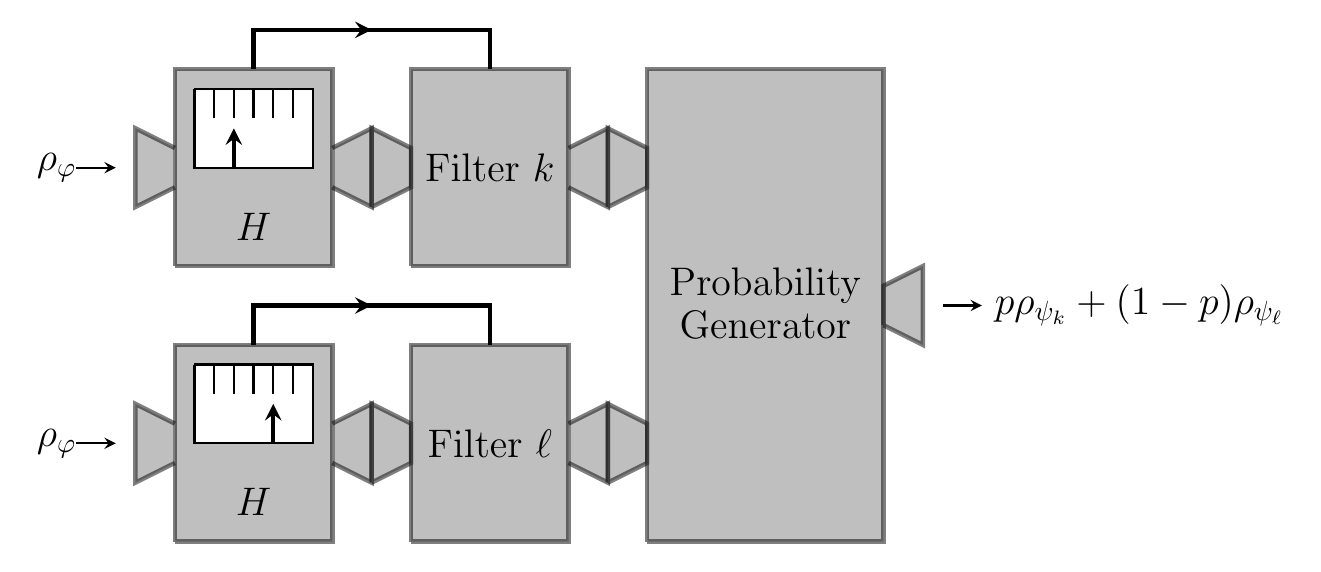
\begin{tikzpicture}[scale=0.5]
\draw[ultra thick,  fill=gray, opacity=0.5] (0,7) -- (4,7) -- (4,12) -- (0,12) -- (0,7);
\draw[ultra thick,  fill=gray, opacity=0.5] (0,9) -- (-1,8.5) -- (-1,10.5) -- (0,10);
\draw[ultra thick,  fill=gray, opacity=0.5] (4,9) -- (5,8.5) -- (5,10.5) -- (4,10);
\draw[thick, fill=white] (0.5,11.5) -- (3.5,11.5) -- (3.5,9.5) -- (0.5,9.5) -- (0.5,11.5);
\draw[thick] (1,11.5) -- (1,10.75);
\draw[thick] (1.5,11.5) -- (1.5,10.75);
\draw[thick] (2,11.5) -- (2,10.75);
\draw[thick] (2.5,11.5) -- (2.5,10.75);
\draw[thick] (3,11.5) -- (3,10.75);
\draw[ultra thick,->] (1.5,9.5) -- (1.5,10.5);
\node at (2,8) {\Large{$H$}};
\draw[thick, ->] (-2.5,9.5) -- (-1.5,9.5);
\node at (-3,9.5) {\Large{$\rho_{\varphi}$}};
\draw[ultra thick, fill=gray, opacity=0.5] (5,8.5) -- (6,9) -- (6,10) -- (5,10.5) -- (5,8.5); 
\draw[ultra thick, fill=gray, opacity=0.5] (6,7) -- (10,7) -- (10,12) -- (6,12) -- (6,7);
\draw[ultra thick, fill=gray, opacity=0.5] (10,9) -- (11,8.5) -- (11,10.5) -- (10,10);
\node at (8,9.5) {\Large{Filter $k$}};
\draw[ultra thick] (4.5,13) -- (8,13) -- (8,12);
\draw[ultra thick,->] (2,12) -- (2,13) -- (5,13);
%%%%%%%%%%%%
\draw[ultra thick,  fill=gray, opacity=0.5] (0,0) -- (4,0) -- (4,5) -- (0,5) -- (0,0);
\draw[ultra thick,  fill=gray, opacity=0.5] (0,2) -- (-1,1.5) -- (-1,3.5) -- (0,3);
\draw[ultra thick,  fill=gray, opacity=0.5] (4,2) -- (5,1.5) -- (5,3.5) -- (4,3);
\draw[thick, fill=white] (0.5,4.5) -- (3.5,4.5) -- (3.5,2.5) -- (0.5,2.5) -- (0.5,4.5);
\draw[thick] (1,4.5) -- (1,3.75);
\draw[thick] (1.5,4.5) -- (1.5,3.75);
\draw[thick] (2,4.5) -- (2,3.75);
\draw[thick] (2.5,4.5) -- (2.5,3.75);
\draw[thick] (3,4.5) -- (3,3.75);
\draw[ultra thick,->] (2.5,2.5) -- (2.5,3.5);
\node at (2,1) {\Large{$H$}};
\draw[thick, ->] (-2.5,2.5) -- (-1.5,2.5);
\node at (-3,2.5) {\Large{$\rho_{\varphi}$}};
\draw[ultra thick, fill=gray, opacity=0.5] (5,1.5) -- (6,2) -- (6,3) -- (5,3.5) -- (5,1.5); 
\draw[ultra thick, fill=gray, opacity=0.5] (6,0) -- (10,0) -- (10,5) -- (6,5) -- (6,0);
\draw[ultra thick, fill=gray, opacity=0.5] (10,2) -- (11,1.5) -- (11,3.5) -- (10,3);
\node at (8,2.5) {\Large{Filter $\ell$}};
\draw[ultra thick] (4.5,6) -- (8,6) -- (8,5);
\draw[ultra thick,->] (2,5) -- (2,6) -- (5,6);
%%%%%%%%%%
\draw[ultra thick, fill=gray, opacity=0.5] (11,1.5) -- (12,2) -- (12,3) -- (11,3.5) -- (11,1.5);
\draw[ultra thick, fill=gray, opacity=0.5] (11,8.5) -- (12,9) -- (12,10) -- (11,10.5) -- (11,8.5);
\draw[ultra thick, fill=gray, opacity=0.5] (12,0) -- (18,0) -- (18,12) -- (12,12) -- (12,0);
\draw[ultra thick, fill=gray, opacity=0.5] (18,5.5) -- (18,6.5) -- (19,7) -- (19,5) -- (18,5.5);
\node at (15,6.5) {\Large{Probability}};
\node at (15,5.5) {\Large{Generator}};
\draw[thick, ->] (19.5,6) -- (20.5,6);
\node at (24.5,6) {\Large{$p\rho_{\psi_k}+(1-p)\rho_{\psi_{\ell}}$}};
\end{tikzpicture}
\end{center}

The `probability' generator here is some method of choosing which input (left) to output (right), where there is a probability $p$ to use the top input ($\psi_k$). For example it could be a person rolling a dice that says "If I roll a `1' then I shall use the top input, otherwise I'll use the bottom one," in which case $p=1/6$. Normalisation is taken care of by requiring the other possible outcome to have probability $(1-p)$. 

\br 
It is very important to realise the the output for a mixed state is the sum of two \emph{states}; it is not the state made from the sum of two eigenvectors, as was the case with \Cref{ex:PureStatePreparationLinearCombination}. That is 
\bse 
p\rho_{\psi_k} + (1-p)\rho_{(1-p)\psi_{\ell}} \neq \rho_{p\psi_k + (1-p)\psi_{\ell}}.
\ese 
We highlight this point here as it demonstrates one of the misleading aspects of using bra-ket notation. People often talk about a pure state as one that can be written as a linear superposition of the eigenstates (as with \Cref{ex:PureStatePreparationLinearCombination}), writing 
\bse
\textcolor{blue}{\ket{\Psi} = a\ket{\psi_k} + b\ket{\psi_{\ell}} },
\ese 
for $a,b\in\C$ and $k\neq \ell$, where the normalisation condition requires $|a|^2+|b|^2=1$. But if were to think of \textcolor{blue}{$\ket{\Psi}$} as the \emph{state} then this would look like a mixed state --- it is the superposition of two pure \emph{states}. 

In order to differentiate a pure state from a mixed state they introduce the density matrices, which are the $\rho$s we've been using, and say that the density matrix of a mixed state is of the form 
\bse 
\textcolor{blue}{ \rho_{\text{mixed}} = \sum_i p_i \ket{\psi_i}\bra{\psi_i} },
\ese 
where $p_i$ is the probability of being in the corresponding state, but then going back to the start of section 17.3, we see this is just the same as what we wrote for a mixed state, without any of the potential confusion. 
\er 
\newpage

\section{The Fourier Operator}
This lecture will begin our systematic approach to the study of the so-called \emph{Sch\"{o}dinger operator}:
\bse 
H : \cD_H \to L^2(\R^d),
\ese 
with 
\bse 
(H\psi)(x) := -\frac{\hbar^2}{2m}(\Laplace \psi)(x) + V(x)\psi(x),
\ese 
where $\Laplace := \partial_1^2+...+\partial_d^2$ is the \emph{Laplacian operator} and $V(x)$ is the potential. The \emph{Fourier operator} is an indispensable toll in conducting the study. 

We will start by expanding on \Cref{lem:SchwartzSpaceFourierIsomorphism}. We will then use the fact that the Schwartz space is densely defined on $L^2(\R^d)$ along with the BLT theorem to provide a proscription for taking the Fourier transform on $L^2(\R^d)$.

\subsection{The Fourier Operator on Schwartz Space}

Recalling the definition of the Schwartz space, it is clear that the following facts hold: If $f\in S(\R^d)$ then 
\ben[label=(\roman*)]
\item $Q^kf\in S(\R^d)$ for all $k=1,...,d$, where $Q^k$ is the $k$-th position operator. 
\item $P_kf\in S(\R^d)$ for all $k=1,...,d$, where $P_k$ is the $k$-th momentum operator. 
\een 
We shall use these facts in the following calculations. 

\bd 
The \emph{Fourier operator} on Schwartz space is the linear map $\fF:S(\R^d) \to S(\R^d)$ with 
\bse
(\fF f)(x) := \frac{1}{(2\pi)^{d/2}} \int_{\R^d} d^dy e^{-ixy} f(y),
\ese 
where $xy := x_1y_1 + ... + x_dy_d$.
\ed 

\br 
We are using the $1/(2\pi)^{d/2}$ convention in the definition above. As we shall see, all that is required is a `total of' $1/(2\pi)$ between the Fourier operator and it's inverse. This convention is often used as it makes comparing to the inverse easier. Other conventions (for example having $1/(2\pi)$ appear in the inverse and just have unit coefficient in the above) find use in certain cases (for example if you were only concerned with taking $\fF$).
\er 

\br 
We shall also called the action of the Fourier operator on a function $f\in S(\R^d)$ the Fourier \emph{transform} of the function. 
\er 

We now wish to make some remarks on notation. 
\ben[label=(\roman*)]
\item Particularly in physics, it is often intuitive to think of $f$ as a function on `position space' (in the sense that its argument is a position space), while thinking of the Fourier transform $\fF f $ as a function on momentum space. Thus, one often relabels the variables as follows 
\bse 
(\fF f)(p) := \frac{1}{(2\pi)^{d/2}} \int_{\R^d} d^dy e^{-ipx} f(x).
\ese 

While this does have its advantages at times (the famous example being the motivation behind the derivation of Heisenberg's uncertainty relation, a truly vital relation in quantum mechanics), it can also lead to misconceptions. For example, when thought of this way, one may think that you can not take the double Fourier transform $\fF(\fF f)$, as the first one gives a momentum space, which the second does not `act on'. However from the definition given, this is clearly nonsense --- of course you can take it twice as $\fF : S(\R^d) \to S(\R^d)$. 

We shall, however, stick to this notation, but we should not be fooled by what we can take the Fourier transform of because of it.
\item Recall that $(Q^kf)(x)= x^k f(x)$ which is just a real number. It is therefore totally meaningless to write something of the form 
\bse 
\fF \big(x^kf(x)\big).
\ese 
However having to define the operators each time and then taking the Fourier transform of their action on a function could end up quite lengthy, so instead we introduce the following notations 
\bse 
\reallywidehat{x^kf(x)} := \fF (Q^kf),
\ese 
and 
\bse 
\fF \big(x\mapsto x^kf(x)\big),
\ese  
and similarly for other operators. 

The former of these two is how one usually sees the Fourier transform written, and it often just written as 
\bse 
\reallywidehat{g} := \fF g,
\ese 
where $g$ is the result of the action of the operator on $f$ (so here $g:= Q^kf$).
\een 

\bp 
\label{prop:FourierDerivatives}
Let $f\in S(\R^d)$ and $\gamma\in\N_0^d$. Then 
\ben[label=(\roman*)]
\item $\fF\big((-i)^{|\gamma|} \partial_{\gamma}f\big)(p) = p_{\gamma} \cdot \big(\fF f\big)(p)$. 
\item $\fF\big(x\mapsto x^{\gamma}f\big)(p) = i^{|\gamma|}\big[\partial_{\gamma}\big(\fF f\big)\big](p)$.
\een 
\ep 

\bq 
We shall prove these both by induction. 
\ben[label=(\roman*)]
\item Let $\gamma=k$, and so $|\gamma|=1$. Then, using integration by parts, we have
\bi{rCl}
\fF \big(-i\partial_kf)(p) & := & \frac{1}{(2\pi)^{d/2}} \int_{\R^d} d^dx e^{-ipx} (-i)\big(\partial_kf\big)(x) \\
& = & -\frac{1}{(2\pi)^{d/2}} \int_{\R^d} d^dx (-ip_k)e^{-ipx} (-i)f(x) + \bigg[ \frac{-i}{(2\pi)^{d/2}} e^{-ipx} f(x) \bigg]_{\partial \R^d} \\
& = & p_k \cdot \frac{1}{(2\pi)^{d/2}} \int_{\R^d} d^dx e^{-ipx}f(x) \\
& = & p_k \cdot \big(\fF f\big)(p),
\ei 
where we have used the fact that the elements of the Schwartz space are rapidly decaying to remove the boundary term. 

Now assume it is true for $|\gamma| = n$. Then, if $\gamma'$ is the next step, from the fact that $\partial_k f\in S(\R^d)$ we have 
\bi{rCl}
\fF \big((-i)^{n+1} \partial_{\gamma_1}\partial_{\gamma_2}...\partial_{\gamma_{n+1}} f\big) (p) & = & \fF \big( (-i)^n \partial_{\gamma_1}\partial_{\gamma_2}...\partial_{\gamma_n}(-i\partial_{\gamma_{n+1}}f)\big)(p) \\
& = & p_{\gamma_1}p_{\gamma_2}...p_{\gamma_n} \cdot  \fF\big(-i\partial_{\gamma_{n+1}}f\big)(p) \\
& = & p_{\gamma_1}...p_{\gamma_n}p_{\gamma_{n+1}}\cdot \big(\fF f\big)(p) \\
& =: & p_{\gamma'}\cdot \big(\fF f\big)(p) 
\ei 
\item Again let $\gamma=k$, then
\bi{rCl}
\fF\big(x\mapsto x^kf(x)\big)(p) & := & \frac{1}{(2\pi)^{d/2}}\int_{\R^d}d^dx e^{ipx}x^kf(x) \\
& = & \frac{1}{(2\pi)^{d/2}} \int_{\R^d}d^d i\frac{\partial}{\partial p^k} \big(e^{-ipx}\big)f(x) \\
& = & i\frac{\partial}{\partial p^k} \bigg[ \frac{1}{(2\pi)^{d/2}} \int_{\R^d}d^dx e^{-ipx}f(x) \bigg] \\
& =: & i \bigg(\frac{\partial}{\partial p^k} \fF f\bigg)(p).
\ei 
Then using the notation $\partial_k$ gives the result here. In fact, we should have really written $\partial_k(p\mapsto e^{-ipx})$ on the second line --- i.e. you take the derivative before you evaluate at $x$. 
Now assume its true for $|\gamma|=n$. Then,  if $\gamma'$ is the next step, we have 
\bi{rCl}
\fF\big(x\mapsto x^{\gamma_1}...x^{\gamma_{n+1}}f(x)\big)(p) & = & \fF\Big(x\mapsto x^{\gamma_1}...x^{\gamma_n}\big(y\mapsto y^{\gamma_{n+1}}f(y)\big)\Big)(p) \\
& = & i^n \big[\partial_{\gamma_1}...\partial_{\gamma_n}\fF\big(y\mapsto y^{\gamma_{n+1}}f(y)\big)\big](p) \\
& = & i^{n+1} \big[\partial_{\gamma'}(\fF f)\big](p)
\ei 
\een 
\eq 

\bp 
Let $f\in S(\R^d)$. 
\ben[label=(\roman*)]
\item Let $a\in\R^d$, then
\bse 
\reallywidehat{f(x-a)}(p) = e^{iap} \cdot \reallywidehat{f(x)}(p).
\ese 
\item Let $\lambda\in\C$, then 
\bse 
\reallywidehat{f(\lambda x)}(p) = \frac{1}{\lambda^d}\reallywidehat{f(x)}\bigg(\frac{p}{\lambda}\bigg).
\ese 
\een 
\ep 

\bq 
\ben[label=(\roman*)]
\item Using the change of variables $y=x-a$, we have 
\bi{rCl}
\reallywidehat{f(x-a)}(p) & := & \frac{1}{(2\pi)^{d/2}}\int_{\R^d} d^dx e^{-ipx}f(x-a) \\
& = & \frac{1}{(2\pi)^{d/2}}\int_{\R^d} d^dy e^{-ip(y+a))}f(y) \\
& = & e^{-ipa} \cdot \frac{1}{(2\pi)^{d/2}}\int_{\R^d} d^dx e^{-ipx}f(x) \\
& =: & e^{-ipa} \reallywidehat{f(x)}(p),
\ei 
where we relabelled $y\to x$ again. 
\item Using the change of variables $y=\lambda x$
\bi{rCl}
\reallywidehat{f(\lambda x)}(p) & = & \frac{1}{(2\pi)^{d/2}} \int_{\R^d} d^dx e^{-ipx}f(\lambda x) \\
& = &  \frac{1}{(2\pi)^{d/2}} \int_{\R^d} \frac{1}{\lambda^d} d^dy e^{-ip\frac{y}{\lambda}} f(y) \\
& = & \frac{1}{\lambda^d}\frac{1}{(2\pi)^{d/2}} \int_{\R^d} d^dx e^{-i\frac{p}{\lambda} x} f(x) \\
& = & \frac{1}{\lambda^d}\reallywidehat{f(x)}\bigg(\frac{p}{\lambda}\bigg),
\ei 
where again we relabelled $y\to x$.
\een 
\eq 

\subsection{Inverse of Fourier Operator}

\br 
This is often also called `the inverse Fourier transform'.
\er 

\bl 
\label{lem:FourierExponentialSquare}
Let $x\in\R^d$ and $z\in\C$ with $\Re(z)>0$. Then the following is true.
\bse 
\reallywidehat{\exp\Big(-\frac{z}{2}x^2\Big)}(p) = \frac{1}{z^{d/2}} \exp\Big(-\frac{1}{2z}p^2\Big).
\ese 
\el 

\bq 
We shall prove this for the case $d=1$. Let 
\bse 
G_z(x) := \exp\Big(-\frac{z}{2}x^2\Big).
\ese 
Then we have 
\bi{rCl}
\big(\partial G_z\big)(x) & = & -zx G_z(x) \\
ip\cdot \big(\fF G_z\big)(p) & = & -iz \big[ \partial\big(\fF G_z\big) \big] (p),
\ei 
which is an ODE for $\fF G_z$. Solving by separation (as done when considering the quantum harmonic oscillator) we arrive at 
\bse 
\big(\fF G_z\big)(p) = A \exp\Big(-\frac{p^2}{2z}\Big).
\ese 
Plugging in $p=0$ and the definitions for the LHS gives 
\bse 
\frac{1}{\sqrt{2\pi}} \int_{\R} dx 1 \cdot  e^{-\frac{z}{2}x^2} = A.
\ese 
Then employing the fact that the integral above is holomorphic\footnote{See `Fourier Series, Fourier Transform and Their Application to Mathematical Physics' by V. Serov Capter 16} we we extend the standard integral result 
\bse 
\int_{\R} dx e^{-i\sigma x^2} = \sqrt{\frac{\pi}{\sigma}},
\ese 
for $\sigma\in\R$ to the case we are considering, giving
\bse 
A = \frac{1}{\sqrt{z}}.
\ese 
\eq 

\bt 
The Fourier operator $\fF : S(\R^d)\to S(\R^d)$ is invertable with inverse 
\bse 
\big(\fF^{-1}g\big)(x) = \frac{1}{(2\pi)^{d/2}} \int_{\R^d} d^dp e^{+ipx}g(p).
\ese 
\et 

\bq 
Need to show that $\big[\fF^{-1}\big(\fF f\big)\big](x) = f(x)$. In order to do so, we shall have to introduce a regulator
\bse 
\lim_{\varepsilon\to0} e^{-\frac{\varepsilon}{2}p^2} = 1
\ese 
into the integral. We shall then use the fact that $\big(\fF f\big)(p)$ will be dominant and the fact that we are using Lebesgue integrals to pull out the limit. We shall also use Fubini's theorem to move the order of the integrals.
\bi{rCl}
\big[\fF^{-1}\big(\fF f\big)\big](x) & := & \frac{1}{(2\pi)^{d/2}} \int_{\R^d} d^dp e^{ipx}\big(\fF f\big)(p) \\
& = & \frac{1}{(2\pi)^{d/2}} \int_{\R^d} d^dp \lim_{\varepsilon\to0} e^{-\frac{\varepsilon}{2}p^2} e^{ipx}\big(\fF f\big)(p) \\
& = & \lim_{\varepsilon\to0}\frac{1}{(2\pi)^{d/2}} \int_{\R^d} d^dp  e^{-\frac{\varepsilon}{2}p^2} e^{ipx}\big(\fF f\big)(p) \\
& := & \lim_{\varepsilon\to0}\frac{1}{(2\pi)^{d/2}} \int_{\R^d} d^dp  e^{-\frac{\varepsilon}{2}p^2} e^{ipx} \frac{1}{(2\pi)^{d/2}}\int_{\R^d}d^dy e^{-ipy} f(y) \\
& = & \lim_{\varepsilon\to0}\frac{1}{(2\pi)^{d/2}}\int_{\R^d}d^dy \frac{1}{(2\pi)^{d/2}} \int_{\R^d} d^dp  e^{-\frac{\varepsilon}{2}p^2} e^{ipx}  e^{-ipy} f(y) \\
& = & \lim_{\varepsilon\to0}\frac{1}{(2\pi)^{d/2}}\int_{\R^d}d^dy \frac{1}{(2\pi)^{d/2}} \int_{\R^d} d^dp  e^{-\frac{\varepsilon}{2}p^2} e^{-ip(y-x)} f(y) \\
& = & \lim_{\varepsilon\to0}\frac{1}{(2\pi)^{d/2}}\int_{\R^d}d^dy \frac{1}{(2\pi)^{d/2}} \int_{\R^d} d^dp  e^{-\frac{\varepsilon}{2}p^2} e^{ipx}  e^{-ipy} f(y) \\
& = & \lim_{\varepsilon\to0}\frac{1}{(2\pi)^{d/2}}\int_{\R^d}d^dz \frac{1}{(2\pi)^{d/2}} \int_{\R^d} d^dp  e^{-\frac{\varepsilon}{2}p^2} e^{-ipz} f(z+x) \\
& = & \lim_{\varepsilon\to0}\frac{1}{(2\pi)^{d/2}}\int_{\R^d}d^dz \bigg[\reallywidehat{\exp\Big(-\frac{\varepsilon}{2}p^2\Big)}(z)\bigg] f(z+x) \\
& = & \lim_{\varepsilon\to0}\frac{1}{(2\pi)^{d/2}}\int_{\R^d}d^dz \frac{1}{\varepsilon^{d/2}} \exp \Big(-\frac{1}{2\varepsilon}z^2\Big) f(z+x) \\
& = & \lim_{\varepsilon\to0}\frac{1}{(2\pi)^{d/2}}\int_{\R^d}d^dz' \varepsilon^{d/2} \frac{1}{\varepsilon^{d/2}} \exp \Big(-\frac{1}{2\varepsilon}\big(\varepsilon z'\big)^2\Big) f\big(\sqrt{\varepsilon}z'+x\big) \\
& = & \frac{1}{(2\pi)^{d/2}}\int_{\R^d} d^dz' \exp\Big(-\frac{1}{2}\big(z'\big)^2\Big) \lim_{\varepsilon\to0} f\big(\sqrt{\varepsilon}z' +x\big) \\
& = & \frac{1}{(2\pi)^{d/2}} (2\pi)^{d/2}f(x) \\
& = & f(x),
\ei 
where we have used the substitutions $z=y+x$ and then $z = \sqrt{\varepsilon}z'$ along with the standard integral result used in the previous lemma.
\eq 

\subsection{Extension of $\fF$ to $L^2(\R^d)$}

We already know that $\fF$ is densely defined on $L^2(\R^2)$, so if we can show it is bounded the BLT theorem will tell us there is a unique, bounded extension of $\fF$ on $L^2(\R^d)$. 

\bt[Parseval's Theorem]
Let $f\in S(\R^d)$, then
\bse 
\int_{\R^d}d^dp \big| \big(\fF f\big)(p)\big|^2 = \int_{\R^d} d^dx |f(x)|^2.
\ese 
\et 

\bq 
The proof follows by direct calculation. 
\bi{rCl}
\int_{\R^d}d^dp \big| \big(\fF f\big)(p)\big|^2 & = & \int_{\R^d}d^dp \bigg| \int_{\R^d}d^dxe^{-ipx}f(x) \bigg|^2 \\
& = & \int_{\R^d}d^dp \int_{\R^d}d^dx\Big|e^{-ipx} f(x) \Big|^2 \\
& = & \int_{\R^s}d^dp \int_{\R^d}d^dx |f(x)|^2 \\
& = & \int_{\R^d} d^dx |f(x)|^2,
\ei 
where we used the fact that the integral is over a real domain. 
\eq 

It follows from Parseval's theorem, then, that 
\bi{rCl}
\|\fF\| & := & \sup_{f\in S(\R^d)} \frac{\|\fF f\|^2_{S(\R^d)}}{\|f\|^2_{S(\R^d)}} \\
& = & \sup_{f\in S(\R^d)} \frac{ \sqrt{\int_{\R^d}d^dp\big|\big(\fF f\big)(p)\big|^2} }{\sqrt{\int_{\R^d} d^dx |f(x)|^2}} \\
& = & \sup_{f\in S(\R^d)} \sqrt{\frac{\int_{\R^d}d^dp \big| \big(\fF f\big)(p)\big|^2}{\int_{\R^d} d^dx |f(x)|^2}} \\
& = & 1,
\ei 
so we have a unique extension
\bse 
\fF : L^2(\R^2) \to L^2(\R^2).
\ese 

In practice if we wanted to take the Fourier transform of a function $f\in L^2(\R^d)\setminus S(\R^d)$ then we do it via the following prescription: Let $\{f_n\}_{n\in \N}\ss S(\R^d)$ with $\lim_{n\to\infty}f_n = f$, then 
\bse 
\fF f = \fF \Big(\lim_{n\to\infty} f_n\Big) = \lim_{n\to\infty} \big(\fF f_n\big),
\ese 
where we have used the fact that $\fF$ is bounded to remove the limit. 

\subsection{Convolutions}

\bd 
The \emph{convolution} of two functions $f,g\in L^1(\R^d)$, written $f * g$, is the $L^1(\R^d)$ function defined pointwise by 
\bse 
(f * g)(x) := \int_{\R^d}d^dyf(x-y)g(y).
\ese 
\ed 

\bl 
The convolution of two functions is symmetric, i.e. 
\bse 
f*g = g*f.
\ese 
\el 

\bq 
The result comes from simple change of variables along with the commutativity of the complex multiplication,
\bi{rCl}
(f * g)(x) & := & \int_{\R^d}d^dy \, f(x-y)g(y) \\
& = & (-1)^{2d} \int_{\R^d} d^dz \, f(z) g(x-z) \\
& = & \int_{\R^d} d^dz \, g(x-z) f(z) \\
& = & \int_{\R^d} d^dy \, g(x-y) f(y) \\ 
& =: & (g*f)(x),
\ei 
where the $(-1)^{2d}$ term comes from the fact that $dy=-dz$ along with the fact that the integral limits swap. Since $x\in\R^d$ was arbitrary, we have the result.
\eq 

\bl 
The convolution is associative, i.e. 
\bse 
(f*g)*h = f*(g*h).
\ese 
\el 

\bq 
By direct calculation using Fubini's Theorem, and the previous lemma:
\bi{rCl}
\big((f*g)*h\big)(x) & = & \big( h*(f*g)\big)(x) \\
& := & \int_{\R^d} d^dy \, h(x-y) (f*g)(x) \\
& = & \int_{\R^d} d^dy \, h(x-y) (g*f)(x) \\
& := & \int_{\R^s}d^dy \, h(x-y) \int_{\R^d} d^dz \, g(z-x) f(z) \\
& = & \int_{\R^d}d^du \int_{\R^d}d^dz \, h(u) g(z-u-y) f(z) \\
& = & \int_{\R^d}d^dz \bigg( \int_{\R^d}d^du \,  g(z-y-u)h(u)\bigg) f(z) \\
& = & \int_{\R^d}d^dz \, \big(g*h\big)(z-y) f(z) \\
& = & \int_{\R^d}d^dx \, \big(g*h\big)(x-y) f(x) \\
& = & \big((g*h)*f\big)(x) \\
& = & \big( f*(g*h)\big)(x),
\ei 
which holds for all $x\in\R^d$, giving the result.
\eq 

\bl 
The convolution is distributive across addition, i.e. 
\bse 
f*(g+h) = f*g + f*h,
\ese 
where the addition is defined pointwise. 
\el 

\bq 
This follows from the linearity of the Lebesgue integral:
\bi{rCl}
\big(f*(g+h)\big)(x) & := & \int_{\R^d}d^dy \, f(x-y) (g+h)(x) \\
& = & \int_{\R^d} \, f(x-y)g(x) + \int_{\R^d} \, f(x-y)h(x) \\
& = & (f*g)(x) + (f*h)(x),
\ei 
which holds for all $x\in\R^d$, giving the result. 
\eq 


\bt
\label{thrm:FourierConvolution}
The Fourier transform of the convolution of two functions is proportional to the product of their Fourier transforms, explicitly 
\bse 
\fF(f*g) = (2\pi)^{d/2} \fF(f)\cdot \fF(g).
\ese 
\et 

\bq 
By direct calculation, 
\bi{rCl}
\fF(f*g)(p) & := & \frac{1}{(2\pi)^{d/2}} \int_{\R^d} d^dx \,  e^{-ipx} (f*g)(x) \\
& := & \frac{1}{(2\pi)^{d/2}} \int_{\R^d} d^dx\, \bigg( e^{-ipx} \int_{\R^d}d^dy \, f(x-y)g(x) \bigg) \\
& = & \frac{1}{(2\pi)^{d/2}} \int_{\R^d}d^dz \bigg( e^{-ip(z+y)} \int_{\R^d} d^dy \, f(z) g(x) \bigg) \\
& = & \frac{1}{(2\pi)^{d/2}}\int_{\R^d}d^dz\int_{\R^d}d^dy \, e^{-ipz}f(z) e^{-ipy}g(y) \\
& = & (2\pi)^{d/2} \bigg(\frac{1}{(2\pi)^{2/pi}}\int_{\R^d}d^dz \, e^{ipz}f(z)\bigg) \cdot \bigg(\frac{1}{(2\pi)^{2/pi}}\int_{\R^d}d^dy \,  e^{ipy}g(y)\bigg) \\
& = & (2\pi)^{2/d} \big((\fF f)(p)\big)\cdot \big((\fF g)(p)\big),
\ei 
where we have used the fact that we can consider the convolution integration variable (the $y$) as a constant when relabelling the Fourier transform variable, and used the fact that the Fourier transform of a function is finite to make the integral of an integral into a product of integrals. Finally since this is true for all $p\in\R^d$ the result follows. 
\eq 
\newpage

\section{The Schrodinger Operator}
The Schr\"{o}dinger operator for a vanishing potential if given by
\bse 
\Hf := -\frac{\hbar^2}{2m} \Laplace
\ese 
and it corresponds to the energy observable for a free particle\footnote{Free particle here means what we think of classically as a free particle, it experiences no potential.} of mass $m$. 

This lecture aims to derive the spectrum of $\Hf$ and use it to study the time evolution of pure states. We shall consider $d=3$ throughout this lecture, and shall make use of the results of last lecture heavily. We shall also use units such that $m=\frac{1}{2}\hbar^2$ in order to lighten notation; i.e. $\Hf=-\Laplace$.

\subsection{Domain of Self Adjointness of $\Hf$}

If we want to talk about $\Hf$ being an observable, we need to show that it is self adjoint on some domain. From (i) in \Cref{prop:FourierDerivatives} it follows that 
\bse 
\fF(-\Laplace\psi)(p) = |p|^2 (\fF\psi)(p) =: (P^2\widehat{\psi})(p),
\ese 
where $|p|^2 := p_1^2+p_2^2+p_3^2$. In other words, 
\bse 
\fF(-\Laplace \psi) =: P^2\widehat{\psi}.
\ese 

\br 
The physicists says "in momentum space the Laplacian acts simply by multiplication of the norm of the momentum, $|p|^2$".
\er 

We can now rewrite the above by inserting $\id_{L^2(\R^3)}=\fF^{-1}\fF$ to give 
\bse 
\fF \circ \Hf \circ \fF^{-1}\circ \fF\psi = P^2 \circ \fF\psi ,
\ese 
from which is follows
\bse 
\fF\Hf\fF^{-1} = P^2,
\ese 
whose maximal domain is 
\bse 
\cD_{P^2} = \{\widehat{\psi}\in L^2(\R^3) \, | \, P^2 \widehat{\psi} \in L^2(\R^3) \}.
\ese 

\bt 
A maximally defined real multiplication operator is self adjoint on its maximal domain. 
\et 

\bq 
Let
\bi{rrCl}
A : & \cD_A & \to & \cH \\
& \psi & \mapsto & a\psi 
\ei 
where $a\in\R$ and $\cD$ is the maximal domain of $A$ (i.e. there are no elements outside this domain such that $a\psi\in\cH$). This operator is clearly symmetric as, for $\psi,\varphi\in\cD$
\bi{rCl}
\braket{\psi}{A\varphi} & = & \braket{\psi}{a\varphi} \\
& = & a\braket{\psi}{\varphi} \\
& = & \braket{\overline{a}\psi}{\varphi} \\
& = & \braket{a\psi}{\varphi} \\
& = & \braket{A\psi}{\varphi}.
\ei 
We have therefore $A\se A^*$, which means $\cD_A\se \cD_{A^*}$ with $A^*\psi=A\psi$ for all $\psi\in\cD_A$, but $\cD_A$ is maximal so there is no $\psi\notin \cD_A$ such that $A^*\psi=a\psi\in\cH$ and so $\cD_{A^*}\se \cD_A$. Therefore $A=A^*$ on this maximal domain.
\eq 

From this theorem, then, we have that $\fF\Hf\fF^{-1}$ is self adjoint on the domain $\cD_{P^2}$. 

\subsection{Spectrum of $\Hf$}

One can quickly find the spectrum of $\Hf$ using the resolvent map, 
\bse
R_{P^2} (z) = \frac{1}{|p|^2-z},
\ese 
from which is clearly follows that the resolvent set is simply 
\bse 
\rho(P^2) = \{z\in\C \, | \, z \neq |p|^2 \}. 
\ese 
Then using the fact that $|p|^2\in\R$ with $|p|^2 >0$\footnote{We use a strict equality as if $|p|^2 =0$ then there is no momentum and so the operator $P^2$ just maps it to 0.} we have 
\bse 
\rho(P^2) = \C\setminus\R^+_0.
\ese 
Then finally using the definition of the spectrum as the compliment of the resolvent set we get 
\bse 
\sigma(\Hf) = \sigma(P^2) = \R^+_0.
\ese 

\br 
This is not the method used in the lectures, which I\footnote{I being Richie} find more confusing. As I don't fully understand the latter parts of the proof provided (I think the main idea is introducing a form of the spectral theorem in which the integral is performed over the spectrum of the operator and then use the characteristic function Dr. Schuller introduced) I shall not type it up here to avoid potential confusion to the readers. If you do follow the complete method please feel free to contact me and I can add it and give you credit. 
\er 

\bp 
For every self adjoint operator there is always some transformation which transforms the operator into a mere multiplication operator.
\ep 

\br 
Once you know the transformation the self adjoint operator of interest, the spectrum always follows by the same method. 
\er 

\subsection{Time Evolution}

Recall that Axiom 4 tells us the evolution of a state is given by\footnote{We're using units such that $\hbar=1$.} 
\bse 
\rho_{\psi_{t_2}} = e^{-i(t_2-t_1)H} \rho_{\psi_{t_1}} e^{i(t-2-t_1)H},
\ese 
which for a pure state becomes 
\bse 
\frac{\braket{\psi_{t_2}}{\cdot}}{\braket{\psi_{t_2}}{\psi_{t_2}}}\psi_{t_2} = e^{-i(t_2-t_1)H} \frac{\braket{\psi_{t_1}}{\cdot}}{\braket{\psi_{t_1}}{\psi_{t_1}}}\psi_{t_1} e^{i(t_2-t_1)H}.
\ese 
If we now choose to view the RHS as the following composition 
\bse 
\frac{1}{\braket{\psi_{t_1}}{\psi_{t_2}}} \Big(e^{-i(t_2-t_1)H}\braket{\psi_{t_1}}{\cdot}\Big) \circ \Big( \psi_{t_1} e^{i(t_2-t_1)H}\Big) \textcolor{blue}{ = \frac{1}{\braket{\psi_{t_1}}{\psi_{t_2}}} \Big(e^{-i(t_2-t_1)H}\ket{\psi_{t_1}}\Big)\circ\Big(\bra{\psi_{t_1}}e^{i(t_2-t_1)H}\Big) },
\ese 
it follows that we can represent the time evolution of a pure \emph{state} via the evolution of the \emph{Hilbert space element} as
\bse  
\psi_{t_2} = e^{-i(t_2-t_1)H}\psi_{t_1}.
\ese  

\br 
We are assuming here that $H$ is time-independent. If it wasn't you would simply use an integral in the exponential.
\er 

\br 
We should note that in the above time is viewed as a parameter, not a coordinate --- i.e. this is \emph{not} a spacetime picture. The elements $\psi_{t_1}$ and $\psi_{t_2}$ are simply elements of the Hilbert space, each of which is associated to a different time. This can be compared to saying classically that the position of a particle is an element of $\R^3$, and at a later time its position is still an element of $\R^3$, although potentially a different one. 
\er 

Now for the free particle we have 
\bse 
\fF^{-1} P^2 \fF = \Hf,
\ese 
which, along with the fact that $P^2$ is a multiplicative operator, gives us 
\bse 
e^{-it\Hf} \fF^{-1} = \fF^{-1}e^{-itP^2}.
\ese 
Acting both sides on $\widehat{\psi}:= \fF\psi$ gives 
\bse 
e^{-it\Hf}\psi = \fF^{-1}\Big( p \mapsto e^{-it|p|^2} \cdot \widehat{\psi}(p) \Big),
\ese 
which a convolution of functions. It is then tempting to use use 
\bse 
f*g = (2\pi)^{d/2}\fF^{-1}\big((\fF f)\cdot (\fF g)\big)
\ese 
to give us\footnote{Remember $d=3$ here.} 
\bi{rCl}
e^{-it\Hf}\psi(x) = \frac{1}{(2\pi)^{3/2}} \Big(\fF^{-1}\big(p\mapsto e^{-it|p|^2}\big) * \psi\Big)(x),
\ei 
and then use \Cref{lem:FourierExponentialSquare} to give
\bse 
\fF^{-1}\big(p\mapsto e^{-it|p|^2}\big)(x) = \frac{1}{(2t)^{3/2}} e^{-\frac{1}{4it}|x|^2},
\ese 
however there is a problem with both of these steps. 

Firstly for us to use the convolution theorem we require both functions to be $L^1(\R^3)$. For $\psi$ we can simply take the intersection $\psi\in L^2(\R^3)\cap L^1(\R^3)$, however the exponential term is unavoidably not in $L^1(\R^3)$ (if you take the absolute value you get 1, and then integrating over all of $\R^3$ gives a divergent result). On top of that, in order to use \Cref{lem:FourierExponentialSquare} we require the real part of the coefficient to be strictly positive (in order to avoid the branch cut), but $\Re(it)=0$. 

Luckily we can fix both of these problems with the same step, regularisation. We regularise both by introducing a positive, real factor into the exponential and then taking the limit, 
\bse 
e^{-it|p|^2} = \lim_{\varepsilon\to0} e^{-(it+\varepsilon)|p|^2}.
\ese 
The addition of $\varepsilon$ stops the integral diverging (because of the minus sign) and we also have $\Re(it+\varepsilon) = \varepsilon >0$ and so we can use \Cref{lem:FourierExponentialSquare}.

So, using the continuity of the product and the inverse Fourier transform we have 
\bi{rCl}
e^{-it\Hf}\psi(x) & = & \bigg[\lim_{\varepsilon\to0} \bigg( x\mapsto \frac{1}{(2\pi)^{3/2}} \frac{1}{\big(2(it+\varepsilon)\big)^{3/2}} \exp\Big( -\frac{|x|^2}{4(it+\varepsilon)}\Big) \bigg)* \psi\bigg](x) \\
& := & \lim_{\varepsilon\to0} \frac{1}{\big(4\pi(it+\varepsilon)\big)^{3/2}} \int_{\R^3}d^3y \exp\bigg( -\frac{|x-y|^2}{4(it+\varepsilon)}\bigg) \psi(y).
\ei 
Finally using dominated convergence to take the limit inside the integral, we have\footnote{Note $t=t_2-t_1$ here.}
\bse 
\psi_{t_2}(x) = \frac{1}{(i4\pi t)^{3/2}} \int_{\R^3}d^3y \exp\bigg( - \frac{|x-y|^2}{i4t}\bigg) \psi_{t_1}(y).
\ese 

\subsection{Physical Interpretation (for the Patient Observer)}

After massaging the above result a bit we arrive at the famous `\emph{spreading of the wavefunction}' result.

First start by expanding 
\bse 
|x-y|^2 = |x|^2 + |y|^2 - 2xy
\ese 
to give 
\bse 
\psi_{t_2}(x) = \frac{\exp\Big( - \frac{|x|^2}{i4t}\Big)}{(i4\pi t)^{3/2}} \int_{\R^3} d^3y \exp\bigg( -i\frac{x}{2t} y\bigg) \exp\bigg( - \frac{|y|^2}{i4t}\bigg) \psi_{t_1}(y),
\ese 
which is a Fourier transform with result 
\bse 
\psi_{t_2}(x) = \frac{\exp\Big( - \frac{|x|^2}{i4t}\Big)}{(i2t)^{3/2}} \cdot \reallywidehat{\exp\Big( - \frac{|y|^2}{i4t}\Big) \psi_{t_1}(y)} \bigg(\frac{x}{2t}\bigg).
\ese 

We now use the fact that we have a patient observer (i.e. one who watches for a long time) to take the asymptotic behaviour\footnote{That is take the limit $t\to\infty$ at places where it wont cause problems.} to give 
\bse 
\psi_{t_2}(x) \sim \frac{\exp\Big( - \frac{|x|^2}{i4t}\Big)}{(i2t)^{3/2}} \widehat{\psi}_{t_1}\bigg(\frac{x}{2t}\bigg),
\ese 
which, if the $\psi$s were viewed as `waves' (i.e. plots on a graph) would indicate that the `wave spreads out over time'. In other words, simplifying to $\R$ instead of $\R^3$ we'd have something along the following diagram.
\begin{center}
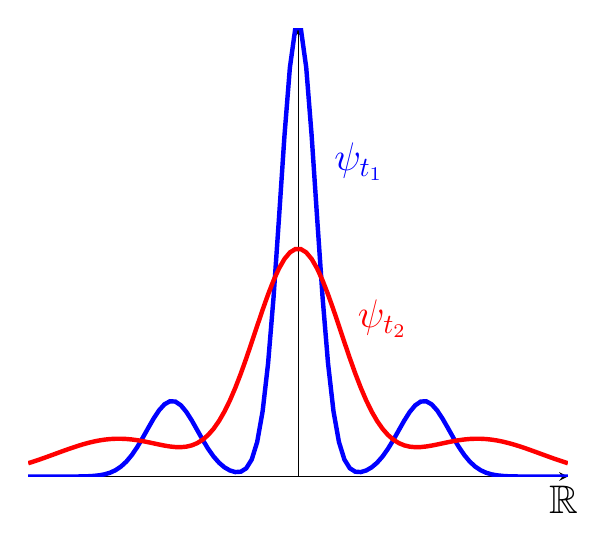
\begin{tikzpicture}
\begin{axis}[ticks=none,axis lines=middle]
    \addplot [domain=-15:15, samples=100, ultra thick, blue] {6*exp((-x*x)/2) + exp((-(x+7)^2)/4) +  exp((-(x-7)^2)/4)};
    \addplot [domain=-15:15, samples=100, ultra thick, red] {3*exp((-x*x)/12) + 0.5*exp((-(x+10)^2)/24) +  0.5*exp((-(x-10)^2)/24)};
\end{axis}
\node at (4.2,4) {\textcolor{blue}{\Large{$\psi_{t_1}$}}};
\node at (4.5,2) {\textcolor{red}{\Large{$\psi_{t_2}$}}};
\node at (6.8,-0.3) {\Large{$\R$}};
\end{tikzpicture}
\end{center}
So the function appears to spread out (keeping the area under it constant) over time. 
\newpage

\section{Periodic Potentials}
This lecture aims to look at periodic potentials and find the most general information we can about their energy spectrum. In order to do this we will use so-called \emph{Rigged Hilbert Spaces}.\footnote{I am currently reading up on these, and will add an additional section to the end of these notes once I have a better idea on them.}

\bd 
The Hamiltonian for a periodic potential is of the form 
\bse 
H = -\frac{\hbar^2}{2m} \Laplace + V(x),
\ese 
with 
\ben[label=(\roman*)]
\item Periodicity in $V(x)$, i.e. $V(x+a) = V(x)$ for all $x\in\R^3$ where $a$ is the periodicity of the system
\item $V$ is pointwise continuous and bounded.
\een 
\ed 

\begin{center}
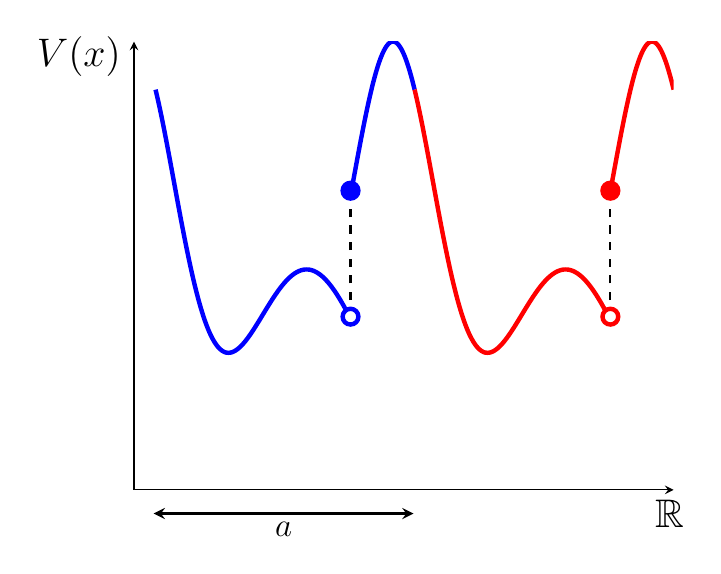
\begin{tikzpicture}
\begin{axis}[ticks=none,axis lines=middle]
    \addplot [domain=0.5:5, samples=100, ultra thick, blue] {6*exp((-x*x)/2) + 3*exp((-(x-4)^2)/4) + exp((-(x-10)^2)/6) + 3*exp((-(x+4)^2)/4) + exp((-(x+10)^2)/6)};
    \addplot [domain=5:6.5, samples=100, ultra thick, blue] {6*exp((-(x-6)^2)/2) + 3*exp((-(x-10)^2)/4) + exp((-(x-16)^2)/6) + 3*exp((-(x-2)^2)/4) + exp((-(x+4)^2)/6)};
    \addplot [domain=6.5:11, samples=100, ultra thick, red] {6*exp((-(x-6)^2)/2) + 3*exp((-(x-10)^2)/4) + exp((-(x-16)^2)/6) + 3*exp((-(x-2)^2)/4) + exp((-(x+4)^2)/6)};
    \addplot [domain=11:12.5, samples=100, ultra thick, red] {6*exp((-(x-12)^2)/2) + 3*exp((-(x-16)^2)/4) + exp((-(x-22)^2)/6) + 3*exp((-(x-8)^2)/4) + exp((-(x-2)^2)/6)};
    \addplot[domain=0:1]{0};
\end{axis}
\draw[dashed, thick] (2.75,2.2) -- (2.75,3.8);
\draw[blue, ultra thick, fill=white] (2.75,2.2) circle [radius=0.1];
\draw[blue, ultra thick, fill=blue] (2.75,3.8) circle [radius=0.1];
\draw[dashed, thick] (6.05,2.2) -- (6.05,3.8);
\draw[red, ultra thick, fill=white] (6.05,2.2) circle [radius=0.1];
\draw[red, ultra thick, fill=red] (6.05,3.8) circle [radius=0.1];
\node at (6.8,-0.3) {\Large{$\R$}};
\node at (-0.7,5.5) {\Large{$V(x)$}};
\draw[<->, thick] (0.25,-0.3) -- (3.55,-0.3);
\node at (1.9,-0.5) {\large{$a$}};
\end{tikzpicture}
\end{center}

As we shall see, by making no assumptions apart from the above, we will be able to extract a remarkable generic conclusion about the energy spectrum of particle moving in a generic periodic potential. This is truly a amazing result as the potential can even be discontinuous (countably) infinite times! A huge application of this formalism is in the study of solid state physics, where the periodic potential comes from that generated by a regular lattice of so-called \emph{lattice constant} $a$, 

\begin{center}
    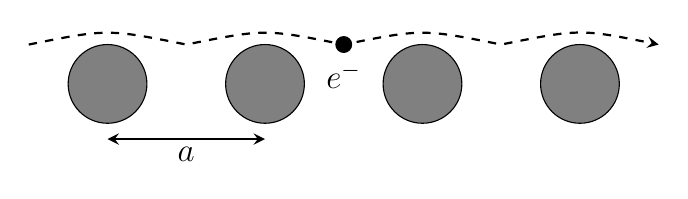
\begin{tikzpicture}
    \draw[fill=gray] (0,0) circle [radius=0.5];
    \draw[fill=gray] (2,0) circle [radius=0.5];
    \draw[fill=gray] (4,0) circle [radius=0.5];
    \draw[fill=gray] (6,0) circle [radius=0.5];
    \draw[<->, thick] (0,-0.7) -- (2,-0.7); 
    \node at (1,-0.9) {\large{$a$}};
    \draw[fill=black] (3,0.5) circle [radius=0.1];
    \node at (3,0.1) {\large{$e^-$}};
    \draw[->, thick, dashed] (-1, 0.5) .. controls (0,0.7) .. (1,0.5) .. controls (2,0.7) .. (3,0.5) .. controls (4,0.7) .. (5,0.5) .. controls (6,0.7) .. (7,0.5);
    \end{tikzpicture}
\end{center}

As we shall see the general result is that the energy spectrum comes in continuous, open intervals in $\R$, known as \emph{bands}.

\begin{center}
    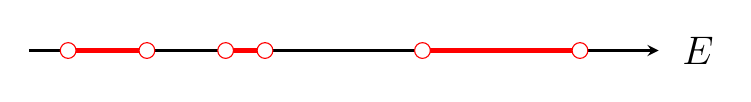
\begin{tikzpicture}
    \draw[thick, ->] (0,0) -- (8,0);
    \node at (8.5,0) {\Large{$E$}};
    \draw[ultra thick, red] (0.5,0) -- (1.5,0);
    \draw[red, fill=white] (0.5,0) circle [radius=0.1];
    \draw[red, fill=white] (1.5,0) circle [radius=0.1];
    \draw[ultra thick, red] (2.5,0) -- (3,0);
    \draw[red, fill=white] (2.5,0) circle [radius=0.1];
    \draw[red, fill=white] (3,0) circle [radius=0.1]; 
    \draw[ultra thick, red] (5,0) -- (7,0);
    \draw[red, fill=white] (5,0) circle [radius=0.1];
    \draw[red, fill=white] (7,0) circle [radius=0.1];
    \end{tikzpicture}
\end{center}

\subsection{Basics of Rigged Hilbert Space}

As mentioned at the start, we wish to make use of rigged Hilbert spaces\footnote{Again, coming soon!} in order to find the spectrum of the energy observable. The basic reason behind this is that rigged Hilbert spaces essentially extend what we usually think of as the eigenvalue equation
\bse 
H\psi = E\psi, 
\ese 
where $E$ is a discrete value in $\R$, to the case where $E$ can be continuous. This is known as the \emph{generalised eigenvalue equation}.

We do this because ultimately we know that the spectrum will be continuous intervals, however even if it was purely discrete, or a combination of both, the theory of rigged Hilbert spaces would still account for this. 

The basic idea behind rigged Hilbert spaces is to consider elements $\Psi$ that satisfy the generalised eigenvalue equation, but do not lie in $L^2(\R^d)$. It turns out that they lie in the adjoint of a densely defined subspace, which for us is the Schwartz space. In this way we construct our so-called \emph{Gelfand Triple}:
\bse 
S(\R^d) \ss L^2(\R^d) \ss S^*(\R^d).
\ese 

The easiest way to see that we need such a construction here is that, as the Hamiltonian is constructed using derivative operators, its eigenvalues are likely to be of the form 
\bse 
\Psi \propto e^{iE},
\ese
which is clearly not square integrable (it's modulus is 1).

\br 
It is important to note here that a rigged Hilbert space is not some extension of the physics or of quantum mechanics, but indeed it is the most natural mathematical structure required in order to study quantum mechanics. In fact it is the rigged Hilbert space structure which provides the full mathematical foundation in order to understand Dirac's bra-ket notation, and it introduces the well known \emph{Dirac delta function}. This gives the first insight into what a rigged Hilbert space is --- it is the equipping (i.e. the `rigging') of a Hilbert space with a theory of distributions. 
\er 

\bp
Any $H$-eigenvector $\Psi\in S*(\R^d)\setminus L^2(\R^d)$ has a purely continuous energy spectrum.
\ep 

\subsection{Fundamental Solutions and Fundamental Matrix}

\bd 
A set of solutions $\{\psi_1,...,\psi_n\}$ for a system of linear, homogeneous ordinary differential operators is known as a \emph{fundamental set of solutions} if 
\ben[label=(\roman*)]
\item They are linearly independent 
\item Any other solution to the ODEs can be expanded using the set $\{\psi_1,...,\psi_n\}$.
\een 

In other words, they form a basis for the solution space. 
\ed 

\bp 
The cardinality of the fundamental set of solutions of a system of $n$-th order ODEs is $n$.
\ep 

\be 
Let the system of ODEs just be the single equation 
\bse 
\ddot{\psi}(x) + \omega^2\psi(x) = 0,
\ese 
for some non-vanishing $\omega\in\R$. The the fundamental set of solutions is 
\bse 
\psi_1 = \cos(\omega x) \qquad \text{and} \qquad \psi_2 = \sin(\omega x).
\ese 
It is easy enough to see that these two solutions do indeed form a basis for the solution space.
\ee 

\bl 
Let $\{\psi_1,...,\psi_n\}$ be a set of fundamental solutions for some system of ODEs. Then the set $\{c_1\psi_1,...,c_n\psi_n\}$ for $c_i\in\F$ (the underlying field) is also a set of fundamental solutions. 
\el 

As our Hamiltonian is a second order ODE there are 2 fundamental solutions. These fundamental solutions depend on the value of $E$ and so we label them as $\{\psi_1^E,\psi_2^E\}$. We remove the ambiguity in the coefficients by requiring 
\bi{rCl}
\psi_1^E(0) = 1, & \qquad & (\psi_1^E)'(0) = 0 \\
\psi_2^E(0) = 0, & \qquad & (\psi_2^E)'(0) = 1.
\ei 

\bd 
An \emph{entire function} is a complex valued function that is holomorphic ($\C$-differentiable in the neighbourhood of a point) at all finite points in the complex domain.
\ed 

\bt 
The fundamental solutions $\psi_1^E$ and $\psi_2^E$ are entire functions on $E$. 
\et 

\br 
Note in order to make the above theorem true, we require that our eigenvalues are complex, $E\in\C$. This is clearly unphysical, however do this here in order to exploit the strong results of complex analysis, and then we shall restrict ourselves to $E\in\R$ at the end. 
\er 

\bd 
The \emph{fundamental matrix} of a system of linear, homogeneous ODEs, with the fundamental set of solutions $\{\psi_1,...,\psi_n\}$ is the matrix 
\bse 
M(x) = \begin{pmatrix}
\psi_1(x) & ... & \psi_n(x) \\
\psi_1'(x) & ... & \psi_n'(x) \\
. & ... & . \\
. & ... & . \\
. & ... & . \\
\psi_1^{(n)}(x) & ... & \psi_n^{(n)}(x)
\end{pmatrix}
\ese 
\ed 

\bl 
The determinant fundamental matrix for our system is constant\footnote{Note we also label $M$ with a superscript $E$.}
\bse 
\big[\det M^E\big]'(x) = 0.
\ese 
\el 

\bq 
By direct calculation, and using the generalised eigenvalue equation, 
\bi{rCl}
\big[ \psi_1^E(\psi_2^E)' - (\psi_1^E)'\psi_2^E \big]'(x) & = & \big[ (\psi_1^E)'(\psi_2^E)'  + \psi_1^E(\psi_2^E)'' -  (\psi_2^E)'(\psi_1^E)' - (\psi_1^E)''\psi_2^E \big](x) \\
& = & \bigg[ \psi_1^E\bigg(-\frac{2m}{\hbar^2}(E-V)\psi_2^E\bigg) - \bigg(-\frac{2m}{\hbar^2}(E-V)\psi_1^E\bigg)\psi_1^E\bigg](x) \\
& = & 0.
\ei 
\eq 

\bc 
It follows trivially from the conditions we placed on $\psi_1^E$ and $\psi_2^E$ that $\det M^E(x) =1$.
\ec 

\subsection{Translation Operator}

\bd 
The \emph{translation operator} is the linear operator such that its action on an element in its domain is given by 
\bse 
(T\psi)(x) := \widetilde{\psi}(x) := \psi(x+a),
\ese 
for some $a\in\C$. 
\ed 

\bp 
Let $T$ be the translation operator with $a$ being the periodicity of our system. Then the $T$ commutes with the Hamiltonian, 
\bse 
[T,H] = 0.
\ese 
\ep 

\bq 
Consider the action on an element $\psi$ in the codomain of both operators, 
\bi{rCl}
[T,H]\psi(x) & = & T(H\psi)(x) - H(T\psi)(x) \\
& = & T \bigg(-\frac{\hbar^2}{2m}\Laplace \psi + V \psi\bigg)(x) - H(T\psi)(x) \\
& = & \bigg(-\frac{\hbar^2}{2m} \Laplace T\psi + V T\psi\bigg)(x) - H(\widetilde{\psi})(x) \\
& = & H(T\psi)(x) - H(T\psi)(x) \\
& = & 0,
\ei
where we have used the fact that the translation by a constant doesn't effect the result of differentiating a function and the fact that $T$ is linear. 
\eq 

\bl 
Let $\psi^E$ be a $H$-eigenvector of our system. Then $\widetilde{\psi}^E := T\psi^E$ is also a $H$-eigenvector.
\el 

\bq 
From the commutation result, 
\bi{rCl}
H(T\psi^E)(x) & = & T(H\psi^E)(x) \\
H\widetilde{\psi}^E(x) & = &  T (E\psi^E)(x) \\
& = & E(T\psi^E)(x) \\
& = & E \widetilde{\psi^E}(x).
\ei 
\eq 

So we have that the translated solution is also a solution. We now use the fact that $\{\psi_1^E,\psi_2^E\}$ is a fundamental set of solutions to expand the translated fundamental solution,  
\bse 
\psi_j^E(x+a) = \sum_{i=1}^2 {a^i}_j \psi_i^E(x),
\ese 
for $j=1,2$.

Now consider the case for $x=0$, then we have 
\bi{rCl}
\psi_j^E(a) & = & {a^1}_j\psi_1^E(0) + {a^2}_j\psi_2^E(0) \\
& = & {a^1}_j,
\ei 
and similarly 
\bse 
(\psi_j^E)'(a) = {a^2}_j,
\ese 
from which it follows that 
\bse 
{a^i}_j = {\big(M^E(a)\big)^i}_j.
\ese 

So we have that a general solution is of the form 
\bse 
\psi^E(x+a) = \sum_{\ell=1}^2 \sum_{i=1}^2 A^{\ell} {\big(M^E(a)\big)^i}_j \psi_i^E(x),
\ese 
for $A^1,A^2\in\C$.

\br 
As we showed previously the translation operator and the Hamiltonian commute, and so they share common eigenvectors. We shall label these eigenvectors as follows \bi{rCl}
H\psi^{E,\lambda} & = & E\psi^{E,\lambda}, \\
T \psi^{E,\lambda} & = & \lambda \psi^{E,\lambda}.
\ei 
\er 

We can reformulate the second eigenvalue equation as follows: using $T\psi^{E,\lambda}(x) = \psi^{E,\lambda}(x+a)$ we have
\bi{rCl}
\psi^{E,\lambda}(x+a) & = & \lambda \psi^{E,\lambda}(x) \\
\sum_{\ell=1}^2\sum_{i=1}^2 A^{\ell}_{\lambda} {\big(M^E(a)\big)^i}_{\ell} \psi^E_i(x) & = &  \lambda \sum_{i=1}^2 A^i_{\lambda} \psi^E_i(x),
\ei 
where we have introduced a $\lambda$ label (not an index!) on $A$ to indicate that it corresponds to a specific $\lambda$. Now using the linear independence of the fundamental solutions, we can equate coefficients, then noting that the LHS is just matrix multiplication we see that we can write $A_{\lambda}$ as a column matrix with two entries 
\bse 
A_{\lambda} = \begin{pmatrix}
A_{\lambda}^1 \\
A_{\lambda}^2
\end{pmatrix},
\ese 
which is an eigenvalue of the fundamental matrix at $a$ with eigenvalue $\lambda$. 

If we let $\lambda_1$ and $\lambda_2$ be the two eigenvalues of $M^E(a)$, then there is some basis such that 
\bse 
M^E(a) = \begin{pmatrix}
\lambda_1 & 0 \\
0 & \lambda_2
\end{pmatrix},
\ese 
from which we have\footnote{Note these results are basis independent for any transformation given by an endomorphism.} 
\bi{rCl}
\det M^E(a) & = & \lambda_1\cdot \lambda_2 \\
\Tr M^E(a) & = & \lambda_1 + \lambda_2.
\ei 

Then using the result $\det M^E(a)=1$, we have the condition
\bse 
\lambda_1 = \frac{1}{\lambda_2},
\ese 
and we just want some way to find the trace to work out what the second condition is. 

\subsection{Application to Our Quantum Problem}

\bt[Floquet\footnote{Based on a combination of the one given in the lectures and the one given on \href{http://mathworld.wolfram.com/FloquetsTheorem.html}{Wolfram}.}]
Let $V(x)$ be a complex, piecewise continuous, periodic function with minimum period $\pi$. Then the solutions to the ODE
\bse 
y'' + V(x)y = 0
\ese 
are linearly independent and can be written as 
\bi{rCl}
f_1(x) & = & e^{i\theta x} p_1(x) \\
f_2(x) & = & e^{-i\theta x} p_2(x),
\ei 
for $\theta \in [-\pi,\pi)$ and where $p_1(x)$ and $p_2(x)$ are periodic with the same period as $V(x)$.
\et 

\br 
Floquet's theorem also tells us that the eigenvalues are simply 
\bse 
\lambda_1 = e^{i\theta} \quad \text{and} \quad \lambda_2 = e^{-i\theta}.
\ese 
\er 

We have, then, that 
\bse 
\psi^E_1(a) + \psi^E_2(a) = \Tr M^E(a) = e^{i\theta} + e^{-i\theta} = 2\cos\theta.
\ese 
We now define the function 
\bse 
\gamma_V(E) := \frac{1}{2} \big(\psi^E_1(a) + \psi^E_2(a) \big) = \cos\theta,
\ese 
where the subscript indicates that its for the type of potentials we're considering.

\subsection{Energy Bands}

Recall that $\psi^E_1$ and $\psi^E_2$ are entire functions of $E$, and so their sum is also an entire function. From this it follows that the restriction of $\gamma_V$ to the reals, 
\bse 
\gamma_V|_{\R} : \R \to \C,
\ese 
is at least smooth. Thus we know that 
\ben[label=(\roman*)]
\item If $(E_0,\theta_0)$ solves the equation $\gamma_V(E_0) = \cos\theta_0$, then any $E$ in a sufficiently small neighbourhood of $E_0$ solves the equation $\gamma_V(E) =\cos\theta$ for some $\theta$. 
\item Equivalently, if $E_1$ does \emph{not} solve $\gamma_V(E_1)=\cos(\theta_1)$ for \emph{any} $\theta_1\in([\pi,\pi)$, then no $E$ is any sufficiently small neighbourhood will. 
\een 

From these conditions we can draw the remarkable conclusion: For any periodic, piecewise continuous and bounded potential, the energy spectrum is a countable union of open intervals, known as energy bands. 

\br 
Note the fact that we only have continuous parts to our spectrum is consistent with our rigged Hilbert space ideas; the functions $\psi^{E,\lambda}$ contain a phase factor and then a periodic function, and so are not square integrable, but they are bounded and so are elements of $S^*(\R^d)\setminus L^2(\R^d)$.
\er 

\subsection{Quantitative Calculation (Outline)}

To obtain the precise intervals (bands) one needs to find (perhaps numerically) the fundamental solutions. One obtains, for instance, for a potential of the form 

\begin{center}
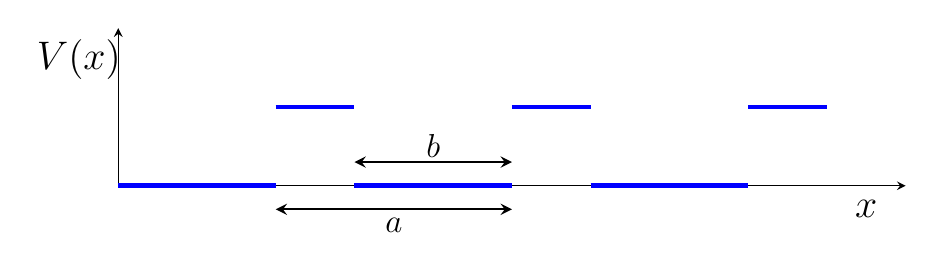
\begin{tikzpicture}
\draw[->] (0,0) -- (10,0);
\draw[->] (0,0) -- (0,2);
\draw[ultra thick, blue] (0,0) -- (2,0);
\draw[ultra thick, blue] (2,1) -- (3,1);
\draw[ultra thick, blue] (3,0) -- (5,0);
\draw[ultra thick, blue] (5,1) -- (6,1);
\draw[ultra thick, blue] (6,0) -- (8,0);
\draw[ultra thick, blue] (8,1) -- (9,1);
\draw[thick, <->] (2,-0.3) -- (5,-0.3);
\draw[thick, <->] (3,0.3) -- (5,0.3);
\node at (3.5, -0.5) {\large{$a$}};
\node at (4, 0.5) {\large{$b$}};
\node at (-0.5, 1.6) {\Large{$V(x)$}};
\node at (9.5, -0.3) {\Large{$x$}};
\end{tikzpicture}
\end{center}
results in energy bands of the form

\begin{center}
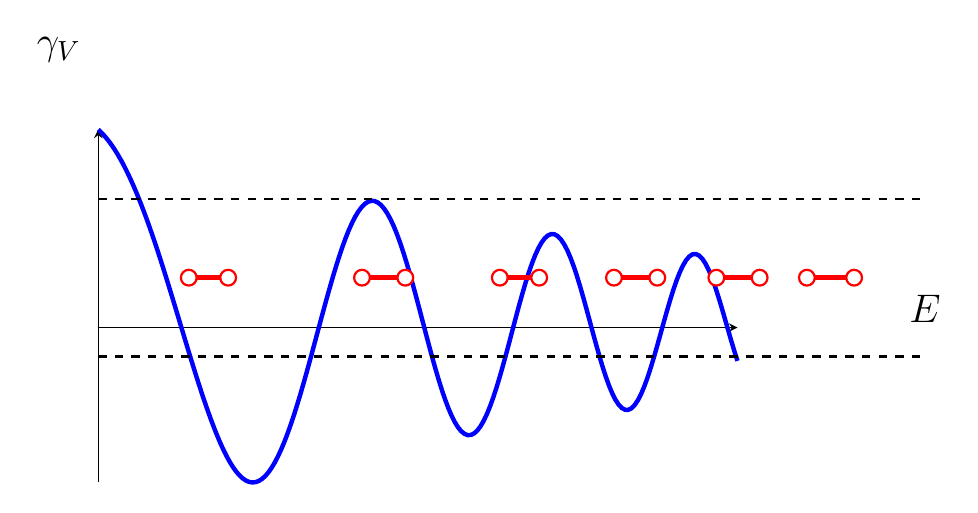
\begin{tikzpicture}
  \begin{axis}[
    trig format plots=rad,
    axis lines = middle,
    clip=false,
    ticks=none, 
    width=0.8\textwidth,
    height=0.5\textwidth
    ]
    \addplot[domain=0.42:1.5,samples=200,blue, ultra thick] {4*exp(-x)*sin(10*x^2)};
  \end{axis}
  \draw[thick, dashed] (0,3.6) -- (10.5,3.6); 
  \draw[thick, dashed] (0,1.6) -- (10.5,1.6);
  \draw[ultra thick, red] (1.15,2.6) -- (1.65,2.6);
  \draw[red, fill=white, thick] (1.15,2.6) circle [radius=0.1];
  \draw[red, fill=white, thick] (1.65,2.6) circle [radius=0.1];
  \draw[ultra thick, red] (3.35,2.6) -- (3.9,2.6);
  \draw[red, fill=white, thick] (3.35,2.6) circle [radius=0.1];
  \draw[red, fill=white, thick] (3.9,2.6) circle [radius=0.1];
  \draw[ultra thick, red] (5.1,2.6) -- (5.6,2.6);
  \draw[red, fill=white, thick] (5.1,2.6) circle [radius=0.1];
  \draw[red, fill=white, thick] (5.6,2.6) circle [radius=0.1];
  \draw[ultra thick, red] (6.55,2.6) -- (7.1,2.6);
  \draw[red, fill=white, thick] (6.55,2.6) circle [radius=0.1];
  \draw[red, fill=white, thick] (7.1,2.6) circle [radius=0.1];
  \draw[ultra thick, red] (7.85,2.6) -- (8.4,2.6);
  \draw[red, fill=white, thick] (7.85,2.6) circle [radius=0.1];
  \draw[red, fill=white, thick] (8.4,2.6) circle [radius=0.1];
  \draw[ultra thick, red] (9,2.6) -- (9.6,2.6);
  \draw[red, fill=white, thick] (9,2.6) circle [radius=0.1];
  \draw[red, fill=white, thick] (9.6,2.6) circle [radius=0.1];
  \node at (-0.5,5.5) {\Large{$\gamma_V$}};
  \node at (10.5,2.2) {\Large{$E$}};
\end{tikzpicture}
\end{center}
\newpage

\section{Relativistic Quantum Mechanics}
As we shall see the transition into relativistic quantum mechanics is highly non-trivial; in the sense that we don't simply add a new term onto our expressions that accounts for the relativistic effects. This lecture is meant as a very brief overview/introduction to quantum field theory, and so does not claim to be self contained in any sense. The main idea we want to highlight is how the ideas change once we start accounting for relativistic effects, and what the repercussions of those changes are. 

\subsection{Heuristic Derivation of the Schr\"{o}dinger Equation}

Schr\"{o}dinger recognised that he could obtain the Schr\"{o}dinger equation from the \emph{classical} energy-momentum relation
\bse 
E = \frac{p^2}{2m} + V,
\ese 
using the substitutions 
\bse 
E \squiggle i\hbar\partial_t, \qquad \qquad P_a \squiggle -i\hbar\partial_a
\ese 
giving 
\bse 
i\hbar\partial_t\psi = -\frac{\hbar^2}{2m}\partial_a\partial^a\psi + V\psi,
\ese 
for $\psi:\R^3\to\C$. 

If we want to get the probabilistic interpretation that quantum mechanics is built on, we need to introduce an object that
\ben[label=(\roman*)]
\item Is non-negative definite, 
\item Integrates to unity,
\item This integral doesn't change in time. 
\een 
As we have been using all along the such needed object is 
\bse 
\rho := |\psi|^2.
\ese 

We might ask ourselves `How does one come up with the idea to such an object?', the answer for which comes from the following. 

Firstly its clear that $\rho\geq 0$, by definition of the inner product. We can also always arrange for the integral over all space to be unity by normalisation. Now consider the Schr\"{o}dinger equation and its complex conjugate
\bi{rCl}
i\hbar\partial_t\psi & = & -\frac{\hbar^2}{2m}\partial_a\partial^a\psi + V\psi \\
-i\hbar\partial_t\overline{\psi} & = & -\frac{\hbar^2}{2m}\partial_a\partial^a\overline{\psi} + V\overline{\psi}.
\ei 
If we multiply the former from the right by $\overline{\psi}$ and the latter from the left by $\psi$, then subtract the two results we arrive, after rearranging a bit, at 
\bi{rCl}
\big[ (\partial_t\psi)\overline{\psi} + \psi(\partial_t\overline{\psi}) \big] & = & \frac{i\hbar}{2m} \big[ \psi(\partial_a\partial^a\overline{\psi}) - (\partial_a\partial^a\psi)\overline{\psi} \big] \\
\partial_t(\psi\overline{\psi}) & = & \frac{i\hbar}{2m}\partial_a \big[ \psi(\partial^a\overline{\psi}) - (\partial^a\psi)\overline{\psi}\big].
\ei
Then defining 
\bse 
\rho := \psi\overline{\psi}, \qquad \qquad j^a := -\frac{i\hbar}{2m} \big[ \psi(\partial^a\overline{\psi}) - (\partial^a\psi)\overline{\psi}\big],
\ese 
we arrive at the continuity equation
\bse 
\partial_t\rho + \partial_aj^a = 0,
\ese 
from which it follows that 
\bi{rCl}
\partial_t \int_{\R^3}d^3x \rho(x) & = & \int_{\R^3} d^3x (\partial_t\rho)(x) \\
& = & \int_{\R^3} d^3x (\partial_aj^a)(x) \\
& = & 0,
\ei
where we have used the fact that we are integrating over all of $\R^3$ (which has no boundary/surface) with the fact that $\partial_aj^a$ is a purely surface term. 

\subsection{Heuristic Derivation of the Relativistic Schr\"{o}dinger Equation (Klein-Gordan Equation)}

A note is made on the structural difference between non-relativistic spacetime and the spacetime of general relativity. For a much deeper discussion of this the reader is directed to Dr. Schuller's International Winter School on Gravity and Light\footnote{Available via \href{https://www.youtube.com/watch?v=7G4SqIboeig&t=3811s}{YouTube}.}

Schro\"{o}dinger, quite courageously, tried to apply the method of the previous section to the relativistic energy-momentum relation ($c=1$ here),
\bse
E^2 = p^2 + m^2,
\ese 
which gives 
\bse 
-\hbar^2\partial_t^2 = -\hbar^2\partial_a\partial^a + m^2,
\ese 
which, after rearranging, gives the so-called \emph{Klein-Gordan equation}\footnote{It is named such as Oskar Klein and Walter Gordan also arrived at this result after Schro\"{o}dinger, and proceeded to try and interpret it as the description of relativistic electrons, which we shall see shortly is not the case.}
\bse 
(\Box +m^2)\phi = 0,
\ese 
where we have introduced the d'Alembert operator 
\bse 
\Box := \partial_t^2 - \partial_a\partial^a.
\ese 

The question we now have to ask is `can we still obtain some probability interpretation using $\phi$?' The answer is no, as we shall now show. 

In correlation to the non-relativistic case, in order to ensure the integral is a constant in time, we wish to find a $J^{\mu}$ such that 
\bse 
\partial_{\mu}J^{\mu} = \partial_0J^0 + \partial_aJ^a = 0.
\ese 
Again similarly to before, by considering the Klein-Gordan equation and its complex conjugate we arrive at 
\bse 
J^{\mu} := (\partial^{\mu}\phi)\overline{\psi} - \psi (\partial^{\mu}\overline{\psi}),
\ese 
and Gauss' theorem tells us that the \emph{only} candidate for the probability amplitude $\rho$ is 
\bse 
\rho := J^0 := (\partial^0\phi)\overline{\psi} - \psi (\partial^0\overline{\psi}).
\ese 
This all looks fine, in fact it looks exactly like the non-relativistic case. However there is one subtle, yet highly important, difference. In the Schr\"{o}dinger equation we had only first order time derivatives, whereas the Klein-Gordan equation is second order in time derivatives. This means that for the latter we can prescribe as initial conditions not only $\phi(t)$ but its derivative $(\partial_t\phi)(t)$ at some time. We can thus choose these initial conditions such that $\rho<0$ at some time, which violates the interpretation of $\rho$ as a probability density. This is a problem that cannot be removed at this level, the reason for which we shall soon see.

\br 
Historically, Schr\"{o}dinger actually arrived at the relativistic equation first (as he knew this was ultimately where he wanted to go), however when running into the problem highlighted above he decided instead to consider the non-relativistic case and ended up with the Schr\"{o}dinger equation.
\er 

\br 
Note some people often refer to the time and spatial derivatives being on an \emph{equal footing} in the Klein-Gordan equation. This is a highly misleading choice of words. They are not on an equal footing, as the temporal derivatives come with a positive sign, whereas the spatial ones come with a negative sign. This is not just some little difference to be brushed over. Indeed, without this minus sign stems from Maxwell's equations, and without it the Klein-Gordan equation would be physically useless; the gist being that if time and space were on an equal footing then we would not be able to predict the future, which is the main driving force of physics. What people should say is that they are on a \emph{similiar} footing. 
\er 

\subsection{Dirac Equation}

So, as we have seen, it is this second derivative that causes us the problems, so the natural question is `How do we avoid it?' The immediate answer is to try considering 
\bse 
E = \sqrt{p^2+m^2},
\ese 
and then using the substitutions as above. However this is no better as now the RHS is the square root of a differential operator, and so in the expansion about $m^2$ we will end up with a theory with infinite spatial derivative order. Not good at all! 

Dirac then asked the question `What if I use a different substitution prescription such that the whole of the RHS becomes a single order derivative?' Following this thought, after several calculations, he arrives at the so-called \emph{Dirac equation} 
\bse 
(i\gamma^\mu\partial_\mu - m\b1_4)\Psi = 0,
\ese 
where the $\gamma^{\mu}$ are $4\times4$ matrices satisfying the anticommutation relation
\bse 
\{\gamma^{\mu},\gamma^{\nu}\} := \gamma^{\mu}\gamma^{\nu} + \gamma^{\mu}\gamma^{\nu} = 2\eta^{\mu\nu},
\ese 
known as the \emph{Dirac algebra}, where $\eta^{\mu\nu}$ is the Minkowski metric given by\footnote{Using the (-,+,+,+) signature.} 
\bse 
\eta^{\mu\nu} = \text{diag}(-1,1,1,1).
\ese 
The vector $\Psi$ here is a 4 component object known as a spinor, where (after some work) we can think of two of the components being a particle and the other two being the associated antiparticle. 

So the Dirac equation introduces antimatter into the mix, however it turns out that it still doesn't fix the probability problem addressed by the Klein-Gordan equation!

\subsection{The Deep Route of the Problem}

It turns out the problem stems from perhaps the most well-known equation in the world... $E=mc^2$, which tells us that we need not conserve particle number. For example the interaction between two particles could result in any number of resulting particles (provided the energy is in sufficiently large) 

\begin{center}
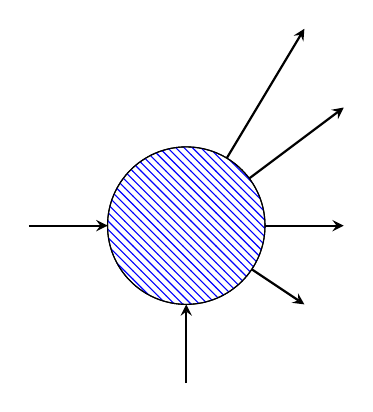
\begin{tikzpicture}
\draw[thick, ->] (1,0) -- (2,0);
\draw[thick, ->] (3,-2) -- (3,-1);
\draw[thick, ->] (3,0) -- (4.5,2.5);
\draw[thick, ->] (3,0) -- (5,1.5);
\draw[thick, ->] (3,0) -- (4.5,-1);
\draw[thick, ->] (3,0) -- (5,0);
\draw[fill=white] (3,0) circle [radius=1];
\draw[pattern=north west lines, pattern color=blue] (3,0) circle [radius=1];
\end{tikzpicture}
\end{center}

If this information is contained within $E=mc^2$, it is also contained in the relativistic energy-momentum equation $E^2= p^2 +m^2c^4$, and so we were unjustified to look for an equation in the relativistic context that describes \emph{one} (or any fixed number) of particles. In other words, our theory needs to account for this non-conservation of particle number, including have no particles (i.e. the vacuum). Mathematically the idea is to construct a direct sum of Hilbert spaces, each of which describes a different number of particles. This is known as the \emph{Fock space}, 
\bse 
\cF := \C \oplus \cH \oplus (\cH\otimes\cH) \oplus (\cH\otimes\cH\otimes\cH) \oplus ...
\ese 

We can then construct the inner product on $\cF$ from the inner products on the Hilbert spaces, all of which are obtained from the inner product on $\cH$. That is if $\psi,\varphi\in\cF$ given by 
\bi{rCl}
\psi & = & a_0 \oplus a_1 \psi_1 \oplus \sum_{ij} a_2^{ij} (\psi_{2i}\otimes\psi_{2j}) \oplus  ... \\
\varphi & = & b_0 \oplus b_1 \varphi_1 \oplus \sum_{ij} b_2^{ij} (\varphi_{2i} \otimes\varphi_{2j}) \oplus ...,
\ei
then the inner product is given by 
\bse 
\braket{\psi}{\varphi} = \overline{a_0}b_0 + \overline{a_1}b_1\braket{\psi_1}{\varphi_1}_{\cH} + \sum_{ijk\ell} \overline{a^{ij}_2}b^{k\ell}_2 \braket{\psi_{2i}\otimes\psi_{2j}}{\varphi_{2k}\otimes\varphi_{2\ell}}_{\cH\otimes\cH} + ...
\ese 

\br 
For the Klein-Gordan equation it is actually the \emph{symmetrised} tensor products we need, giving this symmetric Fock space
\bse 
\odot \cF := \C \oplus (\cH\odot\cH) \oplus (\cH\odot\cH\odot\cH) \oplus ...,
\ese 
and it describes \emph{bosonic} systems. 

Similarly for the Dirac equation we require the \emph{anti-symmetrised} tensor product, giving 
\bse 
\wedge \cF := \C \oplus (\cH\wedge\cH) \oplus (\cH\wedge\cH\wedge\cH) \oplus ...,
\ese 
which describes \emph{fermionic} systems.
\er 

We claim that once you lift the Klein-Gordan and Dirac equations onto their respective Fock spaces, that the problem of negative probability density vanishes. 

\subsection{Feynman Diagrams}

Richard Feynman developed a pictorial representation of the highly complicated interaction of particles. The basic idea is to take a perturbation expansion of the interaction and represent each order by a set of diagrams. The order of the diagram is associated with the number of so-called \emph{vertices} present. 

For example the first few terms for the process of electron-electron scattering would be drawn as:

% I had trouble with the Tikz-Feyman package in this file, so I drew this elsewhere and imported it as a picture.
\begin{center}
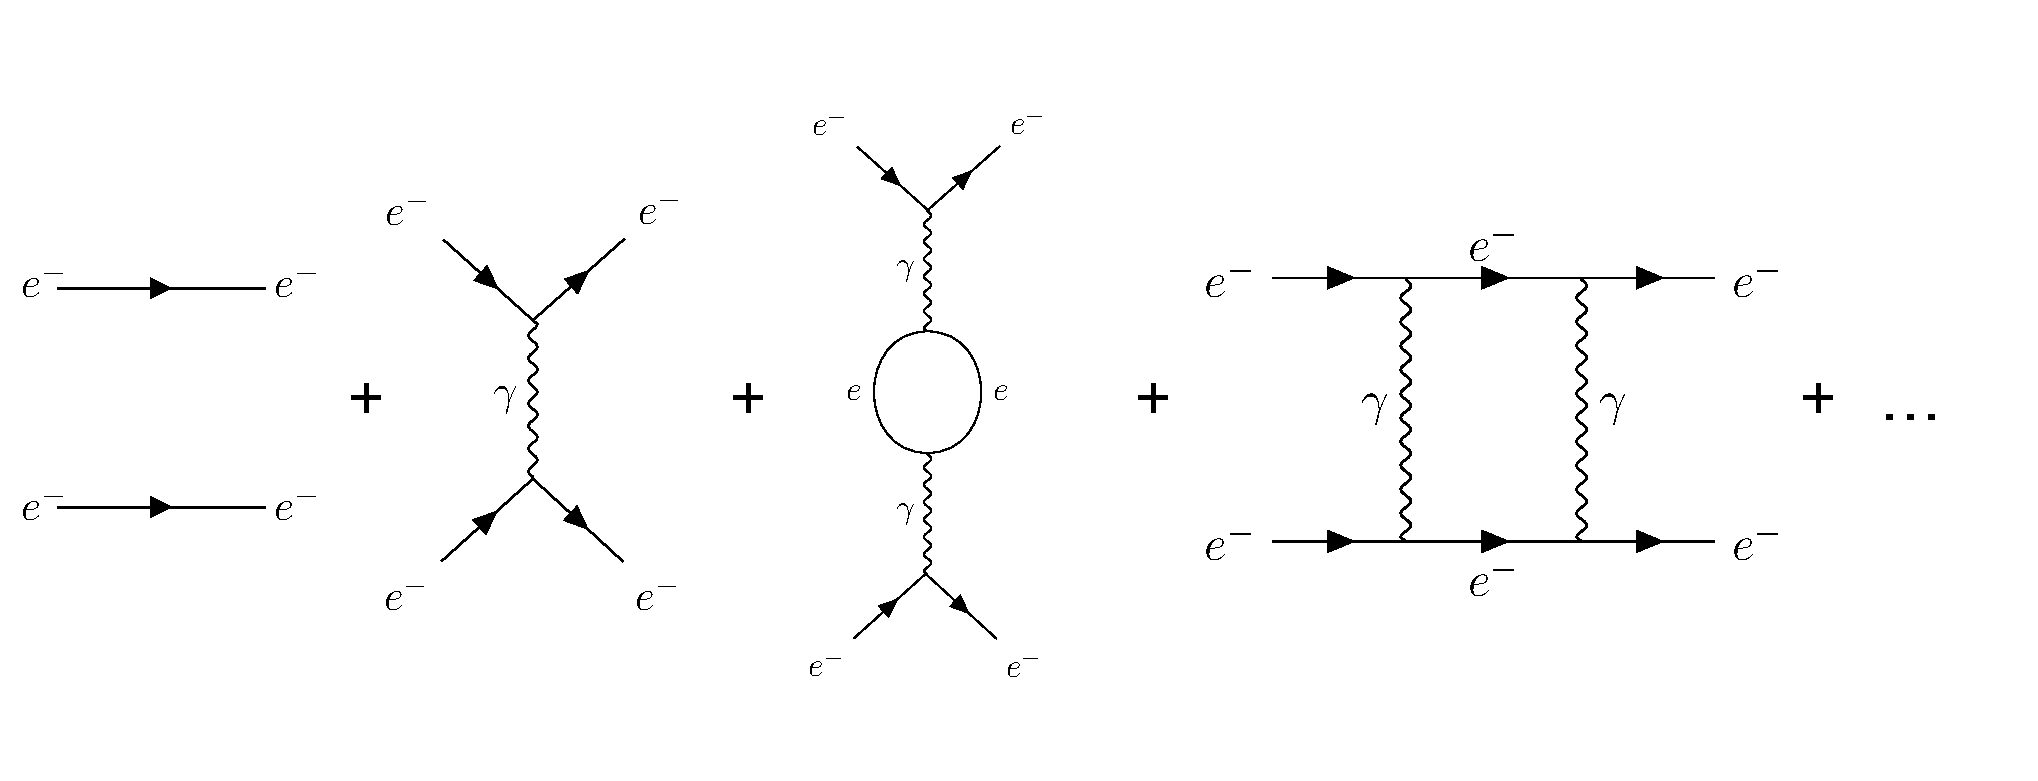
\includegraphics[scale=0.45, origin=c]{graphics/Feynman.pdf}
\end{center}

The first diagram (which has no vertices) is the zeroth order diagram, the second one (with two vertices) is the second order diagram and the last two (which both have 4 vertices) are the fourth order diagrams. The furthest most left and right arrows (i.e. the ones that have a non-vertexed end) are known as \emph{external lines}, and the other ones are known as \emph{internal lines}. Particles represented by internal lines are often referred to \emph{virtual} particles. 

\br 
One should be careful when it comes to drawing the arrows on the internal lines, however, as (unless the rest of the diagram indicates otherwise) we could have a particle or an antiparticle (whose arrow points the opposite way). It is for this reason that the so-called \emph{loop} in the third diagram does not have arrows. On the final diagram we do draw the arrows, as conservation of electric charge forces us to ensure our virtual particles are electrons (not positrons, the anti-electron). 

Note also on loop internal lines we have simply written $e$ and not $e^-$ or $e^+$ (the positron), this further indicates that we do not know which is which, only that one must be an electron and the other a positron. 
\er 

Mathematically Feynman diagrams correspond to integral equations, and there is a set of rules (cleverly named \emph{Feyman Rules}) which tell you how to convert the diagrams into these integrals. They are a indispensable tool when it comes to studying relativistic particle physics, as not only are they quicker to draw then writing out integrals, they have some incredibly elegant properties (such as so-called \emph{crossing symmetry}) which make the calculations significantly easier. However, we shall not go into any more detail here; the unfamiliar reader is directed to the massive resource of information in textbooks/on the internet. 
\newpage


\section*{Further readings}
\addcontentsline{toc}{section}{Further readings}

\subsection*{Mathematical quantum mechanics}

\begin{itemize}
\item Ballentine, \textit{Quantum Mechanics: A Modern Development} (Second edition), World Scientific 2014
\item Faddeev, Yakubovskii, \textit{Lectures on Quantum Mechanics for Mathematics Students}, American Mathematical Society 2009
\item Folland, \textit{Quantum Field Theory: A Tourist Guide for Mathematicians},  American Mathematical Society 2008
\item Gieres, \textit{Mathematical surprises and Dirac's formalism in quantum mechanics}\\
\url{https://arxiv.org/abs/quant-ph/9907069}
\item Hall, \textit{Quantum Theory for Mathematicians}, Springer 2013
\item Mackey, \textit{Mathematical Foundations of Quantum Mechanics}, Dover Publications 2004
\item Moretti, \textit{Spectral Theory and Quantum Mechanics: With an Introduction to the Algebraic Formulation}, Springer 2013
\item Parthasarathy, \textit{Mathematical Foundations of Quantum Mechanics}, Hindustan Book Agency 2005
\item Strocchi, \textit{An Introduction to the Mathematical Structure of Quantum Mechanics: A Short Course for Mathematicians}, World Scientific 2008
\item Takhtajan, \textit{Quantum Mechanics for Mathematicians}, American Mathematical Society 2008
\end{itemize}

\subsection*{Standard quantum mechanics textbooks}

\begin{itemize}
    \item Griffiths, \textit{Introduction to Quantum Mechanics} (Second edition), Cambridge University Press 2016
    \item Nazarov \& Danon, \textit{Advanced Quantum Mechanics}, Cambridge University Press, 2013
\end{itemize}


\subsection*{Linear Algebra}

\begin{itemize}
\item Friedberg, Insel, Spence, \textit{Linear Algebra} (4th Edition), Pearson 2002
\item J\"anich, \textit{Linear algebra}, Springer 1994
\item Lang, \textit{Linear Algebra} (Third edition), Springer 1987
\item Shakarchi, \textit{Solutions Manual for Lang's Linear Algebra}, Springer 1996
\end{itemize}


\subsection*{Topology}

\begin{itemize}
\item Adamson, \textit{A General Topology Workbook}, Birkh\"auser 1995
\item Kalajdzievski, \textit{An Illustrated Introduction to Topology and Homotopy}, CRC Press 2015
\item Munkres, \textit{Topology} (Second edition), Pearson 2014
\end{itemize}


\subsection*{Functional analysis}

\begin{itemize}
\item Aliprantis, Burkinshaw, \textit{Principles of Real Analysis (Third Edition)}, Academic Press 1998
\item Aliprantis, Burkinshaw, \textit{Problems in Real Analysis: A Workbook with Solutions}, Academic Press 1998
\item Day, \textit{Normed Linear Spaces}, Springer 1973
\item Halmos, \textit{A Hilbert Space Problem Book}, Springer 1982
\item Hunter, Nachtergaele, \textit{Applied Analysis}, World Scientific, 2001
\item Kadison, Ringrose, \textit{Fundamentals of the Theory of Operator Algebras. Volumes I-II}, American Mathematical Society 1997
\item Leoni, \textit{A first Course in Sobolev Spaces}, American Mathematical Society 2009
\item Rynne, Youngson, \textit{Linear Functional Analysis (Second Edition)}, Springer 2008
\item Serov, \textit{Fourier Series, Fourier Transform and Their Applcations to Mathematical Physics} Springer 2017
\end{itemize}


\subsection*{Measure theory and Integration}

\begin{itemize}
\item Bartle, \textit{A Modern Theory of Integration}, American Mathematical Society 2001
\item Bartle, \textit{Solutions Manual to A Modern Theory of Integration}, American Mathematical Society 2001
\item Halmos, \textit{Measure Theory}, Springer 1982
\item Nelson, \textit{A User-friendly Introduction to Lebesgue Measure and Integration}, American Mathematical Society 2015
\item Rana, \textit{An Introduction to Measure and Integration}, American Mathematical Society 2002
\end{itemize}






\newpage

%\printindex

\end{document}
